% !TEX encoding = UTF-8
\documentclass[12pt,a4paper]{report}
\usepackage[a4paper,margin=1in]{geometry}
\usepackage{iftex}
\ifPDFTeX
  \usepackage[T1]{fontenc}
  \usepackage[utf8]{inputenc}
  \usepackage{lmodern}
  \usepackage{textcomp}
\else
  \usepackage{fontspec}
  \setmainfont{Latin Modern Roman}
  \setsansfont{Latin Modern Sans}
  \setmonofont{Latin Modern Mono}
  \usepackage{unicode-math}
  \setmathfont{Latin Modern Math}
\fi
\usepackage{newunicodechar}
\newunicodechar{≥}{\ensuremath{\geq}}
\newunicodechar{≤}{\ensuremath{\leq}}
\newunicodechar{≈}{\ensuremath{\approx}}
\newunicodechar{λ}{\ensuremath{\lambda}}
\newunicodechar{κ}{\ensuremath{\kappa}}
\newunicodechar{Σ}{\ensuremath{\Sigma}}
\newunicodechar{√}{\ensuremath{\surd}}
\newunicodechar{×}{\ensuremath{\times}}
\newunicodechar{→}{\ensuremath{\rightarrow}}
\newunicodechar{∞}{\ensuremath{\infty}}
\newunicodechar{−}{\ensuremath{-}}
\usepackage{titlesec}
\titleformat{\chapter}[hang]{\Large\bfseries}{\thechapter.}{0.6em}{}
\titlespacing*{\chapter}{0pt}{0pt}{12pt}
\titleformat{name=\chapter,numberless}[hang]{\Large\bfseries}{}{0pt}{}
\titleformat{\section}{\large\bfseries}{\thesection}{0.6em}{}
\titleformat{\subsection}{\normalsize\bfseries}{\thesubsection}{0.6em}{}
\titleformat{\subsubsection}{\normalsize\itshape\bfseries}{\thesubsubsection}{0.6em}{}
\setlength{\headheight}{14.5pt}
\usepackage{microtype}
\usepackage{xcolor}
\usepackage{graphicx}
\usepackage{tikz}
\usepackage{float}
\usepackage{booktabs}
\usepackage{longtable}
\usepackage{array}
\usepackage{enumitem}
\usepackage{caption}
\usepackage{fancyhdr}
\usepackage{listings}
\usepackage{tcolorbox}
\tcbuselibrary{breakable}
\usepackage{pdfpages}
\usepackage[nottoc]{tocbibind}
\usepackage{rotating}
\usepackage{adjustbox}
\usepackage{makeidx}
\usepackage[toc]{glossaries}
\usepackage[hidelinks,pdftitle={Unified Adaptive Memory Manager for KV-Cache Management on Edge Processors},pdfauthor={Ishanvi Prasad, Sweety}]{hyperref}
\makeindex
\makeglossaries
\setlength{\parindent}{0pt}
\emergencystretch=3em
\setlength{\parskip}{5pt}
\linespread{1.0}
\setcounter{secnumdepth}{4}
\setcounter{tocdepth}{1}
\setlist{itemsep=2pt,topsep=3pt,parsep=0pt}
\captionsetup{font=small,labelfont=bf,skip=4pt}
\captionsetup[longtable]{font=small,labelfont=bf,skip=4pt}
\renewcommand{\topfraction}{0.9}\renewcommand{\bottomfraction}{0.9}\renewcommand{\textfraction}{0.08}\renewcommand{\floatpagefraction}{0.8}
\pagestyle{fancy}\fancyhf{}
\fancyhead[L]{\small ELL305 Termpaper}
\fancyhead[R]{\small Ishanvi Prasad (2024EE10406), Sweety (2024MT10535)}
\fancyfoot[C]{\small\thepage}
\renewcommand{\headrulewidth}{0.3pt}
\fancypagestyle{plain}{\fancyhf{}\fancyfoot[C]{\small\thepage}\renewcommand{\headrulewidth}{0pt}}
\lstset{basicstyle=\ttfamily\fontsize{7.5}{9}\selectfont,breaklines=true,breakatwhitespace=false,columns=fullflexible,keepspaces=true,
  frame=single,framerule=0.3pt,backgroundcolor=\color{black!4},xleftmargin=2pt,xrightmargin=2pt,aboveskip=4pt,belowskip=4pt,showstringspaces=false,
  postbreak=\mbox{\space\space}}
\newtcolorbox{calloutbox}[1]{breakable,colback=black!5,colframe=black,boxrule=0.4pt,arc=0pt,title={#1},fonttitle=\bfseries,
  coltitle=black,colbacktitle=black!12,left=5pt,right=5pt,top=3pt,bottom=3pt,before skip=6pt,after skip=8pt}
\usetikzlibrary{arrows.meta}
\newglossaryentry{kvcache}{name={KV cache},description={Stored keys and values of all previous tokens, per layer and head.}}
\newglossaryentry{block}{name={Block},description={Fixed group of 16 consecutive tokens; the unit of placement.}}
\newglossaryentry{tier}{name={Tier},description={A memory level: T0 SRAM, T1 and T2 DRAM, T3 flash.}}
\newglossaryentry{codec}{name={Codec},description={Storage format of a block: FP16, INT8, 4-bit or 2-bit, optionally entropy-coded. Our own term.}}
\newglossaryentry{heavy}{name={Heavy hitter},description={A token that collects a large share of attention.}}
\newglossaryentry{sink}{name={Attention sink},description={The first tokens, which attract attention whatever their content.}}
\newglossaryentry{ratchet}{name={Precision ratchet},description={Rule that a block's precision may only go down.}}
\newglossaryentry{hyst}{name={Hysteresis},description={Rule that blocks a move unless it is clearly better than staying.}}
\newglossaryentry{recall}{name={Attention-mass recall},description={Share of the dense attention probability that falls on the tokens that were read.}}
\newglossaryentry{rvv}{name={RVV},description={RISC-V Vector extension.}}
\newglossaryentry{vcd}{name={VCD},description={Value change dump: the waveform file a simulator writes, opened in GTKWave.}}
\newglossaryentry{hh}{name={H2O},description={Heavy-Hitter Oracle: keeps tokens with the largest accumulated attention.}}
\newglossaryentry{kivi}{name={KIVI},description={Quantisation scheme that scales keys per channel and values per token.}}
\newglossaryentry{quest}{name={Quest},description={Query-aware selection of KV blocks using per-block min/max key bounds.}}
\newglossaryentry{ara}{name={Ara},description={Open-source RISC-V vector processor.}}
\newglossaryentry{rtl}{name={RTL},description={Register-transfer level hardware description, here written in Verilog.}}
\newglossaryentry{uamm}{name={UAMM},description={Unified Adaptive Memory Manager, the name of our design (UAMM-1 and UAMM-2).}}
\newglossaryentry{planner}{name={Planner},description={The routine that picks a (tier, codec) pair for each block by comparing costs.}}
\newglossaryentry{lambda}{name={Quality weight},description={The factor lambda that scales the quantisation-error term in the planner cost.}}
\begin{document}
\begin{titlepage}\centering\vspace*{2.2cm}
{\fontsize{34}{40}\selectfont\bfseries Termpaper\par}\vspace{0.5cm}{\fontsize{26}{30}\selectfont\bfseries ELL305\par}\vspace{1.4cm}
{\fontsize{22}{26}\selectfont\bfseries Unified Adaptive Memory Manager\par}\vspace{0.3cm}{\large for Key--Value Cache Management in Large Language Model Inference on Edge Processors\par}\vspace{1.4cm}
{\Large\bfseries Ishanvi Prasad (2024EE10406)\par}\vspace{0.2cm}{\Large\bfseries Sweety (2024MT10535)\par}\vspace{1.4cm}
{\bfseries Source code:} \url{https://github.com/IshanviPrasad29/uamm2-kv-cache-manager}\par\vfill{\small Department of Electrical Engineering, IIT Delhi}\end{titlepage}
\chapter*{Copyright Assignment}
All intellectual property rights (IPR) arising from this work belong to the Indian Institute of Technology Delhi (IIT Delhi). In the case of cited material, the intellectual property rights belong to the respective authors of the original sources.

\vspace{1.2cm}
Ishanvi Prasad\\
2024EE10406\\
\medskip\\
Sweety\\
2024MT10535\\
\clearpage
\chapter*{Acknowledgements}
We thank the course instructor for the guidance he gave us while this term paper took shape. The discussions at the start, when we were still deciding what the problem was, saved us a lot of time.

We also thank the Department of Electrical Engineering, IIT Delhi, for the academic environment and the computing facilities, and the Institute library for access to the papers we needed.

The open source tools we used (Verilator, Yosys, GTKWave, NumPy, matplotlib and others) made it possible for us to build and check our hardware design on ordinary machines. We are grateful to the people who maintain them.

\vspace{1.2cm}
Ishanvi Prasad\\
Sweety\\
\clearpage
\chapter*{Abstract}\addcontentsline{toc}{chapter}{Abstract}
A language model that runs on a small processor has plenty of arithmetic available. What it lacks is memory. Every generated token adds a key and a value vector to the KV cache for each layer and head, the cache has to be read again at the next token, and it shares a few gigabytes with the model weights. When the cache outgrows the fast memory, the processor spends its time moving data.

This paper describes how we approached that problem. We first built UAMM-1, a memory manager that splits the cache into blocks, scores each block with an H2O-style importance value and places it in one of three memory tiers using fixed thresholds. Reviewing it, we found that it had no way of making data smaller, so when memory ran out it could only delete tokens, hence accuracy was less. We then built UAMM-2, in which a block is stored in a (tier, codec) pair. Cold blocks are compressed to 8, 4 or 2 bits instead of being deleted, a utility planner chooses the pair for each block, precision can only go down, and attention reads only the blocks that can matter for the current query. We also wrote three Verilog blocks and a RISC-V vector kernel for the inner loops.

On a synthetic trace with assumed memory costs, a 168 KB budget holds 1,536 tokens that FP16 would need 393 KB for. UAMM-1 had to delete 63 \% of the tokens to fit; UAMM-2 keeps all of them with a mean attention-output error between 0.12 and 0.17 ( all these came as results of simulations). A simple baseline that stores every block in 4-bit also fits and is faster in our model, so our planner adds lower error at the same size, a smaller size, and the ability to cope with tighter budgets. The Verilog blocks match their software models bit for bit and every injected fault was caught. The vector kernel was compiled but never run, no real language model was used, and the latency figures are assumptions. The report states these limits where each result appears, lists the future scopes, and gives the repository in which all of the work can be reproduced.

\clearpage
\tableofcontents\clearpage
\pagenumbering{arabic}
\chapter{Problem Description}
Large language models (LLMs) have moved from data centre curiosities to components that product teams now want inside phones, laptops, vehicles, wearables, industrial controllers and embedded boards. The motivations are practical and well understood: \textbf{latency} (no network round trip), \textbf{privacy} (prompts and documents never leave the device), \textbf{availability} (the feature works offline) and \textbf{cost} (no per-token cloud bill). This report is about one specific obstacle that stands between the idea and a working product: the memory that a running LLM needs for its \textit{attention history}, the \textbf{key value (KV) cache}, and how that memory can be managed on the small, power constrained processors that live at the edge.

The report is organised as follows. Chapter~1 (this chapter) describes the problem. Chapter~2 is the literature review: the textbook chapters and the research papers we read, what we learned from each and how we used it. Chapter~3 is a step-wise mind map of the whole project. Chapter~4 covers UAMM-1\index{UAMM-1}: how we reached the problem, what the prototype is, the gaps we found in it, and its code, how to run it and where its data comes from. Chapter~5 covers UAMM-2\index{UAMM-2}: the design, the code, the decisions we made by experiment or by reasoning, and the problems we found and corrected. Chapter~6 gives the simulation and hardware (verilog) results, what we assumed and what we think is new. Chapter~7 lists the future scope. Chapter~8 is the project timeline and Chapter~9 explains how to set up the repository with Git and summarises the work. The references come next. The appendices hold the readability indices, raw tables and source listings. The lists of tables and figures, the glossary and the index are at the end.

\section{Why LLMs on edge devices at all}\label{sec:1_1}
An \textit{edge processor} in this report means a processor that runs the model locally rather than in a data centre: a mobile application processor, an embedded RISC-V\index{RISC-V} or Arm SoC, a single-board computer, a small NPU-equipped module. Typical constraints, compared with a data-centre accelerator, are shown in the table below.

{\fontsize{8}{9.5}\selectfont\setlength{\tabcolsep}{3pt}
\begin{longtable}{>{\raggedright\arraybackslash}p{0.99in}>{\raggedright\arraybackslash}p{1.35in}>{\raggedright\arraybackslash}p{1.81in}>{\raggedright\arraybackslash}p{1.72in}}
\caption{Order-of-magnitude comparison between a data-centre accelerator and an edge SoC. Ranges are representative, not measurements of one device.}\\
\toprule
\textbf{Resource} & \textbf{Data-centre accelerator} & \textbf{Edge SoC (typical range)} & \textbf{Consequence} \\\midrule\endfirsthead
\toprule \textbf{Resource} & \textbf{Data-centre accelerator} & \textbf{Edge SoC (typical range)} & \textbf{Consequence} \\\midrule\endhead
\bottomrule\endfoot
Memory capacity & 80–192 GB HBM per accelerator & 2–16 GB shared LPDDR, often shared with the OS and other apps & Weights and KV cache compete for the same few gigabytes \\
Memory bandwidth & 2–5 TB/s (HBM) & 10–60 GB/s (LPDDR4/5) & Two orders of magnitude less; decode is bandwidth-bound \\
Compute & Hundreds of TFLOP/s & 0.1–40 TOPS (NPU/GPU/vector unit) & Compute is rarely the first limit during decoding \\
Power / thermal & 300–700 W & 2–15 W sustained & Every DRAM access costs energy that the battery must pay \\
Storage tier & NVMe, network storage & eMMC / UFS / SD flash & Flash exists but is 10–100× slower than DRAM \\
Batching & Dozens of concurrent requests & Usually one user, one sequence & Batching cannot amortise weight reads \\
\bottomrule
\end{longtable}}
The right-hand column is the crux. Almost every technique that makes LLM serving efficient in the cloud relies on batching many requests together so that each read of the weights is shared by many sequences. An edge device typically serves one sequence at a time, so the cost of reading the model is paid by a single user. That makes the work of decoding a single token almost entirely a question of how many bytes must be moved from memory, which is why memory, not arithmetic, is the central resource on the edge.

\section{How an LLM generates text: prefill and decode}\label{sec:1_2}
A decoder-only transformer produces text one token at a time. Generation has two phases with very different hardware behaviour.

\begin{itemize}
\item \textbf{Prefill.} The prompt (say 1,000 tokens) is processed in parallel. All prompt tokens are pushed through every layer at once. The work is dominated by matrix–matrix multiplications and is compute-bound; hardware with strong vector or matrix units handles it well.
\item \textbf{Decode.} Each new token is produced by one pass through the network. For that single token the processor must read essentially every weight of the model, and in every attention layer it must also read the stored keys and values of every previous token. The work is matrix–vector multiplication, which performs very little arithmetic per byte moved, and is therefore memory-bandwidth-bound.
\end{itemize}
Because users experience decode as the streaming speed of the answer (tokens per second), and because the decode loop repeats for every token, the number of bytes read per token is the primary determinant of perceived speed on an edge device.

\section{What the KV cache is}\label{sec:1_3}
Inside every attention layer, each token produces three vectors from its hidden state: a \textbf{query} (q), a \textbf{key} (k) and a \textbf{value} (v). Attention for the newest token computes a similarity score between its query and the key of every earlier token, converts the scores into weights with a softmax, and returns the weighted sum of the earlier tokens' values:

\begin{center}\small\textit{o\_\allowbreak{}t = Σ\_\allowbreak{}\{i ≤ t\} softmax\_\allowbreak{}i( q\_\allowbreak{}t · k\_\allowbreak{}i / √d ) · v\_\allowbreak{}i}\end{center}
The keys and values of earlier tokens never change once computed (the model is causal). Recomputing them for every new token would multiply the work enormously, so inference engines store them. This store is the \textbf{KV cache\index{KV cache}}. It is the model's working memory of the conversation: every layer, every KV head, every token contributes one key vector and one value vector that must be kept for as long as the token can still be attended to.

The size of that memory follows a simple formula:

\begin{center}\small\textit{bytes per token = 2 (K and V) × layers × KV-heads × head-dim × bytes per element}\end{center}
and the cache for one sequence is that number multiplied by the current context length. Unlike the weights, which are a fixed size, the KV cache\index{KV cache} \textbf{grows with every generated token} and, in a multi-turn session or a document-question task, may become the largest single object in memory.

{\fontsize{8}{9.5}\selectfont\setlength{\tabcolsep}{3pt}
\begin{longtable}{>{\raggedright\arraybackslash}p{1.14in}>{\raggedright\arraybackslash}p{1.14in}>{\raggedright\arraybackslash}p{1.05in}>{\raggedright\arraybackslash}p{0.79in}>{\raggedright\arraybackslash}p{0.79in}>{\raggedright\arraybackslash}p{0.79in}}
\caption{KV-cache size for four illustrative model geometries (FP16, one sequence). Geometries are representative of model families, not of any specific checkpoint.}\\
\toprule
\textbf{Illustrative geometry} & \textbf{layers / KV heads / head-dim} & \textbf{bytes per token (FP16)} & \textbf{4K context} & \textbf{32K context} & \textbf{128K context} \\\midrule\endfirsthead
\toprule \textbf{Illustrative geometry} & \textbf{layers / KV heads / head-dim} & \textbf{bytes per token (FP16)} & \textbf{4K context} & \textbf{32K context} & \textbf{128K context} \\\midrule\endhead
\bottomrule\endfoot
TinyLlama-like & 22 / 4 / 64 & 22,528 & 88 MiB & 0.69 GiB & 2.8 GiB \\
Llama-3-8B-like & 32 / 8 / 128 & 131,072 & 512 MiB & 4.00 GiB & 16.0 GiB \\
7B MHA-style & 32 / 32 / 128 & 524,288 & 2,048 MiB & 16.00 GiB & 64.0 GiB \\
Llama-3-70B-like & 80 / 8 / 128 & 327,680 & 1,280 MiB & 10.00 GiB & 40.0 GiB \\
\bottomrule
\end{longtable}}
\begin{figure}[htbp]
\centering
\adjustbox{max width=\linewidth}{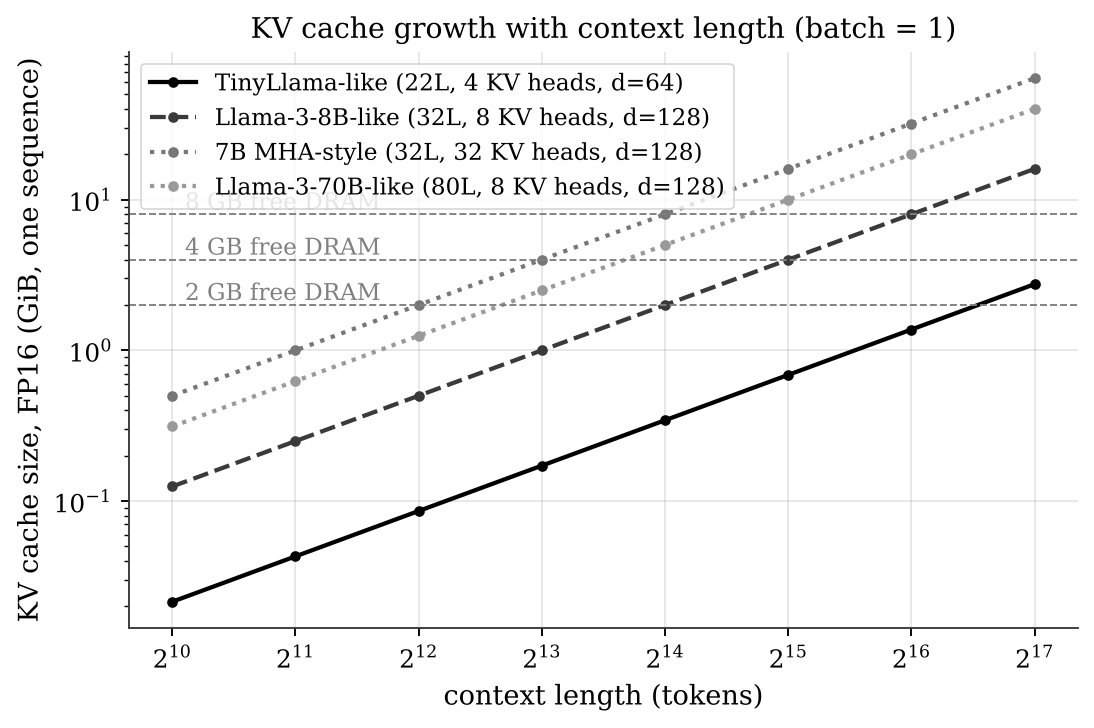
\includegraphics[width=6.10in,height=6.30in,keepaspectratio]{figs/f01_kv_growth.png}}
\caption{KV-cache size grows linearly with context. Dashed lines show plausible free-DRAM budgets on edge devices; every geometry except the smallest crosses one of them within the context lengths that applications now request.}
\end{figure}
\section{Why the KV cache is the bottleneck on the edge}\label{sec:1_4}
\subsection{Capacity}\label{sec:1_4_1}
On a phone with 8 GB of RAM, the operating system and foreground applications may leave 3–5 GB available to an on-device model. A 7–8-billion-parameter model quantised to 4 bits needs roughly 4–5 GB for its weights alone. The weights are fixed, so what remains for the KV cache\index{KV cache} shrinks to a few hundred megabytes. In the Llama-3-8B-like geometry of Table 2 that budget\index{budget} is exhausted at about 2–3 thousand tokens of FP16\index{FP16} cache, far short of the 32K–128K contexts that long-document and agentic applications need. When memory is exhausted the platform kills the process, or the engine must truncate the context, or the application must refuse the request.

\subsection{Bandwidth}\label{sec:1_4_2}
Capacity is only half of the problem. Standard attention reads \textbf{the entire KV cache\index{KV cache} for every generated token}. Even if the cache fits, its size determines how many bytes are moved per token, and therefore the maximum speed. The next figure shows the upper bound on decode speed imposed by KV reads alone for a 12.8 GB/s memory system, ignoring weight reads and compute. For a 7B-class model with full multi-head attention the bound drops below ten tokens per second at roughly 3K tokens of context, before a single weight has been read.

\begin{figure}[htbp]
\centering
\adjustbox{max width=\linewidth}{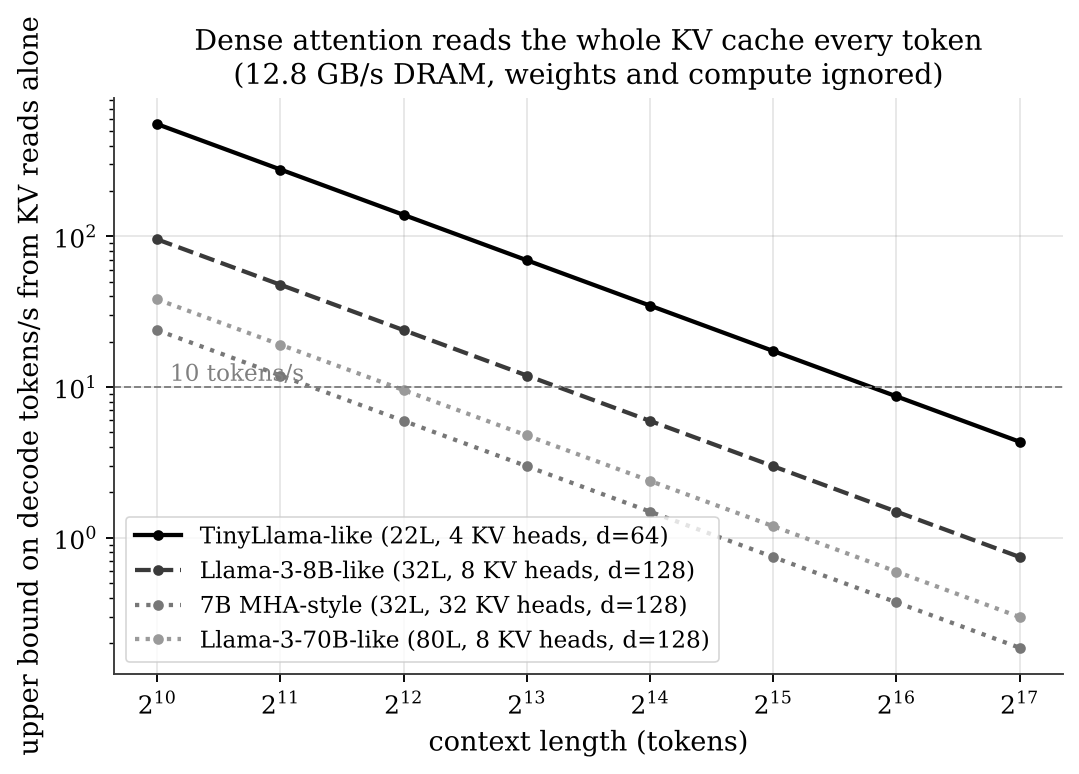
\includegraphics[width=6.10in,height=6.30in,keepaspectratio]{figs/f02_kv_bandwidth_bound.png}}
\caption{Upper bound on decode speed from KV-cache reads alone (12.8 GB/s DRAM). The curves fall as 1/context: this is the bandwidth wall that appears even when the cache fits in memory.}
\end{figure}
\subsection{Energy}\label{sec:1_4_3}
Each byte read from DRAM costs on the order of tens to a hundred times more energy than an arithmetic operation on that byte, and flash\index{flash} costs more again. A design that reads the whole cache for every token spends the battery on data movement. Reducing the bytes touched per token is therefore both a speed and a battery-life objective.

\subsection{Heterogeneous memory}\label{sec:1_4_4}
Edge SoCs expose a \textit{hierarchy}: a few tens of kilobytes of tightly coupled SRAM or vector register file next to the compute unit, gigabytes of DRAM behind a shared bus, and gigabytes of flash\index{flash} behind a controller. The hierarchy is an opportunity (cold data can be parked cheaply) and a hazard (a wrong placement decision puts hot data behind a slow link). Data-centre inference engines were not designed around this hierarchy, and most KV-cache research assumes a GPU with high-bandwidth memory and a host CPU as the only second tier\index{tier}.

\subsection{Why “just buy more memory” is not an answer}\label{sec:1_4_5}
For consumer and embedded products the memory is part of the bill of materials, shares a thermal envelope with the processor and is soldered. The memory in a shipped device cannot be upgraded after the fact, whereas the context lengths that applications demand grow every year. Any solution must therefore make the same hardware serve longer contexts and do so within a fixed energy budget\index{budget}.

\section{Why the obvious fixes fall short}\label{sec:1_5}
{\fontsize{8}{9.5}\selectfont\setlength{\tabcolsep}{3pt}
\begin{longtable}{>{\raggedright\arraybackslash}p{1.54in}>{\raggedright\arraybackslash}p{1.45in}>{\raggedright\arraybackslash}p{2.98in}}
\caption{Single-technique fixes and why each leaves part of the problem open.}\\
\toprule
\textbf{Obvious fix} & \textbf{What it gets you} & \textbf{Why it is not sufficient alone} \\\midrule\endfirsthead
\toprule \textbf{Obvious fix} & \textbf{What it gets you} & \textbf{Why it is not sufficient alone} \\\midrule\endhead
\bottomrule\endfoot
Truncate the context to a fixed window & Bounded memory and bandwidth & Discards information the model may need; quality collapses on tasks that refer back to early content \\
Store the cache in FP16 but page it to flash & Capacity & A flash read per token is far too slow; without knowing which blocks matter the system stalls \\
Quantise the entire cache uniformly to 4 bits & ≈3× capacity and bandwidth & Applies the same precision to important and unimportant data; still reads everything each token; 2-bit quantisation hurts quality \\
Evict low-importance tokens permanently & Capacity and bandwidth & Irreversible: a token that becomes relevant later is gone; no precision control for what remains \\
Use a bigger or smaller model & Moves the problem & Smaller models lose quality; the KV cache of any model still grows with context \\
\bottomrule
\end{longtable}}
Each fix addresses one dimension (capacity, bandwidth, precision, placement) and ignores the others. The central observation behind this work is that these dimensions interact: the best precision for a block depends on where it is stored, how likely it is to be read, and how much room is left. A system that decides them separately will make poor joint decisions.

\section{Problem statement and design requirements}\label{sec:1_6}
We therefore pose the problem as follows.

\begin{calloutbox}{Problem statement}
Given an autoregressive LLM decoding one sequence on an edge processor with a small fast memory, a larger DRAM and a slow flash\index{flash} tier\index{tier}, keep the KV cache\index{KV cache} within a fixed byte budget\index{budget} and reduce the bytes read per token, while keeping the attention output as close as possible to what an unconstrained FP16\index{FP16} dense implementation would produce, without irreversibly discarding information unless explicitly allowed.

\end{calloutbox}
One word needs explaining before the list. We use \textbf{codec\index{codec}} for the way a block of keys and values is stored in memory: as plain FP16\index{FP16}, or squeezed to 8, 4 or 2 bits, optionally with a lossless zlib layer on top. It is our own word for this storage format, not a standard term. From the problem statement we derived the requirements that shaped the design:

\begin{enumerate}
\item \textbf{Unit of management is a block, not a token.} Per-token bookkeeping is too costly and defeats memory locality; paging into fixed-size blocks makes allocation, migration\index{migration} and hardware tables simple.
\item \textbf{Placement and precision are decided together.} A block is placed in a (tier\index{tier}, codec\index{codec}) pair; the two choices are never made independently.
\item \textbf{Importance must be measured, not assumed.} Block priority must come from what attention actually does, not only from age.
\item \textbf{Reads must be selective.} The system should be able to skip fetching and decoding blocks that provably cannot matter for the current query.
\item \textbf{Loss must be controlled and visible.} Precision may only decrease along an explicit ratchet; permanent drop is opt-in; capacity overflow is reported rather than hidden.
\item \textbf{Decisions must be cheap enough for hardware.} The inner scoring loop must be implementable without a divider and verified bit-exactly against a software model.
\item \textbf{The design must connect to real runtimes and real vector hardware.} The codecs must be swappable, the compute kernel must target a RISC-V\index{RISC-V} vector unit, and a runtime adapter must isolate the engine from a specific inference framework.
\end{enumerate}
The rest of the report shows how each requirement was met, how it was tested, and where it is still unmet.

\chapter{Literature Review}\label{sec:2}
Before we designed anything we read through existing research done about the KV cache\index{KV cache}. This chapter goes through that reading. We first list the parts of the computer-architecture textbook by Sarangi [27] that we used, and then take the research papers one family at a time. For every paper we write what it does, what it solves, what it leaves open for a small edge device, and what we learned from it and used. The reference numbers in square brackets point to the list at the end of the report.

\begin{calloutbox}{Words used in this report}
\textbf{UAMM-1\index{UAMM-1}} and \textbf{UAMM-2\index{UAMM-2}} are the two systems we built. They are described in the next chapter, so the boxes below only say how each paper shaped them.

\textbf{Codec} is our own word, not a standard one. It means the storage format of a block of keys and values: FP16\index{FP16} (no compression), INT8\index{INT8}, 4-bit or 2-bit, optionally with a lossless zlib layer on top. UAMM-2\index{UAMM-2} chooses one for every block. When we describe a paper below we usually say "quantisation\index{quantisation} scheme" for the same idea.

\textbf{Tier} is a level of memory: the small fast memory next to the processor, DRAM, and flash\index{flash}.

\end{calloutbox}
\section{What we took from the architecture textbook}\label{sec:2_0}
Smruti R. Sarangi's \textit{Basic Computer Architecture} [27] is the book for our course. We went back to it at several points, mostly to check that what we were designing made sense as hardware. The table lists the chapters we used and what for. It is a map of where each idea came from, not a summary of the book.

{\fontsize{9}{10.5}\selectfont\setlength{\tabcolsep}{3pt}
\begin{longtable}{>{\raggedright\arraybackslash}p{1.70in}>{\raggedright\arraybackslash}p{4.36in}}
\caption{Chapters of Sarangi's Basic Computer Architecture [27] and how we used them.}\\
\toprule
\textbf{Chapter of the book} & \textbf{What we used it for in this work} \\\midrule\endfirsthead
\toprule \textbf{Chapter of the book} & \textbf{What we used it for in this work} \\\midrule\endhead
\bottomrule\endfoot
The Language of Bits & Number formats: why FP16, INT8 and 4-bit values behave differently, and how a fixed-point number such as our Q4.12 reciprocal is stored. \\
RISC-V Assembly Language & Background for the RISC-V vector extension that our kernel targets, and for reading the vector instructions the compiler produced. \\
Logic Gates, Registers, and Memories & Registers, SRAM and flip-flops, which we needed to build the block table and to understand why it appears as flip-flops in synthesis. \\
Computer Arithmetic & Multiplication and division in hardware. This is why the scorer uses weights that sum to 256 and shifts instead of dividing by 100, and why the quantiser multiplies by a stored reciprocal. \\
Processor Design & How a small controller and datapath are organised, which guided how we wrote the sweep scorer as a simple state machine. \\
Principles of Pipelining & Splitting the codec into stages so that it can handle 16 values per beat. \\
The Memory System & The memory hierarchy, locality, caches and page tables. A block table that maps a logical block to a tier and a slot is the same idea as a page table, and our tiers follow the same cost-versus-size logic. \\
I/O and Storage Devices & Flash storage: large units, slow access and limited writes, which shaped the rule that only cold, compressed blocks go to the flash tier. \\
\bottomrule
\end{longtable}}
\section{A taxonomy of approaches}\label{sec:2_1}
KV-cache research can be organised by \textit{which lever it pulls}. The table below lists the levers; the rest of the chapter takes them in turn.

{\fontsize{8}{9.5}\selectfont\setlength{\tabcolsep}{3pt}
\begin{longtable}{>{\raggedright\arraybackslash}p{1.07in}>{\raggedright\arraybackslash}p{1.78in}>{\raggedright\arraybackslash}p{2.05in}>{\raggedright\arraybackslash}p{0.98in}}
\caption{Levers used by the existing work.}\\
\toprule
\textbf{Lever} & \textbf{Idea} & \textbf{Representative work} & \textbf{Primary saving} \\\midrule\endfirsthead
\toprule \textbf{Lever} & \textbf{Idea} & \textbf{Representative work} & \textbf{Primary saving} \\\midrule\endhead
\bottomrule\endfoot
Change the model & Fewer KV heads, or a compressed latent KV & MQA, GQA, multi-head latent attention (DeepSeek-V2) & Bytes per token (requires training) \\
Manage memory better & Page the cache into blocks to remove fragmentation & PagedAttention / vLLM & Wasted capacity \\
Evict tokens & Keep only tokens judged important & H2O, Scissorhands, StreamingLLM, SnapKV, FastGen, PyramidKV & Capacity and bandwidth (lossy, irreversible) \\
Select at read time & Keep everything but fetch only relevant blocks & Quest, InfiniGen & Bandwidth \\
Quantise & Store K and V in fewer bits & KIVI, KVQuant & Capacity and bandwidth \\
Low-rank / projection & Store low-rank projections of K/V & Palu & Capacity and bandwidth \\
Offload & Spill to CPU memory or flash and prefetch & FlexGen, InfiniGen, LLM in a flash & Capacity \\
Joint systems & Combine compression, eviction and tiering & EvicPress, KV-Compress, TensorRT-LLM KV-compression framework & Several at once \\
Hardware engines & Dedicated logic for compress/decompress or cache control & hardware KV-compression engines, CXL-SpecKV, Ara vector unit & Energy and throughput \\
Deployment runtimes & Compile and run models portably on many devices & MLC LLM (TVM-based) & Portability \\
\bottomrule
\end{longtable}}
\section{Changing the attention architecture}\label{sec:2_2}
\subsection{Multi-query attention (MQA) [15] and grouped-query attention (GQA) [16]}
Shazeer's multi-query attention (2019) shares one key head and one value head across all query heads; Ainslie et al.'s grouped-query attention (2023) interpolates, sharing each KV head across a group of query heads. Both reduce the KV cache\index{KV cache} by the ratio of query heads to KV heads without changing the sequence length dimension. They are now standard in many open models (the 8-KV-head geometry used in Chapter 1 is an example).

\textbf{Limit.} They must be built into the model during training or fine-tuning. For a model already on the device they offer nothing, and the cache still grows linearly with context.

\begin{calloutbox}{What we learned and how we used it}
Architecture-level savings are complementary to ours and multiply with them. Our engine treats the per-token K and V as vectors of whatever size the model produces, so a GQA or latent-attention model simply gives it smaller vectors. We did not attempt to change the model.

\end{calloutbox}
\subsection{Multi-head latent attention (DeepSeek-V2) [17]}
DeepSeek-V2 compresses keys and values into a shared low-dimensional latent vector per token and re-expands them inside the attention computation, cutting the cache by an order of magnitude for that model family. As with GQA, the saving requires the model to be trained with this structure.

\section{Memory management: PagedAttention and vLLM}\label{sec:2_3}
\subsection{PagedAttention / vLLM [1]}
\textbf{Kwon et al., SOSP 2023.} Before vLLM\index{vLLM}, serving systems reserved one contiguous slab of memory per request sized for the \textit{maximum} sequence length, because the final length is unknown. This wasted most of the allocated memory through internal and external fragmentation.

\textbf{How it works.} PagedAttention\index{PagedAttention} borrows the idea of virtual-memory paging. The KV cache\index{KV cache} of each sequence is split into fixed-size \textbf{blocks}; a per-sequence block table\index{block table} maps logical blocks to physical blocks scattered anywhere in memory. Blocks are allocated on demand, so waste is limited to the unfilled tail of the last block. The attention kernel gathers keys and values through the block table. Blocks can be shared between sequences (copy-on-write) for common prefixes.

\textbf{What it solves.} Near-zero fragmentation (the authors report under 4 \% waste), simple allocation and the ability to share prefixes. It made memory management of the KV cache\index{KV cache} a solved engineering problem for GPU serving.

\textbf{What it leaves open for an edge device.} PagedAttention\index{PagedAttention} solves \textit{how memory is laid out}, not \textit{how much memory is needed} or \textit{which blocks matter}. It has no notion of importance, no compression, no tiers below the GPU/CPU pair, and it assumes every block of a sequence is read for every token.

\begin{calloutbox}{What we learned and how we used it}
Blocks are the right unit. We adopted fixed-size blocks and a block table\index{block table}, and made the block the unit that carries metadata (importance, selection frequency, codec\index{codec}, tier\index{tier}, key min/max summary). A block table is also a natural hardware structure; it became one of our three RTL modules.

\end{calloutbox}
\section{Token eviction}\label{sec:2_4}
A family of methods observes that attention is highly concentrated, so most cached tokens contribute almost nothing to any given step, and drops them. Section~\ref{sec:8} measures the same concentration on our synthetic workload.

\subsection{H2O: Heavy-Hitter Oracle [2]}
\textbf{Zhang et al., NeurIPS 2023.} H2O\index{H2O} notes that attention scores follow a power law: a small set of tokens (“heavy hitters”) receives most of the accumulated attention across steps.

\textbf{How it works.} The method keeps a fixed budget\index{budget} of tokens: a window of recent tokens plus the tokens with the highest accumulated attention score. When the budget is full, the lowest-scoring non-recent token is evicted. Scores are the running sum of attention weights that each token has received. Reported experiments retain quality with about 20 \% of the cache on the models tested.

\textbf{What it solves.} A principled, cheap importance signal that is computed from attention weights the model already produces, and a simple eviction rule.

\textbf{What it leaves open for an edge device.} H2O\index{H2O} decides \textbf{only whether a token lives or dies}. There is no quantisation\index{quantisation}, so what is kept stays at full precision; there is no lower tier\index{tier}, so evicted tokens are gone forever; and a token that is unimportant now but important to a later question cannot be recovered. It also does not reduce bytes per kept token.

\begin{calloutbox}{What we learned and how we used it}
We kept H2O\index{H2O}'s \textit{signal} (decayed attention mass per token, aggregated to blocks) but changed what it controls. In UAMM-2\index{UAMM-2} the signal drives \textbf{placement and precision}, which are reversible or bounded, while permanent drop is an explicit opt-in. This directly addresses the gap noted above: H2O does eviction but no quantisation\index{quantisation}.

\end{calloutbox}
\subsection{Scissorhands [3]}
\textbf{Liu et al., NeurIPS 2023.} Scissorhands\index{Scissorhands} builds on the “persistence of importance” hypothesis: tokens that mattered in the past tend to matter in the future.

\textbf{How it works.} It keeps a budget\index{budget} of tokens, using the history of attention scores to decide which to discard, with compression performed when the budget is exceeded.

\textbf{What it solves.} It reaches large compression with a light-weight rule and no training.

\textbf{What it leaves open for an edge device.} Like H2O\index{H2O} it is eviction-only. The persistence assumption is also challenged by workloads whose focus shifts across topics.

\begin{calloutbox}{What we learned and how we used it}
Persistence is a reasonable prior, but it can fail when the query returns to an old topic. Our synthetic workload therefore includes topic phases that revisit older topics, to test whether cold blocks can be promoted back.

\end{calloutbox}
\subsection{StreamingLLM and attention sinks [4]}
\textbf{Xiao et al., ICLR 2024.} StreamingLLM\index{StreamingLLM} observes that the first few tokens of a sequence receive disproportionate attention regardless of content (“attention sinks”), and that removing them breaks the model.

\textbf{How it works.} The method keeps the first few tokens plus a sliding window of recent tokens and evicts the rest, enabling streaming over very long inputs with a bounded cache.

\textbf{What it solves.} A trivial, fast policy that is stable for unbounded streams.

\textbf{What it leaves open for an edge device.} The evicted middle is lost; the method does not improve the model's ability to use information from the evicted span.

\begin{calloutbox}{What we learned and how we used it}
We protect \textbf{sink tokens} (the first four) and a \textbf{recent window} (32 tokens) unconditionally, hold them in the fastest tier\index{tier} at full precision, and never move or compress them. The protection is also implemented in the RTL scorer (its \texttt{protected} input).

\end{calloutbox}
\subsection{SnapKV [5]}
\textbf{Li et al., 2024.} SnapKV\index{SnapKV} targets long prompts. It uses an observation window at the end of the prompt to vote on which earlier positions are relevant and compresses the prompt cache accordingly.

\textbf{How it works.} Attention weights from the window to earlier positions are pooled, the highest-voted positions are retained per head, and the rest are dropped during prefill\index{prefill}.

\textbf{What it solves.} Substantial prompt-cache reduction with little quality loss on long-context benchmarks.

\textbf{What it leaves open for an edge device.} It is a one-shot decision at the end of prefill\index{prefill} and does not adapt as generation proceeds; dropped positions cannot be recovered.

\begin{calloutbox}{What we learned and how we used it}
Importance can be estimated from a small window rather than from all history. We retained the continuously updated H2O\index{H2O}-style score (cheap, vectorised) rather than a one-shot vote, but noted that a prefill\index{prefill}-time seed for the score is a natural extension (Chapter~\ref{sec:12}).

\end{calloutbox}
\subsection{FastGen and PyramidKV [6], [7]}
\textbf{Ge et al., 2023; Cai et al., 2024.} FastGen profiles each attention head and applies a different eviction policy per head; PyramidKV allocates different budgets to different layers, giving more to lower layers where attention is broad.

\textbf{How it works.} Both use structure in how attention behaves across heads or layers to allocate a fixed budget\index{budget} unevenly.

\textbf{What it solves.} Better quality for the same total budget\index{budget} than uniform schemes.

\textbf{What it leaves open for an edge device.} They again decide only eviction and presume per-layer or per-head access that a flattened single-vector cache does not model.

\begin{calloutbox}{What we learned and how we used it}
Budgets should be non-uniform across layers and heads. Our reference engine flattens K and V per token into a single vector per layer-head group; per-layer and per-head budgets are listed in Chapter~\ref{sec:12} as unfinished work, and the block metadata structure was chosen so that a (layer, head) index can be added.

\end{calloutbox}
\section{Query-aware selection and retrieval}\label{sec:2_5}
\subsection{Quest [8]}
\textbf{Tang et al., ICML 2024.} Quest\index{Quest} observes that which tokens matter depends on the \textbf{current query}, so a fixed eviction rule is wasteful.

\textbf{How it works.} For each page of the KV cache\index{KV cache} it stores the element-wise minimum and maximum of the keys. At decode time it computes, from the query and these two vectors, an upper bound on the attention score any key in the page can have, selects the pages with the highest bounds, and runs attention only on them. Nothing is evicted; everything remains stored.

\textbf{What it solves.} Large reductions in memory reads (and therefore decode latency) with little accuracy loss, without losing information.

\textbf{What it leaves open for an edge device.} Quest\index{Quest} reduces \textbf{bandwidth} but not \textbf{capacity}; the whole cache must still be resident, which is exactly what an edge device cannot afford.

\begin{calloutbox}{What we learned and how we used it}
This is the technique that makes tiering practical. If the system can bound which blocks are needed before fetching them, cold blocks can live in slow memory at low precision, because most steps never touch them. We adopted min/max key summaries per block and the bound \texttt{Σ\_\allowbreak{}\allowbreak{}c max(q\_\allowbreak{}\allowbreak{}c·kmin\_\allowbreak{}\allowbreak{}c, q\_\allowbreak{}\allowbreak{}c·kmax\_\allowbreak{}\allowbreak{}c)}, and our tests verify that it is a true upper bound. Quest\index{Quest}'s capacity gap is closed by our tiers and codecs.

\end{calloutbox}
\subsection{InfiniGen [9]}
\textbf{Lee et al., OSDI 2024.} InfiniGen\index{InfiniGen} targets the case where the KV cache\index{KV cache} does not fit in GPU memory and lives in CPU memory.

\textbf{How it works.} It uses a lightweight speculation, computed from a skewed view of the weights, to predict at layer \textit{i} which tokens layer \textit{i+1} will need, and prefetches only those from CPU memory.

\textbf{What it solves.} Large speedups over naive offloading by reading only the needed entries across the slow link.

\textbf{What it leaves open for an edge device.} It handles one slow tier\index{tier}, assumes a GPU/CPU split and does not change precision.

\begin{calloutbox}{What we learned and how we used it}
A slow tier\index{tier} is usable if the fetch set is predicted ahead of time. Our reference engine uses bound-ranking at read time (not prefetch) and lists \textbf{prefetching} as a missing piece (Chapter~\ref{sec:12}). The tier model (SRAM, DRAM hot, DRAM warm, flash\index{flash}) generalises InfiniGen\index{InfiniGen}'s two-level view.

\end{calloutbox}
\section{Quantisation of the KV cache}\label{sec:2_6}
Weights are routinely quantised to 4 bits; the KV cache\index{KV cache} is harder because its statistics differ between keys and values and, in particular, a few key channels carry very large magnitudes.

\subsection{KIVI [10]}
\textbf{Liu et al., ICML 2024.} KIVI\index{KIVI} studies the element distributions of the KV cache\index{KV cache} in popular models and reports that keys have a few channels with large magnitudes (outlier channels) while values do not show this pattern.

\textbf{How it works.} It quantises \textbf{keys per channel} (one scale and zero-point per channel across a group of tokens) and \textbf{values per token} (one scale and zero-point per token across channels), using asymmetric 2-bit integers, and keeps a small recent window in full precision. It needs no fine-tuning.

\textbf{What it solves.} About 2.6× lower peak memory (including weights) at 2 bits with small quality loss on the models tested, enabling larger batches or longer contexts.

\textbf{What it leaves open for an edge device.} KIVI\index{KIVI} is applied uniformly. Every block gets the same precision whether it is attended a thousand times or never. It does not decide placement, and it still reads the entire quantised cache each step.

\begin{calloutbox}{What we learned and how we used it}
The axis of quantisation\index{quantisation} matters. We implemented per-channel keys and per-token values and measured the effect directly (Section~\ref{sec:8}): per-channel key quantisation reduced error by 1.9× at 2 and 4 bits on outlier-free data and 5.4× at 2 bits and 5.2× at 4 bits when outlier channels are present, which supports the paper's central design choice. We then used the codec\index{codec} \textbf{selectively} per block, which uniform quantisation cannot do.

\end{calloutbox}
\subsection{KVQuant [11]}
\textbf{Hooper et al., NeurIPS 2024.} KVQuant pushes KV quantisation\index{quantisation} toward sub-4-bit precision for very long contexts.

\textbf{How it works.} It combines per-channel key quantisation\index{quantisation}, quantising keys before the rotary positional embedding, non-uniform datatypes fit per layer, dense-and-sparse handling of outliers, and normalisation of the quantisation centroids.

\textbf{What it solves.} Context lengths of millions of tokens on large models with modest quality loss.

\textbf{What it leaves open for an edge device.} The techniques require calibration data and custom kernels; they are applied uniformly and aimed at GPUs.

\begin{calloutbox}{What we learned and how we used it}
Outliers must be handled explicitly. Our codec\index{codec} supports separate treatment of outlier channels (the key-axis experiment in Section~\ref{sec:8}), and our hardware quantiser follows the simple per-group form because outlier handling is cheaper in the surrounding logic. The more elaborate KVQuant ingredients (pre-RoPE keys, non-uniform datatypes) are listed as future work.

\end{calloutbox}
\section{Low-rank compression}\label{sec:2_7}
\subsection{Palu [12]}
\textbf{Chang et al., 2024.} Palu observes that the projection matrices that produce K and V can be factorised so that a low-rank latent is cached instead of the full vectors.

\textbf{How it works.} It decomposes the projection weights into low-rank factors, stores the latent, and reconstructs keys and values on the fly with a fused kernel; it adds rank-search and quantisation\index{quantisation}-friendly transformations.

\textbf{What it solves.} Compression that composes with quantisation\index{quantisation}, on a pre-trained model, without retraining from scratch.

\textbf{What it leaves open for an edge device.} It adds reconstruction compute and requires modifying how the model is run. The latent still has to be stored for every token.

\begin{calloutbox}{What we learned and how we used it}
Low-rank storage is orthogonal to the codecs and could be added as another codec\index{codec} family. It was not included because it needs access to the model's projection weights, which our reference engine does not have.

\end{calloutbox}
\section{Offloading and flash}\label{sec:2_8}
\textbf{FlexGen} [13] (Sheng et al., ICML 2023) offloads weights and KV cache\index{KV cache} across GPU, CPU memory and disk for throughput-oriented batch inference, using a linear-programming search over placement and compression (it also compresses weights and cache to 4 bits). \textbf{LLM in a flash\index{flash}} [14] (Alizadeh et al., 2023) shows how to run models larger than DRAM from flash by minimising the number of transferred bytes and the number of reads, with windowing and row–column bundling.

\begin{calloutbox}{What we learned and how we used it}
Flash is usable only if accesses are rare, large and sequential. That is why our flash\index{flash} tier\index{tier} stores only entropy-coded, low-precision blocks and why the planner\index{planner} charges a large fixed cost per flash access. Our experiments (Section~\ref{sec:8}) show that the planner keeps flash reads low as long as replanning is frequent and the blocks that live in flash are genuinely cold.

\end{calloutbox}
\section{Joint systems}\label{sec:2_9}
A newer line of work recognises that compression, eviction and tiering interact and tries to decide them together. We reviewed the following; they influenced the design most.

{\fontsize{8}{9.5}\selectfont\setlength{\tabcolsep}{3pt}
\begin{longtable}{>{\raggedright\arraybackslash}p{1.16in}>{\raggedright\arraybackslash}p{1.69in}>{\raggedright\arraybackslash}p{1.51in}>{\raggedright\arraybackslash}p{1.51in}}
\caption{Joint and system-level work reviewed, and how UAMM-2 relates to each.}\\
\toprule
\textbf{Work} & \textbf{What it does} & \textbf{What we took} & \textbf{What we did differently} \\\midrule\endfirsthead
\toprule \textbf{Work} & \textbf{What it does} & \textbf{What we took} & \textbf{What we did differently} \\\midrule\endhead
\bottomrule\endfoot
EvicPress & Jointly chooses compression level and eviction across storage tiers using a utility function & The core idea of a joint utility, with an explicit quality term & Added hysteresis, a precision ratchet, query-aware reads and a verified hardware scorer \\
KV-Compress / Zipage (paged eviction) & Eviction at block granularity inside a paged cache, with variable budgets per head & Eviction and paging should share the same granularity & Default is lossless tiering; drop is opt-in \\
TensorRT-LLM KV-cache compression framework & Applies a codec when pages move between tiers (cold-page compression) & Compress at tier transitions, not on the hot path & Added codec ratcheting and per-block measured error tables \\
\bottomrule
\end{longtable}}
None of these is, to our knowledge, a complete edge-oriented stack that includes a verified decision engine in hardware and a vector kernel for a RISC-V\index{RISC-V} vector unit. That gap is where UAMM-2\index{UAMM-2} sits.

\section{Hardware: engines and vector processors}\label{sec:2_10}
\subsection{Hardware KV-compression engines [24]}
\textbf{Open RTL implementations and accelerator papers.} Several designs implement the compress/decompress datapath for KV data in hardware.

\textbf{How it works.} A typical engine quantises keys and values in groups with separate handling of outlier values, may use different bit widths for keys and for values, and may evict a fraction of tokens. Whatever ratio such a design advertises, the stored size includes scales, zero points and any outlier list, so the achieved ratio has to be measured on the stored format.

\textbf{What it solves.} A concrete, synthesisable datapath for compression, useful as an architectural reference.

\textbf{What it leaves open for an edge device.} They contain no policy: nothing decides which blocks to compress, how far, or where to store them. Built-in eviction conflicts with a design that avoids irreversible loss by default.

\begin{calloutbox}{What we learned and how we used it}
Compression ratios must be checked against the stored size including metadata; we do not quote any engine's ratios here. Our own codec\index{codec} table (Section~\ref{sec:8}) reports measured ratios with scales and zero points counted. The codec interface (\texttt{encode}/\texttt{decode}/\texttt{Payload}) is the slot where such an engine's format can be plugged in.

\end{calloutbox}
\subsection{Ara and Ara2 [20], [21]}
\textbf{Cavalcante et al., IEEE TVLSI 2020; Perotti et al., 2023.} Ara\index{Ara} is an open-source RISC-V\index{RISC-V} Vector (RVV 1.0) coprocessor designed to be attached to the CVA6 application core; Ara2 extends it for multi-lane scaling.

\textbf{How it works.} Ara\index{Ara} executes vector instructions on 2–16 parallel lanes, each with its own slice of the vector register file, an FPU and integer units, plus a vector load/store unit that fetches data over AXI. Vector length is configurable at run time; the programming model is standard RVV.

\textbf{What it solves.} Open, synthesisable vector compute with a clean memory interface, suited to a custom SoC that includes a KV manager.

\textbf{What it leaves open for an edge device.} Ara\index{Ara} is a compute engine and has no concept of KV blocks, tiers or codecs. An LLM kernel for Ara must be written and benchmarked on Ara itself.

\begin{calloutbox}{What we learned and how we used it}
We placed our \textbf{fused QK kernel} on Ara\index{Ara}: it loads packed 4-bit key bytes with vector byte loads, widens and converts them, and accumulates with fused multiply–add, without first writing an expanded floating-point key block to memory. This saves exactly the bandwidth that a dequantise-then-dot approach would waste. The kernel compiles for \texttt{rv64gcv} and lowers to the expected vector instructions; execution on Ara or a simulator is future work (Chapter~\ref{sec:12}).

\end{calloutbox}
\subsection{CXL-SpecKV and other cache-engine proposals [24]}
\textbf{arXiv preprints and project pages.} CXL-SpecKV describes an FPGA-based cache engine that places KV data on CXL-attached memory with speculative fetch.

\textbf{How it works.} A hardware controller predicts and prefetches KV blocks from a larger, slower memory pool.

\textbf{What it solves.} Shows that a dedicated controller can hide slow-memory latency for KV data.

\textbf{What it leaves open for an edge device.} Targets data-centre CXL fabrics rather than an edge SoC.

\begin{calloutbox}{What we learned and how we used it}
A hardware controller for the cache is a legitimate architecture. In UAMM-2\index{UAMM-2} the per-block scoring and the block table\index{block table} are implemented as RTL so that the planner\index{planner}'s inner loop does not occupy the CPU.

\end{calloutbox}
\section{Deployment runtime: compiler-based runtimes}\label{sec:2_11}
\subsection{MLC LLM and TVM-based compiler runtimes [22], [23]}
\textbf{MLC team (MLC LLM, a deployment engine built on TVM); TVM: Chen et al., OSDI 2018.} MLC LLM is a machine-learning compilation framework for deploying LLMs on many targets (phones, browsers, GPUs). It builds on the TVM compiler stack and its newer Unity design with dynamic-shape support.

\textbf{How it works.} Models are compiled into target-specific kernels; quantised weights are supported; the runtime exposes an OpenAI-style chat API and manages a KV cache\index{KV cache} internally.

\textbf{What it solves.} Real portability: the same model can be compiled for several hardware back ends.

\textbf{What it leaves open for an edge device.} Its KV cache\index{KV cache} is internal to the runtime. We have not verified the details of its KV-cache interface, nor that TVM can target RISC-V\index{RISC-V} vector back ends such as Ara\index{Ara} end to end.

\begin{calloutbox}{What we learned and how we used it}
A runtime is an adapter target, not a design dependency. We therefore defined a narrow \texttt{RuntimeAdapter} interface (append token, get attended blocks, report) with a working reference adapter, and an \texttt{CompilerRuntimeAdapter} skeleton with the integration checklist. This keeps the research engine testable on its own while leaving a clear seam for deployment.

\end{calloutbox}
\section{Coverage matrix}\label{sec:2_12}
The matrix summarises which capabilities each family of related work covers, as judged from the descriptions above; it is our reading of the papers, not a measurement.

\begin{figure}[htbp]
\centering
\adjustbox{max width=\linewidth}{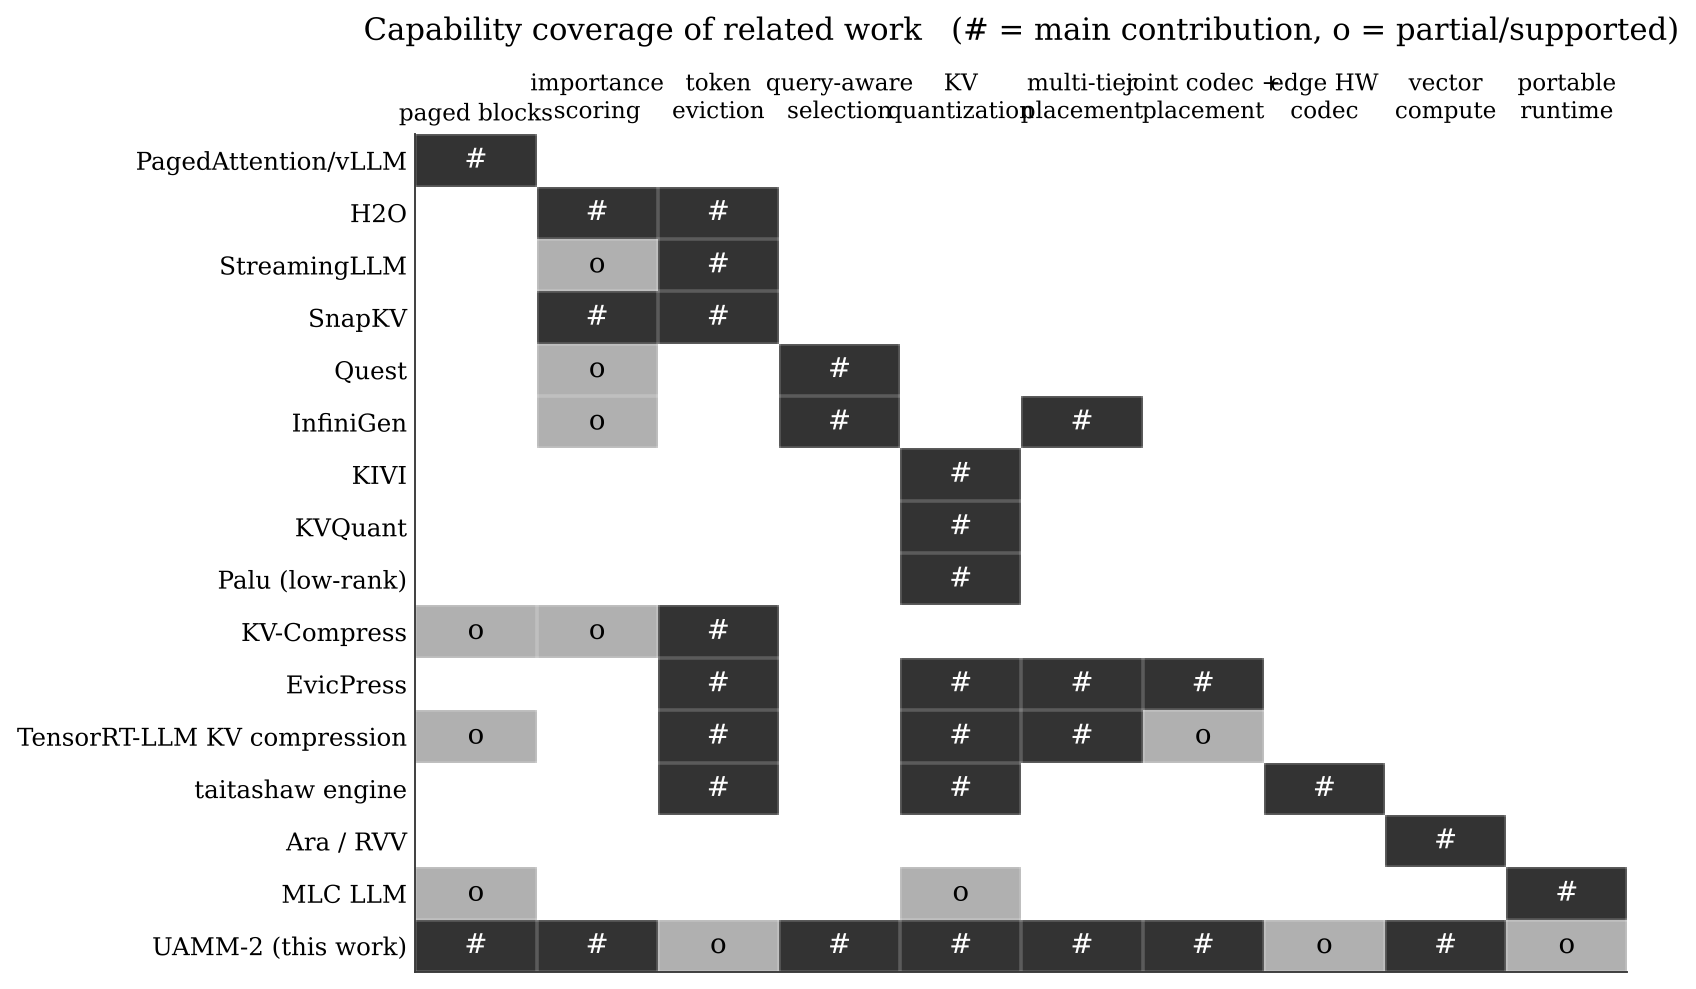
\includegraphics[width=6.27in,height=6.30in,keepaspectratio]{figs/f04_coverage_matrix.png}}
\caption{Capability coverage of the related work. No single prior system covers placement, precision, query-aware selection, importance scoring, a hardware decision engine and a vector kernel together.}
\end{figure}
\section{Summary of the gaps}\label{sec:2_13}
\begin{enumerate}
\item \textbf{Eviction without precision control} (H2O\index{H2O}, Scissorhands\index{Scissorhands}, StreamingLLM\index{StreamingLLM}, SnapKV\index{SnapKV}): loss is irreversible and kept tokens stay at full size.
\item \textbf{Quantisation without selection or placement} (KIVI\index{KIVI}, KVQuant): uniform precision; the whole cache is still read every token.
\item \textbf{Selection without capacity savings} (Quest\index{Quest}): reads fewer bytes but needs everything resident.
\item \textbf{Offloading without compression} (FlexGen, InfiniGen\index{InfiniGen}): one slow tier\index{tier}; no joint precision decision.
\item \textbf{Joint ideas without an edge hardware realisation} (EvicPress\index{EvicPress}, TensorRT-LLM framework): no verified decision hardware, no RISC-V\index{RISC-V} vector path.
\item \textbf{Hardware engines without a policy layer} (compress engines, Ara\index{Ara}): datapaths exist, but nothing decides what to compress and where to put it.
\end{enumerate}
UAMM-2\index{UAMM-2} is an attempt to fill the space between these gaps in one consistent design. The next chapters describe the starting point and the result.

\section{What we learned from each paper and how we used it}\label{sec:11}
This chapter collects, source by source, what we concluded and how it changed the design. Each paper has its own subsection above. Here the lessons are put in one table so that the source of each design decision can be traced. The numbers in square brackets are the entries in the reference list.

{\fontsize{8}{9.5}\selectfont\setlength{\tabcolsep}{3pt}
\begin{longtable}{>{\raggedright\arraybackslash}p{1.40in}>{\raggedright\arraybackslash}p{1.75in}>{\raggedright\arraybackslash}p{1.66in}>{\raggedright\arraybackslash}p{1.05in}}
\caption{Sources, inferences and effects on the design.}\\
\toprule
\textbf{Source} & \textbf{What we learned} & \textbf{How we used it} & \textbf{Not used, and why} \\\midrule\endfirsthead
\toprule \textbf{Source} & \textbf{What we learned} & \textbf{How we used it} & \textbf{Not used, and why} \\\midrule\endhead
\bottomrule\endfoot
PagedAttention / vLLM (SOSP 2023) [1] & Blocks are the right unit; block tables are cheap & Fixed 16-token blocks, block table RTL & Prefix sharing / copy-on-write (open item) \\
H2O (NeurIPS 2023) [2] & Attention is power-law; accumulated attention is a cheap importance signal & Decayed token score → block importance (normalised by p95) & Irreversible eviction as default \\
Scissorhands (NeurIPS 2023) [3] & Importance persists, but can shift & Workload with topic revisits; ability to promote cold blocks & Eviction-only budgeting \\
StreamingLLM (ICLR 2024) [4] & Sink tokens + recent window must be kept & Protected blocks (RTL and Python) & Dropping the middle \\
SnapKV (2024) [5] & A small observation window can seed relevance & Noted as a prefill-time seed (future) & One-shot prompt compression \\
FastGen / PyramidKV [6], [7] & Budgets should differ by head and layer & Structure for future (layer, head) index & Per-head policies (open item) \\
Quest (ICML 2024) [8] & Min/max page summaries give a query-aware bound & Selection by \texttt{Σ max(q·kmin, q·kmax)}; tested as a true bound & Page-level only; no token-level refinement \\
InfiniGen (OSDI 2024) [9] & A slow tier works if the fetch set is predicted & Multi-tier model; planner prices tier latency; prefetch listed as next step & Layer-ahead speculation \\
KIVI (ICML 2024) [10] & Quantise keys per channel and values per token & Codec layer; measured 1.9–5.4× lower key error & Residual full-precision window (we use protected T0 blocks instead) \\
KVQuant (NeurIPS 2024) [11] & Outliers must be handled explicitly; sub-4-bit needs care & Outlier-aware test data; hardware quantiser kept simple & Non-uniform datatypes, pre-RoPE keys (open item) \\
Palu (2024) [12] & Low-rank storage composes with quantisation & Left as a future codec family & Needs model weights \\
FlexGen (ICML 2023) [13] & Placement across tiers can be searched; offload needs compression & Tier + codec search, greedy rather than LP & LP-based optimiser (open item) \\
LLM in a flash [14] & Flash needs large, rare, sequential reads & Flash holds only cold, entropy-capable blocks; large fixed cost per access & Row–column bundling \\
MQA / GQA / MLA [15]–[17] & Architecture changes shrink K/V at training time & Engine accepts any vector size & No model changes \\
EvicPress [24] & Compression and eviction should be decided jointly with a utility & Utility planner (λ-weighted error + latency + congestion) & Our additions: hysteresis, ratchet, query-aware reads, RTL \\
KV-Compress / Zipage [24] & Evict at the paging granularity & Block as unit for every decision & Variable per-head budgets \\
TensorRT-LLM KV compression [24] & Compress when pages change tier & Codec change is part of the same plan step as the move & Vendor-specific kernels \\
CXL-SpecKV [24] & A hardware cache controller can hide slow-memory latency & RTL block table + sweep scorer as controller pieces & CXL fabric \\
Ara / Ara2 [20], [21] & Open RVV vector unit with AXI memory path & Fused QK kernel; codec RTL placed on the load path & Anything run on Ara itself (open item) \\
MLC LLM / TVM-based runtimes [22], [23] & A runtime is an adapter target, not a design dependency & \texttt{RuntimeAdapter} seam; skeleton with checklist & Actual integration (open item) \\
SmoothQuant [19] & Targets weights and activations, not the KV cache & Removed from UAMM-1's list of KV solutions & — \\
Our UAMM-1 (Section~\ref{sec:3}) & Placement without precision cannot fit a tight budget & Ablation baseline; 10 defects fixed & Threshold policy as default \\
\bottomrule
\end{longtable}}
\subsection{Lessons that cut across the papers}
\begin{enumerate}
\item \textbf{Combine axes, not just methods.} The ablation shows that placement alone, codecs alone and eviction alone each leave the budget\index{budget} problem unsolved or solved by loss.
\item \textbf{Measure, do not assume.} Per-block calibrated error is more reliable than a formula; advertised compression ratios are not measured ones.
\item \textbf{Make irreversibility explicit.} The ratchet and opt-in drop make every loss visible and bounded.
\item \textbf{Churn is a first-class cost.} Hysteresis and replanning cadence changed migrations by up to 4× and flash\index{flash} reads by up to 5×.
\item \textbf{Hardware should accelerate the inner loop and be verified like software.} Golden models, boundary vectors and mutation testing\index{mutation testing} found real defects (an ignored \texttt{protected} input, an untested clamp).
\item \textbf{Keep seams.} Codec, runtime and kernel boundaries let each piece be replaced as real measurements arrive.
\end{enumerate}
\chapter{Mind Map of the Project}
The figure on the next page shows the whole project as a sequence of eight steps. Read it left to right and then along the second row. Each step leads to the next one: the problem sent us to the literature, the literature to UAMM-1\index{UAMM-1}, the gaps in UAMM-1 to UAMM-2\index{UAMM-2}, and the results to the open questions in the future scope. The section numbers under each step say where to find the details.

\begin{figure}[htbp]
\centering
\adjustbox{max width=\linewidth}{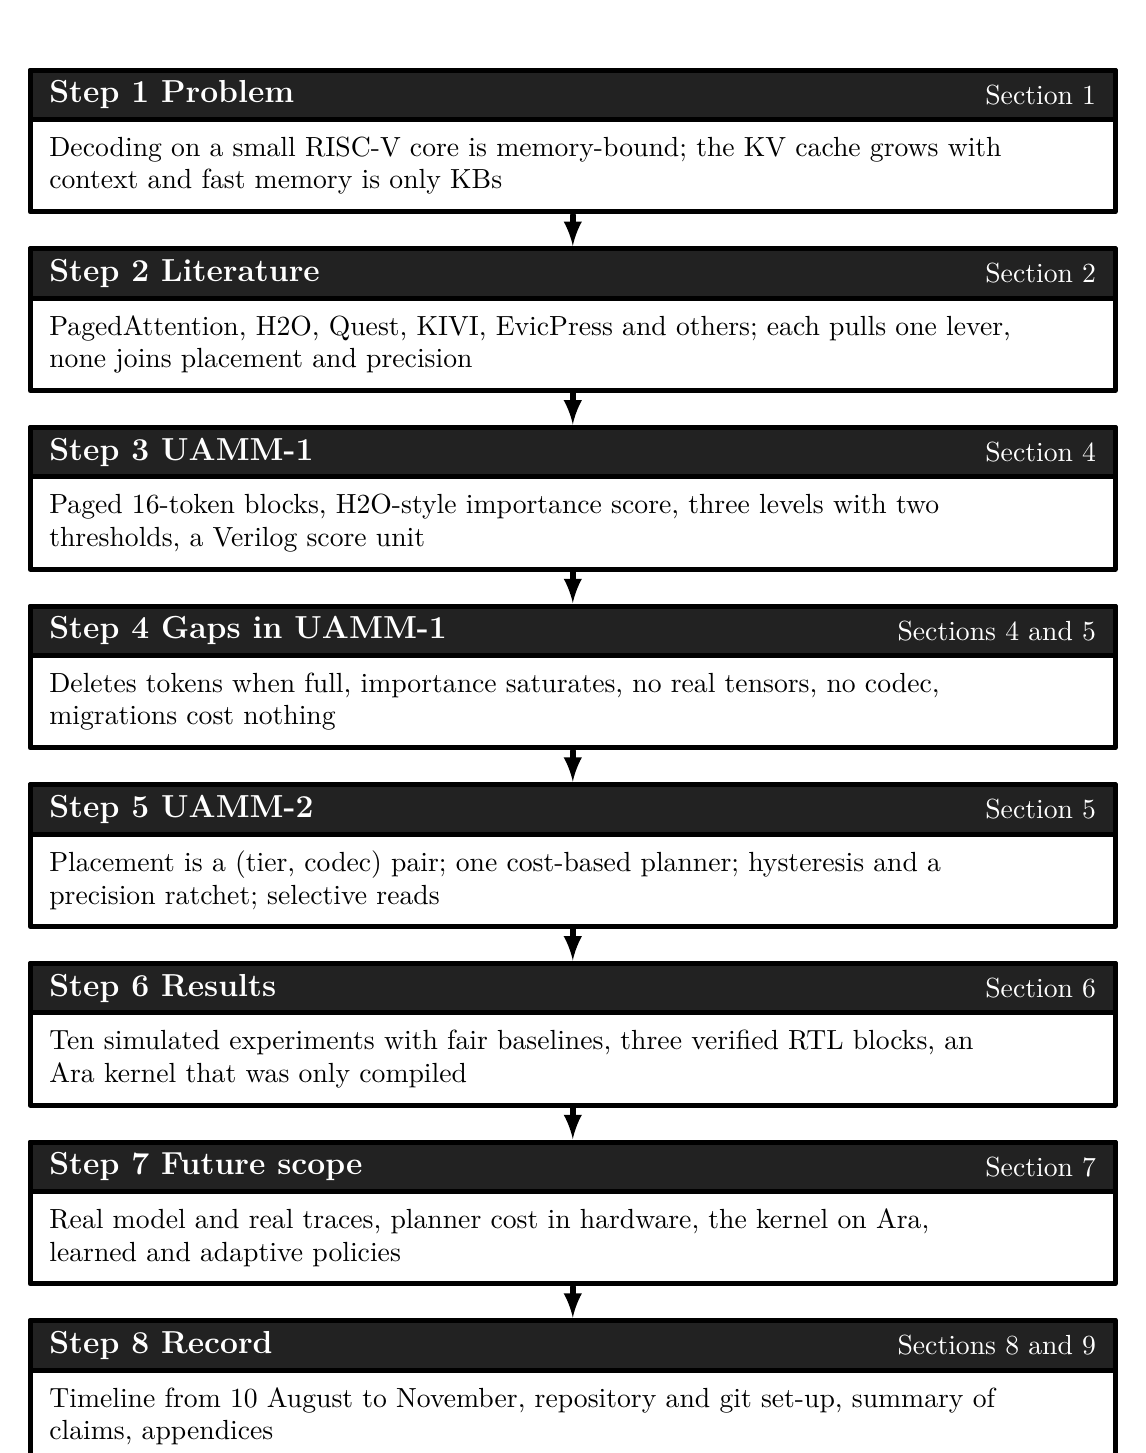
\begin{tikzpicture}[line cap=round,line join=round]
\draw[line width=1.82pt,draw={rgb,255:red,0;green,0;blue,0},fill={rgb,255:red,255;green,255;blue,255}] (0.155in,6.453in) rectangle (5.580in,7.161in);
\draw[line width=1.82pt,draw={rgb,255:red,0;green,0;blue,0},fill={rgb,255:red,34;green,34;blue,34}] (0.155in,6.915in) rectangle (5.580in,7.161in);
\draw[line width=1.82pt,draw={rgb,255:red,0;green,0;blue,0},fill={rgb,255:red,255;green,255;blue,255}] (0.155in,5.559in) rectangle (5.580in,6.268in);
\draw[line width=1.82pt,draw={rgb,255:red,0;green,0;blue,0},fill={rgb,255:red,34;green,34;blue,34}] (0.155in,6.021in) rectangle (5.580in,6.268in);
\draw[line width=1.82pt,draw={rgb,255:red,0;green,0;blue,0},fill={rgb,255:red,255;green,255;blue,255}] (0.155in,4.666in) rectangle (5.580in,5.375in);
\draw[line width=1.82pt,draw={rgb,255:red,0;green,0;blue,0},fill={rgb,255:red,34;green,34;blue,34}] (0.155in,5.128in) rectangle (5.580in,5.375in);
\draw[line width=1.82pt,draw={rgb,255:red,0;green,0;blue,0},fill={rgb,255:red,255;green,255;blue,255}] (0.155in,3.773in) rectangle (5.580in,4.481in);
\draw[line width=1.82pt,draw={rgb,255:red,0;green,0;blue,0},fill={rgb,255:red,34;green,34;blue,34}] (0.155in,4.235in) rectangle (5.580in,4.481in);
\draw[line width=1.82pt,draw={rgb,255:red,0;green,0;blue,0},fill={rgb,255:red,255;green,255;blue,255}] (0.155in,2.880in) rectangle (5.580in,3.588in);
\draw[line width=1.82pt,draw={rgb,255:red,0;green,0;blue,0},fill={rgb,255:red,34;green,34;blue,34}] (0.155in,3.342in) rectangle (5.580in,3.588in);
\draw[line width=1.82pt,draw={rgb,255:red,0;green,0;blue,0},fill={rgb,255:red,255;green,255;blue,255}] (0.155in,1.987in) rectangle (5.580in,2.695in);
\draw[line width=1.82pt,draw={rgb,255:red,0;green,0;blue,0},fill={rgb,255:red,34;green,34;blue,34}] (0.155in,2.449in) rectangle (5.580in,2.695in);
\draw[line width=1.82pt,draw={rgb,255:red,0;green,0;blue,0},fill={rgb,255:red,255;green,255;blue,255}] (0.155in,1.093in) rectangle (5.580in,1.802in);
\draw[line width=1.82pt,draw={rgb,255:red,0;green,0;blue,0},fill={rgb,255:red,34;green,34;blue,34}] (0.155in,1.555in) rectangle (5.580in,1.802in);
\draw[line width=1.82pt,draw={rgb,255:red,0;green,0;blue,0},fill={rgb,255:red,255;green,255;blue,255}] (0.155in,0.200in) rectangle (5.580in,0.909in);
\draw[line width=1.82pt,draw={rgb,255:red,0;green,0;blue,0},fill={rgb,255:red,34;green,34;blue,34}] (0.155in,0.662in) rectangle (5.580in,0.909in);
\node[anchor=west,align=left,text={rgb,255:red,255;green,255;blue,255},font=\fontsize{11.5pt}{13.6pt}\selectfont\bfseries,inner sep=0pt] at (0.248in,7.038in) {Step 1   Problem};
\node[anchor=east,align=right,text={rgb,255:red,255;green,255;blue,255},font=\fontsize{10.0pt}{11.8pt}\selectfont,inner sep=0pt] at (5.487in,7.038in) {Section 1};
\node[anchor=west,align=left,text={rgb,255:red,0;green,0;blue,0},font=\fontsize{10.0pt}{11.8pt}\selectfont,inner sep=0pt] at (0.248in,6.684in) {Decoding on a small RISC-V core is memory-bound; the KV cache grows with \\ context and fast memory is only KBs};
\draw[-latex,line width=2.00pt,draw={rgb,255:red,0;green,0;blue,0}] (2.868in,6.437in) -- (2.868in,6.283in);
\node[anchor=west,align=left,text={rgb,255:red,255;green,255;blue,255},font=\fontsize{11.5pt}{13.6pt}\selectfont\bfseries,inner sep=0pt] at (0.248in,6.145in) {Step 2   Literature};
\node[anchor=east,align=right,text={rgb,255:red,255;green,255;blue,255},font=\fontsize{10.0pt}{11.8pt}\selectfont,inner sep=0pt] at (5.487in,6.145in) {Section 2};
\node[anchor=west,align=left,text={rgb,255:red,0;green,0;blue,0},font=\fontsize{10.0pt}{11.8pt}\selectfont,inner sep=0pt] at (0.248in,5.790in) {PagedAttention, H2O, Quest, KIVI, EvicPress and others; each pulls one lever, \\ none joins placement and precision};
\draw[-latex,line width=2.00pt,draw={rgb,255:red,0;green,0;blue,0}] (2.868in,5.544in) -- (2.868in,5.390in);
\node[anchor=west,align=left,text={rgb,255:red,255;green,255;blue,255},font=\fontsize{11.5pt}{13.6pt}\selectfont\bfseries,inner sep=0pt] at (0.248in,5.251in) {Step 3   UAMM-1};
\node[anchor=east,align=right,text={rgb,255:red,255;green,255;blue,255},font=\fontsize{10.0pt}{11.8pt}\selectfont,inner sep=0pt] at (5.487in,5.251in) {Section 4};
\node[anchor=west,align=left,text={rgb,255:red,0;green,0;blue,0},font=\fontsize{10.0pt}{11.8pt}\selectfont,inner sep=0pt] at (0.248in,4.897in) {Paged 16-token blocks, H2O-style importance score, three levels with two \\ thresholds, a Verilog score unit};
\draw[-latex,line width=2.00pt,draw={rgb,255:red,0;green,0;blue,0}] (2.868in,4.651in) -- (2.868in,4.497in);
\node[anchor=west,align=left,text={rgb,255:red,255;green,255;blue,255},font=\fontsize{11.5pt}{13.6pt}\selectfont\bfseries,inner sep=0pt] at (0.248in,4.358in) {Step 4   Gaps in UAMM-1};
\node[anchor=east,align=right,text={rgb,255:red,255;green,255;blue,255},font=\fontsize{10.0pt}{11.8pt}\selectfont,inner sep=0pt] at (5.487in,4.358in) {Sections 4 and 5};
\node[anchor=west,align=left,text={rgb,255:red,0;green,0;blue,0},font=\fontsize{10.0pt}{11.8pt}\selectfont,inner sep=0pt] at (0.248in,4.004in) {Deletes tokens when full, importance saturates, no real tensors, no codec, \\ migrations cost nothing};
\draw[-latex,line width=2.00pt,draw={rgb,255:red,0;green,0;blue,0}] (2.868in,3.758in) -- (2.868in,3.604in);
\node[anchor=west,align=left,text={rgb,255:red,255;green,255;blue,255},font=\fontsize{11.5pt}{13.6pt}\selectfont\bfseries,inner sep=0pt] at (0.248in,3.465in) {Step 5   UAMM-2};
\node[anchor=east,align=right,text={rgb,255:red,255;green,255;blue,255},font=\fontsize{10.0pt}{11.8pt}\selectfont,inner sep=0pt] at (5.487in,3.465in) {Section 5};
\node[anchor=west,align=left,text={rgb,255:red,0;green,0;blue,0},font=\fontsize{10.0pt}{11.8pt}\selectfont,inner sep=0pt] at (0.248in,3.111in) {Placement is a (tier, codec) pair; one cost-based planner; hysteresis and a \\ precision ratchet; selective reads};
\draw[-latex,line width=2.00pt,draw={rgb,255:red,0;green,0;blue,0}] (2.868in,2.864in) -- (2.868in,2.710in);
\node[anchor=west,align=left,text={rgb,255:red,255;green,255;blue,255},font=\fontsize{11.5pt}{13.6pt}\selectfont\bfseries,inner sep=0pt] at (0.248in,2.572in) {Step 6   Results};
\node[anchor=east,align=right,text={rgb,255:red,255;green,255;blue,255},font=\fontsize{10.0pt}{11.8pt}\selectfont,inner sep=0pt] at (5.487in,2.572in) {Section 6};
\node[anchor=west,align=left,text={rgb,255:red,0;green,0;blue,0},font=\fontsize{10.0pt}{11.8pt}\selectfont,inner sep=0pt] at (0.248in,2.218in) {Ten simulated experiments with fair baselines, three verified RTL blocks, an \\ Ara kernel that was only compiled};
\draw[-latex,line width=2.00pt,draw={rgb,255:red,0;green,0;blue,0}] (2.868in,1.971in) -- (2.868in,1.817in);
\node[anchor=west,align=left,text={rgb,255:red,255;green,255;blue,255},font=\fontsize{11.5pt}{13.6pt}\selectfont\bfseries,inner sep=0pt] at (0.248in,1.679in) {Step 7   Future scope};
\node[anchor=east,align=right,text={rgb,255:red,255;green,255;blue,255},font=\fontsize{10.0pt}{11.8pt}\selectfont,inner sep=0pt] at (5.487in,1.679in) {Section 7};
\node[anchor=west,align=left,text={rgb,255:red,0;green,0;blue,0},font=\fontsize{10.0pt}{11.8pt}\selectfont,inner sep=0pt] at (0.248in,1.324in) {Real model and real traces, planner cost in hardware, the kernel on Ara, \\ learned and adaptive policies};
\draw[-latex,line width=2.00pt,draw={rgb,255:red,0;green,0;blue,0}] (2.868in,1.078in) -- (2.868in,0.924in);
\node[anchor=west,align=left,text={rgb,255:red,255;green,255;blue,255},font=\fontsize{11.5pt}{13.6pt}\selectfont\bfseries,inner sep=0pt] at (0.248in,0.785in) {Step 8   Record};
\node[anchor=east,align=right,text={rgb,255:red,255;green,255;blue,255},font=\fontsize{10.0pt}{11.8pt}\selectfont,inner sep=0pt] at (5.487in,0.785in) {Sections 8 and 9};
\node[anchor=west,align=left,text={rgb,255:red,0;green,0;blue,0},font=\fontsize{10.0pt}{11.8pt}\selectfont,inner sep=0pt] at (0.248in,0.431in) {Timeline from 10 August to November, repository and git set-up, summary of \\ claims, appendices};
\end{tikzpicture}
}
\caption{Mind map of the project, step by step.}
\end{figure}
\chapter{UAMM-1: Our First Prototype}
This section covers UAMM-1\index{UAMM-1} from the beginning: how we reached the problem, what we noticed in existing work, what UAMM-1 is, what we found missing in it, and the code we wrote.

\section{How we arrived at the problem}
We did not start with the KV cache\index{KV cache}. Our first idea was about the processor itself: edge RISC-V\index{RISC-V} cores have vector extensions and address-generation units, and we wanted to see whether better address generation could speed up language-model inference. To judge that, we had to find out where the time actually goes when a language model decodes one token on a small core.

The answer was not what we expected. The multiply-accumulate units are rarely the limit. The core spends most of its time computing addresses, walking tables, unpacking compressed data and waiting for data to arrive from slow memory. Each new token needs the keys and values of every earlier token, and those do not fit in the fast memory next to the processor. The arithmetic is cheap; the memory traffic is not. That moved our attention from the instruction set to the KV cache\index{KV cache} and to the question of where each part of it should live.

The first draft of this paper, submitted on 24 August 2026, was therefore a study of the problem: why generative inference on constrained RISC-V\index{RISC-V} platforms is limited by memory and what a memory manager for it would have to do. This report keeps that analysis as its first chapter and adds what we built afterwards.

\section{What we saw in the existing work}
After the problem was clear, we read the papers (Chapter~2 has the details). What we noticed first was that every method pulls one lever. Paging removes wasted capacity, eviction keeps fewer tokens, selection reads fewer blocks, quantisation\index{quantisation} stores fewer bits and offloading uses slower memory. Each one helps, and each one leaves the other dimensions alone. We could not find a system that treats where a block lives and how many bits it uses as a single decision.

We also noticed that most of this work is written for GPU servers. On an edge processor the fast memory is measured in kilobytes, flash\index{flash} is a real tier\index{tier} and decoding the data competes with the model for the same few cores. So we thought a design built around those limits was worth trying.

Our plan was simple. First build something small that joins the ideas we understood best, see where it breaks, and then fix what breaks. That small thing became UAMM-1\index{UAMM-1}.

\section{First Approach: UAMM-1}\label{sec:3}
Having surveyed the algorithms of Chapter~\ref{sec:2}, we observed that each solves one part of the problem in isolation: paging manages layout, H2O\index{H2O} scores token importance, quantisation\index{quantisation} shrinks tensors, and selection skips reads. The first system we built, \textbf{UAMM-1\index{UAMM-1}} (Unified Adaptive Memory Manager, version 1), was an attempt to join the first two into one memory manager for an edge processor. This chapter describes everything UAMM-1 contained.

\subsection{Components}\label{sec:3_1}
\subsubsection{Paged block store}\label{sec:3_1_1}
The KV cache\index{KV cache} was divided into fixed-size blocks of consecutive tokens, as in PagedAttention\index{PagedAttention}. A block table\index{block table} recorded, for each logical block, the memory level that held it. A block was the unit of allocation, movement and scoring; per-token bookkeeping was avoided.

\subsubsection{H2O-style importance}\label{sec:3_1_2}
Following H2O\index{H2O}, each token accumulated the attention weight it received at every decode step. The importance of a block was a function of the accumulated weights of its tokens. The idea is that a small set of heavy-hitter tokens receives most of the attention, so blocks containing them should be kept close to the processor.

\subsubsection{Three-level placement}\label{sec:3_1_3}
Three memory levels were modelled: a fast level near the processor, DRAM and a slow non-volatile level (flash\index{flash}). Each block received a combined score from three signals:

\begin{center}\small\textit{score = 0.60 · importance + 0.25 · recency + 0.15 · access frequency}\end{center}
and was assigned a level by two fixed thresholds: a block with score ≥ 0.68 went to the fast level, a block with 0.35 ≤ score < 0.68 to DRAM, and a block below 0.35 to flash\index{flash}. When a level was full the block was pushed down to the next level (cascade demotion); when no level had room, the block was discarded.

\begin{calloutbox}{Worked example}
A block has importance 0.90, recency 0.50 and access frequency 0.40. Score = 0.60 × 0.90 + 0.25 × 0.50 + 0.15 × 0.40 = 0.54 + 0.125 + 0.06 = 0.725. Since 0.725 ≥ 0.68 it is placed in the fast level.

A second block has importance 0.20, recency 0.30 and frequency 0.10: score = 0.12 + 0.075 + 0.015 = 0.21 < 0.35, so it goes to flash\index{flash}. If flash is also full, the block is dropped.

\end{calloutbox}
\subsubsection{Hardware decision engine}\label{sec:3_1_4}
A small Verilog module computed the weighted score and the level decision for one block at a time, intended to offload the arithmetic from the processor. It was checked by a testbench with three input vectors.

\subsubsection{Software model}\label{sec:3_1_5}
A Python simulator reproduced the policy, advanced the H2O\index{H2O} scores token by token, and estimated latency from the level each block resided in.

\subsection{What UAMM-1 achieved}\label{sec:3_2}
UAMM-1\index{UAMM-1} showed that importance-driven tiering is workable: hot blocks stay near the processor, cold ones move away, and the decision can be made cheaply in hardware. It also supplied the structure that UAMM-2\index{UAMM-2} keeps: blocks, a block table\index{block table}, a hot/warm/cold classifier and its RTL scorer. For this reason the original threshold policy was retained in the code as a baseline\index{baseline} (\texttt{ThresholdPlanner}), so that UAMM-1 and UAMM-2 can be compared on identical inputs.

\section{Gaps in UAMM-1}\label{sec:4}
Combining paging and importance scoring was a first step, but UAMM-1\index{UAMM-1} inherited the limits of the algorithms it combined and added defects of its own. This chapter identifies each gap, first at the level of ideas and then at the level of implementation, and gives the evidence for its consequence.

\subsection{Gaps at the level of ideas}\label{sec:4_1}
{\fontsize{8}{9.5}\selectfont\setlength{\tabcolsep}{3pt}
\begin{longtable}{>{\raggedright\arraybackslash}p{1.25in}>{\raggedright\arraybackslash}p{2.94in}>{\raggedright\arraybackslash}p{1.78in}}
\caption{Gaps at the level of ideas.}\\
\toprule
\textbf{Gap} & \textbf{Explanation} & \textbf{Consequence} \\\midrule\endfirsthead
\toprule \textbf{Gap} & \textbf{Explanation} & \textbf{Consequence} \\\midrule\endhead
\bottomrule\endfoot
No quantisation & H2O-style importance only decides where a block lives or whether it is deleted. Kept data stays at full 16-bit precision. Quantisation methods such as KIVI, which would shrink kept data, were not part of the system. & When the budget is smaller than the FP16 data, the only remedy is deletion \\
Placement without precision & Importance and placement were linked, but placement and precision were not. A block could not be stored smaller in a slower level. & Slow levels hold full-size blocks and are quickly exhausted \\
No selective reading & All retained blocks were assumed to be read at every step. There was no query-aware rule, as in Quest, for skipping blocks that cannot matter. & Bandwidth stays proportional to the retained cache \\
No measure of codec loss & Because no codec existed, nothing estimated how much error a smaller format would cause for a given block. & No principled trade-off between size and accuracy \\
Irreversible, silent loss & Deletion happened whenever the lowest level was full, without a flag or an opt-in. & Output quality degraded with no visible signal \\
Isolated hardware & The decision engine scored one block at a time and had no memory of block metadata or a translation table. & The software could not hand a whole table to the hardware \\
\bottomrule
\end{longtable}}
\subsection{Defects in the implementation}\label{sec:4_2}
{\fontsize{8}{9.5}\selectfont\setlength{\tabcolsep}{3pt}
\begin{longtable}{>{\raggedright\arraybackslash}p{2.05in}>{\raggedright\arraybackslash}p{1.69in}>{\raggedright\arraybackslash}p{2.23in}}
\caption{Implementation defects found on review and the response to each.}\\
\toprule
\textbf{Defect} & \textbf{Why it matters} & \textbf{Response in UAMM-2} \\\midrule\endfirsthead
\toprule \textbf{Defect} & \textbf{Why it matters} & \textbf{Response in UAMM-2} \\\midrule\endhead
\bottomrule\endfoot
The eviction decision was computed but never acted on, and data was deleted silently when the lowest level was full & Output changes without notice & Drop is explicit and opt-in; otherwise overflow is reported as a number \\
Importance was clamped at 1.0 although H2O scores are sums that grow without bound & Heavy hitters and sinks saturate; the signal stops discriminating & Scores decay each step; block importance is normalised by the 95th percentile \\
Recency was constant or unused & A quarter of the score carried no information & Recency enters through an exponential average of how often attention fetched the block \\
No capacity-aware cascade and no hysteresis & Blocks oscillate between levels; each move costs energy & Greedy capacity-aware assignment, minimum residency and a relative-improvement margin \\
Latency charged per token, migrations free & Cost of moving data was invisible & Cost per block per level and codec; migrations accounted separately \\
O(N) Python loop per token for H2O & Does not scale with context & One vectorised decay per step \\
Division by 100 in Verilog & Dividers are large and slow & Integer weights 154/64/38 (sum 256) and a shift \\
Verilog and Python disagreed on protected blocks & Hardware and software make different decisions & RTL honours the protected flag; bit-exact golden model \\
Three test vectors, no boundary cases & Little confidence in the RTL & 17 sweeps with threshold edges, 400 codec vectors, 6,000 random table operations, mutation testing \\
SmoothQuant listed as a KV-cache solution & It targets weights and activations & Replaced by KV-specific KIVI-style codecs \\
\bottomrule
\end{longtable}}
\subsection{Evidence: what the gaps cost}\label{sec:4_3}
The experiments of Section~\ref{sec:8} measure the consequence. With a total budget\index{budget} of 168 KB for 1,536 tokens (FP16\index{FP16} would need 393 KB), the UAMM-1\index{UAMM-1} policy keeps 0.37 of the FP16 footprint only by permanently deleting 973 of the 1,536 tokens on average. The remaining blocks then retain only 0.76 of the attention mass, the mean relative error of the attention output is 0.48, and about 12,613 block reads are served from flash\index{flash}. A system with codecs, by contrast, keeps every token at 0.31 of the FP16 footprint with 0.94 recall\index{recall}. The gap is therefore not in the placement rule but in the absence of a way to make data smaller and of a way to read less.

\begin{calloutbox}{Summary of what was left unresolved}
1. No quantisation\index{quantisation}, so a tight budget\index{budget} forces deletion.

2. Placement and precision decided separately (placement only).

3. No query-aware selection of what to read.

4. No measured error per block, hence no principled quality control.

5. Silent, irreversible loss and several implementation defects.

6. Hardware that was neither connected to a block table\index{block table} nor adequately verified.

\end{calloutbox}
\section{Implementing UAMM-1: the code, how to run it and where the data comes from}
\subsection{What we wrote}
UAMM-1\index{UAMM-1} is a small Python simulator with one Verilog module. It does not run a language model. It models only the \textit{bookkeeping} of a KV cache\index{KV cache}: which block is where, how much attention each token received and what a read from each memory level would cost. The files are listed in the table below.

{\fontsize{8}{9.5}\selectfont\setlength{\tabcolsep}{3pt}
\begin{longtable}{>{\raggedright\arraybackslash}p{1.25in}>{\raggedright\arraybackslash}p{4.81in}}
\caption{The files of UAMM-1.}\\
\toprule
\textbf{File} & \textbf{What it contains} \\\midrule\endfirsthead
\toprule \textbf{File} & \textbf{What it contains} \\\midrule\endhead
\bottomrule\endfoot
\texttt{config.\allowbreak{}py} & Block size (16 tokens), capacities of the three levels in blocks (8, 16, 64), the weights 0.60/0.25/0.15, the thresholds 0.68 and 0.35, the recent window (32 tokens) and three assumed read times \\
\texttt{paged\_\allowbreak{}\allowbreak{}cache.\allowbreak{}py} & \texttt{KVBlock} (importance, recency, access count, protected flag) and \texttt{PagedKVCache}, which appends tokens and opens a new block every 16 tokens \\
\texttt{h2o.\allowbreak{}py} & \texttt{H2OImportanceTracker}: adds the attention a token received to the token's running score and sums it up per block \\
\texttt{controller.\allowbreak{}py} & \texttt{UnifiedMemoryController}: computes the weighted score of a block and returns a target level and an evict flag \\
\texttt{memory\_\allowbreak{}\allowbreak{}tiers.\allowbreak{}py} & \texttt{MemoryTiers}: counts blocks in each level, enforces capacity, counts transfers and evictions \\
\texttt{simulator.\allowbreak{}py} & \texttt{UAMMSimulator}: the per-token loop that ties the above together, and a \texttt{Metrics} summary \\
\texttt{cli.\allowbreak{}py} & Command line: \texttt{--tokens}, \texttt{--block-size}, \texttt{--gpu-blocks}, \texttt{--cpu-blocks}, \texttt{--nvme-blocks} \\
Verilog & \texttt{uamm\_\allowbreak{}\allowbreak{}controller}: computes the same score for one block and outputs a level and an evict flag; with a testbench of three vectors \\
\bottomrule
\end{longtable}}
\subsection{What it does at every token}
\begin{enumerate}
\item Append the token to the cache. If the last block is full, open a new one and place it in the fastest level.
\item Create a simulated attention vector over the recent tokens (see below) and let the H2O\index{H2O} tracker add it to the token scores.
\item Mark every block that holds one of the last 32 tokens as protected, and update each block's recency.
\item Charge a read time for every block that the attention touched, depending on the level the block is in.
\item For every block compute \texttt{0.\allowbreak{}60·importance + 0.\allowbreak{}25·recency + 0.\allowbreak{}15·frequency} and compare it with the two thresholds. Move the block to the level the score selects, pushing the least valuable block down when that level is full.
\item At the end report the simulated first-token time, inter-token time, throughput, peak use of the fast level, number of transfers and number of evictions.
\end{enumerate}
\subsection{How to run it}
From the folder that holds the UAMM-1\index{UAMM-1} package, run the command-line module with the number of tokens and, if you want to change them, the capacities of the three levels:

\par\smallskip\noindent\textbf{Running UAMM-1}\par\nopagebreak
\begin{lstlisting}
python3 -m <package>.cli --tokens 512 --block-size 16 --gpu-blocks 8 --cpu-blocks 16 --nvme-blocks 64
\end{lstlisting}
The program prints the number of blocks in each level and the metrics dictionary. The Verilog testbench is run with any Verilog simulator (we used Verilator\index{Verilator}). The complete source is in the appendix on the original prototype, and a copy of the listing is in \texttt{uamm1\_\allowbreak{}\allowbreak{}original/\allowbreak{}} in the repository.

\subsection{Where its data points come from}
UAMM-1\index{UAMM-1} has no input data in the usual sense. At each token the simulator \textit{invents} an attention vector: a random number between 0 and 1 for each of the last eight tokens, a random number scaled by 0.15 for the older tokens in the recent window, and a constant boost of 0.8 for token 0, which plays the part of an attention sink\index{attention sink}. The random generator is seeded with 7, so a run is repeatable. The read times (0.02 ms, 0.20 ms and 4.0 ms for the three levels) are numbers we assumed, not measured. The metrics are therefore outputs of a model with made-up inputs, and we only used them to compare policies with each other. We did not obtain any value from a real language model.

\begin{calloutbox}{What this tells us about UAMM-1}
UAMM-1\index{UAMM-1} let us check that an importance-driven placement runs end to end and that the scoring logic can sit in hardware. It could not tell us how much accuracy a policy loses, because it never held real key and value vectors. This was the first thing we changed in UAMM-2\index{UAMM-2}: the cache now stores real tensors and attention is computed on them.

\end{calloutbox}
\subsection{The scoring code, line by line}
The decision for one block is made in \texttt{UnifiedMemoryController} (\texttt{controller.\allowbreak{}py}). The listing below is the core of it, unchanged from the prototype. \texttt{score} turns three numbers into one: the block's importance from the H2O\index{H2O} tracker, how recently it was used, and how often it was used. Each is scaled to the range 0 to 1 before the weights \texttt{alpha}, \texttt{beta} and \texttt{gamma} (0.60, 0.25 and 0.15) are applied. \texttt{decide} then compares the score with two thresholds and picks the level. A block is also marked for eviction when the lowest level is nearly full (pressure at least 0.95), its score is below the lower threshold and it is not protected.

\par\smallskip\noindent\textbf{UAMM-1 controller: score and decide (controller.py)}\par\nopagebreak
\begin{lstlisting}
class UnifiedMemoryController:
    def __init__(self, config: Config):
        self.cfg = config

    @staticmethod
    def _norm(value: float, maximum: float) -> float:
        return max(0.0, min(1.0, value / maximum if maximum > 0 else 0.0))

    def score(self, block: KVBlock, now: int, max_age: int, max_frequency: int) -> float:
        importance = self._norm(block.importance, 1.0)
        age = max(0, now - block.last_access)
        recency = 1.0 - self._norm(age, max(1, max_age))
        frequency = self._norm(block.access_count, max(1, max_frequency))
        return (self.cfg.alpha * importance +
                self.cfg.beta * recency +
                self.cfg.gamma * frequency)

    def decide(self, block: KVBlock, now: int, max_age: int, max_frequency: int,
               pressure: float) -> Decision:
        score = self.score(block, now, max_age, max_frequency)
        if score >= self.cfg.gpu_threshold:
            tier = "gpu"
        elif score >= self.cfg.cpu_threshold:
            tier = "cpu"
        else:
            tier = "nvme"
        evict = pressure >= 0.95 and score < self.cfg.cpu_threshold and not block.protected
        return Decision(score, tier, evict)

from collections import defaultdict
from typing import Dict, Iterable
from .paged_cache import PagedKVCache
\end{lstlisting}
Two things in this code explain the gaps we found later. The importance is clamped to 1.0 by \texttt{\_\allowbreak{}\allowbreak{}norm}, so heavy-hitter blocks all reach the same value. And the only outcomes are a level or an eviction, so there is no way to keep a block in a smaller form.

\subsection{Making room when a level is full}
\texttt{\_\allowbreak{}\allowbreak{}ensure\_\allowbreak{}\allowbreak{}capacity} in \texttt{simulator.\allowbreak{}py} runs whenever a block has to move into a level that has no free slot. It picks the resident block with the lowest importance that is not protected and pushes it one level down. If the bottom level is also full, the victim is removed from the cache altogether, which is the deletion that cost UAMM-1\index{UAMM-1} 973 of 1,536 tokens in our comparison.

\par\smallskip\noindent\textbf{UAMM-1: demoting or deleting a victim block (simulator.py)}\par\nopagebreak
\begin{lstlisting}
      def _ensure_capacity(self, target: str, incoming_id: int):
          if self.tiers.has_space(target):
              return True
          # Demote the least valuable, unprotected resident block to a slower tier.
          candidates = []
          for block_id in self.tiers.blocks[target]:
              b = self.cache.get_block(block_id)
              if not b.protected and block_id != incoming_id:
                  candidates.append((b.importance + b.recency * 0.01, block_id))
          if not candidates:
              return False
          _, victim_id = min(candidates)
          fallback = "cpu" if target == "gpu" else "nvme"
          if fallback == "nvme" and not self.tiers.has_space("nvme"):
              self.tiers.remove(victim_id)
              self.cache.remove_block(victim_id)
\end{lstlisting}
\chapter{UAMM-2: Problems We Found and How We Corrected Them}
This section follows UAMM-2\index{UAMM-2} the way we lived it. For each part of the design we describe what we tried, what we saw when we ran it, what we decided and what we set aside. Some decisions came from an experiment and some from reasoning about the edge processor; we say which. After the decisions we list the problems in the design and in our own results, and then describe the system as it stands and how the code is organised.

\section{The idea behind UAMM-2}
When we went through the gaps in UAMM-1\index{UAMM-1}, most of them could be fixed locally. Deleting data silently, an importance value that saturated and migrations that cost nothing were all bugs of the kind you patch. One gap was different: UAMM-1 could decide \textit{where} a block lived but never \textit{how big} it was. That needed a new structure, and it is what UAMM-2\index{UAMM-2} is built around.

So in UAMM-2\index{UAMM-2} every block has a placement that is a pair, (tier\index{tier}, codec\index{codec}), where the codec is the storage format of the block (we defined the word in Chapter~1). A cold block does not have to be deleted; it can move to a slower tier and be stored in 4 or 2 bits. A hot block can stay in FP16\index{FP16} in the fastest tier. A planner\index{planner} makes the choice for all blocks together by adding up three costs: the time to read and decode the block, a penalty for the error the codec introduces (weighted by how hot the block is), and a price for using scarce capacity. Three rules keep it stable: precision can only go down, blocks must stay put for a minimum time and a move must be a clear improvement, and deletion is switched off unless explicitly requested. Attention then reads only the blocks that can matter for the current query. Chapter~4 describes the design in full.

\section{How UAMM-2 is built}
This part describes the system we ended with: its memory tiers, the block and its life cycle, the codecs, the importance signal, the planner\index{planner}, selective attention\index{selective attention}, the hardware blocks and the vector kernel. The decisions behind each choice, and the problems we met, follow in the next two parts.

\section{The System Design of UAMM-2}\label{sec:5}
The knowledge that went into UAMM-2\index{UAMM-2} comes from the papers in the literature review: blocks from PagedAttention\index{PagedAttention}, the importance signal from H2O\index{H2O}, protected sink and recent tokens from StreamingLLM\index{StreamingLLM}, the query-aware bound from Quest\index{Quest}, the asymmetric quantisation\index{quantisation} of keys and values from KIVI\index{KIVI}, and the idea of deciding compression and eviction together from EvicPress\index{EvicPress}. The rest of this part shows how these were turned into code, hardware and a kernel.

\subsection{The core idea: a placement is a (tier, codec) pair}\label{sec:5_1}
Every block of the KV cache\index{KV cache} is described by two coordinates. The \textbf{tier\index{tier}} says \textit{where} it is stored (and therefore what a read costs). The \textbf{codec\index{codec}} says \textit{how many bits} it occupies (and therefore how big it is and how much error it carries). The planner\index{planner} picks both together. A block that is almost never attended is best stored in flash\index{flash} as a 2-bit entropy-coded blob. A block that is hot but large can stay in DRAM at 4 bits. Protected blocks (sinks, recent window) sit in the fastest tier at full precision. Choosing the two jointly lets the system exchange precision for capacity instead of exchanging data for nothing.

\begin{figure}[htbp]
\centering
\adjustbox{max width=\linewidth}{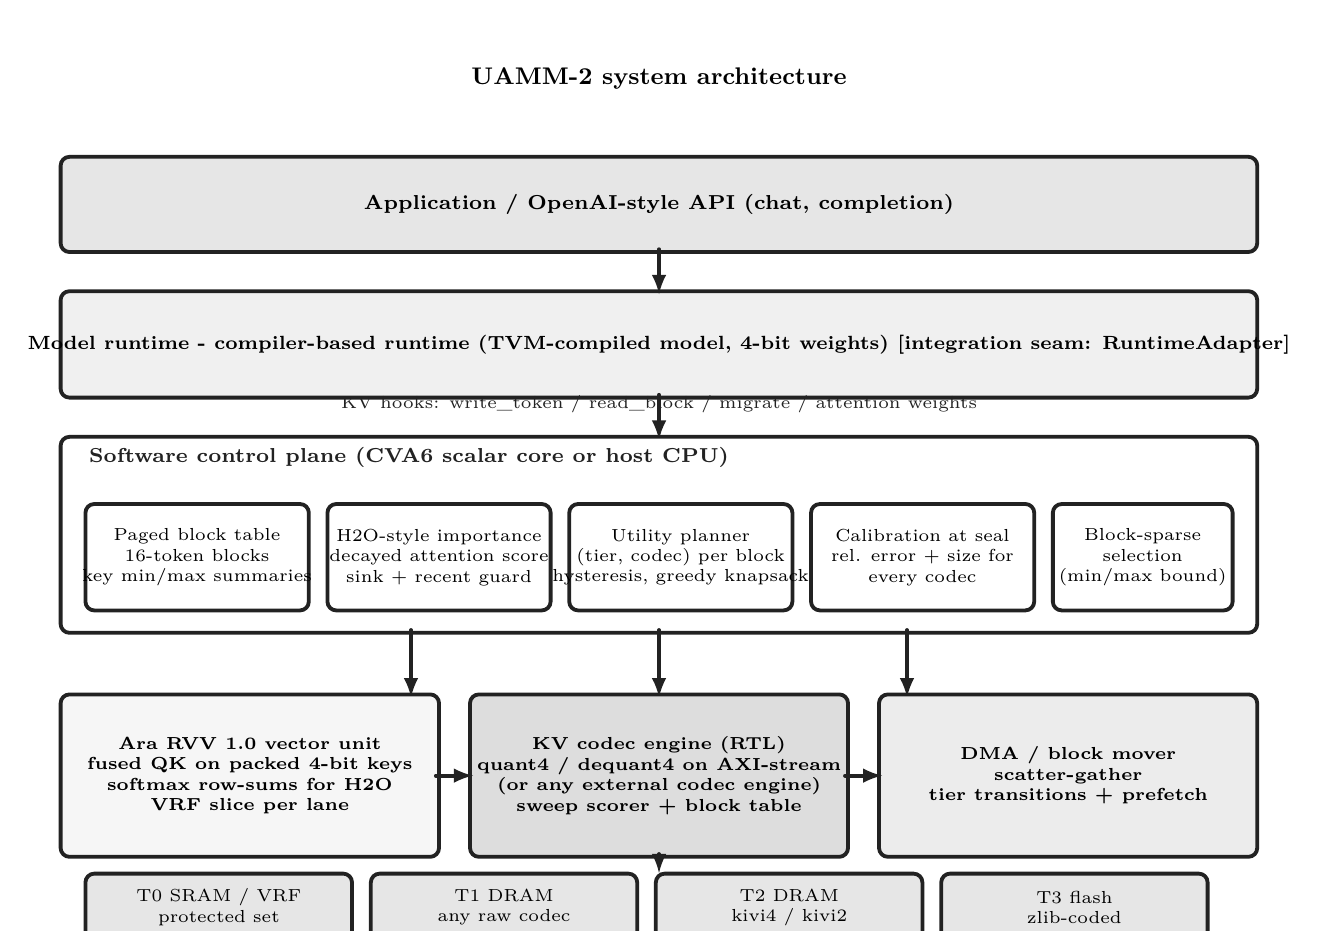
\begin{tikzpicture}[line cap=round,line join=round]
\draw[rounded corners=3.2pt,line width=1.38pt,draw={rgb,255:red,34;green,34;blue,34},fill={rgb,255:red,230;green,230;blue,230}] (0.108in,3.458in) rectangle (6.091in,3.934in);
\draw[rounded corners=3.2pt,line width=1.38pt,draw={rgb,255:red,34;green,34;blue,34},fill={rgb,255:red,240;green,240;blue,240}] (0.108in,2.730in) rectangle (6.091in,3.262in);
\draw[-latex,line width=1.38pt,draw={rgb,255:red,34;green,34;blue,34}] (3.100in,3.472in) -- (3.100in,3.248in);
\draw[-latex,line width=1.38pt,draw={rgb,255:red,34;green,34;blue,34}] (3.100in,2.744in) -- (3.100in,2.520in);
\draw[rounded corners=3.2pt,line width=1.38pt,draw={rgb,255:red,34;green,34;blue,34},fill={rgb,255:red,255;green,255;blue,255}] (0.108in,1.554in) rectangle (6.091in,2.534in);
\draw[rounded corners=3.2pt,line width=1.38pt,draw={rgb,255:red,34;green,34;blue,34},fill={rgb,255:red,255;green,255;blue,255}] (0.232in,1.666in) rectangle (1.349in,2.198in);
\draw[rounded corners=3.2pt,line width=1.38pt,draw={rgb,255:red,34;green,34;blue,34},fill={rgb,255:red,255;green,255;blue,255}] (1.442in,1.666in) rectangle (2.558in,2.198in);
\draw[rounded corners=3.2pt,line width=1.38pt,draw={rgb,255:red,34;green,34;blue,34},fill={rgb,255:red,255;green,255;blue,255}] (2.651in,1.666in) rectangle (3.767in,2.198in);
\draw[rounded corners=3.2pt,line width=1.38pt,draw={rgb,255:red,34;green,34;blue,34},fill={rgb,255:red,255;green,255;blue,255}] (3.860in,1.666in) rectangle (4.976in,2.198in);
\draw[rounded corners=3.2pt,line width=1.38pt,draw={rgb,255:red,34;green,34;blue,34},fill={rgb,255:red,255;green,255;blue,255}] (5.069in,1.666in) rectangle (5.968in,2.198in);
\draw[-latex,line width=1.38pt,draw={rgb,255:red,34;green,34;blue,34}] (1.860in,1.568in) -- (1.860in,1.232in);
\draw[-latex,line width=1.38pt,draw={rgb,255:red,34;green,34;blue,34}] (3.100in,1.568in) -- (3.100in,1.232in);
\draw[-latex,line width=1.38pt,draw={rgb,255:red,34;green,34;blue,34}] (4.340in,1.568in) -- (4.340in,1.232in);
\draw[rounded corners=3.2pt,line width=1.38pt,draw={rgb,255:red,34;green,34;blue,34},fill={rgb,255:red,246;green,246;blue,246}] (0.108in,0.434in) rectangle (2.000in,1.246in);
\draw[rounded corners=3.2pt,line width=1.38pt,draw={rgb,255:red,34;green,34;blue,34},fill={rgb,255:red,221;green,221;blue,221}] (2.155in,0.434in) rectangle (4.045in,1.246in);
\draw[rounded corners=3.2pt,line width=1.38pt,draw={rgb,255:red,34;green,34;blue,34},fill={rgb,255:red,236;green,236;blue,236}] (4.200in,0.434in) rectangle (6.091in,1.246in);
\draw[-latex,line width=1.38pt,draw={rgb,255:red,34;green,34;blue,34}] (1.984in,0.840in) -- (2.170in,0.840in);
\draw[-latex,line width=1.38pt,draw={rgb,255:red,34;green,34;blue,34}] (4.030in,0.840in) -- (4.216in,0.840in);
\draw[rounded corners=3.2pt,line width=1.38pt,draw={rgb,255:red,34;green,34;blue,34},fill={rgb,255:red,230;green,230;blue,230}] (0.232in,0.014in) rectangle (1.565in,0.350in);
\draw[rounded corners=3.2pt,line width=1.38pt,draw={rgb,255:red,34;green,34;blue,34},fill={rgb,255:red,230;green,230;blue,230}] (1.659in,0.014in) rectangle (2.991in,0.350in);
\draw[rounded corners=3.2pt,line width=1.38pt,draw={rgb,255:red,34;green,34;blue,34},fill={rgb,255:red,230;green,230;blue,230}] (3.084in,0.014in) rectangle (4.417in,0.350in);
\draw[rounded corners=3.2pt,line width=1.38pt,draw={rgb,255:red,34;green,34;blue,34},fill={rgb,255:red,230;green,230;blue,230}] (4.511in,0.014in) rectangle (5.843in,0.350in);
\draw[-latex,line width=1.38pt,draw={rgb,255:red,34;green,34;blue,34}] (3.100in,0.448in) -- (3.100in,0.353in);
\node[align=center,text={rgb,255:red,0;green,0;blue,0},font=\fontsize{7.3pt}{8.6pt}\selectfont\bfseries,inner sep=0pt] at (3.100in,3.696in) {Application / OpenAI-style API   (chat, completion)};
\node[align=center,text={rgb,255:red,0;green,0;blue,0},font=\fontsize{6.9pt}{8.2pt}\selectfont\bfseries,inner sep=0pt] at (3.100in,2.996in) {Model runtime  -  compiler-based runtime (TVM-compiled model, 4-bit weights)   [integration seam: RuntimeAdapter]};
\node[align=center,text={rgb,255:red,34;green,34;blue,34},font=\fontsize{6.3pt}{7.4pt}\selectfont,inner sep=0pt] at (3.100in,2.699in) {KV hooks: write\_token / read\_block / migrate / attention weights};
\node[anchor=south west,align=left,text={rgb,255:red,34;green,34;blue,34},font=\fontsize{7.3pt}{8.6pt}\selectfont\bfseries,inner sep=0pt] at (0.248in,2.380in) {Software control plane (CVA6 scalar core or host CPU)};
\node[align=center,text={rgb,255:red,0;green,0;blue,0},font=\fontsize{6.3pt}{7.4pt}\selectfont,inner sep=0pt] at (0.790in,1.932in) {Paged block table \\ 16-token blocks \\ key min/max summaries};
\node[align=center,text={rgb,255:red,0;green,0;blue,0},font=\fontsize{6.3pt}{7.4pt}\selectfont,inner sep=0pt] at (2.000in,1.932in) {H2O-style importance \\ decayed attention score \\ sink + recent guard};
\node[align=center,text={rgb,255:red,0;green,0;blue,0},font=\fontsize{6.3pt}{7.4pt}\selectfont,inner sep=0pt] at (3.208in,1.932in) {Utility planner \\ (tier, codec) per block \\ hysteresis, greedy knapsack};
\node[align=center,text={rgb,255:red,0;green,0;blue,0},font=\fontsize{6.3pt}{7.4pt}\selectfont,inner sep=0pt] at (4.417in,1.932in) {Calibration at seal \\ rel. error + size for \\ every codec};
\node[align=center,text={rgb,255:red,0;green,0;blue,0},font=\fontsize{6.3pt}{7.4pt}\selectfont,inner sep=0pt] at (5.518in,1.932in) {Block-sparse \\ selection \\ (min/max bound)};
\node[align=center,text={rgb,255:red,0;green,0;blue,0},font=\fontsize{6.3pt}{7.4pt}\selectfont\bfseries,inner sep=0pt] at (1.054in,0.840in) {Ara RVV 1.0 vector unit \\ fused QK on packed 4-bit keys \\ softmax row-sums for H2O \\ VRF slice per lane};
\node[align=center,text={rgb,255:red,0;green,0;blue,0},font=\fontsize{6.3pt}{7.4pt}\selectfont\bfseries,inner sep=0pt] at (3.100in,0.840in) {KV codec engine (RTL) \\ quant4 / dequant4 on AXI-stream \\ (or any external codec engine) \\ sweep scorer + block table};
\node[align=center,text={rgb,255:red,0;green,0;blue,0},font=\fontsize{6.3pt}{7.4pt}\selectfont\bfseries,inner sep=0pt] at (5.146in,0.840in) {DMA / block mover \\ scatter-gather \\ tier transitions + prefetch};
\node[align=center,text={rgb,255:red,0;green,0;blue,0},font=\fontsize{6.3pt}{7.4pt}\selectfont,inner sep=0pt] at (0.899in,0.182in) {T0  SRAM / VRF \\ protected set};
\node[align=center,text={rgb,255:red,0;green,0;blue,0},font=\fontsize{6.3pt}{7.4pt}\selectfont,inner sep=0pt] at (2.325in,0.182in) {T1  DRAM \\ any raw codec};
\node[align=center,text={rgb,255:red,0;green,0;blue,0},font=\fontsize{6.3pt}{7.4pt}\selectfont,inner sep=0pt] at (3.751in,0.182in) {T2  DRAM \\ kivi4 / kivi2};
\node[align=center,text={rgb,255:red,0;green,0;blue,0},font=\fontsize{6.3pt}{7.4pt}\selectfont,inner sep=0pt] at (5.177in,0.182in) {T3  flash \\ zlib-coded};
\node[anchor=south,align=center,text={rgb,255:red,0;green,0;blue,0},font=\fontsize{8.7pt}{10.3pt}\selectfont\bfseries,inner sep=0pt] at (3.100in,4.268in) {UAMM-2 system architecture};
\end{tikzpicture}
}
\caption{UAMM-2 system architecture: the decode loop, the paged cache with its tiers and codecs, the importance and planning loop, and the hardware and vector-kernel attachments.}
\end{figure}
\subsection{Memory hierarchy and tiers}\label{sec:5_2}
{\fontsize{8}{9.5}\selectfont\setlength{\tabcolsep}{3pt}
\begin{longtable}{>{\raggedright\arraybackslash}p{0.34in}>{\raggedright\arraybackslash}p{1.20in}>{\raggedright\arraybackslash}p{0.69in}>{\raggedright\arraybackslash}p{1.12in}>{\raggedright\arraybackslash}p{1.12in}>{\raggedright\arraybackslash}p{1.20in}}
\caption{Tiers used in the simulations. Capacities are deliberately small so that the budget is tight at a few thousand tokens; latencies and bandwidths are assumed values (Section~\ref{sec:7}).}\\
\toprule
\textbf{Tier} & \textbf{Where it models} & \textbf{Capacity in experiments} & \textbf{Base latency / bandwidth (assumed)} & \textbf{Allowed codecs} & \textbf{Intended contents} \\\midrule\endfirsthead
\toprule \textbf{Tier} & \textbf{Where it models} & \textbf{Capacity in experiments} & \textbf{Base latency / bandwidth (assumed)} & \textbf{Allowed codecs} & \textbf{Intended contents} \\\midrule\endhead
\bottomrule\endfoot
T0 & Near-compute SRAM / vector register file & 24 KB & 0.5 µs / 100 GB/s & any raw codec & Sink tokens, recent window, unsealed block \\
T1 & DRAM, hot & 48 KB & 2 µs / 12.8 GB/s & any raw (non-entropy) codec & Frequently fetched blocks; also where 2-bit blocks sit if the planner prices them there \\
T2 & DRAM, warm & 32 KB & 2 µs / 12.8 GB/s & kivi4, kivi2 & Occasionally fetched blocks \\
T3 & Flash & 64 KB & 100 µs / 1 GB/s & int8z, kivi4z, kivi2z (entropy-coded) & Cold blocks \\
\bottomrule
\end{longtable}}
\begin{figure}[htbp]
\centering
\adjustbox{max width=\linewidth}{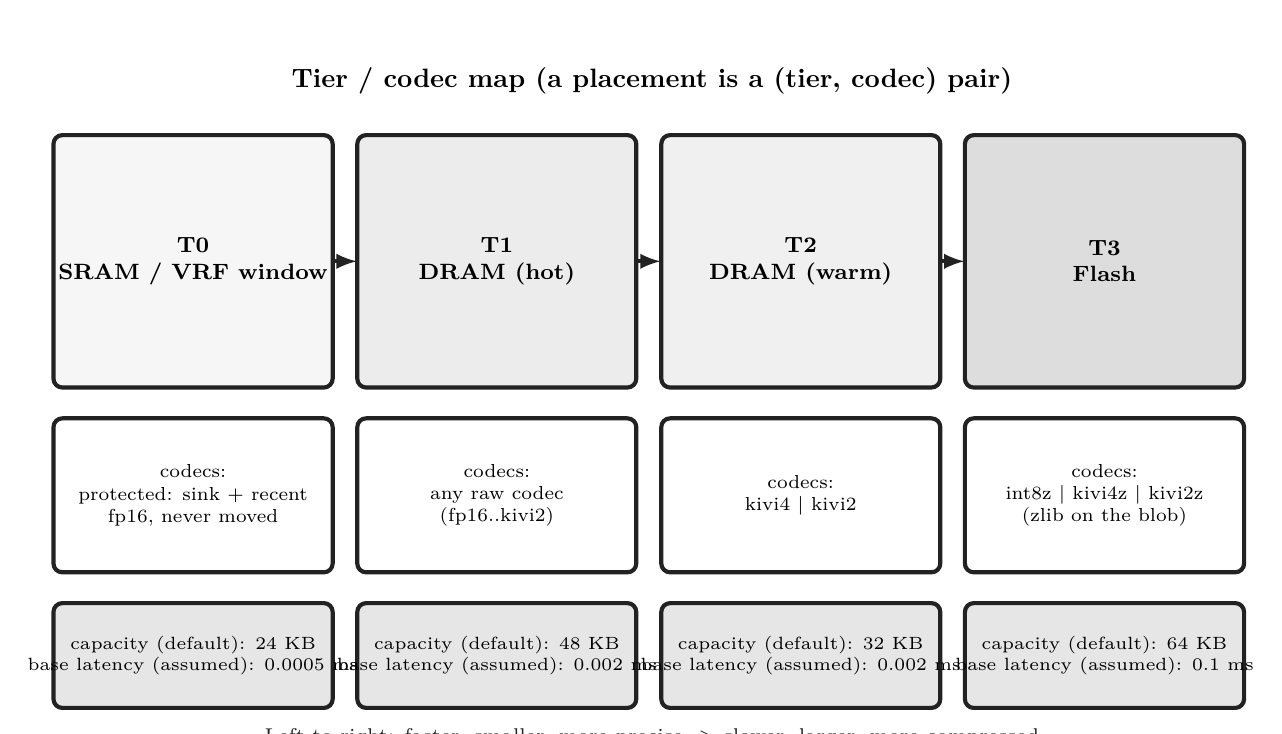
\begin{tikzpicture}[line cap=round,line join=round]
\draw[rounded corners=3.2pt,line width=1.50pt,draw={rgb,255:red,34;green,34;blue,34},fill={rgb,255:red,246;green,246;blue,246}] (0.108in,1.833in) rectangle (1.504in,3.095in);
\draw[rounded corners=3.2pt,line width=1.50pt,draw={rgb,255:red,34;green,34;blue,34},fill={rgb,255:red,255;green,255;blue,255}] (0.108in,0.909in) rectangle (1.504in,1.679in);
\draw[rounded corners=3.2pt,line width=1.50pt,draw={rgb,255:red,34;green,34;blue,34},fill={rgb,255:red,230;green,230;blue,230}] (0.108in,0.231in) rectangle (1.504in,0.755in);
\draw[-latex,line width=1.50pt,draw={rgb,255:red,34;green,34;blue,34}] (1.507in,2.464in) -- (1.624in,2.464in);
\draw[rounded corners=3.2pt,line width=1.50pt,draw={rgb,255:red,34;green,34;blue,34},fill={rgb,255:red,236;green,236;blue,236}] (1.627in,1.833in) rectangle (3.022in,3.095in);
\draw[rounded corners=3.2pt,line width=1.50pt,draw={rgb,255:red,34;green,34;blue,34},fill={rgb,255:red,255;green,255;blue,255}] (1.627in,0.909in) rectangle (3.022in,1.679in);
\draw[rounded corners=3.2pt,line width=1.50pt,draw={rgb,255:red,34;green,34;blue,34},fill={rgb,255:red,230;green,230;blue,230}] (1.627in,0.231in) rectangle (3.022in,0.755in);
\draw[-latex,line width=1.50pt,draw={rgb,255:red,34;green,34;blue,34}] (3.026in,2.464in) -- (3.143in,2.464in);
\draw[rounded corners=3.2pt,line width=1.50pt,draw={rgb,255:red,34;green,34;blue,34},fill={rgb,255:red,240;green,240;blue,240}] (3.147in,1.833in) rectangle (4.542in,3.095in);
\draw[rounded corners=3.2pt,line width=1.50pt,draw={rgb,255:red,34;green,34;blue,34},fill={rgb,255:red,255;green,255;blue,255}] (3.147in,0.909in) rectangle (4.542in,1.679in);
\draw[rounded corners=3.2pt,line width=1.50pt,draw={rgb,255:red,34;green,34;blue,34},fill={rgb,255:red,230;green,230;blue,230}] (3.147in,0.231in) rectangle (4.542in,0.755in);
\draw[-latex,line width=1.50pt,draw={rgb,255:red,34;green,34;blue,34}] (4.545in,2.464in) -- (4.662in,2.464in);
\draw[rounded corners=3.2pt,line width=1.50pt,draw={rgb,255:red,34;green,34;blue,34},fill={rgb,255:red,221;green,221;blue,221}] (4.665in,1.833in) rectangle (6.061in,3.095in);
\draw[rounded corners=3.2pt,line width=1.50pt,draw={rgb,255:red,34;green,34;blue,34},fill={rgb,255:red,255;green,255;blue,255}] (4.665in,0.909in) rectangle (6.061in,1.679in);
\draw[rounded corners=3.2pt,line width=1.50pt,draw={rgb,255:red,34;green,34;blue,34},fill={rgb,255:red,230;green,230;blue,230}] (4.665in,0.231in) rectangle (6.061in,0.755in);
\node[align=center,text={rgb,255:red,0;green,0;blue,0},font=\fontsize{8.0pt}{9.4pt}\selectfont\bfseries,inner sep=0pt] at (0.806in,2.464in) {T0 \\ SRAM / VRF window};
\node[align=center,text={rgb,255:red,0;green,0;blue,0},font=\fontsize{6.8pt}{8.0pt}\selectfont,inner sep=0pt] at (0.806in,1.294in) {codecs: \\ protected: sink + recent \\ fp16, never moved};
\node[align=center,text={rgb,255:red,0;green,0;blue,0},font=\fontsize{6.4pt}{7.6pt}\selectfont,inner sep=0pt] at (0.806in,0.493in) {capacity (default): 24 KB \\ base latency (assumed): 0.0005 ms};
\node[align=center,text={rgb,255:red,0;green,0;blue,0},font=\fontsize{8.0pt}{9.4pt}\selectfont\bfseries,inner sep=0pt] at (2.325in,2.464in) {T1 \\ DRAM (hot)};
\node[align=center,text={rgb,255:red,0;green,0;blue,0},font=\fontsize{6.8pt}{8.0pt}\selectfont,inner sep=0pt] at (2.325in,1.294in) {codecs: \\ any raw codec \\ (fp16..kivi2)};
\node[align=center,text={rgb,255:red,0;green,0;blue,0},font=\fontsize{6.4pt}{7.6pt}\selectfont,inner sep=0pt] at (2.325in,0.493in) {capacity (default): 48 KB \\ base latency (assumed): 0.002 ms};
\node[align=center,text={rgb,255:red,0;green,0;blue,0},font=\fontsize{8.0pt}{9.4pt}\selectfont\bfseries,inner sep=0pt] at (3.844in,2.464in) {T2 \\ DRAM (warm)};
\node[align=center,text={rgb,255:red,0;green,0;blue,0},font=\fontsize{6.8pt}{8.0pt}\selectfont,inner sep=0pt] at (3.844in,1.294in) {codecs: \\ kivi4 | kivi2};
\node[align=center,text={rgb,255:red,0;green,0;blue,0},font=\fontsize{6.4pt}{7.6pt}\selectfont,inner sep=0pt] at (3.844in,0.493in) {capacity (default): 32 KB \\ base latency (assumed): 0.002 ms};
\node[align=center,text={rgb,255:red,0;green,0;blue,0},font=\fontsize{8.0pt}{9.4pt}\selectfont\bfseries,inner sep=0pt] at (5.363in,2.464in) {T3 \\ Flash};
\node[align=center,text={rgb,255:red,0;green,0;blue,0},font=\fontsize{6.8pt}{8.0pt}\selectfont,inner sep=0pt] at (5.363in,1.294in) {codecs: \\ int8z | kivi4z | kivi2z \\ (zlib on the blob)};
\node[align=center,text={rgb,255:red,0;green,0;blue,0},font=\fontsize{6.4pt}{7.6pt}\selectfont,inner sep=0pt] at (5.363in,0.493in) {capacity (default): 64 KB \\ base latency (assumed): 0.1 ms};
\node[anchor=south,align=center,text={rgb,255:red,0;green,0;blue,0},font=\fontsize{9.6pt}{11.3pt}\selectfont\bfseries,inner sep=0pt] at (3.100in,3.296in) {Tier / codec map (a placement is a (tier, codec) pair)};
\node[anchor=south,align=center,text={rgb,255:red,34;green,34;blue,34},font=\fontsize{7.2pt}{8.5pt}\selectfont,inner sep=0pt] at (3.100in,0.037in) {Left to right: faster, smaller, more precise  ->  slower, larger, more compressed};
\end{tikzpicture}
}
\caption{Which codecs are permitted in which tier. Flash only accepts entropy-coded variants; the warm DRAM tier only accepts 4- and 2-bit codecs.}
\end{figure}
The tier\index{tier} restrictions are policy, not physics. They encode two beliefs: that holding full-precision data in a tier labelled “warm” wastes the capacity that tier exists to provide, and that entropy coding (zlib) is only worth its decode time where the access cost is already high.

\subsection{The block and its lifecycle}\label{sec:5_3}
A block holds 16 consecutive tokens (configurable). While it is filling it is \textit{open}: staged as raw vectors in the fastest tier\index{tier} and always read. When the 16th token arrives it is \textbf{sealed}: the K and V vectors are rounded to FP16\index{FP16} (this rounded copy is the ground truth from then on), encoded, and the following summaries are computed and kept resident because they are tiny:

\begin{itemize}
\item \texttt{kmin}, \texttt{kmax}: element-wise minimum and maximum of the block's keys (64 values each in the experiments);
\item \texttt{err\_\allowbreak{}\allowbreak{}table[codec]}: the measured relative squared error obtained by actually encoding and decoding this block with every codec\index{codec};
\item \texttt{size\_\allowbreak{}\allowbreak{}table[codec]}: the measured byte size of the block under every codec\index{codec};
\item \texttt{importance}, \texttt{hit\_\allowbreak{}\allowbreak{}ema}, \texttt{access\_\allowbreak{}\allowbreak{}count}, \texttt{last\_\allowbreak{}\allowbreak{}move\_\allowbreak{}\allowbreak{}step}, \texttt{protected}: scheduling state.
\end{itemize}
Calibration by real encoding, rather than by a formula, is deliberate. The error of a codec\index{codec} depends strongly on the block's content (for example on outlier channels), and the planner\index{planner} should know what \textit{this} block will lose, not an average. The cost is one extra encode per codec at seal time, which is a background cost in a real system.

\subsection{Codecs: KIVI-style asymmetric quantisation}\label{sec:5_4}
The codec\index{codec} layer turns a block of T tokens × d channels of keys and values into a byte payload and back. Four precision families exist: \textbf{fp16} (reference), \textbf{int8}, \textbf{kivi4} and \textbf{kivi2}; each non-FP16 family also has an entropy-coded variant with suffix \texttt{z} (zlib over the serialised blob), used on flash\index{flash}.

\subsubsection{Asymmetric affine quantisation}\label{sec:5_4_1}
For a set of values with minimum m and maximum M, and b bits (so L = 2\textasciicircum{}b − 1 levels), the scale and zero are s = (M − m)/L and z = m. A value x is stored as q = clip(round((x − z)/s), 0, L) and reconstructed as \textbackslash{}ensuremath\{\textbackslash{}hat\{x\}\} = q·s + z. Scales and zeros are stored as FP16\index{FP16} (scale floored at 2\textasciicircum{}−10 to avoid division by zero). “Asymmetric” means that the zero point is the true minimum rather than zero, which uses all levels even when the data are not centred on zero.

\subsubsection{Keys per channel, values per token}\label{sec:5_4_2}
Following KIVI\index{KIVI}, \textbf{keys are quantised per channel}: for each of the d channels one scale and one zero are computed across the block's tokens. \textbf{Values are quantised per token}: each token's value vector is split into groups of 32 channels and each group has its own scale and zero. Per-channel quantisation\index{quantisation} of keys isolates the few channels with large magnitude so they do not stretch the range of the others; values have no such outlier structure and are naturally dequantised token by token as attention weights multiply them.

\subsubsection{Packing}\label{sec:5_4_3}
Quantised integers are packed little-endian into bytes: two 4-bit values per byte (element 0 in the low nibble) or four 2-bit values per byte. The same convention is used by the RTL nibble packer and by the RVV kernel, so a block produced by the Python codec\index{codec} can be consumed unchanged by the hardware and the kernel.

\subsubsection{Payload layout and measured sizes}\label{sec:5_4_4}
The serialised payload is \texttt{[packed K][packed V][K scales][K zeros][V scales][V zeros]}. For one block of 16 tokens × 64 channels (1,024 K elements + 1,024 V elements) the measured sizes are given in the table below: metadata is not free, which is why a 4-bit block is 0.344 of FP16\index{FP16} rather than 0.25.

{\fontsize{8}{9.5}\selectfont\setlength{\tabcolsep}{3pt}
\begin{longtable}{>{\raggedright\arraybackslash}p{0.70in}>{\raggedright\arraybackslash}p{1.05in}>{\raggedright\arraybackslash}p{0.88in}>{\raggedright\arraybackslash}p{1.58in}>{\raggedright\arraybackslash}p{1.58in}}
\caption{Measured size and reconstruction error per codec for a 16 × 64 block of K and V (mean over test blocks; synthetic data, see Section~\ref{sec:7}). The z variants reduce size slightly on flash-like data; for 4-bit and 2-bit they add a few bytes of overhead on random-like blocks.}\\
\toprule
\textbf{Codec} & \textbf{Bytes / block (avg)} & \textbf{Ratio to FP16} & \textbf{Rel. sq. error (no outlier channels)} & \textbf{Rel. sq. error (with outlier channels)} \\\midrule\endfirsthead
\toprule \textbf{Codec} & \textbf{Bytes / block (avg)} & \textbf{Ratio to FP16} & \textbf{Rel. sq. error (no outlier channels)} & \textbf{Rel. sq. error (with outlier channels)} \\\midrule\endhead
\bottomrule\endfoot
fp16 & 4096 & 1.000 & 4.30e-08 & 4.24e-08 \\
int8 & 2432 & 0.594 & 1.80e-05 & 1.62e-05 \\
kivi4 & 1408 & 0.344 & 5.18e-03 & 4.68e-03 \\
kivi2 & 896 & 0.219 & 1.30e-01 & 1.18e-01 \\
int8z & 2407 & 0.588 & 1.80e-05 & 1.63e-05 \\
kivi4z & 1419 & 0.346 & 5.17e-03 & 4.66e-03 \\
kivi2z & 905 & 0.221 & 1.31e-01 & 1.20e-01 \\
\bottomrule
\end{longtable}}
\subsubsection{Precision ratchet}\label{sec:5_4_5}
Re-encoding a lossy block decodes it and encodes it again, so errors compound. The cache therefore enforces a \textbf{one-way ratchet}: a block can be moved to a codec\index{codec} of equal or lower precision, never higher. Promoting a 4-bit block to a “fast tier\index{tier}” changes where it lives, not how accurate it is. The only same-precision transformations allowed are toggling the entropy wrapper, which is a lossless blob operation. This rule makes the quality effect of any sequence of planner\index{planner} decisions bounded and easy to reason about; it also means the planner must be cautious about early demotion (see Chapter~\ref{sec:12}).

\subsection{The importance signal: H2O reinterpreted}\label{sec:5_5}
Each decode step produces attention weights over the tokens that were actually read. The engine updates a score per token: it multiplies all scores by a decay (0.95 by default) and then adds the new attention weight to the tokens that received it. A block's importance is the aggregate (mean by default) of its tokens' scores, divided by the 95th percentile of block scores and clipped to [0, 1]. Normalising by the 95th percentile prevents the enormous score of the attention-sink block from forcing every other block's importance toward zero. A second signal, \texttt{hit\_\allowbreak{}\allowbreak{}ema}, is an exponential moving average of whether the block was selected for fetching at each step.

The \textbf{heat} of a block combines them: heat = ½·hit\_\allowbreak{}ema + ½·importance. Importance reflects long-run attention mass; hit\_\allowbreak{}ema reflects recent fetch behaviour. Using both gives the planner\index{planner} a stable and a responsive signal.

\begin{calloutbox}{How this differs from H2O}
In H2O\index{H2O} the score decides which tokens are \textit{deleted}. Here it decides where a block is \textit{stored} and at what precision. The signal is the same; the consequence of acting on it is reversible-or-bounded instead of irreversible. Permanent drop remains available (\texttt{allow\_\allowbreak{}\allowbreak{}drop}, importance below 0.02) but is off in all headline experiments.

\end{calloutbox}
\subsection{The utility planner}\label{sec:5_6}
Every \texttt{plan\_\allowbreak{}\allowbreak{}interval} steps (default 8) the planner\index{planner} re-evaluates every sealed, unprotected block. It considers every (tier\index{tier}, codec\index{codec}) candidate that the tier rules allow and whose precision is not higher than the block's current precision, and computes an expected cost in milliseconds-equivalent:

\begin{center}\small\textit{cost(b, t, c) = p\_\allowbreak{}access(b) · [read\_\allowbreak{}ms(t, c, bytes) + decode\_\allowbreak{}ms(c, bytes)] + λ · heat(b) · err\_\allowbreak{}b(c) + κ · (bytes / cap\_\allowbreak{}t) · (1 + 4 · fill\_\allowbreak{}t)}\end{center}
\begin{itemize}
\item \textbf{Latency term.} p\_\allowbreak{}access is the block's \texttt{hit\_\allowbreak{}\allowbreak{}ema} (floored at 0.01); the read cost is the tier\index{tier}'s fixed latency plus bytes over bandwidth plus decode time. A block that is rarely read pays little for living in flash\index{flash}.
\item \textbf{Quality term.} λ (default 2.0) converts measured codec\index{codec} error, weighted by the block's heat, into the same unit as latency. A hot block with a high-error codec is penalised; a cold block is almost free to compress.
\item \textbf{Congestion term.} κ (default 0.05) charges for the share of the tier\index{tier} that the block would occupy, scaled up as the tier fills, so that the planner\index{planner} does not exhaust the fast tiers early.
\end{itemize}
Blocks are visited in descending heat so that the hottest blocks get first choice of fast tiers. Each takes the cheapest candidate that fits the remaining capacity (with 3 \% headroom). If nothing fits, the block stays where it is and the overflow is counted. This greedy procedure is a heuristic, not an optimal knapsack solution.

\subsubsection{Hysteresis}\label{sec:5_6_1}
Without damping, a block whose cost estimate fluctuates would bounce between tiers, paying migration\index{migration} cost each time. Two rules stop that: a block may not move again within \texttt{min\_\allowbreak{}\allowbreak{}residency\_\allowbreak{}\allowbreak{}steps} (default 16) of its last move, and it only moves if the best alternative is cheaper than staying by more than \texttt{hysteresis\_\allowbreak{}\allowbreak{}margin} (default 25 \%) of the best cost. Section~\ref{sec:8} measures the effect.

\begin{figure}[htbp]
\centering
\adjustbox{max width=\linewidth}{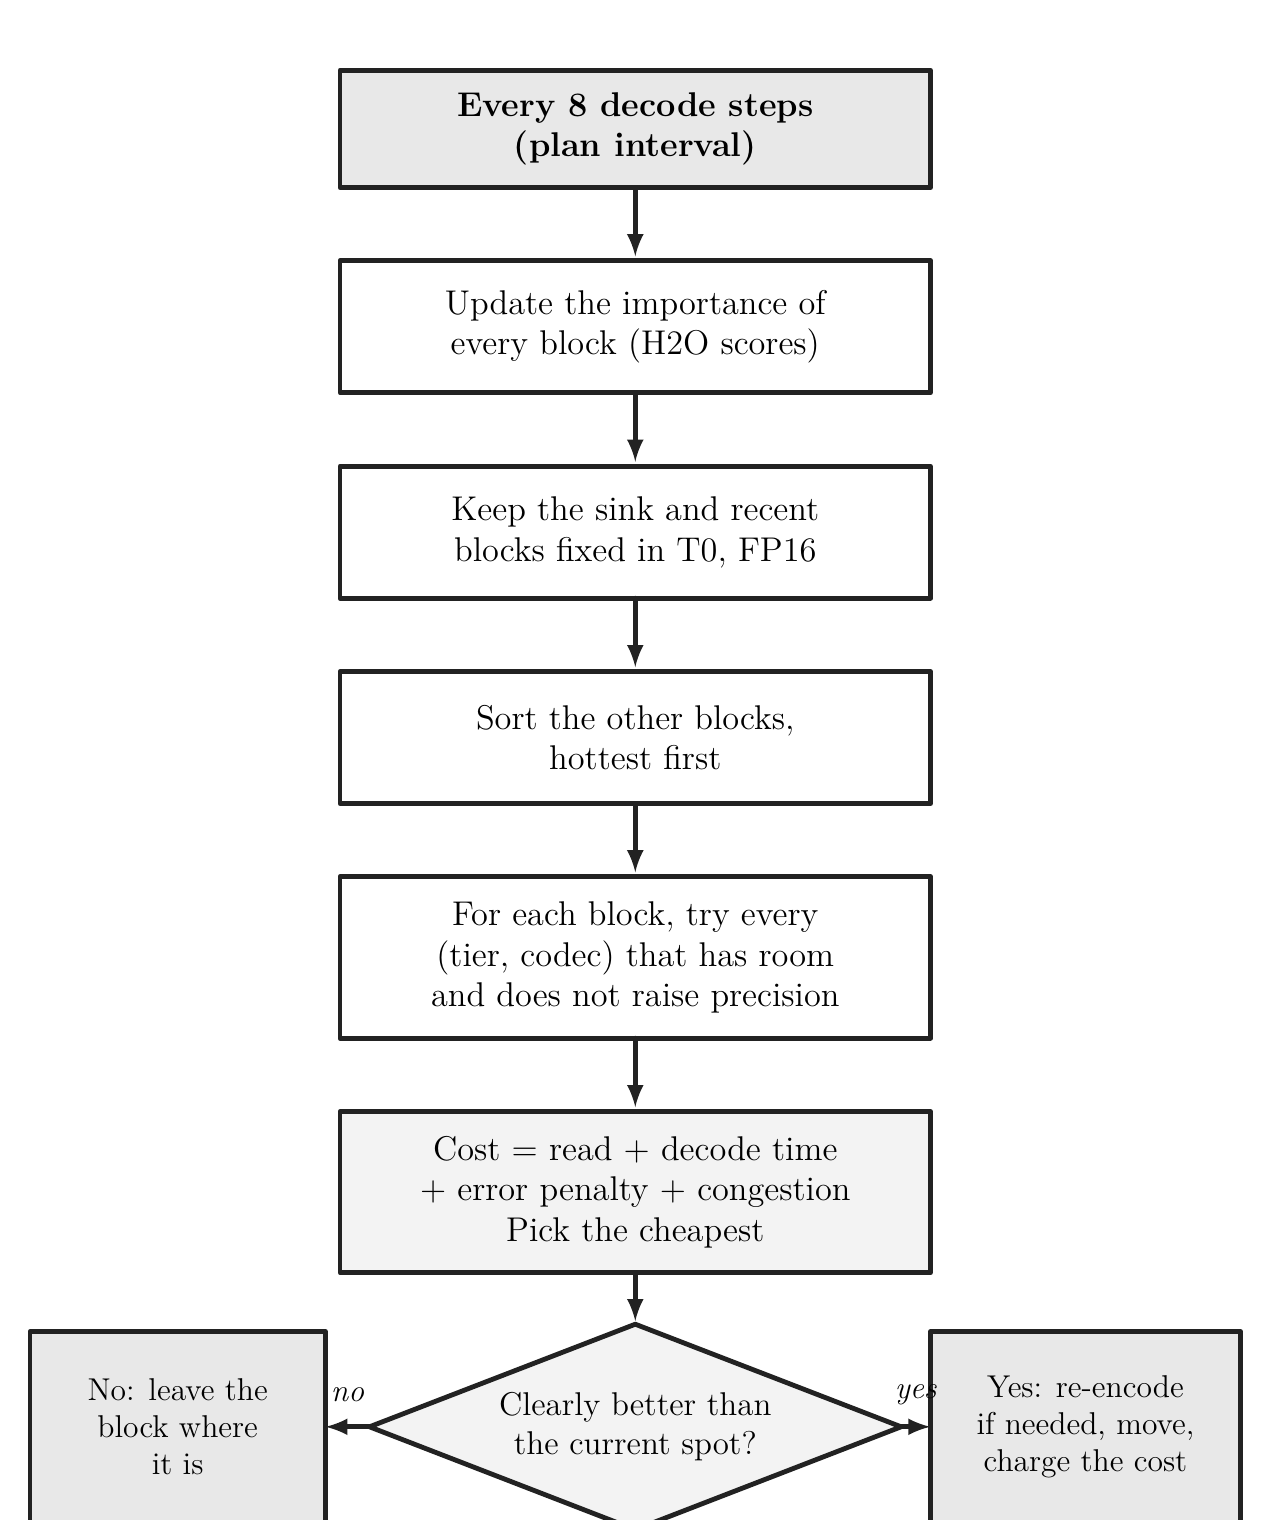
\begin{tikzpicture}[line cap=round,line join=round]
\draw[line width=1.74pt,draw={rgb,255:red,34;green,34;blue,34},fill={rgb,255:red,232;green,232;blue,232}] (1.624in,6.893in) rectangle (4.576in,7.480in);
\draw[line width=1.74pt,draw={rgb,255:red,34;green,34;blue,34},fill={rgb,255:red,255;green,255;blue,255}] (1.624in,5.867in) rectangle (4.576in,6.527in);
\draw[line width=1.74pt,draw={rgb,255:red,34;green,34;blue,34},fill={rgb,255:red,255;green,255;blue,255}] (1.624in,4.840in) rectangle (4.576in,5.500in);
\draw[line width=1.74pt,draw={rgb,255:red,34;green,34;blue,34},fill={rgb,255:red,255;green,255;blue,255}] (1.624in,3.813in) rectangle (4.576in,4.473in);
\draw[line width=1.74pt,draw={rgb,255:red,34;green,34;blue,34},fill={rgb,255:red,255;green,255;blue,255}] (1.624in,2.640in) rectangle (4.576in,3.447in);
\draw[line width=1.74pt,draw={rgb,255:red,34;green,34;blue,34},fill={rgb,255:red,243;green,243;blue,243}] (1.624in,1.467in) rectangle (4.576in,2.273in);
\draw[line width=1.74pt,draw={rgb,255:red,34;green,34;blue,34},fill={rgb,255:red,243;green,243;blue,243}] (3.100in,1.210in) -- (4.429in,0.697in) -- (3.100in,0.183in) -- (1.771in,0.697in) -- cycle;
\draw[line width=1.74pt,draw={rgb,255:red,34;green,34;blue,34},fill={rgb,255:red,232;green,232;blue,232}] (4.576in,0.220in) rectangle (6.126in,1.173in);
\draw[line width=1.74pt,draw={rgb,255:red,34;green,34;blue,34},fill={rgb,255:red,232;green,232;blue,232}] (0.074in,0.220in) rectangle (1.550in,1.173in);
\node[align=center,text={rgb,255:red,0;green,0;blue,0},font=\fontsize{12.4pt}{14.6pt}\selectfont\bfseries,inner sep=0pt] at (3.100in,7.187in) {Every 8 decode steps \\ (plan interval)};
\node[align=center,text={rgb,255:red,0;green,0;blue,0},font=\fontsize{12.4pt}{14.6pt}\selectfont,inner sep=0pt] at (3.100in,6.197in) {Update the importance of \\ every block (H2O scores)};
\node[align=center,text={rgb,255:red,0;green,0;blue,0},font=\fontsize{12.4pt}{14.6pt}\selectfont,inner sep=0pt] at (3.100in,5.170in) {Keep the sink and recent \\ blocks fixed in T0, FP16};
\node[align=center,text={rgb,255:red,0;green,0;blue,0},font=\fontsize{12.4pt}{14.6pt}\selectfont,inner sep=0pt] at (3.100in,4.143in) {Sort the other blocks, \\ hottest first};
\node[align=center,text={rgb,255:red,0;green,0;blue,0},font=\fontsize{12.4pt}{14.6pt}\selectfont,inner sep=0pt] at (3.100in,3.043in) {For each block, try every \\ (tier, codec) that has room \\ and does not raise precision};
\node[align=center,text={rgb,255:red,0;green,0;blue,0},font=\fontsize{12.4pt}{14.6pt}\selectfont,inner sep=0pt] at (3.100in,1.870in) {Cost = read + decode time \\ + error penalty + congestion \\ Pick the cheapest};
\node[align=center,text={rgb,255:red,0;green,0;blue,0},font=\fontsize{11.9pt}{14.0pt}\selectfont,inner sep=0pt] at (3.100in,0.697in) {Clearly better than \\ the current spot?};
\draw[-latex,line width=1.74pt,draw={rgb,255:red,34;green,34;blue,34}] (3.100in,6.893in) -- (3.100in,6.549in);
\draw[-latex,line width=1.74pt,draw={rgb,255:red,34;green,34;blue,34}] (3.100in,5.867in) -- (3.100in,5.522in);
\draw[-latex,line width=1.74pt,draw={rgb,255:red,34;green,34;blue,34}] (3.100in,4.840in) -- (3.100in,4.495in);
\draw[-latex,line width=1.74pt,draw={rgb,255:red,34;green,34;blue,34}] (3.100in,3.813in) -- (3.100in,3.469in);
\draw[-latex,line width=1.74pt,draw={rgb,255:red,34;green,34;blue,34}] (3.100in,2.640in) -- (3.100in,2.295in);
\draw[-latex,line width=1.74pt,draw={rgb,255:red,34;green,34;blue,34}] (3.100in,1.467in) -- (3.100in,1.225in);
\node[align=center,text={rgb,255:red,0;green,0;blue,0},font=\fontsize{11.4pt}{13.5pt}\selectfont,inner sep=0pt] at (5.351in,0.697in) {Yes: re-encode \\ if needed, move, \\ charge the cost};
\node[align=center,text={rgb,255:red,0;green,0;blue,0},font=\fontsize{11.4pt}{13.5pt}\selectfont,inner sep=0pt] at (0.812in,0.697in) {No: leave the \\ block where \\ it is};
\draw[-latex,line width=1.74pt,draw={rgb,255:red,34;green,34;blue,34}] (4.429in,0.697in) -- (4.576in,0.697in);
\node[align=center,text={rgb,255:red,0;green,0;blue,0},font=\fontsize{11.4pt}{13.5pt}\selectfont\itshape,inner sep=0pt] at (4.502in,0.858in) {yes};
\draw[-latex,line width=1.74pt,draw={rgb,255:red,34;green,34;blue,34}] (1.771in,0.697in) -- (1.550in,0.697in);
\node[align=center,text={rgb,255:red,0;green,0;blue,0},font=\fontsize{11.4pt}{13.5pt}\selectfont\itshape,inner sep=0pt] at (1.661in,0.858in) {no};
\end{tikzpicture}
}
\caption{Planner flow: candidate enumeration, cost evaluation, greedy capacity-aware selection and the hysteresis check.}
\end{figure}
\subsection{Selective attention: reading less}\label{sec:5_7}
At each decode step, protected blocks (sinks, recent window and the open block) are always read. Of the remaining sealed blocks, the engine reads only the \texttt{attn\_\allowbreak{}\allowbreak{}block\_\allowbreak{}\allowbreak{}budget} (default 24) blocks with the largest upper bound on the query–key score, computed from the resident kmin/kmax summaries:

\begin{center}\small\textit{bound(b) = Σ\_\allowbreak{}c max( q\_\allowbreak{}c · kmin\_\allowbreak{}c , q\_\allowbreak{}c · kmax\_\allowbreak{}c ) ≥ q · k   for every key k in b}\end{center}
The bound holds because each product q\_\allowbreak{}c·k\_\allowbreak{}c, for k\_\allowbreak{}c between kmin\_\allowbreak{}c and kmax\_\allowbreak{}c, is at most the larger of the two endpoint products. A block with a low bound cannot contain a key that scores highly against this query, so it is neither fetched nor decoded. The test suite checks the bound property on random data. Selected blocks are decoded and attention is computed over the union of protected and selected tokens.

This is where capacity savings and bandwidth savings combine. Because skipped blocks are never touched, they can be stored in the cheapest (slowest, smallest) tier\index{tier} and codec\index{codec} without most steps ever paying for that choice; and because tier and codec are chosen on measured heat, the blocks that are touched are the ones that the system placed where they are cheap to read.

\begin{figure}[htbp]
\centering
\adjustbox{max width=\linewidth}{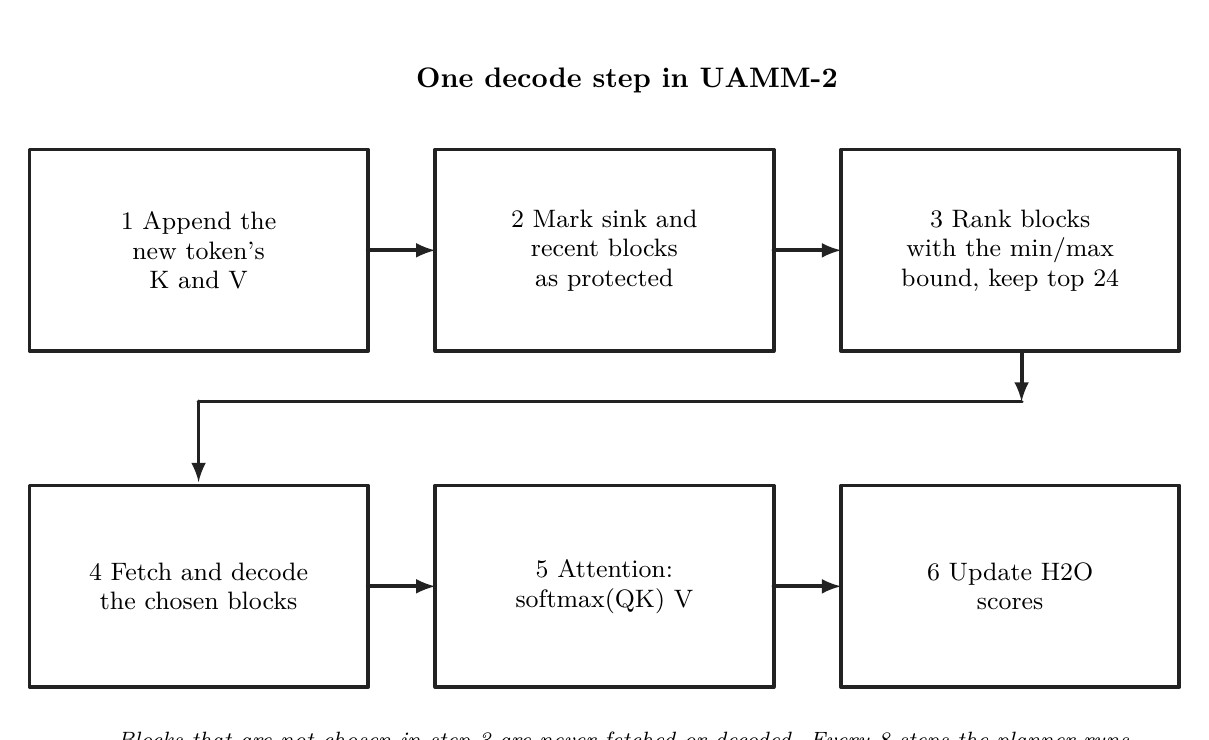
\begin{tikzpicture}[line cap=round,line join=round]
\draw[line width=1.38pt,draw={rgb,255:red,34;green,34;blue,34},fill={rgb,255:red,255;green,255;blue,255}] (0.113in,2.128in) rectangle (1.804in,3.136in);
\draw[line width=1.38pt,draw={rgb,255:red,34;green,34;blue,34},fill={rgb,255:red,255;green,255;blue,255}] (2.142in,2.128in) rectangle (3.833in,3.136in);
\draw[line width=1.38pt,draw={rgb,255:red,34;green,34;blue,34},fill={rgb,255:red,255;green,255;blue,255}] (4.171in,2.128in) rectangle (5.862in,3.136in);
\draw[line width=1.38pt,draw={rgb,255:red,34;green,34;blue,34},fill={rgb,255:red,255;green,255;blue,255}] (0.113in,0.448in) rectangle (1.804in,1.456in);
\draw[line width=1.38pt,draw={rgb,255:red,34;green,34;blue,34},fill={rgb,255:red,255;green,255;blue,255}] (2.142in,0.448in) rectangle (3.833in,1.456in);
\draw[line width=1.38pt,draw={rgb,255:red,34;green,34;blue,34},fill={rgb,255:red,255;green,255;blue,255}] (4.171in,0.448in) rectangle (5.862in,1.456in);
\draw[line width=1.38pt,draw={rgb,255:red,34;green,34;blue,34}] (5.073in,1.876in) -- (0.958in,1.876in);
\node[align=center,text={rgb,255:red,0;green,0;blue,0},font=\fontsize{9.1pt}{10.7pt}\selectfont,inner sep=0pt] at (0.958in,2.632in) {1  Append the \\ new token's \\ K and V};
\draw[-latex,line width=1.38pt,draw={rgb,255:red,34;green,34;blue,34}] (1.804in,2.632in) -- (2.142in,2.632in);
\node[align=center,text={rgb,255:red,0;green,0;blue,0},font=\fontsize{9.1pt}{10.7pt}\selectfont,inner sep=0pt] at (2.987in,2.632in) {2  Mark sink and \\ recent blocks \\ as protected};
\draw[-latex,line width=1.38pt,draw={rgb,255:red,34;green,34;blue,34}] (3.833in,2.632in) -- (4.171in,2.632in);
\node[align=center,text={rgb,255:red,0;green,0;blue,0},font=\fontsize{9.1pt}{10.7pt}\selectfont,inner sep=0pt] at (5.016in,2.632in) {3  Rank blocks \\ with the min/max \\ bound, keep top 24};
\node[align=center,text={rgb,255:red,0;green,0;blue,0},font=\fontsize{9.1pt}{10.7pt}\selectfont,inner sep=0pt] at (0.958in,0.952in) {4  Fetch and decode \\ the chosen blocks};
\draw[-latex,line width=1.38pt,draw={rgb,255:red,34;green,34;blue,34}] (1.804in,0.952in) -- (2.142in,0.952in);
\node[align=center,text={rgb,255:red,0;green,0;blue,0},font=\fontsize{9.1pt}{10.7pt}\selectfont,inner sep=0pt] at (2.987in,0.952in) {5  Attention: \\ softmax(QK) V};
\draw[-latex,line width=1.38pt,draw={rgb,255:red,34;green,34;blue,34}] (3.833in,0.952in) -- (4.171in,0.952in);
\node[align=center,text={rgb,255:red,0;green,0;blue,0},font=\fontsize{9.1pt}{10.7pt}\selectfont,inner sep=0pt] at (5.016in,0.952in) {6  Update H2O \\ scores};
\draw[-latex,line width=1.38pt,draw={rgb,255:red,34;green,34;blue,34}] (5.073in,2.128in) -- (5.073in,1.876in);
\draw[-latex,line width=1.38pt,draw={rgb,255:red,34;green,34;blue,34}] (0.958in,1.876in) -- (0.958in,1.473in);
\node[anchor=south,align=center,text={rgb,255:red,0;green,0;blue,0},font=\fontsize{10.2pt}{12.0pt}\selectfont\bfseries,inner sep=0pt] at (3.100in,3.416in) {One decode step in UAMM-2};
\node[anchor=south,align=center,text={rgb,255:red,0;green,0;blue,0},font=\fontsize{8.0pt}{9.4pt}\selectfont\itshape,inner sep=0pt] at (3.100in,0.123in) {Blocks that are not chosen in step 3 are never fetched or decoded. Every 8 steps the planner runs.};
\end{tikzpicture}
}
\caption{One decode step: bound ranking, fetch of selected blocks, attention, H2O update and (every few steps) a planning pass.}
\end{figure}
\subsection{Hardware: three verified RTL blocks}\label{sec:5_8}
Three modules were written in synthesisable Verilog-2001. Each has a bit-exact Python golden model (\texttt{uamm2/\allowbreak{}hwmodel.\allowbreak{}py}), generated test vectors and a self-checking testbench run in Verilator\index{Verilator}. They accelerate the \textit{inner loops} of the system; the utility planner\index{planner} itself remains software.

\subsubsection{Sweep scorer (\texttt{uamm\_\allowbreak{}\allowbreak{}sweep\_\allowbreak{}\allowbreak{}scorer})}\label{sec:5_8_1}
The scorer is the hardware heat classifier derived from UAMM-1\index{UAMM-1}. Block metadata is held in a small SRAM as a 25-bit word \texttt{\{protected, frequency[7:0], recency[7:0], importance[7:0]\}}. A \texttt{start} pulse latches an 8-bit memory-pressure value and launches a \textbf{sweep}: every block is read (one per cycle), passes through a 2-stage pipeline, and emerges as a result record \texttt{\{idx, score, tier, evict\}}. The score is computed without a divider:

\begin{center}\small\textit{score = ( 154·imp + 64·rec + 38·frq ) >> 8      (154 + 64 + 38 = 256)}\end{center}
The tier\index{tier} is hot if the block is protected or score ≥ 174, warm if score ≥ 89, otherwise cold. A block is flagged for eviction only if it is \textbf{not} protected, the latched pressure is at least 243, and its score is below 89. A sweep over 64 blocks has latency NBLK + 3 cycles and completes with a \texttt{done} pulse; a \texttt{start} received while busy is ignored.

\begin{figure}[htbp]
\centering
\adjustbox{max width=\linewidth}{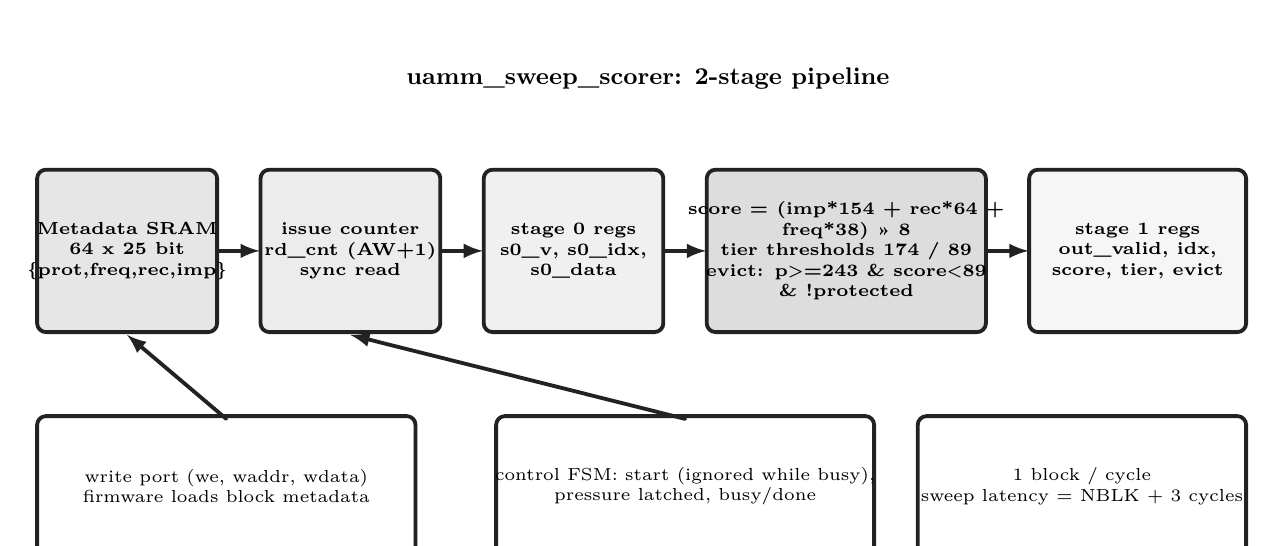
\begin{tikzpicture}[line cap=round,line join=round]
\draw[rounded corners=3.2pt,line width=1.38pt,draw={rgb,255:red,34;green,34;blue,34},fill={rgb,255:red,230;green,230;blue,230}] (0.046in,1.442in) rectangle (0.946in,2.254in);
\draw[rounded corners=3.2pt,line width=1.38pt,draw={rgb,255:red,34;green,34;blue,34},fill={rgb,255:red,236;green,236;blue,236}] (1.163in,1.442in) rectangle (2.062in,2.254in);
\draw[rounded corners=3.2pt,line width=1.38pt,draw={rgb,255:red,34;green,34;blue,34},fill={rgb,255:red,240;green,240;blue,240}] (2.279in,1.442in) rectangle (3.177in,2.254in);
\draw[rounded corners=3.2pt,line width=1.38pt,draw={rgb,255:red,34;green,34;blue,34},fill={rgb,255:red,221;green,221;blue,221}] (3.394in,1.442in) rectangle (4.790in,2.254in);
\draw[rounded corners=3.2pt,line width=1.38pt,draw={rgb,255:red,34;green,34;blue,34},fill={rgb,255:red,246;green,246;blue,246}] (5.006in,1.442in) rectangle (6.091in,2.254in);
\draw[-latex,line width=1.38pt,draw={rgb,255:red,34;green,34;blue,34}] (0.949in,1.848in) -- (1.159in,1.848in);
\draw[-latex,line width=1.38pt,draw={rgb,255:red,34;green,34;blue,34}] (2.065in,1.848in) -- (2.275in,1.848in);
\draw[-latex,line width=1.38pt,draw={rgb,255:red,34;green,34;blue,34}] (3.181in,1.848in) -- (3.391in,1.848in);
\draw[-latex,line width=1.38pt,draw={rgb,255:red,34;green,34;blue,34}] (4.793in,1.848in) -- (5.003in,1.848in);
\draw[rounded corners=3.2pt,line width=1.38pt,draw={rgb,255:red,34;green,34;blue,34},fill={rgb,255:red,255;green,255;blue,255}] (0.046in,0.322in) rectangle (1.938in,1.022in);
\draw[rounded corners=3.2pt,line width=1.38pt,draw={rgb,255:red,34;green,34;blue,34},fill={rgb,255:red,255;green,255;blue,255}] (2.341in,0.322in) rectangle (4.231in,1.022in);
\draw[rounded corners=3.2pt,line width=1.38pt,draw={rgb,255:red,34;green,34;blue,34},fill={rgb,255:red,255;green,255;blue,255}] (4.449in,0.322in) rectangle (6.091in,1.022in);
\draw[-latex,line width=1.38pt,draw={rgb,255:red,34;green,34;blue,34}] (0.992in,1.008in) -- (0.496in,1.428in);
\draw[-latex,line width=1.38pt,draw={rgb,255:red,34;green,34;blue,34}] (3.286in,1.008in) -- (1.612in,1.428in);
\node[align=center,text={rgb,255:red,0;green,0;blue,0},font=\fontsize{6.3pt}{7.4pt}\selectfont\bfseries,inner sep=0pt] at (0.496in,1.848in) {Metadata SRAM \\ 64 x 25 bit \\ \{prot,freq,rec,imp\}};
\node[align=center,text={rgb,255:red,0;green,0;blue,0},font=\fontsize{6.3pt}{7.4pt}\selectfont\bfseries,inner sep=0pt] at (1.612in,1.848in) {issue counter \\ rd\_cnt (AW+1) \\ sync read};
\node[align=center,text={rgb,255:red,0;green,0;blue,0},font=\fontsize{6.3pt}{7.4pt}\selectfont\bfseries,inner sep=0pt] at (2.728in,1.848in) {stage 0 regs \\ s0\_v, s0\_idx, \\ s0\_data};
\node[align=center,text={rgb,255:red,0;green,0;blue,0},font=\fontsize{6.3pt}{7.4pt}\selectfont\bfseries,inner sep=0pt] at (4.092in,1.848in) {score = (imp*154 + rec*64 + \\ freq*38) >> 8 \\ tier thresholds 174 / 89 \\ evict: p>=243 \& score<89 \\ \& !protected};
\node[align=center,text={rgb,255:red,0;green,0;blue,0},font=\fontsize{6.3pt}{7.4pt}\selectfont\bfseries,inner sep=0pt] at (5.549in,1.848in) {stage 1 regs \\ out\_valid, idx, \\ score, tier, evict};
\node[align=center,text={rgb,255:red,0;green,0;blue,0},font=\fontsize{6.3pt}{7.4pt}\selectfont,inner sep=0pt] at (0.992in,0.672in) {write port (we, waddr, wdata) \\ firmware loads block metadata};
\node[align=center,text={rgb,255:red,0;green,0;blue,0},font=\fontsize{6.3pt}{7.4pt}\selectfont,inner sep=0pt] at (3.286in,0.672in) {control FSM: start (ignored while busy), \\ pressure latched, busy/done};
\node[align=center,text={rgb,255:red,0;green,0;blue,0},font=\fontsize{6.3pt}{7.4pt}\selectfont,inner sep=0pt] at (5.270in,0.672in) {1 block / cycle \\ sweep latency = NBLK + 3 cycles};
\node[anchor=south,align=center,text={rgb,255:red,0;green,0;blue,0},font=\fontsize{8.7pt}{10.3pt}\selectfont\bfseries,inner sep=0pt] at (3.100in,2.653in) {uamm\_sweep\_scorer: 2-stage pipeline};
\end{tikzpicture}
}
\caption{Sweep scorer micro-architecture: metadata SRAM, weighted sum, threshold comparators, protected override and eviction logic.}
\end{figure}
\subsubsection{KV codec pipeline (\texttt{uamm\_\allowbreak{}\allowbreak{}kv\_\allowbreak{}\allowbreak{}quant4}, \texttt{uamm\_\allowbreak{}\allowbreak{}kv\_\allowbreak{}\allowbreak{}dequant4})}\label{sec:5_8_2}
The quantiser processes 16 byte-wide lanes per beat. Software or firmware supplies per-group parameters derived from the group's min and max: the zero point \texttt{zp}, a Q4.12 reciprocal \texttt{inv\_\allowbreak{}\allowbreak{}q12 = round(15·4096/\allowbreak{}range)} and a Q8.8 step \texttt{step\_\allowbreak{}\allowbreak{}q8 = round(range·256/\allowbreak{}15)}. Quantisation is q = clamp(((x − zp)·inv + 2048) >> 12, 0, 15) with x < zp clamped to zero; dequantisation is x' = min(255, zp + ((q·step + 128) >> 8)). Each module has one pipeline register. The output is packed with lane i in nibble i, matching the software packing. The intended location is on the AXI stream between memory and Ara\index{Ara}'s vector load/store unit, so that (de)quantisation\index{quantisation} happens in the load path rather than in vector instructions.

\subsubsection{Block table (\texttt{uamm\_\allowbreak{}\allowbreak{}block\_\allowbreak{}\allowbreak{}table})}\label{sec:5_8_3}
A direct-mapped translation table maps a logical block index (8 bits, 256 entries) to \texttt{\{tier[1:0], codec[1:0], phys[11:0]\}} with a separate valid bit that is cleared by reset. A lookup is a one-cycle synchronous read that returns the entry and a \texttt{hit} flag. A read in the same cycle as a write to the same address returns the \textbf{old} entry, a property fixed by design and verified by test.

\subsection{The vector kernel for the Ara vector processor}\label{sec:5_9}
Ara\index{Ara} is a RISC-V\index{RISC-V} Vector coprocessor. Attention scores for a block of 4-bit keys can be computed without first dequantising the keys into floating point. Because the key for token t at channel c is x = q·s\_\allowbreak{}c + z\_\allowbreak{}c, the dot product with a query splits into:

\begin{center}\small\textit{q · k\_\allowbreak{}t = Σ\_\allowbreak{}c ( q\_\allowbreak{}c · s\_\allowbreak{}c ) · Q[t,c]  +  Σ\_\allowbreak{}c q\_\allowbreak{}c · z\_\allowbreak{}c}\end{center}
The first term uses the integer codes Q and a query vector pre-scaled by the per-channel scales (computed once per block); the second term is a constant for the block (the \textbf{bias}). The kernel therefore folds scales and zeros into the query once, then, for each token, loads packed bytes with a vector byte load, extracts the low and high nibbles (even and odd channels), zero-extends and converts them to float, and accumulates with fused multiply–add into two pre-scaled query halves, finishing with a vector reduction. No expanded floating-point key block is ever written to memory.

A scalar version of the kernel with identical data layout runs on the host and is checked against NumPy (Section~\ref{sec:10}). The RVV version uses the standard intrinsics and compiles for \texttt{rv64gcv}. It has not been executed (Chapter~\ref{sec:12}).

\subsection{The runtime seam and the codec slot}\label{sec:5_10}
A narrow \texttt{RuntimeAdapter} interface (write token, read block, migrate block, report attention importance) separates the engine from any inference framework. \texttt{ReferenceAdapter} implements it on the NumPy engine and is exercised in the tests. \texttt{RuntimeAdapter skeleton for a compiler-based runtime} is a skeleton whose docstring lists the integration steps: map to the runtime's KV pages, obtain attention weights (fused attention kernels do not normally expose them, so a row-sum output or a side kernel is needed), perform synchronised tensor movement, and confirm that the compiler can target RVV.

The codec\index{codec} layer exposes \texttt{encode(k, v, codec, v\_\allowbreak{}\allowbreak{}group) → Payload} and \texttt{decode(Payload) → (k, v)}. The group quantiser and outlier handling of a hardware compression engine, or any other codec, can be wired in by implementing the same interface and registering a codec name.

\section{UAMM-2 code: structure and how to run it}
\section{Project Structure and Code Walkthrough}\label{sec:6}
This chapter explains how the project is organised and what each part of the code does, so that a reader can find any behaviour described in this report.

\subsection{Directory layout}\label{sec:6_1}
\begin{lstlisting}
uamm2_project/
  README.md  requirements.txt
  uamm2/                 Python reference engine
    config.py              all parameters and the assumed cost constants
    codecs.py              quantisation, packing, entropy coding, calibration
    paged_cache.py         blocks, sealing, re-encoding, dropping
    tiers.py               tier usage and the latency model
    h2o.py                 attention-based importance
    attention.py           block selection, sparse attention, dense oracle
    planner.py             utility planner and the original threshold planner
    simulator.py           decode loop, metrics, per-step trace
    workload.py            synthetic query/key/value generator
    ablation.py cli.py __main__.py     variants and command line
    hwmodel.py             bit-exact models of the RTL + test-vector writer
    ara.py                 host build of the C kernel; RISC-V compile check
    runtime.py             runtime adapter interface, reference adapter, skeleton
  hw/
    rtl/                   uamm_sweep_scorer.v  uamm_kv_codec.v  uamm_block_table.v
    tb/                    self-checking testbenches (+trace writes VCD files)
    vectors/               generated stimulus and expected outputs (hex)
    Makefile               test, lint, vectors, clean
  ara/                     kv_kernels.c / .h : scalar and RISC-V vector kernel
  tests/                   59 pytest tests
  experiments/             run_experiments.py, mutation_test.py, figure scripts, results/
  docs/                    waveform dumps, synthesis reports, captured tool output
  report/                  scripts that build this document
\end{lstlisting}
\subsection{Python engine, module by module}\label{sec:6_2}
{\fontsize{8}{9.5}\selectfont\setlength{\tabcolsep}{3pt}
\begin{longtable}{>{\raggedright\arraybackslash}p{1.08in}>{\raggedright\arraybackslash}p{1.54in}>{\raggedright\arraybackslash}p{3.34in}}
\caption{Python modules.}\\
\toprule
\textbf{File} & \textbf{Main items} & \textbf{What it does} \\\midrule\endfirsthead
\toprule \textbf{File} & \textbf{Main items} & \textbf{What it does} \\\midrule\endhead
\bottomrule\endfoot
\texttt{config.\allowbreak{}py} & \texttt{Config}, \texttt{TierSpec} & Holds geometry (64 channels, 16-token blocks), protection (4 sinks, 32 recent), planner settings (interval 8, hysteresis 0.25, residency 16, λ = 2), codec set and the assumed latency, bandwidth and decode constants. Validates inputs on creation. \\
\texttt{codecs.\allowbreak{}py} & \texttt{encode}, \texttt{decode}, \texttt{calibrate}, \texttt{pack\_\allowbreak{}\allowbreak{}bits}, \texttt{parse\_\allowbreak{}\allowbreak{}codec} & Turns a block of keys and values into a byte payload: asymmetric quantisation (keys per channel, values per token in groups of 32), bit packing, optional zlib. \texttt{calibrate} encodes a block with every codec and returns its error and size tables. Codec names: fp16, int8, kivi4, kivi2 and their \texttt{z} forms. \\
\texttt{paged\_\allowbreak{}\allowbreak{}cache.\allowbreak{}py} & \texttt{KVBlock}, \texttt{PagedKVCache} & \texttt{append\_\allowbreak{}\allowbreak{}token} fills the open block; at 16 tokens \texttt{\_\allowbreak{}\allowbreak{}seal} rounds to FP16, stores the payload, computes key min/max and calibrates. \texttt{reencode} changes codec (lossless for the entropy wrapper, lossy otherwise); \texttt{drop} removes a block. \\
\texttt{tiers.\allowbreak{}py} & \texttt{usage}, \texttt{read\_\allowbreak{}\allowbreak{}cost\_\allowbreak{}\allowbreak{}ms}, \texttt{move\_\allowbreak{}\allowbreak{}cost\_\allowbreak{}\allowbreak{}ms}, \texttt{decode\_\allowbreak{}\allowbreak{}cost\_\allowbreak{}\allowbreak{}ms} & Accounts bytes per tier and computes the modelled read, decode and migration costs. No data actually moves. \\
\texttt{h2o.\allowbreak{}py} & \texttt{H2OImportance} & \texttt{update} decays all token scores and adds the attention weight each token received; \texttt{refresh} aggregates to blocks (mean, max or sum) and normalises by the 95th percentile. \\
\texttt{attention.\allowbreak{}py} & \texttt{select\_\allowbreak{}\allowbreak{}blocks}, \texttt{sparse\_\allowbreak{}\allowbreak{}attention}, \texttt{dense\_\allowbreak{}\allowbreak{}oracle} & Ranks candidate blocks by the key-bound formula and returns the top budget; computes attention over the read blocks; the oracle computes full FP32 attention for the error metrics. \\
\texttt{planner.\allowbreak{}py} & \texttt{UtilityPlanner}, \texttt{ThresholdPlanner}, \texttt{codec\_\allowbreak{}\allowbreak{}allowed} & The utility planner enumerates allowed (tier, codec) pairs, evaluates the cost, visits blocks by heat, applies capacity and hysteresis and returns a plan. The threshold planner reproduces the original policy for comparison. \\
\texttt{simulator.\allowbreak{}py} & \texttt{Simulator.\allowbreak{}run} & For every token: generate q/k/v, append, update protection, select blocks, run sparse and dense attention, record metrics, update hit rates and importance, and every 8 steps plan and apply. Writes a per-step trace. \\
\texttt{workload.\allowbreak{}py} & \texttt{SyntheticWorkload} & Generates sinks, outlier channels, topic phases and local recency (Section~\ref{sec:7}). \\
\texttt{ablation.\allowbreak{}py}, \texttt{cli.\allowbreak{}py} & \texttt{variants}, \texttt{main} & Defines the ablation variants; commands \texttt{simulate}, \texttt{ablate}, \texttt{hwvectors}. \\
\texttt{hwmodel.\allowbreak{}py} & \texttt{scorer\_\allowbreak{}\allowbreak{}model}, \texttt{quant4\_\allowbreak{}\allowbreak{}model}, \texttt{dequant4\_\allowbreak{}\allowbreak{}model}, \texttt{write\_\allowbreak{}\allowbreak{}vectors} & Integer-exact copies of the RTL arithmetic and the generator of boundary and random vectors that the testbenches read. \\
\texttt{ara.\allowbreak{}py} & \texttt{AraKernels}, \texttt{rvv\_\allowbreak{}\allowbreak{}compile\_\allowbreak{}\allowbreak{}check} & Builds the C kernel for the host and calls it through ctypes to score packed 4-bit keys; compiles the vector path for a RISC-V target. \\
\texttt{runtime.\allowbreak{}py} & \texttt{RuntimeAdapter}, \texttt{ReferenceAdapter} & Interface to an inference runtime (write token, read block, migrate block, report attention); a working reference implementation and a skeleton for a compiler-based runtime. \\
\bottomrule
\end{longtable}}
\subsection{The planner in code}\label{sec:6_3}
The planner\index{planner} is the part of UAMM-2\index{UAMM-2} that replaces UAMM-1\index{UAMM-1}'s thresholds, so it is worth reading in full. \texttt{\_\allowbreak{}\allowbreak{}cost} is the formula from the design section: the read and decode time weighted by how likely the block is to be read, plus the quality penalty weighted by the block's heat, plus a price for using a scarce tier\index{tier}. \texttt{plan} sorts the movable blocks from hottest to coldest and, for each one, tries every allowed (tier, codec\index{codec}) pair that has room and does not raise precision. It keeps the cheapest pair, but stays where it is when the block moved recently or when the gain is smaller than the hysteresis\index{hysteresis} margin. If nothing fits, the block stays and the overflow is counted.

\par\smallskip\noindent\textbf{UAMM-2 planner: cost and plan (planner.py)}\par\nopagebreak
\begin{lstlisting}
class UtilityPlanner:
    def __init__(self, cfg: Config):
        self.cfg = cfg
        self.cands = [(t, c) for t in range(len(cfg.tiers)) for c in all_codec_names(cfg)
                      if codec_allowed(t, c)]

    @staticmethod
    def heat(b: KVBlock) -> float:
        return 0.5 * b.hit_ema + 0.5 * b.importance

    def _cost(self, b, t, c, nbytes, used, cap) -> float:
        cfg = self.cfg
        p = max(b.hit_ema, 0.01)
        fill = used[t] / max(cap[t], 1.0)
        return (p * read_cost_ms(cfg, t, c, nbytes)
                + cfg.lambda_quality * self.heat(b) * b.err_table[c]
                + cfg.capacity_price * (nbytes / cfg.tiers[t].capacity_bytes) * (1.0 + 4.0 * fill))

    def plan(self, blocks: List[KVBlock], step: int) -> Plan:
        cfg = self.cfg
        cap = [s.capacity_bytes * (1.0 - cfg.capacity_headroom) for s in cfg.tiers]
        used = _fixed_usage(cfg, blocks)
        movable = [b for b in blocks if b.sealed and not b.protected and not b.dropped]
        movable.sort(key=lambda b: -self.heat(b))
        plan: Plan = {}
        for b in movable:
            best, best_cost, cur, cur_cost = None, float("inf"), None, float("inf")
            for t, c in self.cands:
                if codec_rank(c) < b.rank:
                    continue
                nbytes = b.payload.nbytes if c == b.codec else b.size_table[c]
                if used[t] + nbytes > cap[t]:
                    continue
                cost = self._cost(b, t, c, nbytes, used, cap)
                if cost < best_cost:
                    best, best_cost = (t, c, nbytes), cost
                if (t, c) == (b.tier, b.codec):
                    cur, cur_cost = (t, c, nbytes), cost
            choice = best
            if cur is not None and best is not None:
                too_soon = (step - b.last_move_step) < cfg.min_residency_steps
                close = cur_cost <= best_cost + cfg.hysteresis_margin * max(best_cost, 1e-4)
                if too_soon or close:
                    choice = cur
            if choice is None:
                if cfg.allow_drop and b.importance < cfg.drop_importance:
                    plan[b.block_id] = (DROP, b.codec)
                else:      # nothing fits: stay put (counted as overflow by the simulator)
                    used[b.tier] += b.nbytes(cfg.head_dim)
                continue
            t, c, nbytes = choice
            used[t] += nbytes
            plan[b.block_id] = (t, c)
        return plan


class ThresholdPlanner:
\end{lstlisting}
\subsection{Hardware}\label{sec:6_4}
{\fontsize{8}{9.5}\selectfont\setlength{\tabcolsep}{3pt}
\begin{longtable}{>{\raggedright\arraybackslash}p{1.65in}>{\raggedright\arraybackslash}p{4.41in}}
\caption{Hardware files.}\\
\toprule
\textbf{File} & \textbf{What it does} \\\midrule\endfirsthead
\toprule \textbf{File} & \textbf{What it does} \\\midrule\endhead
\bottomrule\endfoot
\texttt{uamm\_\allowbreak{}\allowbreak{}sweep\_\allowbreak{}\allowbreak{}scorer.\allowbreak{}v} & Metadata SRAM (25-bit words) and a 2-stage pipeline. A \texttt{start} pulse latches the pressure value and streams all blocks through \texttt{score = (154·imp + 64·rec + 38·frq) >> 8}, the tier decision (protected override, thresholds 174 and 89) and the eviction flag (pressure ≥ 243, score < 89, not protected). \\
\texttt{uamm\_\allowbreak{}\allowbreak{}kv\_\allowbreak{}\allowbreak{}codec.\allowbreak{}v} & \texttt{uamm\_\allowbreak{}\allowbreak{}kv\_\allowbreak{}\allowbreak{}quant4}: 16 lanes of subtract, multiply by the Q4.12 reciprocal, round, clamp to 15, pack nibbles. \texttt{uamm\_\allowbreak{}\allowbreak{}kv\_\allowbreak{}\allowbreak{}dequant4}: multiply by the Q8.8 step, round, add zero point, saturate at 255. \\
\texttt{uamm\_\allowbreak{}\allowbreak{}block\_\allowbreak{}\allowbreak{}table.\allowbreak{}v} & 256-entry table of \texttt{\{tier, codec, phys\}} with valid bits and a one-cycle lookup returning \texttt{hit}. \\
\texttt{tb\_\allowbreak{}\allowbreak{}*.\allowbreak{}v} & Read the generated vectors, drive the module, compare every output and print PASS or FAIL; with \texttt{+trace} they write a VCD. \\
\texttt{Makefile} & \texttt{make test} regenerates vectors and runs the three benches in Verilator; \texttt{make lint} runs \texttt{-Wall} lint. \\
\bottomrule
\end{longtable}}
\subsection{Vector kernel}\label{sec:6_5}
\texttt{kv\_\allowbreak{}\allowbreak{}qk\_\allowbreak{}\allowbreak{}prepare} folds the per-channel scale into the query (split into even and odd channels) and returns the bias Σ q·zero. \texttt{kv\_\allowbreak{}\allowbreak{}qk\_\allowbreak{}\allowbreak{}dot\_\allowbreak{}\allowbreak{}kivi4\_\allowbreak{}\allowbreak{}scalar} loops over tokens and packed bytes with two multiply–adds per byte. \texttt{kv\_\allowbreak{}\allowbreak{}qk\_\allowbreak{}\allowbreak{}dot\_\allowbreak{}\allowbreak{}kivi4\_\allowbreak{}\allowbreak{}rvv} does the same with vector instructions (byte load, nibble extraction, widen, convert, fused multiply–add with tail-undisturbed policy, reduction). \texttt{kv\_\allowbreak{}\allowbreak{}qk\_\allowbreak{}\allowbreak{}dot\_\allowbreak{}\allowbreak{}kivi4} selects the vector path when compiled for a vector target.

\subsection{Tests}\label{sec:6_6}
{\fontsize{8}{9.5}\selectfont\setlength{\tabcolsep}{3pt}
\begin{longtable}{>{\raggedright\arraybackslash}p{1.81in}>{\raggedright\arraybackslash}p{0.54in}>{\raggedright\arraybackslash}p{3.62in}}
\caption{Test files.}\\
\toprule
\textbf{File} & \textbf{Tests} & \textbf{What is checked} \\\midrule\endfirsthead
\toprule \textbf{File} & \textbf{Tests} & \textbf{What is checked} \\\midrule\endhead
\bottomrule\endfoot
\texttt{test\_\allowbreak{}\allowbreak{}codecs.\allowbreak{}py} & 10 & Pack/unpack round trip and nibble order; FP16 exactness; error and size ordering across codecs; entropy variants lossless; per-channel keys beat per-token on outlier channels; constant input; bad inputs \\
\texttt{test\_\allowbreak{}\allowbreak{}cache\_\allowbreak{}\allowbreak{}h2o\_\allowbreak{}\allowbreak{}attention.\allowbreak{}py} & 8 & Block sealing and partial tail; ratchet and lossless entropy switch; the selection bound is a true upper bound; sparse equals dense when everything is read; heavy hitters rank higher; decay forgets \\
\texttt{test\_\allowbreak{}\allowbreak{}system.\allowbreak{}py} & 12 & Combined system fits without data loss; threshold policy must drop; combined system beats it on quality here; capacities respected; protected blocks stay hot and lossless; precision never increases; hysteresis lowers churn; drop only when enabled; adapter round trip; skeleton honesty \\
\texttt{test\_\allowbreak{}\allowbreak{}ara\_\allowbreak{}\allowbreak{}hw.\allowbreak{}py} & 6 & C kernel against NumPy; rejects other codecs; vector path compiles; golden scorer properties; codec error bounded; full RTL regression in Verilator \\
\bottomrule
\end{longtable}}
\subsection{How to run everything}\label{sec:6_7}
\begin{lstlisting}
pip install numpy pytest verilator        # g++ with C++20 needed for the RTL tests
python -m uamm2 simulate --tokens 1024     # one configuration
python -m uamm2 ablate --tokens 1536       # UAMM-1 vs UAMM-2 variants
python -m pytest -q tests                  # 56 tests, ~40 s
make -C hw test ; make -C hw lint          # RTL regression and lint
python experiments/run_experiments.py      # all studies -> experiments/results/*.json
python experiments/mutation_test.py        # RTL mutation testing
bash docs/gtkwave/view_waves.sh 3          # open a waveform with signals preloaded (1-6)
\end{lstlisting}
\section{What we tried, what we saw and what we decided}
The table at the end of this part collects the decisions. The paragraphs explain the thinking behind the ones that mattered most.

\subsection{Thresholds or a cost?}
UAMM-1\index{UAMM-1} placed a block by comparing a weighted score with two thresholds. It was easy to write and easy to put in Verilog, but a threshold knows nothing about how full a level is or what a codec\index{codec} would cost. On the synthetic trace\index{synthetic trace} it deleted 973 of 1,536 tokens once memory ran out. We then made a capacity-aware version of UAMM-1 so that the comparison would be fair, and it still had no way of making data smaller. We moved to a cost: the expected read and decode time of the block, plus a penalty for quantisation\index{quantisation} error weighted by how hot the block is, plus a price for scarce capacity. With a cost, adding a new codec or tier\index{tier} only adds a new option to choose from; with thresholds it adds more thresholds to tune. This was a decision by reasoning, backed by the E1 results.

\subsection{Block size}
We started with 16-token blocks because UAMM-1\index{UAMM-1} and PagedAttention\index{PagedAttention} use that size. We then tried 8 and 64 in the sensitivity experiment. Blocks of 8 reduced the error to 0.110 but needed 1,652 migrations, against 630 for 16 and 0.159 error. Blocks of 64 were coarse: the error rose to 0.341 and the budget\index{budget} overflowed by about 14 KB. Smaller blocks also mean more table entries and more key summaries, which an edge core has to store. We kept 16. This was decided by experiment.

\subsection{An importance score that does not saturate}
The importance value in UAMM-1\index{UAMM-1} was clamped to 1.0. After a short time the heavy-hitter tokens all sat at the limit and the controller could no longer tell which one mattered more. In UAMM-2\index{UAMM-2} we decay the token scores by 0.95 at every step so that old attention fades, and we normalise the block score by the 95th percentile of all blocks so that one extreme block cannot flatten the others. This was found by looking at the scores of a run and then confirmed in the sensitivity experiment.

\subsection{Which storage formats to offer}
We implemented FP16\index{FP16}, INT8\index{INT8}, KIVI\index{KIVI}-style 4-bit and KIVI-style 2-bit, and tried them in groups. FP16 with INT8 alone gave a size of 0.606 of FP16 and overflowed the budget\index{budget} by 104,704 B, so it cannot fit the trace. Using 2-bit for everything fitted and was small, but the error was 0.308 and the modelled fetch time 0.475 ms. INT8 with 4-bit fitted at an error of 0.122. Adding 2-bit as well gave the smallest size, 0.310 of FP16, at an error of 0.166. We left all four on, because the planner\index{planner} only uses 2-bit for blocks that are cold. This was decided by experiment.

\subsection{Entropy coding on top of quantisation}
We also tried zlib on the packed blocks, hoping that cold, low-precision data would compress further. On our synthetic data it made no difference to the measured size. We kept the code in the repository but did not use it in the headline results. We cannot say whether real activations would behave differently, so we treat this as undecided and not as a negative result. Entropy coding would also cost decode time on a core that has little of it to spare.

\subsection{Moving blocks too often}
In the first runs the planner\index{planner} moved blocks back and forth after almost every plan: 1,871 migrations. Each move costs bandwidth that the model does not see unless it is charged. We added three rules: a block must stay for a minimum of 16 tokens, a move must beat the current placement by a margin of 0.25, and the planner only runs every 8 tokens. Migrations fell to 630. We then varied the planning interval: replanning every 2 tokens gave 599 flash\index{flash} reads and 0.090 ms per token, but costs more planning work; every 64 tokens gave 3,326 flash reads and 0.272 ms because the plan was stale. An interval of 8 was a compromise. This was decided by experiment.

\subsection{How many blocks to read}
Reading every block at every step is what makes memory traffic large. We used a Quest\index{Quest}-style upper bound on the attention a block can receive for the current query, and then read only the blocks with the highest bounds. With a budget\index{budget} of 4 blocks the attention mass kept was only 0.568 and the error 1.10. With 24 blocks it was 0.945 and 0.159. With 48 blocks it was 0.986 and 0.07, but the fetch time rose to 0.278 ms. We chose 24. This was decided by experiment.

\subsection{Ideas we set aside}
\begin{itemize}
\item \textbf{Running the whole planner in hardware.} The cost function needs several multiplies and a division per block. We kept to the integer scorer (weights 154/64/38, shift by 8) and left the planner\index{planner} in software. This was decided by reasoning about area and about what an edge core can afford, not by synthesis.
\item \textbf{Per-token eviction.} Deleting single tokens would need a table entry per token. At 16 tokens per block the table is small enough for the memory we have. Chosen by reasoning.
\item \textbf{Large pages.} The 64-token block size above is the experiment that told us this was not a good idea for our budget\index{budget}.
\item \textbf{Learned policies.} A learned policy needs real traces and training data that we did not have. It is listed under future scope.
\item \textbf{Running a real model.} We had neither the memory nor the tools on our machines to run a full model on RISC-V\index{RISC-V}, so we kept a synthetic generator and said so wherever a number is quoted.
\end{itemize}
{\fontsize{9}{10.5}\selectfont\setlength{\tabcolsep}{3pt}
\begin{longtable}{>{\raggedright\arraybackslash}p{1.45in}>{\raggedright\arraybackslash}p{2.35in}>{\raggedright\arraybackslash}p{2.17in}}
\caption{Design decisions and how each one was reached.}\\
\toprule
\textbf{Decision} & \textbf{What we chose} & \textbf{How it was decided} \\\midrule\endfirsthead
\toprule \textbf{Decision} & \textbf{What we chose} & \textbf{How it was decided} \\\midrule\endhead
\bottomrule\endfoot
Placement rule & Cost-based planner & Reasoning, supported by E1 \\
Block size & 16 tokens & Experiment (E4) \\
Importance signal & Decay 0.95, 95th-percentile normalisation & Observation, then E4 \\
Storage formats & FP16, INT8, KIVI-4, KIVI-2 & Experiment (E1, E5b) \\
Entropy coding & Not used & Experiment: no gain on synthetic data \\
Stability & Residency 16, margin 0.25, interval 8 & Experiment (E4) \\
Blocks read per token & 24 & Experiment (E3) \\
Hardware scope & Integer scorer, codec, table & Reasoning \\
\bottomrule
\end{longtable}}
\section{Problems in the design}
Building the system and measuring it raised problems we had not planned for. The table below lists the design problems and what we did about each. The list after it covers what we changed in the way we check our own results.

\subsection{Problems in the design}
{\fontsize{8}{9.5}\selectfont\setlength{\tabcolsep}{3pt}
\begin{longtable}{>{\raggedright\arraybackslash}p{3.03in}>{\raggedright\arraybackslash}p{3.03in}}
\caption{Design problems and what we did about them.}\\
\toprule
\textbf{Problem} & \textbf{How we tackled it} \\\midrule\endfirsthead
\toprule \textbf{Problem} & \textbf{How we tackled it} \\\midrule\endhead
\bottomrule\endfoot
H2O scores are sums that grow without limit; UAMM-1 clamped them at 1.0, so heavy hitters saturated and could not be told apart. & Decay the token scores at every step and normalise block importance by the 95th percentile of all blocks. \\
We could not say how much error a codec would add to a given block. & Measure it: when a block is sealed, encode and decode it with every codec and store the relative error. The planner uses the measured value. \\
Keys have a few channels with very large values, so plain per-token quantisation wrecks them. & Follow KIVI: scale keys per channel and values per token. A test checks that per-channel keys give lower error on outlier data. \\
No real model or real activations were available on our machines. & Write a synthetic generator that has the properties we care about (a few heavy-hitter tokens, topic revisits, outlier channels), say so wherever a number is quoted, and compare variants with each other, not with an absolute bar. \\
Blocks moved back and forth between tiers after every plan. & Add a minimum residency, a required improvement margin and a plan interval. Migrations fell from 1,871 to 630. \\
The Verilog scorer divided by 100, which costs area and time. & Choose integer weights 154/64/38 that sum to 256 and shift right by 8. The codec likewise multiplies by a precomputed reciprocal. \\
The first testbench had three vectors and passed everything. & Write 17 sweeps with the threshold edge cases, 400 codec vectors, 6,000 random table operations and a mutation test. The mutation test found a quantiser clamp that no vector exercised; we added vectors until it was caught. \\
We had no Ara processor or simulator to run the vector kernel on. & Run the scalar path on the host against NumPy, compile the vector path for rv64gcv and inspect the instructions, and state clearly that it was never executed. \\
\bottomrule
\end{longtable}}
\subsection{What we do now}
\begin{itemize}
\item \textbf{Make the baseline fair before claiming a win.} The most important error was comparing against a weak baseline\index{baseline}. We asked what the simplest competent alternative would be, built it (a single 4-bit codec\index{codec} with no cost model), and let it into every table. The result changed the conclusion: the planner\index{planner} is not the reason the data fits; the codecs are.
\item \textbf{Report what is charged and what is not.} Any memory that is used but not counted flatters the result. We measured the key summaries, reported them, and ran the experiment with them charged.
\item \textbf{Separate the measurement from the model.} Latency, bandwidth and decode costs are assumptions, the workload is synthetic, no language model was run and nothing ran on Ara\index{Ara}. Each statement now says which of these it depends on.
\item \textbf{State the budget dependence.} The gain over UAMM-1\index{UAMM-1} comes from a budget\index{budget} 2.3× smaller than the data. At 3× the budget FP16\index{FP16} fits and wins. We now show the sweep next to the headline.
\item \textbf{Re-derive each number from the result files.} The text was checked against the JSON files in the repository. Every number we changed in the text is one that could be traced to an experiment.
\item \textbf{Label design ideas as design ideas.} Things that are proposed but not built are labelled as such in the chapter title and in a status note.
\item \textbf{Cite or remove.} A claim with no source was removed; a named system was cited.
\end{itemize}
\subsection{What our results show}
On a synthetic workload with assumed memory costs, a joint (tier\index{tier}, codec\index{codec}) choice lets a 168 KB budget\index{budget} hold 1,536 tokens that FP16\index{FP16} cannot, without deleting any token, where the original UAMM-1\index{UAMM-1} threshold policy deleted 63 \% of them. A simple all-4-bit baseline\index{baseline} does the same and is faster in the model. The planner\index{planner}'s measured benefits are lower output error at equal memory, lower memory with the 2-bit codec, and feasibility in tighter budgets, at the price of a higher modelled fetch time than that baseline. We claim nothing about speed on real hardware, about real language models, or about the vector processor, which only compiled the kernel.

\chapter{Simulation Results and What We Obtained}
This chapter reports what the simulations and the hardware checks showed and what we can conclude from them. It starts with what we assumed, because every number below depends on those assumptions, and ends with what we think is new in this work.

\section{What we assumed}
{\fontsize{8}{9.5}\selectfont\setlength{\tabcolsep}{3pt}
\begin{longtable}{>{\raggedright\arraybackslash}p{1.08in}>{\raggedright\arraybackslash}p{2.71in}>{\raggedright\arraybackslash}p{2.17in}}
\caption{What the results rest on.}\\
\toprule
\textbf{Assumption} & \textbf{What we used} & \textbf{Effect on the conclusions} \\\midrule\endfirsthead
\toprule \textbf{Assumption} & \textbf{What we used} & \textbf{Effect on the conclusions} \\\midrule\endhead
\bottomrule\endfoot
Workload & A synthetic stream of queries, keys and values for one head of 64 channels, with heavy-hitter tokens, topic revisits and outlier channels. No language model, no tokenizer. & Errors are relative to a dense FP32 reference on this stream. Compare variants with each other, not with a fixed bar. \\
Memory costs & Four tiers of 24, 48, 32 and 64 KB with assumed latencies and bandwidths (SRAM, two DRAM tiers, flash). Decode costs per byte assumed for each codec. & Fetch time is a model output. Changing the constants can change which variant is fastest. \\
Budget & 168 KB in total for 1,536 tokens; FP16 would need 393 KB. & The advantage over UAMM-1 exists because the budget is tight. At three times the budget FP16 simply fits. \\
Key summaries & The per-block min/max key vectors (24,576 B) are not charged in the main runs. & Charging them changes which variants fit (see the key-summary experiment). \\
Hardware & Verilator simulation against Python models. No place and route, no timing, no power. & The RTL results show functional correctness, not area or speed. \\
Vector processor & The kernel was compiled for RISC-V vector but never run on Ara or a simulator. & No speed-up from the kernel is claimed. \\
\bottomrule
\end{longtable}}
\section{Experimental Methodology}\label{sec:7}
This chapter states precisely what was simulated, what was real, how quality was measured and which constants were assumed. The goal is that a reader can judge exactly what each number in the results chapter means.

\subsection{What is real and what is modelled}\label{sec:7_1}
{\fontsize{8}{9.5}\selectfont\setlength{\tabcolsep}{3pt}
\begin{longtable}{>{\raggedright\arraybackslash}p{2.20in}>{\raggedright\arraybackslash}p{3.86in}}
\caption{Status of each element of the evaluation.}\\
\toprule
\textbf{Component} & \textbf{Status in the experiments} \\\midrule\endfirsthead
\toprule \textbf{Component} & \textbf{Status in the experiments} \\\midrule\endhead
\bottomrule\endfoot
KV tensors, codecs, packing, entropy coding & \textbf{Real computation.} Blocks are actually quantised, bit-packed, optionally zlib-compressed, decoded and used for attention. \\
Attention output and quality metrics & \textbf{Real computation} on decoded tensors, compared with a dense FP32 attention oracle over all tokens at the same step. \\
Block selection (min/max bound), importance scores, planner decisions & \textbf{Real computation} (the same code that would run on a device). \\
Q, K, V stream & \textbf{Synthetic}: produced by a parametrised trace generator, described in 6.2, not by a neural network. \\
Tier latencies, bandwidths, decode costs & \textbf{Modelled constants} (6.4). The reported latency is a model output, not a measurement. \\
RTL behaviour & \textbf{Real simulation} with Verilator, compared bit-exactly with Python golden models. \\
RVV kernel & Scalar variant executed on the host; RVV variant compiled to RISC-V vector instructions but not executed. \\
\bottomrule
\end{longtable}}
\subsection{The synthetic trace generator}\label{sec:7_2}
An LLM was not run for the experiments in this report. Instead a trace generator produces, for each decode step, a query vector and a key and value vector with the structural properties that KV-cache managers are designed around. The generator has 64 channels (\texttt{head\_\allowbreak{}\allowbreak{}dim}) and exposes these features:

\begin{itemize}
\item \textbf{Attention sinks.} The first four tokens, and 3 \% of later tokens at random, receive an extra component along a fixed “heavy” direction; the query also has a component along it. These tokens attract disproportionate attention, as heavy hitters and sinks do in real models.
\item \textbf{Outlier key channels.} One in sixteen channels of the keys is scaled by 6× (4 of 64 channels). This is the structure that motivates per-channel key quantisation\index{quantisation}.
\item \textbf{Topic phases.} Four unit topic directions are defined. Keys in each phase of 96 tokens carry that phase's topic. The query's topic follows the phase but periodically (every third phase) returns to an older topic, so that previously cold blocks become hot again and must be promoted.
\item \textbf{Local recency.} Part of the query is the direction of one of the 12 most recent keys, producing local attention.
\item \textbf{Sharpness.} The query is scaled by a factor of 4, which controls how peaked the softmax is; value vectors are independent Gaussian noise.
\end{itemize}
Because the generator is designed rather than learned, its absolute numbers must not be read as what a particular LLM would give. In particular, values that are independent noise average to a small-norm vector, which inflates the \textit{relative} L2 error of the output; the comparison of variants against each other on the same stream is the meaningful quantity. Section~\ref{sec:8} includes a measurement of how concentrated the attention on this generator is, so that the reader can compare it with concentration reported for real models.

\subsection{Metrics}\label{sec:7_3}
{\fontsize{8}{9.5}\selectfont\setlength{\tabcolsep}{3pt}
\begin{longtable}{>{\raggedright\arraybackslash}p{1.36in}>{\raggedright\arraybackslash}p{2.89in}>{\raggedright\arraybackslash}p{1.72in}}
\caption{Metrics reported in the experiments.}\\
\toprule
\textbf{Metric} & \textbf{Definition} & \textbf{Why} \\\midrule\endfirsthead
\toprule \textbf{Metric} & \textbf{Definition} & \textbf{Why} \\\midrule\endhead
\bottomrule\endfoot
\texttt{resident\_\allowbreak{}\allowbreak{}vs\_\allowbreak{}\allowbreak{}fp16} & Total bytes held across tiers divided by the FP16 size of all tokens & Memory saving (lower is better) \\
\texttt{dropped\_\allowbreak{}\allowbreak{}tokens} & Tokens permanently removed & Irreversible information loss \\
\texttt{attn\_\allowbreak{}\allowbreak{}rel\_\allowbreak{}\allowbreak{}l2} & \ensuremath{\Vert}o\_\allowbreak{}sys − o\_\allowbreak{}dense\ensuremath{\Vert} / \ensuremath{\Vert}o\_\allowbreak{}dense\ensuremath{\Vert} for the attention output at each step after a warm-up of 64 steps (mean and 95th percentile) & Output fidelity vs a dense FP32 oracle over the same (FP16-rounded) data \\
\texttt{attn\_\allowbreak{}\allowbreak{}mass\_\allowbreak{}\allowbreak{}recall} & Fraction of the oracle's attention probability that falls on the tokens the system read & How much of what attention wants was available \\
\texttt{sim\_\allowbreak{}\allowbreak{}fetch\_\allowbreak{}\allowbreak{}ms\_\allowbreak{}\allowbreak{}per\_\allowbreak{}\allowbreak{}token} & Modelled time to fetch and decode all blocks read in a step (mean) & Latency of reading the KV cache under the assumed constants \\
\texttt{flash\_\allowbreak{}\allowbreak{}block\_\allowbreak{}\allowbreak{}reads} & Count of block reads served from flash & Proxy for slow-tier traffic \\
\texttt{migrations}, \texttt{reencodes} & Cumulative counts of tier moves and codec changes & Churn (energy and bandwidth cost of management) \\
\texttt{overflow\_\allowbreak{}\allowbreak{}total} & Sum over tiers of the maximum bytes by which a tier budget was exceeded & Feasibility: non-zero means the data did not fit \\
\bottomrule
\end{longtable}}
\textbf{Interpretation guard.} The attention-mass recall\index{recall} depends only on which blocks are read and not on their precision, so it is identical for all UAMM-2\index{UAMM-2} variants that use the same selection logic; the codec\index{codec} choice shows up in the relative L2 error. A non-zero error floor remains even with FP16\index{FP16} everywhere, because block-sparse attention omits some tokens; the FP16-only variant (error 0.092 at 1,536 tokens) measures that floor.

\textbf{Accounting rule.} \texttt{resident\_\allowbreak{}\allowbreak{}vs\_\allowbreak{}\allowbreak{}fp16} and the tier\index{tier} budgets count the bytes of each block's encoded payload, including its scales and zero points. They do \textbf{not} count the small per-block summaries that the engine keeps resident for selection (key minimum and maximum, 64 values each) or the scheduling state. Stored in FP16\index{FP16}, the key summaries would add about 256 bytes per block, i.e. about 25 KB for the 96 blocks of a 1,536-token run, which is roughly 6 \% of the FP16 cache size and 15 \% of the 168 KB budget\index{budget}. The results below should be read with that omission in mind; Chapter~\ref{sec:12} lists it among the open items.

\subsection{Assumed cost constants}\label{sec:7_4}
The following constants are placeholders for an edge SoC and are not measurements. They define the latency model used by the planner\index{planner} and the simulator. Conclusions about \textit{ratios} between variants depend on them; they should be replaced by values measured on the target before any absolute claim is made.

{\fontsize{8}{9.5}\selectfont\setlength{\tabcolsep}{3pt}
\begin{longtable}{>{\raggedright\arraybackslash}p{2.17in}>{\raggedright\arraybackslash}p{1.99in}>{\raggedright\arraybackslash}p{1.81in}}
\caption{Default configuration of the experiments.}\\
\toprule
\textbf{Constant} & \textbf{Value} & \textbf{Meaning} \\\midrule\endfirsthead
\toprule \textbf{Constant} & \textbf{Value} & \textbf{Meaning} \\\midrule\endhead
\bottomrule\endfoot
T0 latency / bandwidth & 0.5 µs / 100 GB/s & Near-compute SRAM or vector register file \\
T1, T2 latency / bandwidth & 2 µs / 12.8 GB/s & LPDDR-class DRAM \\
T3 latency / bandwidth & 100 µs / 1 GB/s & Flash \\
Decode cost, fp16 / int8 / kivi4 / kivi2 & 0 / 0.05 / 0.12 / 0.20 ns per byte & Software dequantisation cost model \\
zlib decode cost & 1.0 ns per byte & Additional cost for the \texttt{z} variants \\
Tier capacities T0..T3 & 24, 48, 32, 64 KB (total 168 KB) & FP16 KV for 1,536 tokens is 393 KB \\
Block size, v\_\allowbreak{}group, sink, recent window & 16 tokens, 32 channels, 4 tokens, 32 tokens & Geometry and protection \\
Attention block budget & 24 blocks per step & Non-protected blocks fetched \\
Planner: plan interval, hysteresis, residency, λ, κ, headroom & 8 steps, 0.25, 16 steps, 2.0, 0.05, 3 \% & See Section~\ref{sec:5} \\
H2O decay, aggregation, hit\_\allowbreak{}ema & 0.95, mean, 0.9 & Importance signal \\
\bottomrule
\end{longtable}}
λ was chosen on seeds 7–9 during development; all reported experiments use other seeds (11–15), so the default configuration is evaluated on data it was not tuned on.

\subsection{Experimental design}\label{sec:7_5}
{\fontsize{8}{9.5}\selectfont\setlength{\tabcolsep}{3pt}
\begin{longtable}{>{\raggedright\arraybackslash}p{0.35in}>{\raggedright\arraybackslash}p{1.75in}>{\raggedright\arraybackslash}p{2.28in}>{\raggedright\arraybackslash}p{0.79in}>{\raggedright\arraybackslash}p{0.61in}}
\caption{Experiments performed.}\\
\toprule
\textbf{ID} & \textbf{Question} & \textbf{Variable} & \textbf{Seeds} & \textbf{Tokens} \\\midrule\endfirsthead
\toprule \textbf{ID} & \textbf{Question} & \textbf{Variable} & \textbf{Seeds} & \textbf{Tokens} \\\midrule\endhead
\bottomrule\endfoot
E1 & Does each ingredient matter? (ablation) & Policy and codec set: UAMM-1 threshold; planner with FP16 only; INT8+KIVI-4; all codecs & 5 & 1,536 \\
E2 & How does the system scale with context? & Context 512–3,072 at a fixed budget & 3 & 512–3,072 \\
E3 & How many blocks must be read? & Attention block budget 4–48 & 3 & 1,536 \\
E4 & How sensitive are the planner and importance knobs? & λ, hysteresis margin, residency, plan interval, decay, aggregation, block size & 3 & 1,536 \\
E5 & How does memory budget change the picture? & Tier budgets ×0.5 to ×3.0; and codec sets with and without entropy coding & 3 & 1,536 \\
E7 & How good are the codecs, and does the key axis matter? & Codec and outlier presence; per-channel vs per-token keys & 200 random blocks per cell & — \\
\bottomrule
\end{longtable}}
Values are reported as mean ± standard deviation across seeds. With three seeds the standard deviation is itself a rough estimate; differences smaller than about one standard deviation should not be treated as significant. The experiment code is in \texttt{experiments/\allowbreak{}run\_\allowbreak{}\allowbreak{}experiments.\allowbreak{}py}, listed in the appendices, and all raw numbers are tabulated in Appendix \ref{app:rawtables}.

\section{UAMM-1 and UAMM-2 compared}
Both systems were run on the same synthetic trace\index{synthetic trace} of 1,536 tokens with the same total memory budget\index{budget} of 168 KB. FP16\index{FP16} storage of that cache would need 393 KB, so the budget is 2.3 times too small and something has to give. The table below lists the outcome; we also include the simple baseline\index{baseline} of storing every block in 4-bit, because it is the fair question to ask of any planner\index{planner}.

{\fontsize{8}{9.5}\selectfont\setlength{\tabcolsep}{3pt}
\begin{longtable}{>{\raggedright\arraybackslash}p{1.89in}>{\raggedright\arraybackslash}p{0.74in}>{\raggedright\arraybackslash}p{0.74in}>{\raggedright\arraybackslash}p{0.74in}>{\raggedright\arraybackslash}p{0.74in}>{\raggedright\arraybackslash}p{0.82in}}
\caption{UAMM-1 against UAMM-2 and a one-codec baseline (1,536 tokens, 168 KB, mean ± std over 5 seeds).}\\
\toprule
\textbf{System} & \textbf{Tokens deleted} & \textbf{Resident / FP16} & \textbf{Attention mass kept} & \textbf{Output error} & \textbf{Fetch ms / token (model)} \\\midrule\endfirsthead
\toprule \textbf{System} & \textbf{Tokens deleted} & \textbf{Resident / FP16} & \textbf{Attention mass kept} & \textbf{Output error} & \textbf{Fetch ms / token (model)} \\\midrule\endhead
\bottomrule\endfoot
UAMM-1 (threshold policy, FP16) & 973 ± 16 & 0.367 ± 0.010 & 0.758 ± 0.016 & 0.479 ± 0.035 & 0.923 ± 0.026 \\
No planner, every block 4-bit & 0 ± 0 & 0.364 ± 0.000 & 0.939 ± 0.012 & 0.152 ± 0.015 & 0.068 ± 0.003 \\
UAMM-2, INT8 + 4-bit codecs & 0 ± 0 & 0.371 ± 0.003 & 0.939 ± 0.012 & 0.122 ± 0.014 & 0.116 ± 0.002 \\
UAMM-2, INT8 + 4-bit + 2-bit codecs & 0 ± 0 & 0.310 ± 0.001 & 0.939 ± 0.012 & 0.166 ± 0.020 & 0.112 ± 0.002 \\
\bottomrule
\end{longtable}}
\begin{sidewaysfigure}[p]
\centering
\adjustbox{max width=\linewidth,max height=0.8\textwidth}{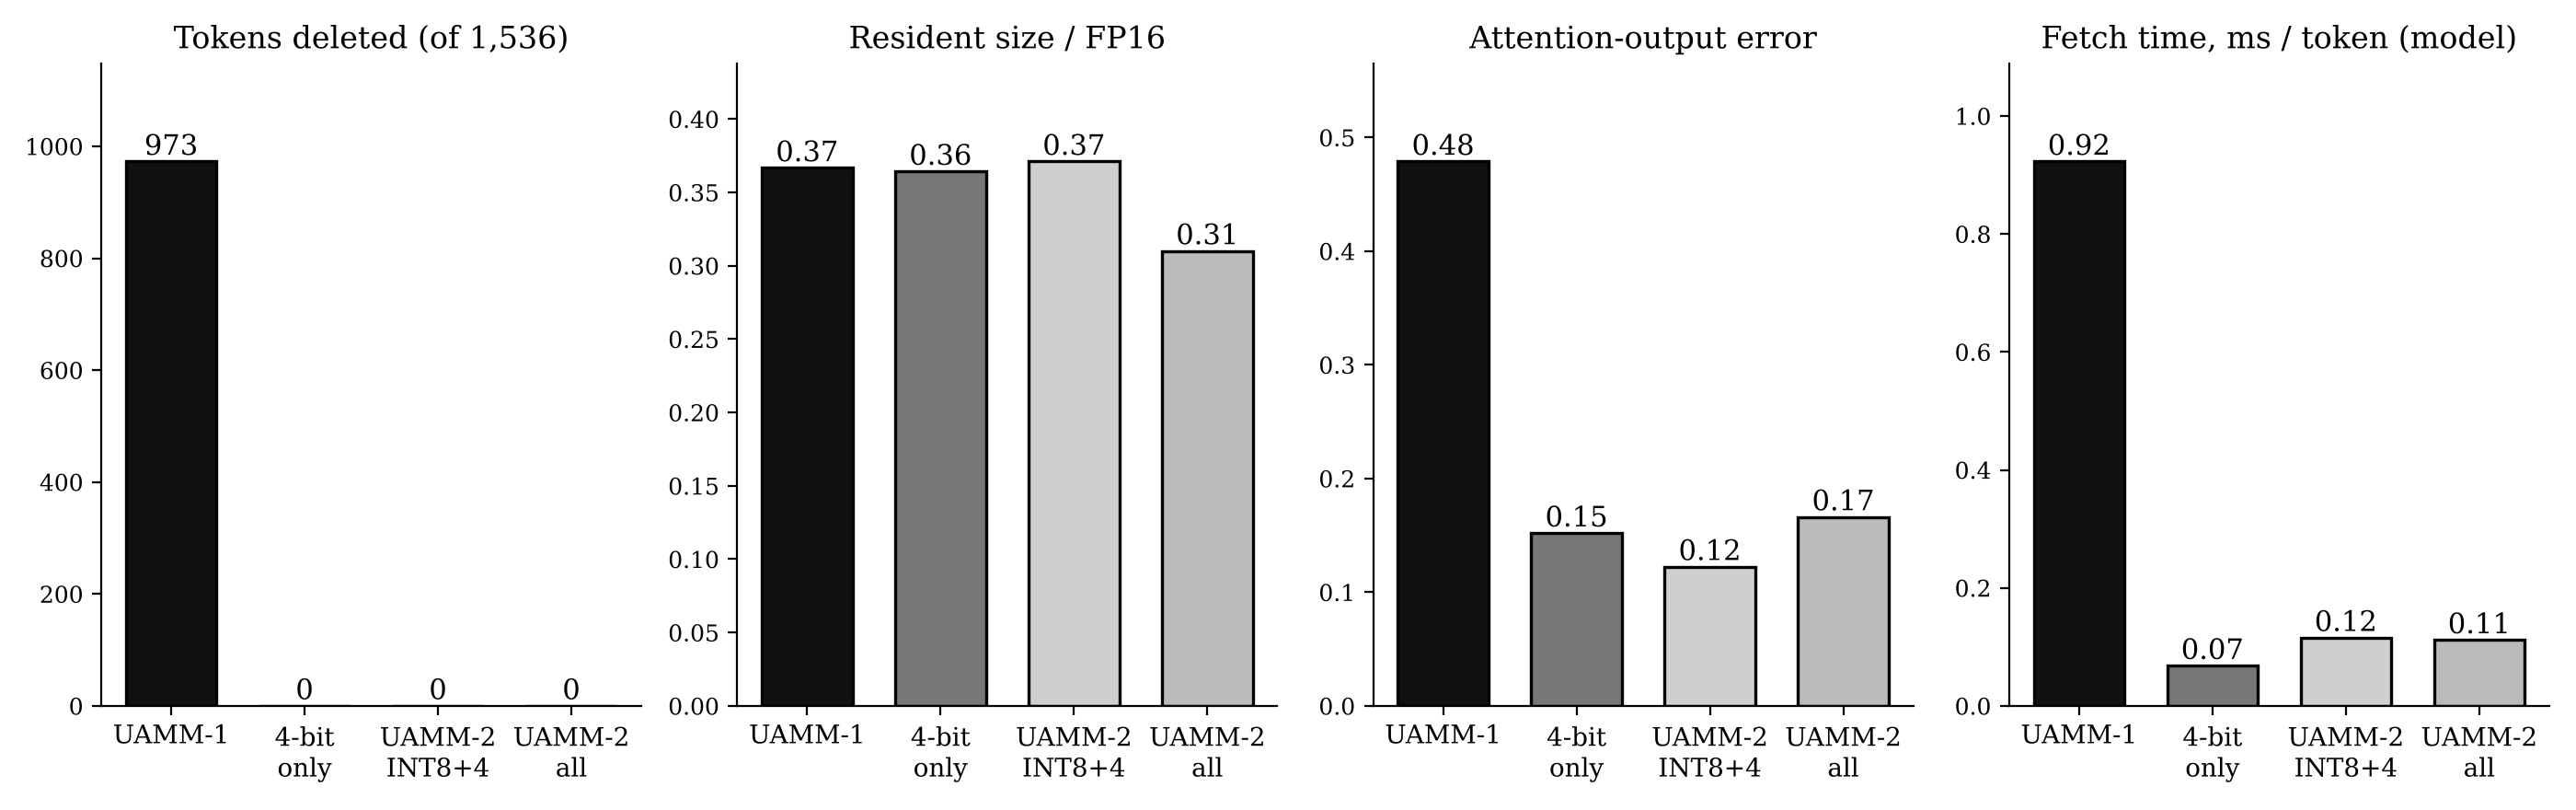
\includegraphics[width=9.30in,height=5.20in,keepaspectratio]{figs/f24_v1_v2_compare.png}}
\caption{UAMM-1 against UAMM-2 on the same trace and budget. Labels: 4-bit only = every block in 4-bit with no planner; INT8+4 = UAMM-2 with INT8 and 4-bit codecs; all = UAMM-2 with every codec.}
\end{sidewaysfigure}
\clearpage
\begin{itemize}
\item \textbf{What clearly improved.} UAMM-1\index{UAMM-1} had to delete 973 of 1,536 tokens to fit and kept 76 \% of the attention mass. UAMM-2\index{UAMM-2} keeps every token and 94 \% of the attention mass, and its output error is about a quarter to a third of UAMM-1's.
\item \textbf{What did not.} UAMM-2\index{UAMM-2} is not faster than the all-4-bit baseline\index{baseline} in our model (0.11 against 0.07 ms per token), and that baseline also keeps every token. The error of the baseline is higher (0.152 against 0.122 for UAMM-2 at the same size).
\item \textbf{So what does the planner add?} Control. It spends precision where attention actually goes, so at the same size it has lower error; with the 2-bit codec\index{codec} it reaches a smaller size; and in tighter budgets it still fits when the single-codec baseline\index{baseline} does not (Chapter~5).
\end{itemize}
\section{Simulation Results}\label{sec:8}
All numbers in this chapter come from \texttt{experiments/\allowbreak{}run\_\allowbreak{}\allowbreak{}experiments.\allowbreak{}py} (raw data in \texttt{experiments/\allowbreak{}results/\allowbreak{}*.\allowbreak{}json}) under the configuration of Section~\ref{sec:7}. Latency figures are model outputs under the assumed constants. Errors are measured against a dense FP32 oracle on the synthetic trace\index{synthetic trace}. Where we interpret a result, we say so.

\subsection{Ablation: what each ingredient contributes (E1)}\label{sec:8_1}
{\fontsize{6.5}{8.0}\selectfont\setlength{\tabcolsep}{3pt}
\begin{longtable}{>{\raggedright\arraybackslash}p{1.15in}>{\raggedright\arraybackslash}p{0.54in}>{\raggedright\arraybackslash}p{0.61in}>{\raggedright\arraybackslash}p{0.50in}>{\raggedright\arraybackslash}p{0.54in}>{\raggedright\arraybackslash}p{0.50in}>{\raggedright\arraybackslash}p{0.57in}>{\raggedright\arraybackslash}p{0.50in}>{\raggedright\arraybackslash}p{0.50in}}
\caption{Ablation and baselines at 1,536 tokens (mean ± std over 5 seeds). The first column of sizes does not count the key min/max summaries; the second does.}\\
\toprule
\textbf{Variant} & \textbf{Resident / FP16} & \textbf{Resident + summaries} & \textbf{Dropped tokens} & \textbf{Rel. L2 error} & \textbf{Mass recall} & \textbf{Fetch ms / token (model)} & \textbf{Flash reads} & \textbf{Overflow (B)} \\\midrule\endfirsthead
\toprule \textbf{Variant} & \textbf{Resident / FP16} & \textbf{Resident + summaries} & \textbf{Dropped tokens} & \textbf{Rel. L2 error} & \textbf{Mass recall} & \textbf{Fetch ms / token (model)} & \textbf{Flash reads} & \textbf{Overflow (B)} \\\midrule\endhead
\bottomrule\endfoot
UAMM-1 threshold policy, FP16 & 0.367 ± 0.0102 & 0.412 ± 0.0115 & 973 ± 16 & 0.479 ± 0.0346 & 0.758 ± 0.0164 & 0.923 ± 0.0259 & 12613 ± 374 & 0 ± 0 \\
UAMM-1 made capacity-aware, FP16 & 0.406 ± 0 & 0.457 ± 0 & 912 ± 0 & 0.406 ± 0.0305 & 0.792 ± 0.0116 & 0.618 ± 0.00894 & 8205 ± 129 & 0 ± 0 \\
No planner: every block 4-bit & 0.364 ± 0 & 0.489 ± 5.55e-17 & 0 ± 0 & 0.152 ± 0.015 & 0.939 ± 0.0117 & 0.0681 ± 0.00253 & 270 ± 37 & 0 ± 0 \\
No planner: every block 2-bit & 0.243 ± 0 & 0.368 ± 0 & 0 ± 0 & 0.572 ± 0.0187 & 0.939 ± 0.0117 & 0.0493 ± 4e-06 & 0 ± 0 & 0 ± 0 \\
Planner, FP16 only & 1 ± 0 & 1.12 ± 0 & 0 ± 0 & 0.0921 ± 0.0191 & 0.939 ± 0.0117 & 1.04 ± 0.006 & 14364 ± 86 & 258048 ± 1832 \\
Planner, INT8 + KIVI-4 & 0.371 ± 0.00265 & 0.496 ± 0.00265 & 0 ± 0 & 0.122 ± 0.0137 & 0.939 ± 0.0117 & 0.116 ± 0.00216 & 970 ± 32 & 0 ± 0 \\
Planner, INT8 + KIVI-4 + KIVI-2 & 0.31 ± 0.00133 & 0.435 ± 0.00133 & 0 ± 0 & 0.166 ± 0.0203 & 0.939 ± 0.0117 & 0.112 ± 0.00203 & 915 ± 30 & 0 ± 0 \\
\bottomrule
\end{longtable}}
\textbf{Reading the table.}

\begin{itemize}
\item \textbf{UAMM-1 fits by deleting.} With only FP16\index{FP16} blocks and a 168 KB budget\index{budget} the threshold policy must remove on average 973 of 1,536 tokens (63 \%). Attention-mass recall\index{recall} falls to 0.758 and the output error reaches 0.479; the reads that remain are frequently from flash\index{flash} (about 12,600 flash block reads).
\item \textbf{A fairer UAMM-1 still deletes.} The threshold rule sends a block to the tier\index{tier} its score selects or to a slower one, so it can place data in flash\index{flash} while faster tiers have room. Letting the best-scoring blocks take the fastest tier with room (the capacity-aware variant) lowers modelled fetch time from 0.923 to 0.618 ms and error from 0.479 to 0.406, but it still drops 912 tokens, because FP16\index{FP16} alone cannot hold 393 KB in 168 KB.
\item \textbf{The planner alone cannot create space.} With FP16\index{FP16} only, the planner\index{planner} drops nothing but cannot fit: 258 KB of overflow, i.e. the data exceeds the stated budget\index{budget} by that much. The lower error (0.092) is the floor due to block-sparse selection with exact data. This variant shows that placement alone is insufficient: without a codec\index{codec}, a budget below the data size is infeasible without deletion.
\item \textbf{Codecs make the budget feasible.} Adding INT8\index{INT8} and 4-bit codecs reduces residency\index{residency} to 0.371 of FP16\index{FP16}, with no overflow and no drops. Error rises to 0.122 (vs the 0.092 floor): the price of quantisation\index{quantisation}.
\item \textbf{A single codec for everything is a strong baseline.} Storing every unprotected block in 4-bit, with no cost model, also fits the budget\index{budget} (0.364 resident), keeps every token, and reaches error 0.152 and 0.068 ms. Against it the planner\index{planner} with INT8\index{INT8} + KIVI\index{KIVI}-4 has lower error (0.122 versus 0.152) at almost the same memory (0.371), but a higher modelled fetch time (0.116 versus 0.068 ms), because it spends DRAM on higher-precision blocks and pushes other blocks to flash\index{flash}. Section~\ref{sec:8_1_1} shows that these are different points on one trade-off curve.
\item \textbf{The 2-bit codec is enabled by default and used heavily.} Enabling 2-bit lowers residency\index{residency} from 0.371 to 0.310 (a further 16 \% saving) at an error of 0.166, i.e. 36 \% more than INT8\index{INT8} + KIVI\index{KIVI}-4. It is not a rarely used option: in the final state about 49 \% of all blocks are 2-bit, 45 \% are 4-bit and 6 \% are FP16\index{FP16} or INT8. Storing everything at 2-bit reaches 0.243 resident but error 0.572.
\item \textbf{Latency model.} Modelled fetch time per token falls from 0.92 ms (UAMM-1\index{UAMM-1}) to 0.116 ms (INT8\index{INT8} + KIVI\index{KIVI}-4) and 0.112 ms (all codecs). Part of that difference comes from the UAMM-1 placement rule described above, and the 4-bit baseline\index{baseline} is faster still (0.068 ms). The FP16\index{FP16}-only planner\index{planner} is slower than UAMM-1 (1.04 ms) because overflowing blocks must live in flash\index{flash} with no compression.
\end{itemize}
\begin{calloutbox}{What the ablation says}
UAMM-1\index{UAMM-1}'s weakness is the lack of a way to make data smaller: a joint (tier\index{tier}, codec\index{codec}) choice turns a budget\index{budget} that was infeasible without deleting tokens into a feasible one, at a bounded and measured quantisation\index{quantisation} error. The planner\index{planner} is not what makes the budget feasible, however, since a one-codec baseline\index{baseline} does that too. What the planner adds is control over where precision is spent: lower error at the same memory (INT8\index{INT8} + KIVI\index{KIVI}-4), lower memory (with 2-bit), and feasibility in tighter budgets (Section~\ref{sec:8_5}). In the model it does not make fetching faster than the 4-bit baseline.

\end{calloutbox}
\subsubsection{Baselines without a planner (E10)}\label{sec:8_1_1}
{\fontsize{8}{9.5}\selectfont\setlength{\tabcolsep}{3pt}
\begin{longtable}{>{\raggedright\arraybackslash}p{2.13in}>{\raggedright\arraybackslash}p{0.89in}>{\raggedright\arraybackslash}p{0.89in}>{\raggedright\arraybackslash}p{0.98in}>{\raggedright\arraybackslash}p{0.89in}}
\caption{Baselines that place blocks without a cost model (hottest block first into the fastest tier with room) against the planner over its quality weight λ (1,536 tokens, 3 seeds).}\\
\toprule
\textbf{Configuration} & \textbf{Resident / FP16} & \textbf{Rel. L2 error} & \textbf{Fetch ms / token} & \textbf{Overflow (B)} \\\midrule\endfirsthead
\toprule \textbf{Configuration} & \textbf{Resident / FP16} & \textbf{Rel. L2 error} & \textbf{Fetch ms / token} & \textbf{Overflow (B)} \\\midrule\endhead
\bottomrule\endfoot
No planner, all INT8 & 0.615 ± 0.003 & 0.083 ± 0.018 & 0.706 ± 0.013 & 110,251 ± 1,247 \\
No planner, all 4-bit & 0.364 ± 0.000 & 0.143 ± 0.013 & 0.068 ± 0.003 & 0 ± 0 \\
No planner, all 2-bit & 0.243 ± 0.000 & 0.577 ± 0.020 & 0.049 ± 0.000 & 0 ± 0 \\
Planner INT8 + KIVI-4, λ = 0.5 & 0.364 ± 0.000 & 0.131 ± 0.012 & 0.110 ± 0.002 & 0 ± 0 \\
Planner INT8 + KIVI-4, λ = 2.0 & 0.372 ± 0.002 & 0.116 ± 0.013 & 0.115 ± 0.003 & 0 ± 0 \\
Planner INT8 + KIVI-4, λ = 8.0 & 0.383 ± 0.004 & 0.110 ± 0.013 & 0.118 ± 0.002 & 0 ± 0 \\
Planner all codecs, λ = 0.5 & 0.284 ± 0.002 & 0.200 ± 0.028 & 0.106 ± 0.003 & 0 ± 0 \\
Planner all codecs, λ = 2.0 & 0.310 ± 0.001 & 0.159 ± 0.023 & 0.111 ± 0.002 & 0 ± 0 \\
Planner all codecs, λ = 8.0 & 0.325 ± 0.003 & 0.138 ± 0.012 & 0.245 ± 0.003 & 0 ± 0 \\
\bottomrule
\end{longtable}}
\begin{figure}[htbp]
\centering
\adjustbox{max width=\linewidth}{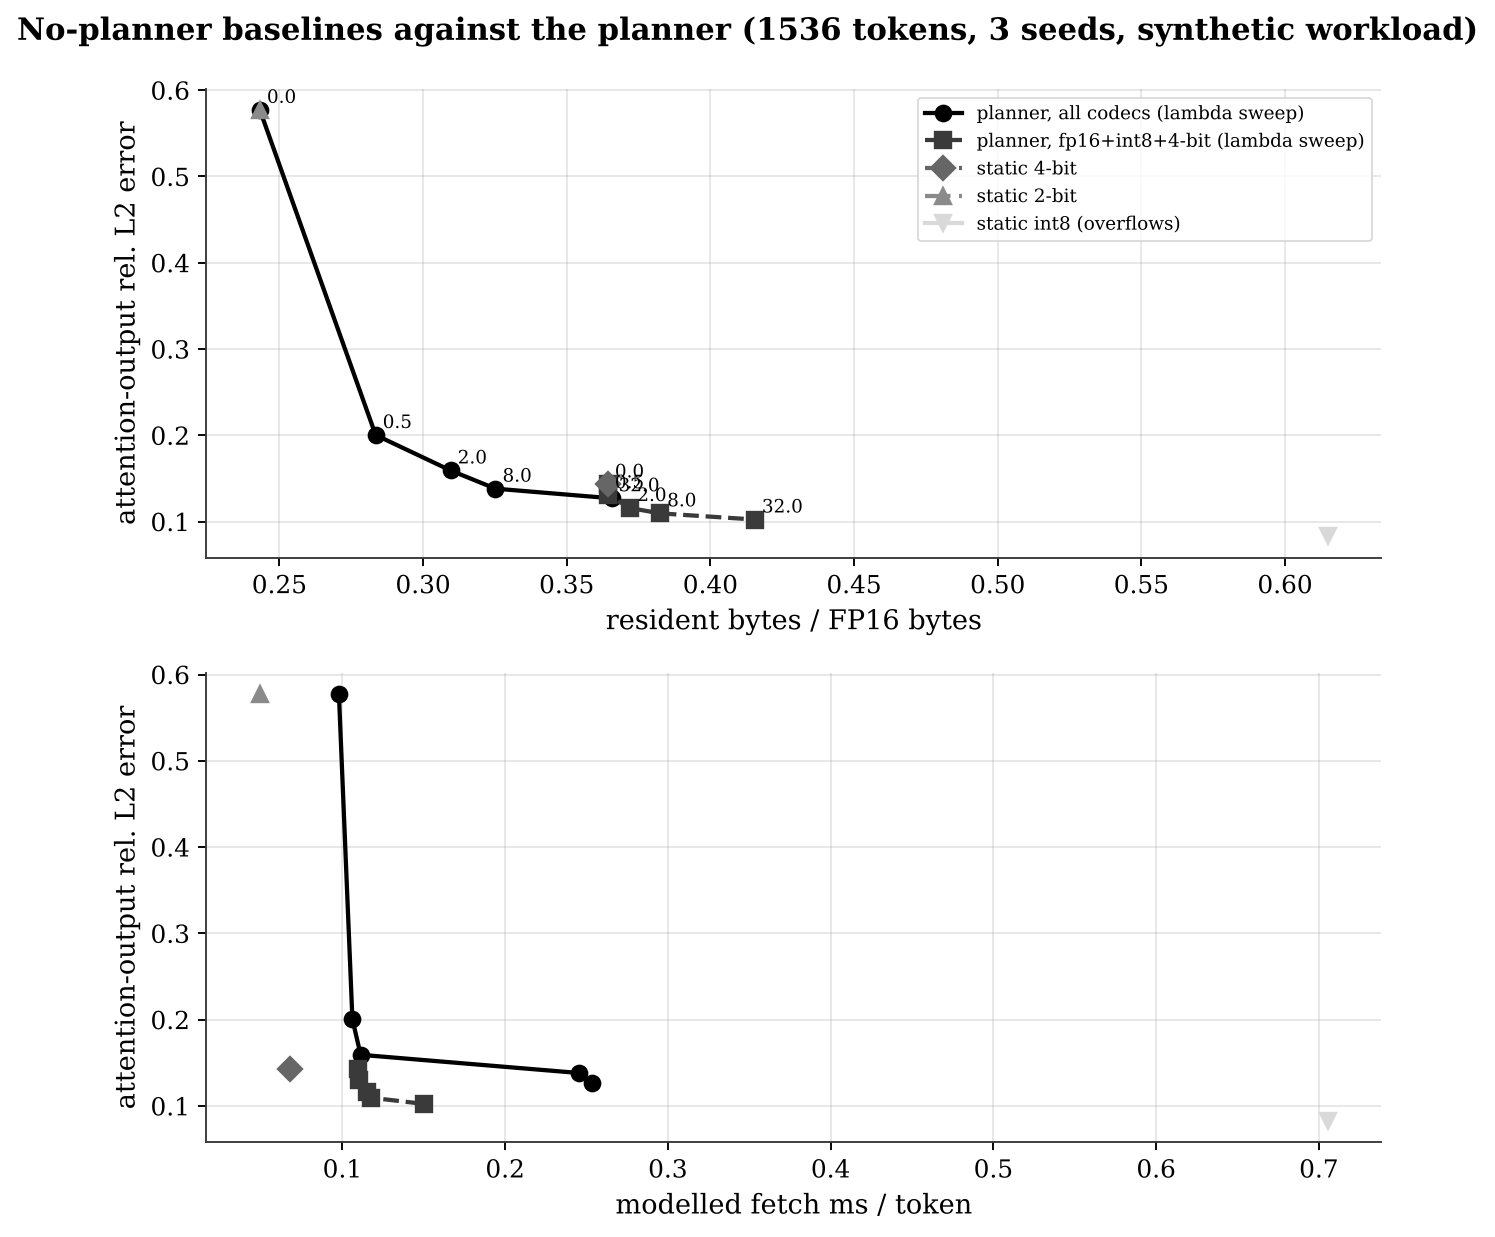
\includegraphics[width=6.27in,height=6.30in,keepaspectratio]{figs/f22_static_vs_planner.png}}
\caption{Error against resident size (left) and against modelled fetch time (right) for the no-planner baselines and for the planner over its λ sweep.}
\end{figure}
The static baseline\index{baseline} places the hottest blocks in the fastest tier\index{tier} with room and stores every unprotected block in one codec\index{codec}. With 4-bit blocks everything fits mostly in DRAM, which is why its modelled fetch time is the lowest (0.068 ms). The planner\index{planner} with INT8\index{INT8} + KIVI\index{KIVI}-4 reaches lower error (0.116–0.131 for λ between 0.5 and 2, against 0.143) at the same residency\index{residency}, but fetches in about 0.11 ms, because the higher-precision blocks it keeps are larger and push other blocks to flash\index{flash}. No setting of λ in the sweep gives both the speed of the static baseline and the lower error. With all codecs enabled the planner can go below the static baseline in memory (0.284–0.310 against 0.364) at higher error. The honest reading is that the planner offers a controllable trade-off between memory, error and fetch time, whereas the static policy is one fixed, simple and fast point on it, and that the planner is not faster than that point in this model.

\subsubsection{Charging the key summaries to the budget (E9)}\label{sec:8_1_2}
{\fontsize{8}{9.5}\selectfont\setlength{\tabcolsep}{3pt}
\begin{longtable}{>{\raggedright\arraybackslash}p{1.42in}>{\raggedright\arraybackslash}p{0.89in}>{\raggedright\arraybackslash}p{0.80in}>{\raggedright\arraybackslash}p{0.80in}>{\raggedright\arraybackslash}p{0.53in}>{\raggedright\arraybackslash}p{0.62in}>{\raggedright\arraybackslash}p{0.53in}}
\caption{Effect of charging the per-block key min/max summaries to the 168 KB budget (1,536 tokens, 5 seeds).}\\
\toprule
\textbf{Variant} & \textbf{Resident incl. summaries / FP16} & \textbf{Overflow, summaries free (B)} & \textbf{Overflow, summaries charged (B)} & \textbf{Dropped} & \textbf{Rel. L2 error} & \textbf{Fetch ms} \\\midrule\endfirsthead
\toprule \textbf{Variant} & \textbf{Resident incl. summaries / FP16} & \textbf{Overflow, summaries free (B)} & \textbf{Overflow, summaries charged (B)} & \textbf{Dropped} & \textbf{Rel. L2 error} & \textbf{Fetch ms} \\\midrule\endhead
\bottomrule\endfoot
UAMM-1 threshold policy & 0.412 ± 0.012 & 0 ± 0 & 0 ± 0 & 1069 ± 16 & 0.618 ± 0.037 & 1.049 ± 0.021 \\
No planner: every block 4-bit & 0.489 ± 0.000 & 0 ± 0 & 7,187 ± 0 & 0 ± 0 & 0.152 ± 0.015 & 0.095 ± 0.005 \\
Planner, INT8 + KIVI-4 & 0.496 ± 0.003 & 0 ± 0 & 3,438 ± 1,007 & 0 ± 0 & 0.127 ± 0.013 & 0.128 ± 0.004 \\
Planner, all codecs & 0.435 ± 0.001 & 0 ± 0 & 0 ± 0 & 0 ± 0 & 0.177 ± 0.018 & 0.124 ± 0.004 \\
\bottomrule
\end{longtable}}
The selection step keeps, for every block, a minimum and a maximum key vector in FP16\index{FP16}: 2 × 64 × 2 = 256 B per block, 24,576 B for 96 blocks, which is 14 \% of the 168 KB budget\index{budget}. The main experiments do not charge this memory. Experiment E9 charges it by shrinking the tier\index{tier} capacities by the same amount (to 0.857 of their size). Under that accounting the INT8\index{INT8} + KIVI\index{KIVI}-4 planner\index{planner} overflows by about 3.4 KB and the all-4-bit baseline\index{baseline} by about 7.2 KB, so the statement that these variants fit the budget holds only if the summaries are free. The all-codec planner still fits, with error 0.177 and fetch time 0.124 ms. Including the summaries, its resident size is 0.435 of FP16, not 0.310. The summaries are also read at every step to rank blocks, a cost that the fetch model does not include.

\subsection{Scaling with context length (E2)}\label{sec:8_2}
{\fontsize{8}{9.5}\selectfont\setlength{\tabcolsep}{3pt}
\begin{longtable}{>{\raggedright\arraybackslash}p{0.78in}>{\raggedright\arraybackslash}p{0.93in}>{\raggedright\arraybackslash}p{1.01in}>{\raggedright\arraybackslash}p{0.93in}>{\raggedright\arraybackslash}p{1.01in}>{\raggedright\arraybackslash}p{1.01in}}
\caption{Context scaling with the 168 KB budget fixed (mean of 3 seeds). UAMM-2 columns use all codecs unless stated. (columns 1 to 5)}\\
\toprule
\textbf{Tokens} & \textbf{Err UAMM-1} & \textbf{Err UAMM-2 (all)} & \textbf{Recall UAMM-1} & \textbf{Recall UAMM-2} & \textbf{Dropped (UAMM-1)} \\\midrule\endfirsthead
\toprule \textbf{Tokens} & \textbf{Err UAMM-1} & \textbf{Err UAMM-2 (all)} & \textbf{Recall UAMM-1} & \textbf{Recall UAMM-2} & \textbf{Dropped (UAMM-1)} \\\midrule\endhead
\bottomrule\endfoot
512 & 0.001 & 0.016 & 0.999 & 0.999 & 0 \\
768 & 0.100 & 0.042 & 0.954 & 0.990 & 245 \\
1024 & 0.241 & 0.071 & 0.881 & 0.976 & 496 \\
1536 & 0.505 & 0.159 & 0.750 & 0.945 & 971 \\
2048 & 0.683 & 0.270 & 0.657 & 0.913 & 1461 \\
3072 & 0.985 & 0.515 & 0.532 & 0.830 & 2469 \\
\bottomrule
\end{longtable}}
{\fontsize{8}{9.5}\selectfont\setlength{\tabcolsep}{3pt}
\begin{longtable}{>{\raggedright\arraybackslash}p{0.86in}>{\raggedright\arraybackslash}p{1.29in}>{\raggedright\arraybackslash}p{1.03in}>{\raggedright\arraybackslash}p{1.03in}>{\raggedright\arraybackslash}p{1.55in}}
\caption{Context scaling with the 168 KB budget fixed (mean of 3 seeds). UAMM-2 columns use all codecs unless stated. (columns 6 to 9)}\\
\toprule
\textbf{Tokens} & \textbf{Resident/FP16 (UAMM-2)} & \textbf{Fetch ms UAMM-1} & \textbf{Fetch ms UAMM-2} & \textbf{Overflow B: INT8+K4 / all} \\\midrule\endfirsthead
\toprule \textbf{Tokens} & \textbf{Resident/FP16 (UAMM-2)} & \textbf{Fetch ms UAMM-1} & \textbf{Fetch ms UAMM-2} & \textbf{Overflow B: INT8+K4 / all} \\\midrule\endhead
\bottomrule\endfoot
512 & 0.538 & 0.473 & 0.035 & 0 / 0 \\
768 & 0.445 & 0.728 & 0.049 & 0 / 0 \\
1024 & 0.376 & 0.846 & 0.072 & 0 / 0 \\
1536 & 0.310 & 0.919 & 0.111 & 0 / 0 \\
2048 & 0.266 & 0.948 & 0.152 & 25,899 / 0 \\
3072 & 0.241 & 0.946 & 0.178 & 132,309 / 28,501 \\
\bottomrule
\end{longtable}}
\begin{figure}[htbp]
\centering
\adjustbox{max width=\linewidth}{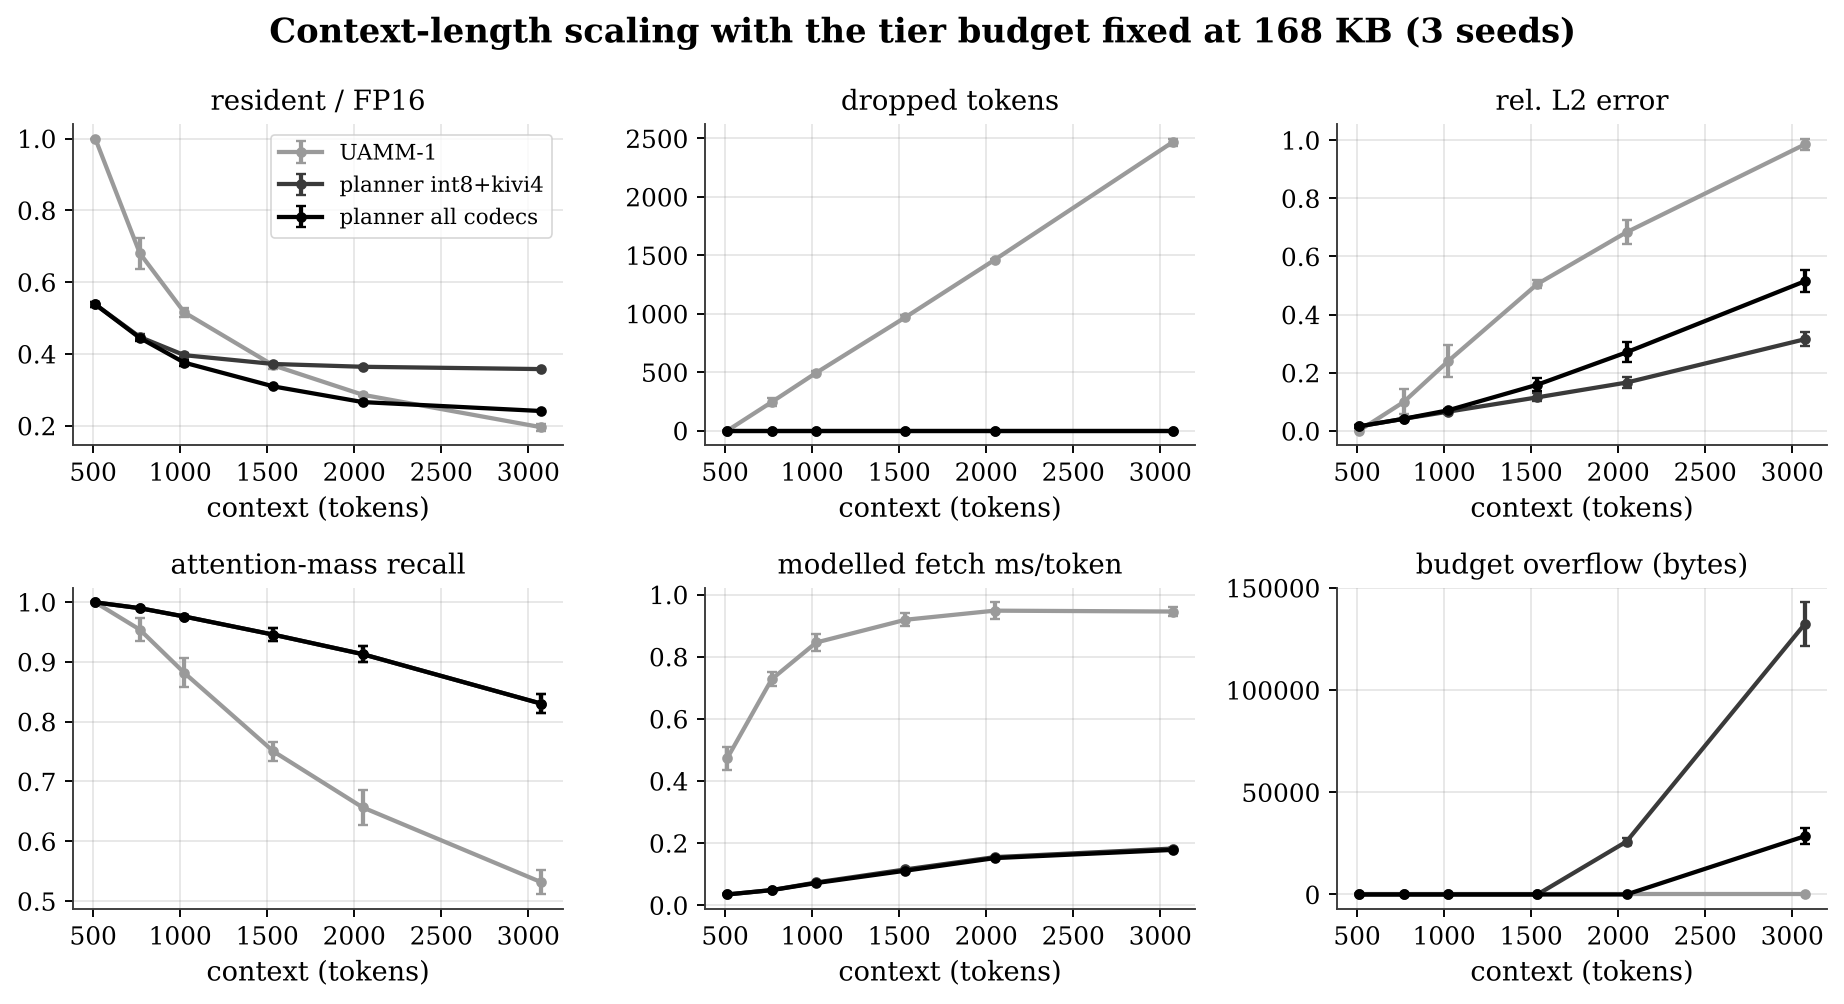
\includegraphics[width=6.27in,height=6.30in,keepaspectratio]{figs/f06_context_scaling.png}}
\caption{Context scaling at a fixed budget. UAMM-1's error and drops grow quickly beyond 768 tokens; UAMM-2 degrades gradually and keeps every token until the budget is exceeded near 3,072 tokens.}
\end{figure}
\begin{itemize}
\item \textbf{Short contexts.} At 512 tokens the cache fits at FP16\index{FP16} (UAMM-1\index{UAMM-1} resident ratio 1.0, error 0.0013). UAMM-2\index{UAMM-2} still compresses (resident 0.538) and is 14× faster in the model (0.035 ms vs 0.473 ms) but incurs a small error (0.016). That is a policy consequence of the cost function: when latency is priced and the quality term is small, the planner\index{planner} lowers precision even without capacity pressure. If the application prefers exactness when memory is available, λ should be raised or compression gated on pressure (Chapter~\ref{sec:12}).
\item \textbf{Medium contexts.} At 1,024 tokens UAMM-1\index{UAMM-1} has dropped 496 tokens (error 0.241, recall\index{recall} 0.882); UAMM-2\index{UAMM-2} holds all tokens with error 0.071 and recall 0.976.
\item \textbf{Long contexts.} At 2,048 tokens UAMM-2\index{UAMM-2} (all codecs) still fits (resident 0.266, error 0.270, recall\index{recall} 0.913). At 3,072 tokens it overflows its budget\index{budget} by 28.5 KB (INT8\index{INT8}+KIVI\index{KIVI}-4 only: 132 KB) and error is 0.515 vs 0.985 for UAMM-1\index{UAMM-1}, which has dropped 2,469 of 3,072 tokens. Beyond this point the fixed budget is simply too small for the data even at 2-bit; opt-in drop or a larger budget would be needed.
\item \textbf{Recall.} Recall falls with context in both systems but for different reasons: in UAMM-1\index{UAMM-1} because tokens are missing, in UAMM-2\index{UAMM-2} because the fixed block budget\index{budget} of 24 covers a shrinking fraction of the history (see E3).
\end{itemize}
\subsection{How many blocks must be read? (E3)}\label{sec:8_3}
{\fontsize{8}{9.5}\selectfont\setlength{\tabcolsep}{3pt}
\begin{longtable}{>{\raggedright\arraybackslash}p{0.93in}>{\raggedright\arraybackslash}p{1.21in}>{\raggedright\arraybackslash}p{1.21in}>{\raggedright\arraybackslash}p{1.21in}>{\raggedright\arraybackslash}p{1.21in}}
\caption{Effect of the attention block budget at 1,536 tokens (mean ± std, 3 seeds).}\\
\toprule
\textbf{Block budget B} & \textbf{Mass recall} & \textbf{Rel. L2 error} & \textbf{Fetch ms / token} & \textbf{Resident / FP16} \\\midrule\endfirsthead
\toprule \textbf{Block budget B} & \textbf{Mass recall} & \textbf{Rel. L2 error} & \textbf{Fetch ms / token} & \textbf{Resident / FP16} \\\midrule\endhead
\bottomrule\endfoot
4 & 0.568 ± 0.013 & 1.101 ± 0.016 & 0.036 ± 0.003 & 0.269 ± 0.001 \\
8 & 0.744 ± 0.017 & 0.663 ± 0.015 & 0.062 ± 0.002 & 0.272 ± 0.003 \\
12 & 0.841 ± 0.019 & 0.443 ± 0.027 & 0.087 ± 0.001 & 0.277 ± 0.001 \\
16 & 0.895 ± 0.017 & 0.308 ± 0.022 & 0.098 ± 0.003 & 0.285 ± 0.002 \\
24 & 0.945 ± 0.011 & 0.159 ± 0.023 & 0.111 ± 0.002 & 0.310 ± 0.001 \\
32 & 0.966 ± 0.007 & 0.101 ± 0.008 & 0.132 ± 0.004 & 0.337 ± 0.004 \\
48 & 0.986 ± 0.003 & 0.070 ± 0.002 & 0.278 ± 0.024 & 0.376 ± 0.002 \\
\bottomrule
\end{longtable}}
\begin{figure}[htbp]
\centering
\adjustbox{max width=\linewidth}{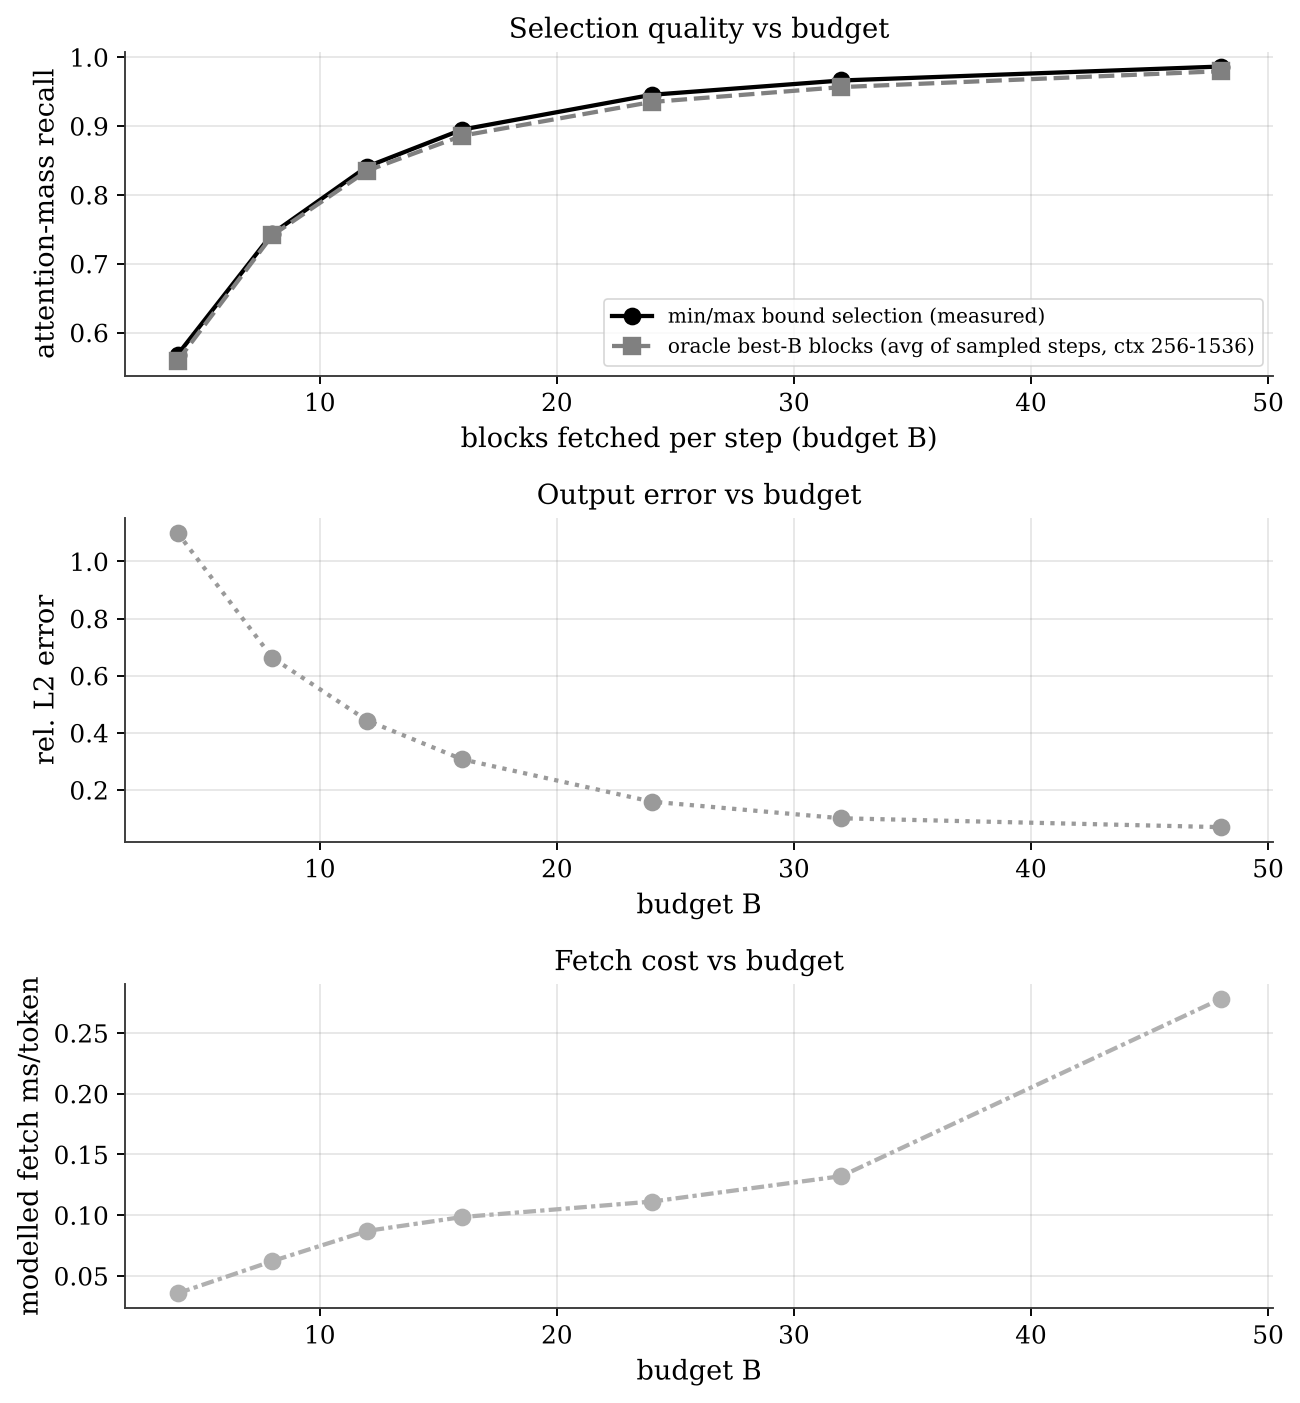
\includegraphics[width=6.27in,height=6.30in,keepaspectratio]{figs/f07_budget_sweep.png}}
\caption{Block budget sweep. Left: recall of the min/max-bound selector versus the oracle choice of the B heaviest blocks averaged over sampled steps (indicative; the system also reads the protected blocks). Middle and right: error and fetch cost.}
\end{figure}
Selecting 24 blocks (about a quarter of the roughly 96 blocks at 1,536 tokens) retains 94.5 \% of the attention mass with an error of 0.159; 48 blocks reach 98.6 \% at a cost that is 2.5× higher (0.278 ms vs 0.111 ms) because more blocks are fetched from slower tiers. The marginal return of a block falls quickly, as the sorted block mass predicts. Note the interaction with residency\index{residency}: a larger budget\index{budget} reads many cold blocks, which pushes the planner\index{planner} to keep more of them in higher precision (resident 0.376 at B=48 vs 0.310 at B=24).

\subsection{Sensitivity of the planner and the importance signal (E4)}\label{sec:8_4}
\subsubsection{The quality weight λ}\label{sec:8_4_1}
{\fontsize{8}{9.5}\selectfont\setlength{\tabcolsep}{3pt}
\begin{longtable}{>{\raggedright\arraybackslash}p{0.52in}>{\raggedright\arraybackslash}p{1.03in}>{\raggedright\arraybackslash}p{1.03in}>{\raggedright\arraybackslash}p{1.03in}>{\raggedright\arraybackslash}p{1.03in}>{\raggedright\arraybackslash}p{1.03in}}
\caption{Effect of the quality weight λ at 1,536 tokens (3 seeds).}\\
\toprule
\textbf{λ} & \textbf{Resident / FP16} & \textbf{Rel. L2 error} & \textbf{Fetch ms / token} & \textbf{Flash reads} & \textbf{Migrations} \\\midrule\endfirsthead
\toprule \textbf{λ} & \textbf{Resident / FP16} & \textbf{Rel. L2 error} & \textbf{Fetch ms / token} & \textbf{Flash reads} & \textbf{Migrations} \\\midrule\endhead
\bottomrule\endfoot
0.0 & 0.243 ± 0.000 & 0.577 ± 0.020 & 0.098 ± 0.003 & 724 ± 38 & 573 ± 7 \\
0.25 & 0.264 ± 0.002 & 0.289 ± 0.016 & 0.101 ± 0.001 & 763 ± 16 & 610 ± 18 \\
0.5 & 0.284 ± 0.002 & 0.200 ± 0.028 & 0.106 ± 0.003 & 836 ± 44 & 631 ± 11 \\
1.0 & 0.295 ± 0.001 & 0.181 ± 0.031 & 0.108 ± 0.003 & 860 ± 48 & 639 ± 17 \\
2.0 & 0.310 ± 0.001 & 0.159 ± 0.023 & 0.111 ± 0.002 & 908 ± 37 & 630 ± 15 \\
4.0 & 0.315 ± 0.003 & 0.152 ± 0.025 & 0.197 ± 0.031 & 2189 ± 455 & 567 ± 6 \\
8.0 & 0.325 ± 0.003 & 0.138 ± 0.012 & 0.245 ± 0.003 & 2912 ± 45 & 567 ± 24 \\
16.0 & 0.343 ± 0.004 & 0.134 ± 0.013 & 0.237 ± 0.004 & 2792 ± 60 & 614 ± 20 \\
32.0 & 0.366 ± 0.006 & 0.127 ± 0.009 & 0.253 ± 0.007 & 3036 ± 102 & 726 ± 53 \\
\bottomrule
\end{longtable}}
\begin{figure}[htbp]
\centering
\adjustbox{max width=\linewidth}{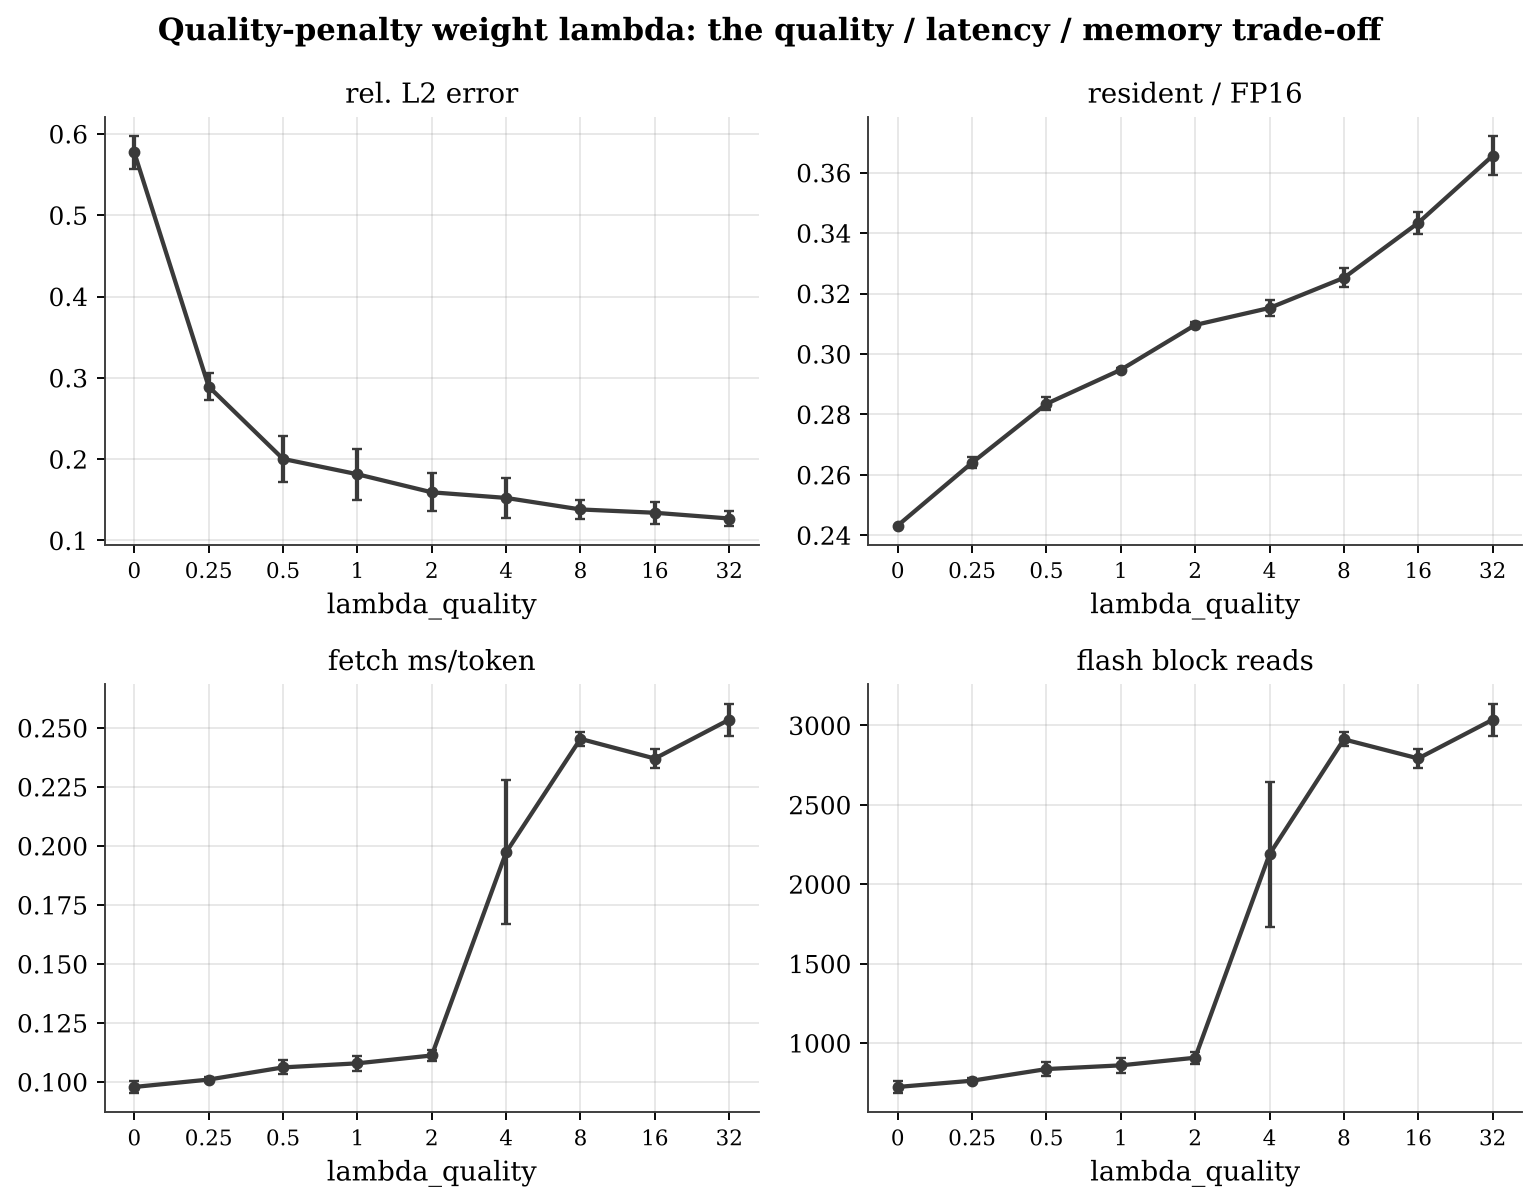
\includegraphics[width=6.27in,height=6.30in,keepaspectratio]{figs/f08_lambda_sweep.png}}
\caption{Effect of λ on error, memory, fetch latency and flash reads.}
\end{figure}
As λ rises the planner\index{planner} protects quality: error falls from 0.577 at λ = 0 (maximum compression, resident 0.243) to 0.127 at λ = 32, at the price of larger residency\index{residency} (0.366). Latency is not monotone: up to λ = 2 fetch time is nearly flat at about 0.10–0.11 ms, then jumps to 0.20–0.25 ms at λ ≥ 4 and flash\index{flash} reads triple. The cause, visible in the planner's cost, is that choosing larger encodings for a block can push other blocks out of DRAM into flash, whose fixed 100 µs access cost dwarfs the transfer savings. The default λ = 2 sits at the knee: the error is within 25 \% of the best seen (0.159 vs 0.127) while fetch time is roughly half that of λ ≥ 4 (0.111 ms against 0.20–0.25 ms).

\subsubsection{Hysteresis, residency and replanning interval}\label{sec:8_4_2}
{\fontsize{8}{9.5}\selectfont\setlength{\tabcolsep}{3pt}
\begin{longtable}{>{\raggedright\arraybackslash}p{0.93in}>{\raggedright\arraybackslash}p{0.85in}>{\raggedright\arraybackslash}p{0.85in}>{\raggedright\arraybackslash}p{1.02in}>{\raggedright\arraybackslash}p{1.02in}>{\raggedright\arraybackslash}p{1.02in}}
\caption{Hysteresis margin (3 seeds).}\\
\toprule
\textbf{Hysteresis margin} & \textbf{Migrations} & \textbf{Re-encodes} & \textbf{Resident / FP16} & \textbf{Rel. L2 error} & \textbf{Fetch ms / token} \\\midrule\endfirsthead
\toprule \textbf{Hysteresis margin} & \textbf{Migrations} & \textbf{Re-encodes} & \textbf{Resident / FP16} & \textbf{Rel. L2 error} & \textbf{Fetch ms / token} \\\midrule\endhead
\bottomrule\endfoot
0.0 & 1871 ± 45 & 247 ± 3 & 0.286 ± 0.004 & 0.208 ± 0.030 & 0.112 ± 0.002 \\
0.1 & 784 ± 27 & 240 ± 3 & 0.292 ± 0.004 & 0.181 ± 0.027 & 0.111 ± 0.004 \\
0.25 & 630 ± 15 & 226 ± 2 & 0.310 ± 0.001 & 0.159 ± 0.023 & 0.111 ± 0.002 \\
0.5 & 593 ± 14 & 188 ± 4 & 0.359 ± 0.006 & 0.111 ± 0.013 & 0.116 ± 0.003 \\
1.0 & 463 ± 26 & 180 ± 3 & 0.373 ± 0.005 & 0.110 ± 0.013 & 0.115 ± 0.003 \\
\bottomrule
\end{longtable}}
\begin{figure}[htbp]
\centering
\adjustbox{max width=\linewidth}{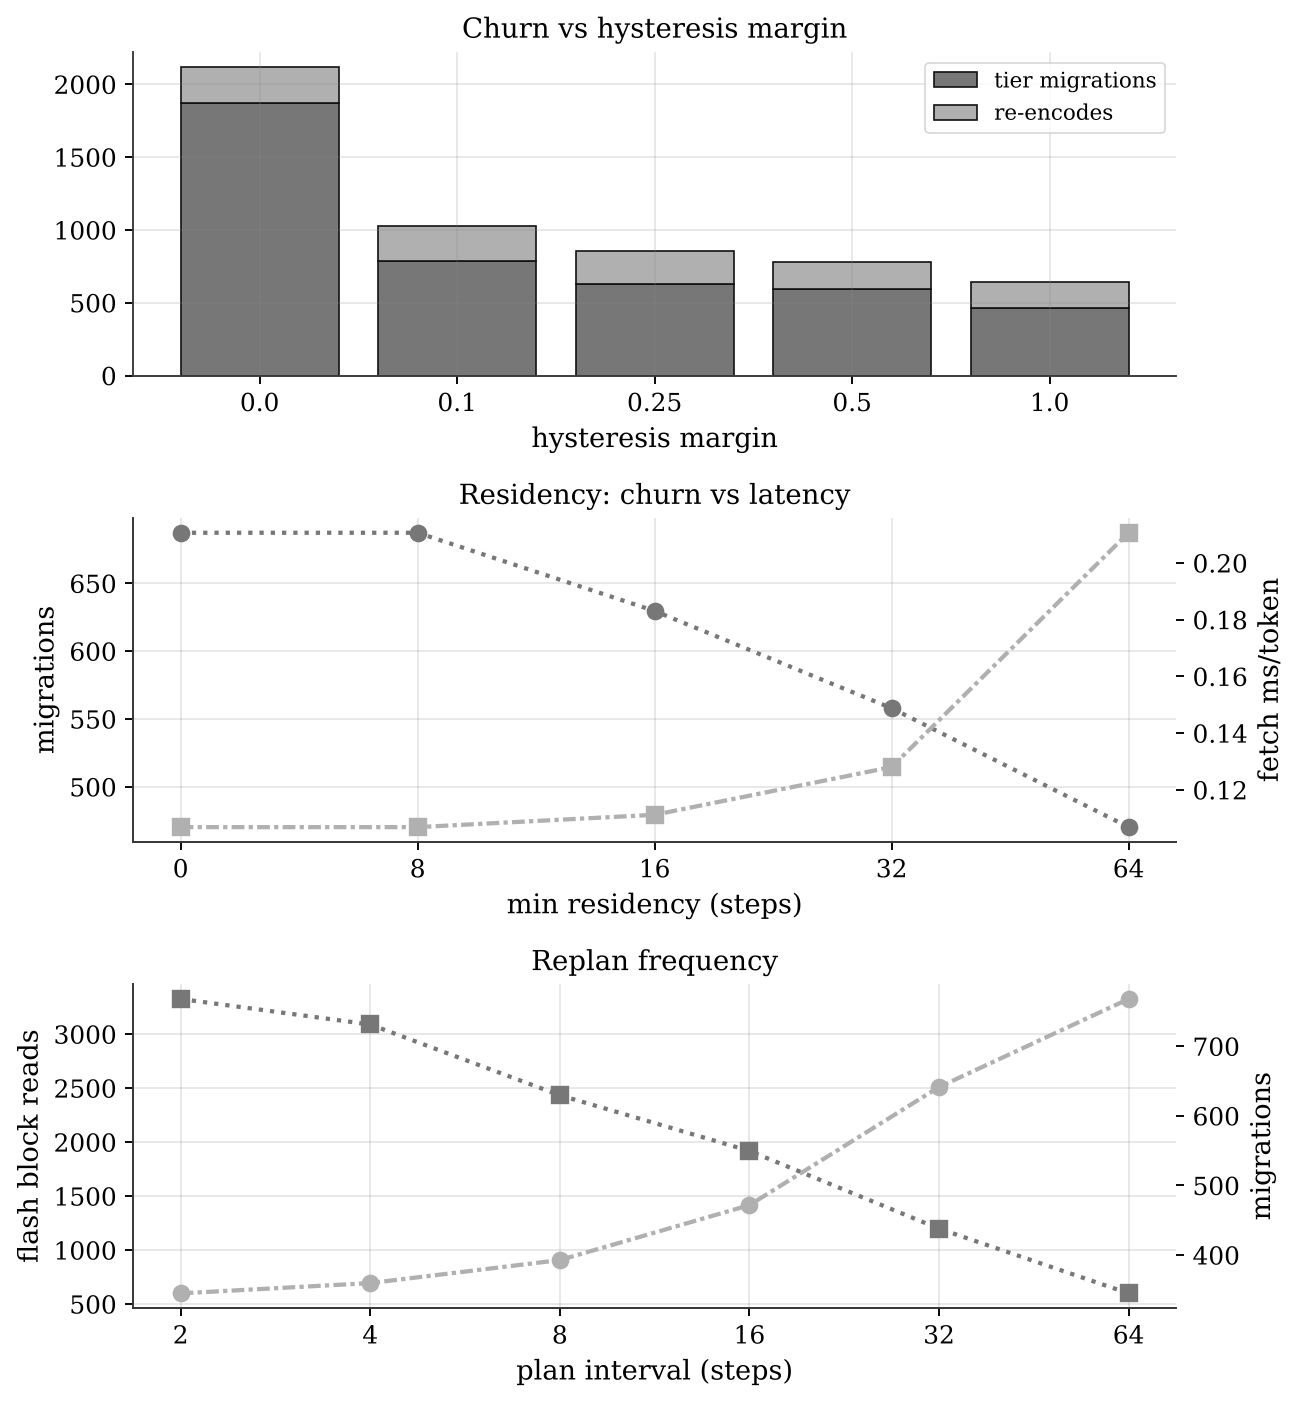
\includegraphics[width=6.27in,height=6.30in,keepaspectratio]{figs/f10_stability_knobs.png}}
\caption{Left: churn versus hysteresis margin. Middle: minimum residency. Right: planning interval.}
\end{figure}
Without hysteresis\index{hysteresis} (margin 0) the planner\index{planner} performs 1,871 migrations; with the default margin of 0.25 it performs 630, a reduction of 66 \% at essentially unchanged fetch time (0.1118 vs 0.1112 ms). The trade-off is that a larger margin also suppresses precision demotions (re-encodes fall from 247 to 180), so residency\index{residency} grows (0.286 to 0.373) and error falls (0.208 to 0.110). Hysteresis is therefore both a churn limiter and a quality-conservative bias.

The minimum-residency rule has no effect below 16 steps because the planning interval is 8 (identical rows for 0 and 8): residency\index{residency} is only meaningful when it exceeds the interval. At 64 steps migrations fall to 470, but fetch time doubles (0.211 ms) and flash\index{flash} reads reach 2,384, because blocks that have become hot cannot be promoted in time. Likewise the replanning interval: planning every 2 steps gives 599 flash reads and 0.090 ms but 768 migrations, whereas every 64 steps gives 3,326 flash reads and 0.272 ms with only 345 migrations. The planner\index{planner} must keep up with the changes in attention focus; the cost of keeping up is the planning work itself, which is why the hardware sweep scorer\index{sweep scorer} exists.

\subsubsection{H2O decay, aggregation and block size}\label{sec:8_4_3}
{\fontsize{8}{9.5}\selectfont\setlength{\tabcolsep}{3pt}
\begin{longtable}{>{\raggedright\arraybackslash}p{0.90in}>{\raggedright\arraybackslash}p{1.26in}>{\raggedright\arraybackslash}p{1.26in}>{\raggedright\arraybackslash}p{1.26in}>{\raggedright\arraybackslash}p{1.08in}}
\caption{H2O decay (3 seeds).}\\
\toprule
\textbf{H2O decay} & \textbf{Resident / FP16} & \textbf{Rel. L2 error} & \textbf{Fetch ms / token} & \textbf{Re-encodes} \\\midrule\endfirsthead
\toprule \textbf{H2O decay} & \textbf{Resident / FP16} & \textbf{Rel. L2 error} & \textbf{Fetch ms / token} & \textbf{Re-encodes} \\\midrule\endhead
\bottomrule\endfoot
0.5 & 0.285 ± 0.003 & 0.202 ± 0.018 & 0.112 ± 0.002 & 244 ± 3 \\
0.8 & 0.285 ± 0.003 & 0.202 ± 0.018 & 0.111 ± 0.002 & 244 ± 2 \\
0.9 & 0.286 ± 0.003 & 0.202 ± 0.018 & 0.112 ± 0.002 & 244 ± 2 \\
0.95 & 0.310 ± 0.001 & 0.159 ± 0.023 & 0.111 ± 0.002 & 226 ± 2 \\
0.98 & 0.329 ± 0.005 & 0.135 ± 0.010 & 0.108 ± 0.002 & 210 ± 1 \\
0.995 & 0.368 ± 0.004 & 0.114 ± 0.009 & 0.110 ± 0.002 & 173 ± 2 \\
\bottomrule
\end{longtable}}
A longer memory of attention (decay 0.995) makes the planner\index{planner} more conservative about compressing blocks that were important at some point: error falls from 0.202 (decay ≤ 0.9) to 0.114 and residency\index{residency} rises from 0.285 to 0.368, at essentially constant fetch time (0.110–0.112 ms). Decay therefore moves the system along the same memory-versus-quality axis as λ but at no latency cost in this configuration. Mean and sum aggregation are equivalent (sum is normalised by the same percentile; blocks have equal size); max aggregation gives slightly lower residency (0.301) and similar error (0.162).

{\fontsize{8}{9.5}\selectfont\setlength{\tabcolsep}{3pt}
\begin{longtable}{>{\raggedright\arraybackslash}p{1.00in}>{\raggedright\arraybackslash}p{1.00in}>{\raggedright\arraybackslash}p{1.00in}>{\raggedright\arraybackslash}p{1.00in}>{\raggedright\arraybackslash}p{0.84in}>{\raggedright\arraybackslash}p{0.84in}}
\caption{Block size (3 seeds; block budget scaled to keep ≈384 non-protected tokens fetched).}\\
\toprule
\textbf{Block size (tokens)} & \textbf{Resident / FP16} & \textbf{Rel. L2 error} & \textbf{Fetch ms / token} & \textbf{Migrations} & \textbf{Overflow (B)} \\\midrule\endfirsthead
\toprule \textbf{Block size (tokens)} & \textbf{Resident / FP16} & \textbf{Rel. L2 error} & \textbf{Fetch ms / token} & \textbf{Migrations} & \textbf{Overflow (B)} \\\midrule\endhead
\bottomrule\endfoot
8 & 0.387 ± 0.008 & 0.110 ± 0.014 & 0.216 ± 0.009 & 1652 ± 86 & 0 ± 0 \\
16 & 0.310 ± 0.001 & 0.159 ± 0.023 & 0.111 ± 0.002 & 630 ± 15 & 0 ± 0 \\
32 & 0.264 ± 0.003 & 0.219 ± 0.036 & 0.063 ± 0.002 & 275 ± 19 & 0 ± 0 \\
64 & 0.264 ± 0.013 & 0.341 ± 0.010 & 0.038 ± 0.002 & 121 ± 6 & 14336 ± 0 \\
\bottomrule
\end{longtable}}
Block size is a three-way trade-off. Small blocks (8 tokens) isolate hot tokens well, giving the lowest error (0.110), but have more metadata, more migrations (1,652) and much higher fetch time (0.216 ms, since each block pays a fixed latency). Large blocks (64) cut migrations to 121 and fetch time to 0.038 ms but raise error to 0.341 and overflow the budget\index{budget} by 14 KB: a block must be placed and compressed as a unit, so a few hot tokens drag a whole large block into a fast tier\index{tier}. A block of 16 tokens is a reasonable compromise and also fits the hardware tables.

\subsection{Memory budget (E5)}\label{sec:8_5}
{\fontsize{6.5}{8.0}\selectfont\setlength{\tabcolsep}{3pt}
\begin{longtable}{>{\raggedright\arraybackslash}p{0.74in}>{\raggedright\arraybackslash}p{0.57in}>{\raggedright\arraybackslash}p{0.57in}>{\raggedright\arraybackslash}p{0.57in}>{\raggedright\arraybackslash}p{0.57in}>{\raggedright\arraybackslash}p{0.57in}>{\raggedright\arraybackslash}p{0.57in}>{\raggedright\arraybackslash}p{0.57in}>{\raggedright\arraybackslash}p{0.65in}}
\caption{Memory-budget sweep at 1,536 tokens (mean of 3 seeds).}\\
\toprule
\textbf{Budget} & \textbf{UAMM-1 resident} & \textbf{UAMM-1 dropped} & \textbf{UAMM-1 error} & \textbf{UAMM-1 fetch ms} & \textbf{UAMM-2 resident} & \textbf{UAMM-2 error} & \textbf{UAMM-2 fetch ms} & \textbf{UAMM-2 overflow B} \\\midrule\endfirsthead
\toprule \textbf{Budget} & \textbf{UAMM-1 resident} & \textbf{UAMM-1 dropped} & \textbf{UAMM-1 error} & \textbf{UAMM-1 fetch ms} & \textbf{UAMM-2 resident} & \textbf{UAMM-2 error} & \textbf{UAMM-2 fetch ms} & \textbf{UAMM-2 overflow B} \\\midrule\endhead
\bottomrule\endfoot
×0.5 (84 KB) & 0.219 & 1200 & 0.855 & 0.757 & 0.288 & 0.220 & 0.301 & 33,109 \\
×0.75 (126 KB) & 0.299 & 1077 & 0.661 & 1.001 & 0.293 & 0.180 & 0.141 & 0 \\
×1.0 (168 KB) & 0.368 & 971 & 0.505 & 0.919 & 0.310 & 0.159 & 0.111 & 0 \\
×1.5 (252 KB) & 0.521 & 736 & 0.280 & 0.733 & 0.323 & 0.131 & 0.099 & 0 \\
×2.0 (336 KB) & 0.625 & 576 & 0.171 & 0.612 & 0.330 & 0.115 & 0.088 & 0 \\
×3.0 (504 KB) & 0.830 & 261 & 0.086 & 0.502 & 0.324 & 0.152 & 0.049 & 0 \\
\bottomrule
\end{longtable}}
\begin{figure}[htbp]
\centering
\adjustbox{max width=\linewidth}{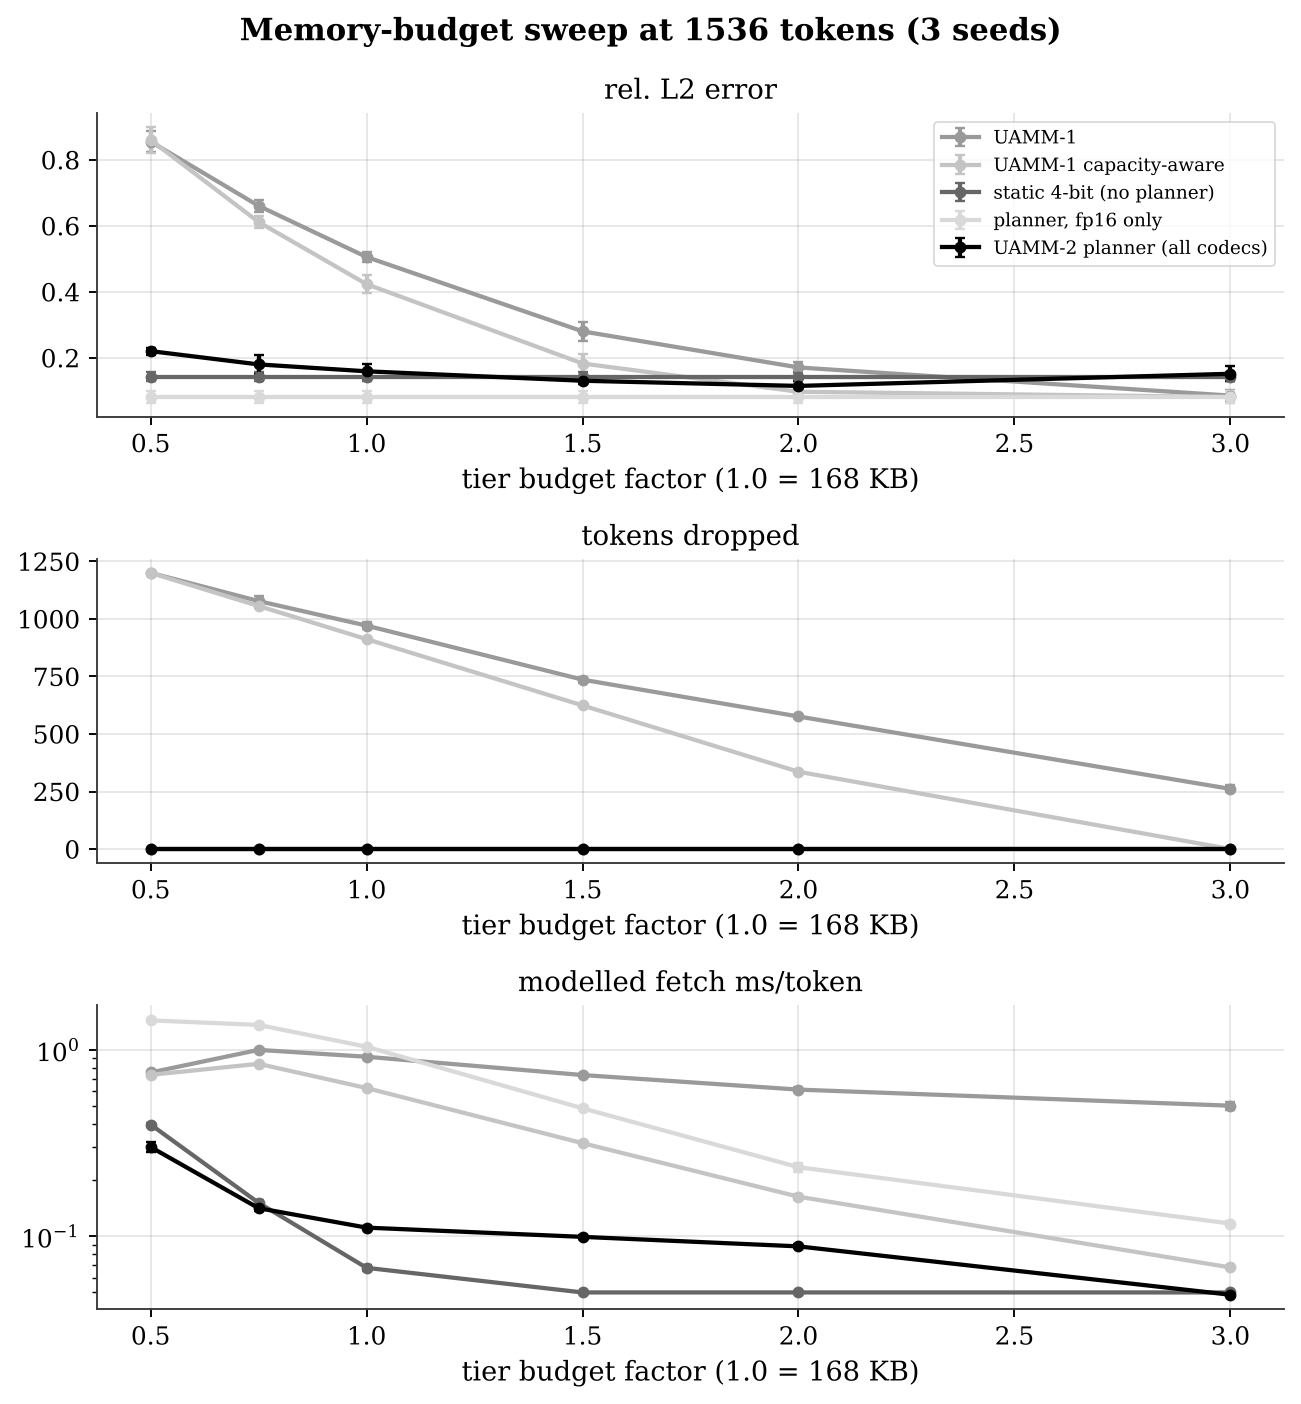
\includegraphics[width=6.27in,height=6.30in,keepaspectratio]{figs/f12_capacity_sweep.png}}
\caption{Budget sweep. UAMM-1 needs roughly three times the baseline budget to bring error below 0.09 and still drops 261 tokens; UAMM-2 reaches comparable error without drops at much smaller budgets.}
\end{figure}
\begin{itemize}
\item \textbf{Equal-quality comparison with UAMM-1.} UAMM-2\index{UAMM-2} at ×0.75 of the budget\index{budget} (126 KB) has error 0.180 and drops nothing; the original UAMM-1\index{UAMM-1} needs ×2.0 (336 KB) to reach a similar error (0.171) and still drops 576 tokens. This comparison is against the original threshold rule only; the fairer baselines below narrow it.
\item \textbf{Infeasibility.} At ×0.5 (84 KB) UAMM-2\index{UAMM-2} overflows by 33 KB (the data do not fit even at its most compressed); UAMM-1\index{UAMM-1} does not report overflow but drops 1,200 tokens and has error 0.855.
\item \textbf{Non-monotonic quality.} UAMM-2\index{UAMM-2}'s error is 0.115 at ×2.0 but 0.152 at ×3.0, even though more memory is available. At ×3.0 flash\index{flash} is almost unused (3 reads) and the planner\index{planner} spends the headroom on speed (fetch 0.049 ms vs 0.088 ms) by choosing smaller encodings. This is the cost function working as designed, but it is a reminder that the optimiser, not the budget\index{budget}, decides the trade-off, and that a quality floor (Chapter~\ref{sec:12}) is needed to guarantee monotonic behaviour.
\end{itemize}
\textbf{Fairer baselines across budgets.} The same sweep was repeated for three baselines: the capacity-aware UAMM-1\index{UAMM-1}, the FP16\index{FP16}-only planner\index{planner} and the planner-free 4-bit policy.

{\fontsize{6.5}{8.0}\selectfont\setlength{\tabcolsep}{3pt}
\begin{longtable}{>{\raggedright\arraybackslash}p{0.53in}>{\raggedright\arraybackslash}p{0.75in}>{\raggedright\arraybackslash}p{0.48in}>{\raggedright\arraybackslash}p{0.75in}>{\raggedright\arraybackslash}p{0.48in}>{\raggedright\arraybackslash}p{0.75in}>{\raggedright\arraybackslash}p{0.48in}>{\raggedright\arraybackslash}p{0.70in}>{\raggedright\arraybackslash}p{0.48in}}
\caption{Baselines across memory budgets at 1,536 tokens (3 seeds).}\\
\toprule
\textbf{Budget} & \textbf{UAMM-1 cap.-aware: dropped} & \textbf{error} & \textbf{All 4-bit: overflow B} & \textbf{error} & \textbf{FP16 planner: overflow B} & \textbf{error} & \textbf{UAMM-2: overflow B} & \textbf{error} \\\midrule\endfirsthead
\toprule \textbf{Budget} & \textbf{UAMM-1 cap.-aware: dropped} & \textbf{error} & \textbf{All 4-bit: overflow B} & \textbf{error} & \textbf{FP16 planner: overflow B} & \textbf{error} & \textbf{UAMM-2: overflow B} & \textbf{error} \\\midrule\endhead
\bottomrule\endfoot
×0.5 & 1200 ± 0 & 0.860 ± 0.040 & 67,925 ± 2,465 & 0.143 ± 0.013 & 331,776 ± 0 & 0.081 ± 0.018 & 33,109 ± 3,205 & 0.220 ± 0.010 \\
×0.75 & 1056 ± 0 & 0.611 ± 0.019 & 24,064 ± 0 & 0.143 ± 0.013 & 298,325 ± 1,931 & 0.081 ± 0.018 & 0 ± 0 & 0.180 ± 0.028 \\
×1.0 & 912 ± 0 & 0.423 ± 0.028 & 0 ± 0 & 0.143 ± 0.013 & 256,683 ± 965 & 0.081 ± 0.018 & 0 ± 0 & 0.159 ± 0.023 \\
×1.5 & 624 ± 0 & 0.183 ± 0.029 & 0 ± 0 & 0.143 ± 0.013 & 192,512 ± 0 & 0.081 ± 0.018 & 0 ± 0 & 0.131 ± 0.010 \\
×2.0 & 336 ± 0 & 0.097 ± 0.019 & 0 ± 0 & 0.143 ± 0.013 & 124,245 ± 2,554 & 0.081 ± 0.018 & 0 ± 0 & 0.115 ± 0.016 \\
×3.0 & 0 ± 0 & 0.081 ± 0.018 & 0 ± 0 & 0.143 ± 0.013 & 0 ± 0 & 0.081 ± 0.018 & 0 ± 0 & 0.152 ± 0.023 \\
\bottomrule
\end{longtable}}
\begin{itemize}
\item \textbf{Generous budgets remove the advantage.} FP16\index{FP16} for all 1,536 tokens needs 393 KB, which is 2.3× the baseline\index{baseline} budget\index{budget}. At ×3.0 (504 KB) the FP16-only planner\index{planner} fits with zero overflow and the lowest error (0.081), and the capacity-aware UAMM-1\index{UAMM-1} keeps every token at FP16 with error 0.081 and 0.068 ms, which beats UAMM-2\index{UAMM-2} at that budget (error 0.152). The large gain of UAMM-2 over UAMM-1 in the main experiment depends on a budget that is 2.3× smaller than the data.
\item \textbf{The original UAMM-1 deletes even when memory is ample.} At ×3.0 it still drops 261 tokens, because a block may only go to its target tier\index{tier} or a slower one. This is a defect of the threshold rule, not of capacity.
\item \textbf{Tighter budgets favour the planner.} At ×0.75 the all-4-bit policy overflows by 24 KB, whereas the planner\index{planner} fits (error 0.180) by using 2-bit for cold blocks. At ×0.5 neither fits (overflow 68 KB against 33 KB). Above ×1.0 the 4-bit policy fits and is simpler and faster.
\end{itemize}
\subsubsection{Which codecs should be enabled? (E5b)}\label{sec:8_5_1}
{\fontsize{8}{9.5}\selectfont\setlength{\tabcolsep}{3pt}
\begin{longtable}{>{\raggedright\arraybackslash}p{1.58in}>{\raggedright\arraybackslash}p{1.05in}>{\raggedright\arraybackslash}p{1.05in}>{\raggedright\arraybackslash}p{1.05in}>{\raggedright\arraybackslash}p{1.05in}}
\caption{Codec-set study at 1,536 tokens (3 seeds).}\\
\toprule
\textbf{Enabled codecs} & \textbf{Resident / FP16} & \textbf{Rel. L2 error} & \textbf{Fetch ms / token} & \textbf{Overflow (B)} \\\midrule\endfirsthead
\toprule \textbf{Enabled codecs} & \textbf{Resident / FP16} & \textbf{Rel. L2 error} & \textbf{Fetch ms / token} & \textbf{Overflow (B)} \\\midrule\endhead
\bottomrule\endfoot
FP16 only & 1.000 ± 0.000 & 0.081 ± 0.018 & 1.040 ± 0.007 & 256,683 ± 965 \\
FP16 + INT8 & 0.606 ± 0.000 & 0.083 ± 0.018 & 0.460 ± 0.014 & 104,704 ± 0 \\
+ KIVI-4 & 0.372 ± 0.002 & 0.116 ± 0.013 & 0.115 ± 0.003 & 0 ± 0 \\
+ KIVI-2 (all) & 0.310 ± 0.001 & 0.159 ± 0.023 & 0.111 ± 0.002 & 0 ± 0 \\
FP16 + KIVI-4 only & 0.364 ± 0.000 & 0.132 ± 0.013 & 0.112 ± 0.002 & 0 ± 0 \\
FP16 + KIVI-2 only & 0.346 ± 0.015 & 0.308 ± 0.018 & 0.475 ± 0.012 & 0 ± 0 \\
\bottomrule
\end{longtable}}
\begin{itemize}
\item \textbf{Feasibility needs 4-bit.} FP16\index{FP16} alone (overflow 257 KB) and FP16+INT8\index{INT8} (overflow 105 KB) cannot fit the budget\index{budget}; a 4-bit codec\index{codec} is the first that does.
\item \textbf{KIVI-4 alone is competitive.} FP16\index{FP16} + KIVI\index{KIVI}-4 reaches 0.364 resident at error 0.132 and fetch 0.112 ms, close to the full set on speed with lower error than the full set (0.159); the full set saves a further 15 \% memory.
\item \textbf{KIVI-2 alone is a poor choice.} With only FP16\index{FP16} and KIVI\index{KIVI}-2 available the planner\index{planner} reaches 0.346 resident, but error doubles (0.308) and fetch time is 4× worse (0.475 ms, about 6,200 flash\index{flash} reads). The reason is structural: the tier\index{tier} rules force warm and cold storage to hold a 2-bit block, and without intermediate precision the planner cannot place blocks that matter more at reasonable cost.
\item \textbf{Entropy coding gave no benefit here.} Results with and without zlib variants are identical, which means the planner\index{planner} never preferred a \texttt{z} variant. On the synthetic data, zlib on already quantised random-like values saves almost nothing (Table of codec\index{codec} sizes in Section~\ref{sec:5}). Real KV tensors have more redundancy and the result may differ; this is an open question rather than a conclusion.
\end{itemize}
\subsection{Codec micro-benchmarks (E7)}\label{sec:8_7}
{\fontsize{8}{9.5}\selectfont\setlength{\tabcolsep}{3pt}
\begin{longtable}{>{\raggedright\arraybackslash}p{0.72in}>{\raggedright\arraybackslash}p{1.17in}>{\raggedright\arraybackslash}p{1.26in}>{\raggedright\arraybackslash}p{1.26in}>{\raggedright\arraybackslash}p{1.35in}}
\caption{Key quantisation axis: relative squared error of keys only (200 random 16 × 64 blocks per row).}\\
\toprule
\textbf{Bits} & \textbf{Outlier channels} & \textbf{Per-channel keys} & \textbf{Per-token keys} & \textbf{Per-token / per-channel} \\\midrule\endfirsthead
\toprule \textbf{Bits} & \textbf{Outlier channels} & \textbf{Per-channel keys} & \textbf{Per-token keys} & \textbf{Per-token / per-channel} \\\midrule\endhead
\bottomrule\endfoot
2-bit & without & 1.07e-01 & 2.02e-01 & 1.9× \\
2-bit & with & 1.07e-01 & 5.81e-01 & 5.4× \\
4-bit & without & 4.22e-03 & 8.04e-03 & 1.9× \\
4-bit & with & 4.18e-03 & 2.17e-02 & 5.2× \\
8-bit & without & 1.47e-05 & 2.79e-05 & 1.9× \\
8-bit & with & 1.47e-05 & 7.52e-05 & 5.1× \\
\bottomrule
\end{longtable}}
Quantising keys per channel is always better, by a factor of 1.9 without outlier channels and 5.2–5.4× when four of the 64 channels are six times larger, which agrees with the design choice reported for KIVI\index{KIVI}. Error rises by roughly 25× from 4-bit to 2-bit for the same block (0.0052 → 0.130 in the codec\index{codec} table), which is why 2-bit is treated as the tier\index{tier} of last resort, although with the default settings the planner\index{planner} still assigns it to about half of the blocks (Section~\ref{sec:8_1}).

\subsection{Final placement map}\label{sec:8_9}
\begin{figure}[htbp]
\centering
\adjustbox{max width=\linewidth}{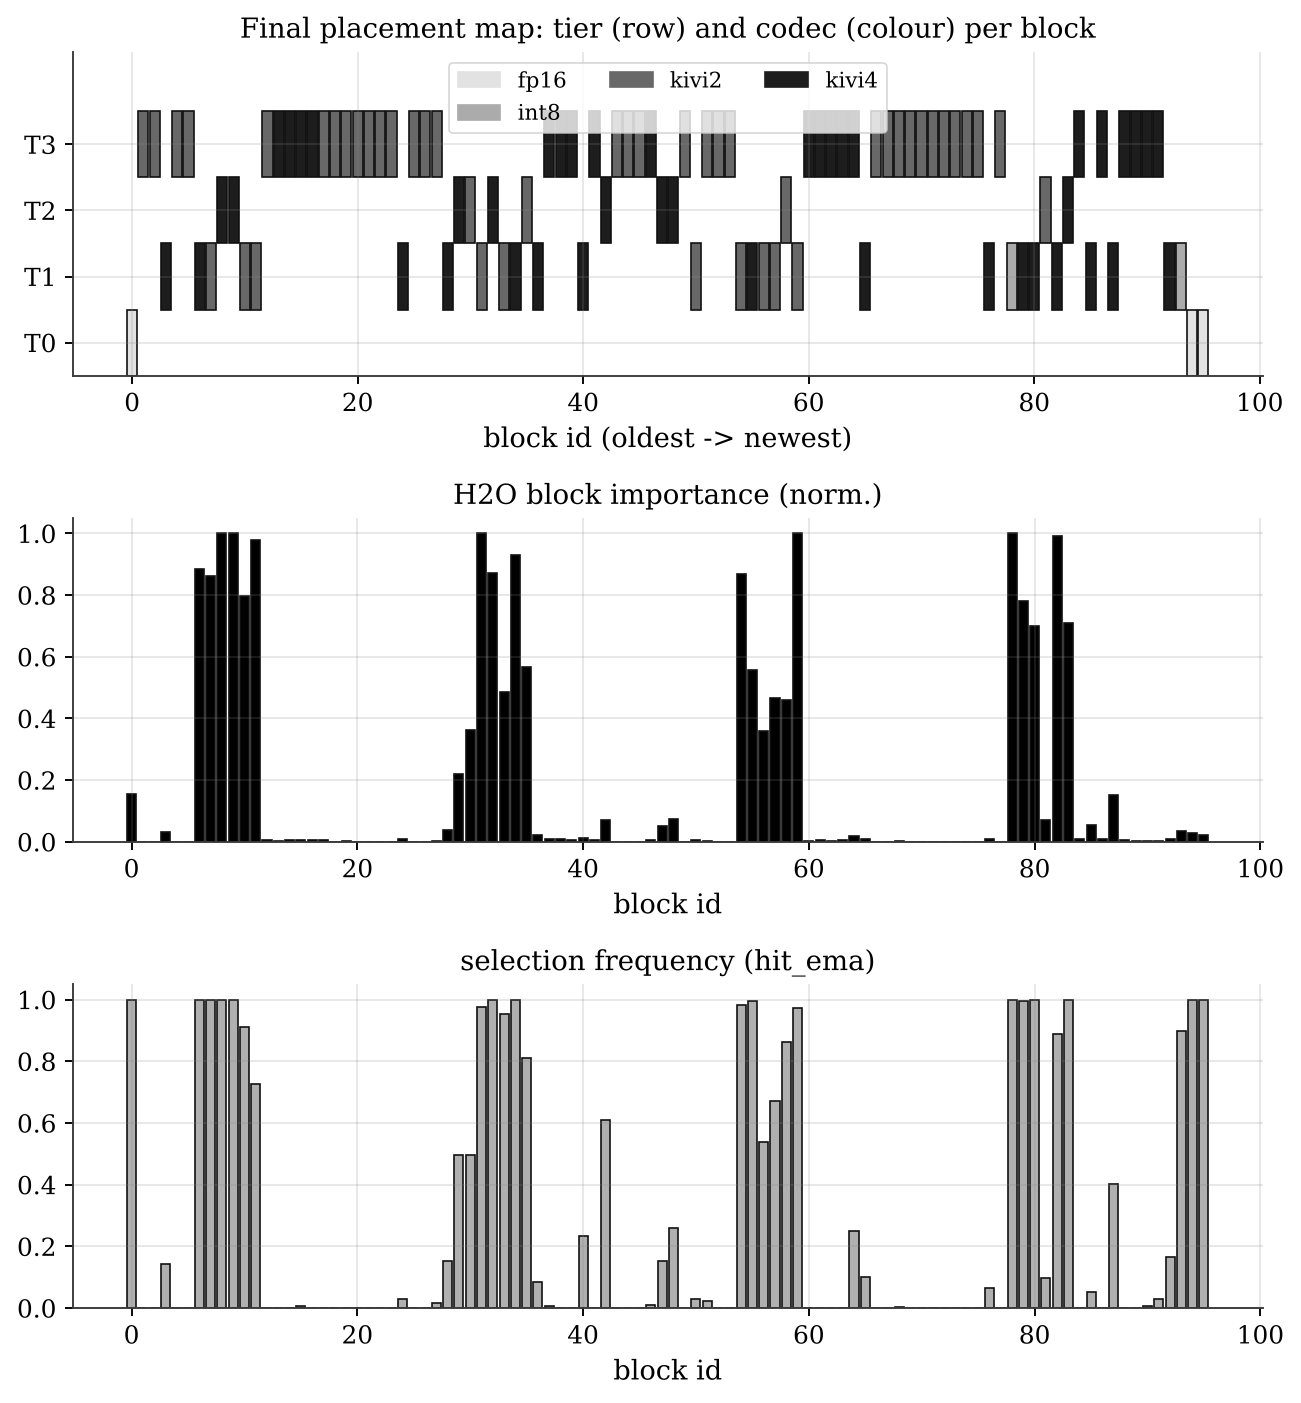
\includegraphics[width=6.27in,height=6.30in,keepaspectratio]{figs/f19_final_placement.png}}
\caption{State of the cache at step 1,536: tier (row) and codec (colour) of every block, with block importance and selection frequency. Older, low-importance blocks occupy flash at 2- or 4-bit; recent blocks are in T0 at FP16.}
\end{figure}
The final state has 96 blocks. Tier T0 holds only FP16\index{FP16} blocks (protected sink and recent window). T1 holds 28 blocks (mainly 4-bit), T2 holds 12 and the flash\index{flash} tier\index{tier} T3 holds 53, all at 4 or 2 bits. No block in T0 or T1 is FP16 beyond the protected set: at this budget\index{budget} the planner\index{planner} has chosen to spend bytes on keeping everything rather than on keeping any unprotected block uncompressed.

\subsection{Summary of the simulation findings}\label{sec:8_10}
{\fontsize{8}{9.5}\selectfont\setlength{\tabcolsep}{3pt}
\begin{longtable}{>{\raggedright\arraybackslash}p{3.03in}>{\raggedright\arraybackslash}p{3.03in}}
\caption{Key findings from the simulations.}\\
\toprule
\textbf{Finding} & \textbf{Evidence} \\\midrule\endfirsthead
\toprule \textbf{Finding} & \textbf{Evidence} \\\midrule\endhead
\bottomrule\endfoot
A joint (tier, codec) choice lets a tight budget hold every token without deleting & E1: 0 dropped tokens against 973; but a one-codec 4-bit baseline does this too (E1, E10) \\
The planner buys accuracy and robustness to tight budgets, not speed & E10: error 0.116–0.131 against 0.143 at equal memory, fetch 0.11 against 0.068 ms; E5: all-4-bit overflows at ×0.75, planner does not \\
The size of the advantage over UAMM-1 depends on how tight the budget is & E5: at ×3.0 FP16 alone fits with error 0.081 \\
Counting the key summaries changes which variants fit & E9: INT8 + KIVI-4 and all-4-bit overflow; all-codec planner fits (0.435 resident) \\
Quality is bounded and tunable & E4: λ and decay move error between 0.11 and 0.58 along a memory axis \\
Selective attention delivers most of the saving & E3: 24 of \textasciitilde{}96 blocks gives 94.5 \% mass recall \\
Hysteresis removes most churn & E4: 1,871 → 630 migrations with the default margin \\
Replanning cadence matters for flash traffic & E4: 599 → 3,326 flash reads from interval 2 → 64 \\
Budget exhaustion is graceful, not catastrophic & E2: gradual error growth; overflow reported, not hidden \\
Some behaviour is non-obvious and needs a floor or a policy & E5: non-monotonic error at 3× memory; E2: compression when memory is ample \\
\bottomrule
\end{longtable}}
\section{Hardware Results: RTL Simulation, Waveforms and Verification}\label{sec:9}
This chapter presents the results for the three Verilog modules: how they were verified, the waveforms recorded during the testbench runs, the lint and mutation results and the synthesis statistics. Every figure showing signals was rendered directly from the value-change-dump (VCD) files written by the Verilator\index{Verilator} simulations (\texttt{docs/\allowbreak{}wave/\allowbreak{}trace\_\allowbreak{}\allowbreak{}*.\allowbreak{}vcd}).

\begin{calloutbox}{How to read the waveform figures}
The figures are screenshots of the GTKWave\index{GTKWave} waveform viewer (GTK 3 build, run in a virtual X display). Each opens one of the VCD dumps written by Verilator\index{Verilator} from the testbenches in \texttt{hw/\allowbreak{}tb} (rerun with \texttt{+trace}), with the signals, radix, zoom range and marker placed by a Tcl script kept in \texttt{docs/\allowbreak{}gtkwave/\allowbreak{}}. Buses are shown in hexadecimal or decimal as indicated in the signal values; the vertical line is the marker.

\end{calloutbox}
\begin{calloutbox}{Scope of the hardware}
The sweep scorer\index{sweep scorer} implements the weighted score of the original UAMM-1\index{UAMM-1} (importance, recency and frequency with the weights 154/64/38 and two thresholds). It does not implement the planner\index{planner}'s utility cost, so the hardware and the UAMM-2\index{UAMM-2} software policy are not yet the same function; Scope 13 in Chapter~\ref{sec:12} describes the change.

The codec\index{codec} module quantises 8-bit group values with a reciprocal supplied by firmware. The software codecs start from FP16\index{FP16}, so a front stage that produces the 8-bit values is still missing.

All checks are simulations in Verilator\index{Verilator} against Python golden models. There is no place-and-route result, no timing and no power figure.

\end{calloutbox}
\subsection{Verification method}\label{sec:9_1}
\begin{enumerate}
\item \textbf{Golden models.} \texttt{uamm2/\allowbreak{}hwmodel.\allowbreak{}py} re-implements each module's integer arithmetic line for line.
\item \textbf{Vector generation.} The same file writes stimulus and expected-output hex files (\texttt{hw/\allowbreak{}vectors/\allowbreak{}*.\allowbreak{}hex}), including directed boundary cases and random cases.
\item \textbf{Self-checking testbenches.} Each testbench reads the vectors, drives the module, compares every output with the expectation and prints \texttt{PASS} or \texttt{FAIL} with a count.
\item \textbf{Verilator\index{Verilator} 5.} \texttt{make -C hw test} builds and runs all three benches with timing support; \texttt{+trace} additionally dumps a VCD.
\item \textbf{Lint.} \texttt{verilator --lint-only -Wall} on every module.
\item \textbf{Mutation testing.} Twelve single-fault variants of the RTL are generated automatically; the regression must fail for every one.
\item \textbf{Logic synthesis check.} Yosys\index{Yosys} \texttt{synth} with \texttt{check -assert} confirms the designs elaborate to generic gates with no inferred latches.
\end{enumerate}
\subsection{Sweep scorer}\label{sec:9_2}
The scorer test applies four metadata datasets of 64 blocks, each swept at four pressure levels (0, 242, 243, 255), which gives 16 sweeps; a further sweep exercises restart behaviour (17 in total). Dataset 0 is a set of directed boundary cases: for each of the scores 0, 1, 88, 89, 90, 173, 174, 175, 254 and 255 a metadata word is generated whose weighted score equals that value, once unprotected and once protected, followed by corner cases (all zeros, all 255, single maxima) and random fill. The other three datasets are random with a 20 \% chance of the \texttt{protected} bit.

\begin{figure}[htbp]
\centering
\adjustbox{max width=\linewidth}{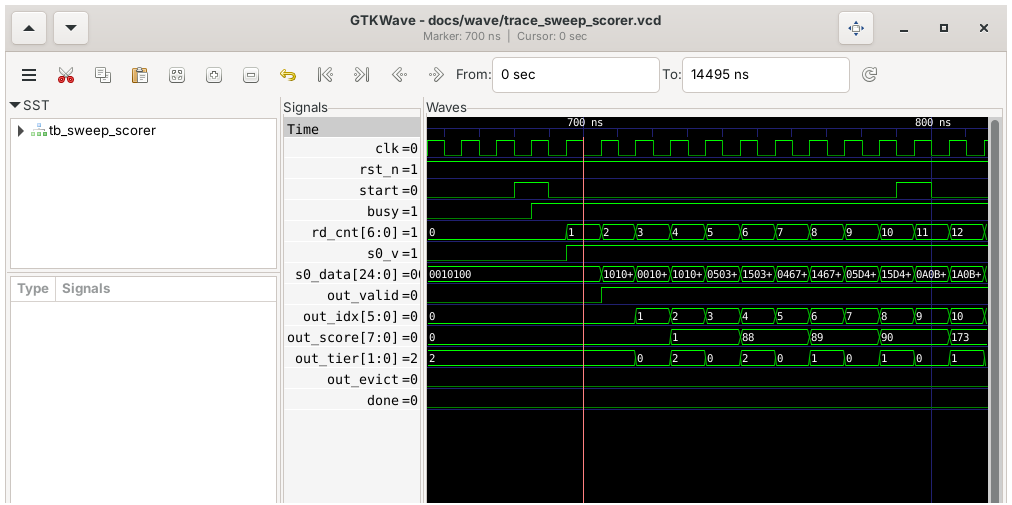
\includegraphics[width=6.27in,height=6.30in,keepaspectratio]{figs/g01_scorer_start.png}}
\caption{Sweep start. start is asserted for one clock; busy rises on the next edge; the read counter then increments once per cycle. s0\_\allowbreak{}data shows the metadata words read from the SRAM; the results appear two cycles later as out\_\allowbreak{}valid with the block index, score and tier.}
\end{figure}
The first results are the directed boundary cases, which makes the figure self-explanatory: block 0 has score 0 and tier\index{tier} 2 (cold) because it is unprotected; block 1 has the same metadata with \texttt{protected} set and is forced to tier 0; block 2 has score 1; blocks 4 and 5 have score 88 (just below the warm threshold of 89, cold when unprotected); blocks 6 and 7 have score 89 (exactly at the warm threshold: warm when unprotected, hot when protected); blocks 8 and 9 have score 90; block 10 has score 173 (one below the hot threshold: warm). The alternation of tier values 2, 0, 2, 0, 2, 0, 1, 0, 1, 0, 1 is the pair-wise unprotected/protected pattern.

\begin{figure}[htbp]
\centering
\adjustbox{max width=\linewidth}{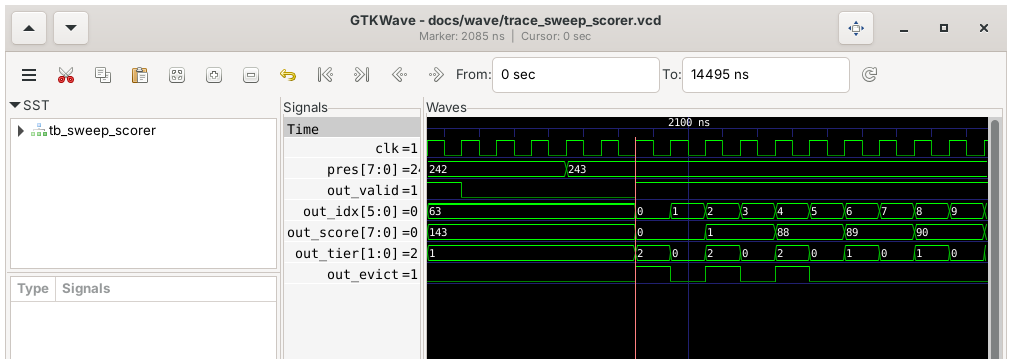
\includegraphics[width=6.27in,height=6.30in,keepaspectratio]{figs/g03_scorer_evict.png}}
\caption{Eviction under pressure. The pressure latched for the sweep changes from 242 to 243; in the sweep at 243, out\_\allowbreak{}evict is raised for blocks 0, 2 and 4 (unprotected, score below 89) and not for the protected blocks or for blocks 6 and 7 (score 89).}
\end{figure}
This is the behaviour the UAMM-1\index{UAMM-1} RTL got wrong (it ignored \texttt{protected}) and the main reason for the boundary vectors: at pressure 242 no block is flagged for eviction; at 243 exactly the unprotected blocks whose score is below 89 are flagged.

\begin{figure}[htbp]
\centering
\adjustbox{max width=\linewidth}{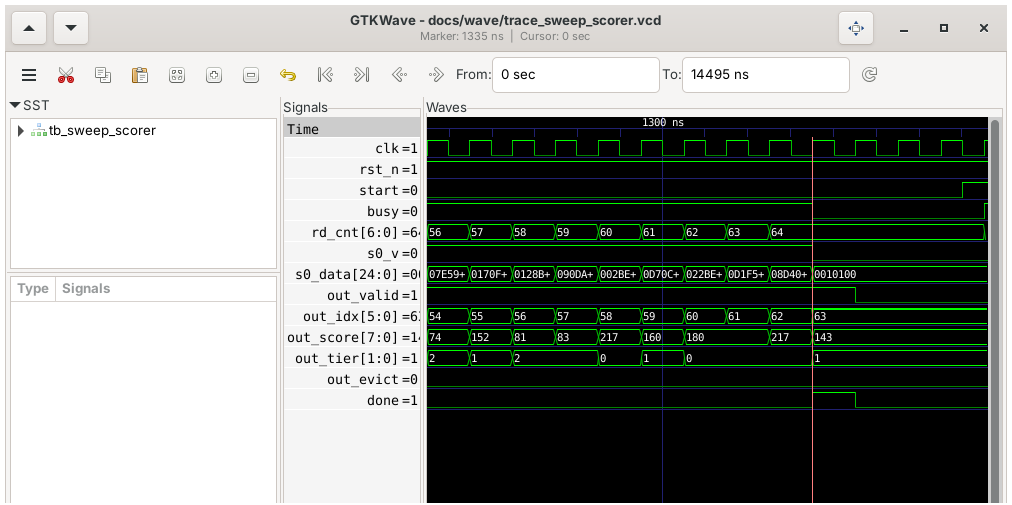
\includegraphics[width=6.27in,height=6.30in,keepaspectratio]{figs/g02_scorer_done.png}}
\caption{End of a sweep. The read counter reaches 64 and busy falls; the last result (block 63) is emitted one cycle later together with the done pulse. A new start can follow immediately.}
\end{figure}
The latency is as designed: for NBLK = 64 a sweep produces its last result NBLK + 3 cycles after \texttt{start}, and it sustains one block per cycle. At a 100 MHz clock a 64-block sweep takes under 0.7 µs; for 4,096 blocks it would take under 41 µs, so the sweep is cheap compared with the planning interval of several decode steps. (These are cycle counts from the simulation multiplied by an assumed clock, not timing-closure results.)

\begin{figure}[htbp]
\centering
\adjustbox{max width=\linewidth}{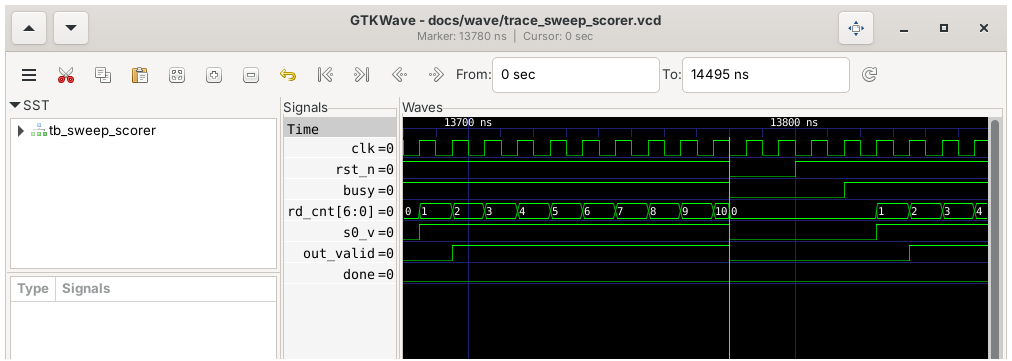
\includegraphics[width=6.27in,height=6.30in,keepaspectratio]{figs/g04_scorer_reset.png}}
\caption{Asynchronous reset in the middle of a sweep. rst\_\allowbreak{}n is pulled low; busy, s0\_\allowbreak{}v and out\_\allowbreak{}valid drop immediately, the read counter returns to zero and a later start begins a clean sweep.}
\end{figure}
{\fontsize{8}{9.5}\selectfont\setlength{\tabcolsep}{3pt}
\begin{longtable}{>{\raggedright\arraybackslash}p{3.91in}>{\raggedright\arraybackslash}p{1.03in}>{\raggedright\arraybackslash}p{1.03in}}
\caption{Sweep scorer results.}\\
\toprule
\textbf{Check} & \textbf{Count} & \textbf{Result} \\\midrule\endfirsthead
\toprule \textbf{Check} & \textbf{Count} & \textbf{Result} \\\midrule\endhead
\bottomrule\endfoot
Sweeps (4 datasets × 4 pressures + restart) & 17 & PASS \\
Total per-block comparisons (score, tier, evict, index, valid) & 1,088 & PASS \\
\texttt{start} while busy ignored & directed & PASS \\
Reset in the middle of a sweep & directed & PASS \\
\bottomrule
\end{longtable}}
\subsection{Codec pipeline}\label{sec:9_3}
The quantiser and dequantiser testbench feeds 400 vectors of 16 lanes. The vectors are produced in four modes in rotation: full-range random, narrow range around a random centre, constant group (range zero) and extremes (0, 1, 254, 255). Further variations set the zero point inside the data or deliberately \textbf{below} the true minimum (stale statistics), which exercises the clamp at code 15. The testbench checks both the 16 packed 4-bit codes and the 16 dequantised bytes.

\begin{figure}[htbp]
\centering
\adjustbox{max width=\linewidth}{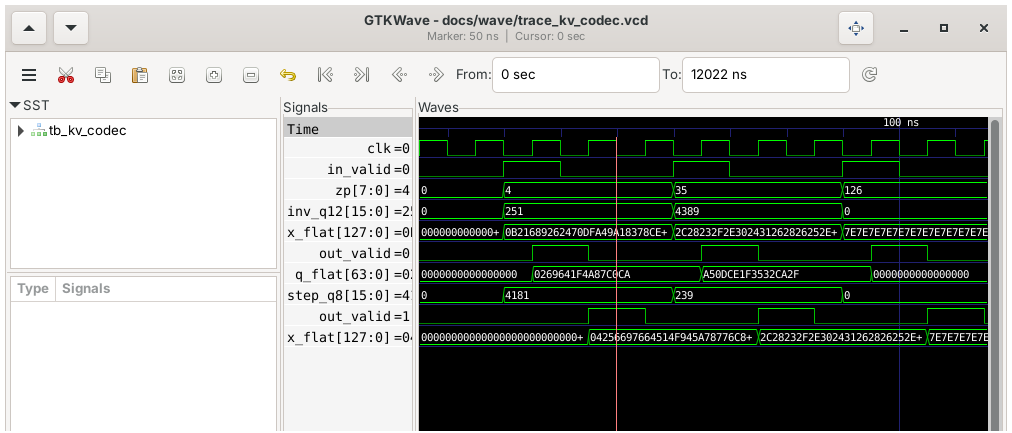
\includegraphics[width=6.27in,height=6.30in,keepaspectratio]{figs/g05_codec_pipeline.png}}
\caption{Two vectors and a constant group through uamm\_\allowbreak{}kv\_\allowbreak{}quant4 and uamm\_\allowbreak{}kv\_\allowbreak{}dequant4. x\_\allowbreak{}flat is the 128-bit input; q\_\allowbreak{}flat is the packed result one cycle after in\_\allowbreak{}valid; the dequantiser is fed the code vector and step and produces x' one cycle later.}
\end{figure}
The third vector in the figure is the constant group (\texttt{inv\_\allowbreak{}\allowbreak{}q12 = 0}, \texttt{step\_\allowbreak{}\allowbreak{}q8 = 0}): all lanes are \texttt{7e}, every code is zero and the dequantiser reproduces \texttt{7e} exactly, as the model predicts. The first two vectors have non-trivial ranges (parameters 251 and 4,389 for inv\_\allowbreak{}q12), show the one-cycle latency of each stage, and match the expected nibble words.

{\fontsize{8}{9.5}\selectfont\setlength{\tabcolsep}{3pt}
\begin{longtable}{>{\raggedright\arraybackslash}p{3.91in}>{\raggedright\arraybackslash}p{1.03in}>{\raggedright\arraybackslash}p{1.03in}}
\caption{Codec results.}\\
\toprule
\textbf{Check} & \textbf{Count} & \textbf{Result} \\\midrule\endfirsthead
\toprule \textbf{Check} & \textbf{Count} & \textbf{Result} \\\midrule\endhead
\bottomrule\endfoot
Codec vectors (quantiser and dequantiser outputs) & 400 & PASS \\
\bottomrule
\end{longtable}}
\subsection{Block table}\label{sec:9_4}
The block-table testbench performs 6,000 random operations (writes, lookups, and the occasional same-cycle read-and-write to one address) and compares every lookup with a behavioural reference table. It also checks that the valid bits are cleared by reset and that a read in the same cycle as a write returns the old entry.

\begin{figure}[htbp]
\centering
\adjustbox{max width=\linewidth}{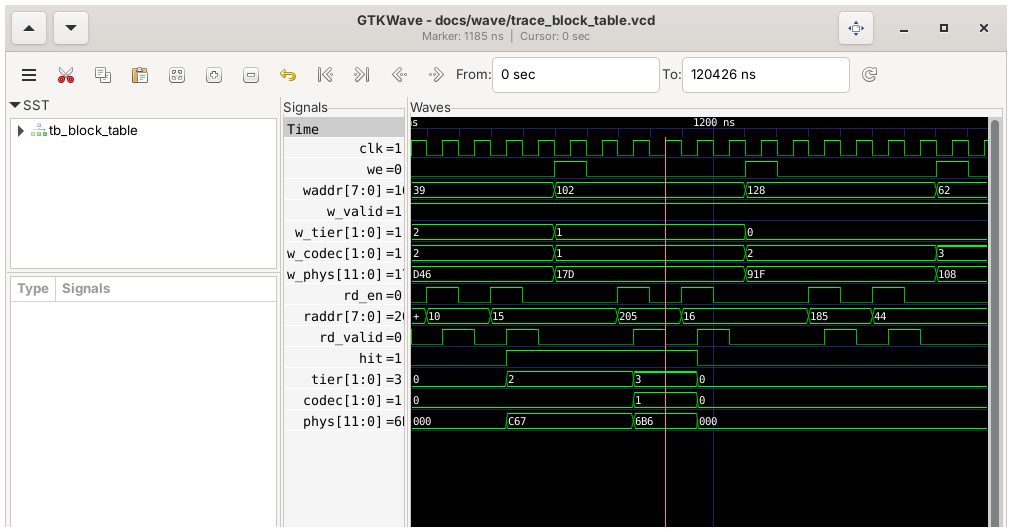
\includegraphics[width=6.27in,height=6.30in,keepaspectratio]{figs/g06_block_table.png}}
\caption{Random updates and lookups. we pulses write \{tier, codec, phys\} to the address on waddr; rd\_\allowbreak{}en pulses start a lookup whose result (hit, tier, codec, phys) appears one cycle later through rd\_\allowbreak{}valid. A lookup of a never-written address returns hit = 0; a hit returns the stored fields.}
\end{figure}
{\fontsize{8}{9.5}\selectfont\setlength{\tabcolsep}{3pt}
\begin{longtable}{>{\raggedright\arraybackslash}p{3.91in}>{\raggedright\arraybackslash}p{1.03in}>{\raggedright\arraybackslash}p{1.03in}}
\caption{Block-table results.}\\
\toprule
\textbf{Check} & \textbf{Count} & \textbf{Result} \\\midrule\endfirsthead
\toprule \textbf{Check} & \textbf{Count} & \textbf{Result} \\\midrule\endhead
\bottomrule\endfoot
Writes & 3,049 & PASS \\
Reads & 2,971 & PASS \\
Reads that hit & 2,313 & PASS \\
\bottomrule
\end{longtable}}
\subsection{Regression, lint and mutation results}\label{sec:9_5}
\begin{figure}[htbp]
\centering
\adjustbox{max width=\linewidth}{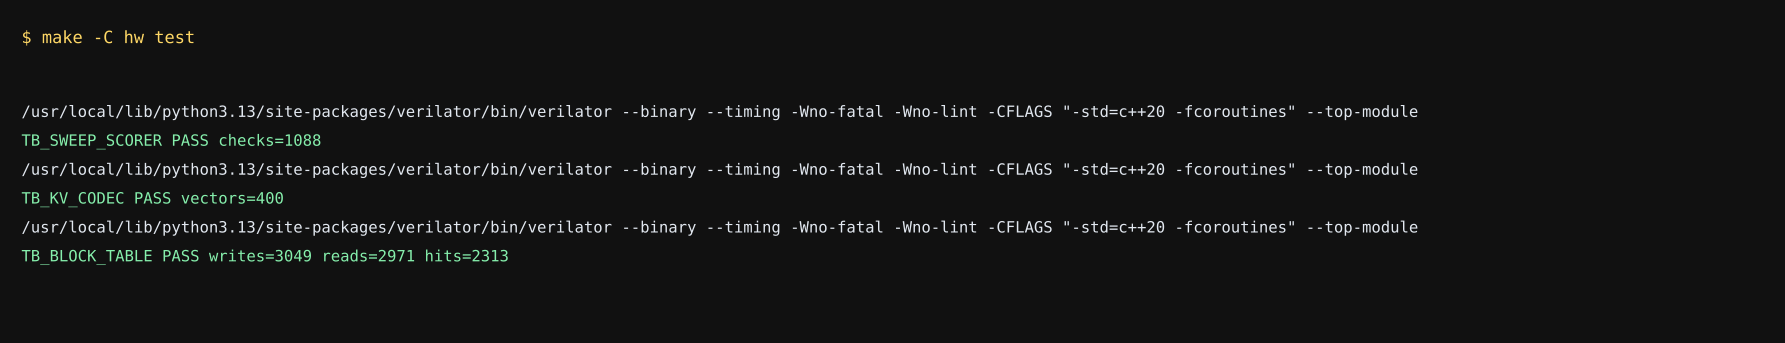
\includegraphics[width=6.27in,height=6.30in,keepaspectratio]{figs/t02_rtl_regression.png}}
\caption{Output of make -C hw test: all three testbenches print PASS with their check counts.}
\end{figure}
\begin{figure}[htbp]
\centering
\adjustbox{max width=\linewidth}{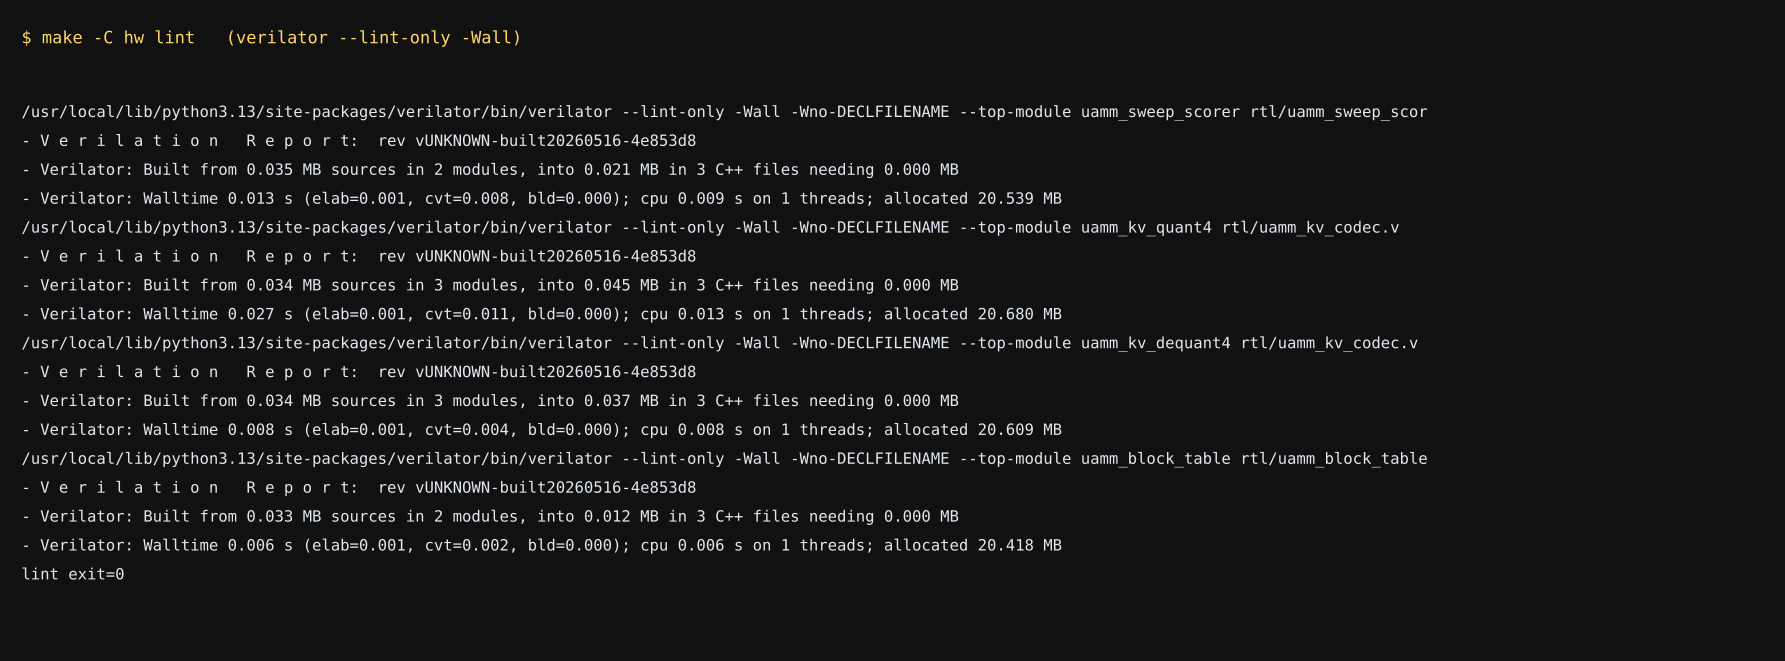
\includegraphics[width=6.27in,height=6.30in,keepaspectratio]{figs/t03_rtl_lint.png}}
\caption{Output of make -C hw lint (verilator --lint-only -Wall on every module). Exit status 0, no warnings.}
\end{figure}
\textbf{Mutation testing} measures the strength of the testbenches rather than the design: a testbench that cannot detect an injected fault is not protecting anything. Twelve mutants were generated, each a single small change to the RTL source, and the full regression was run on each.

\begin{figure}[htbp]
\centering
\adjustbox{max width=\linewidth}{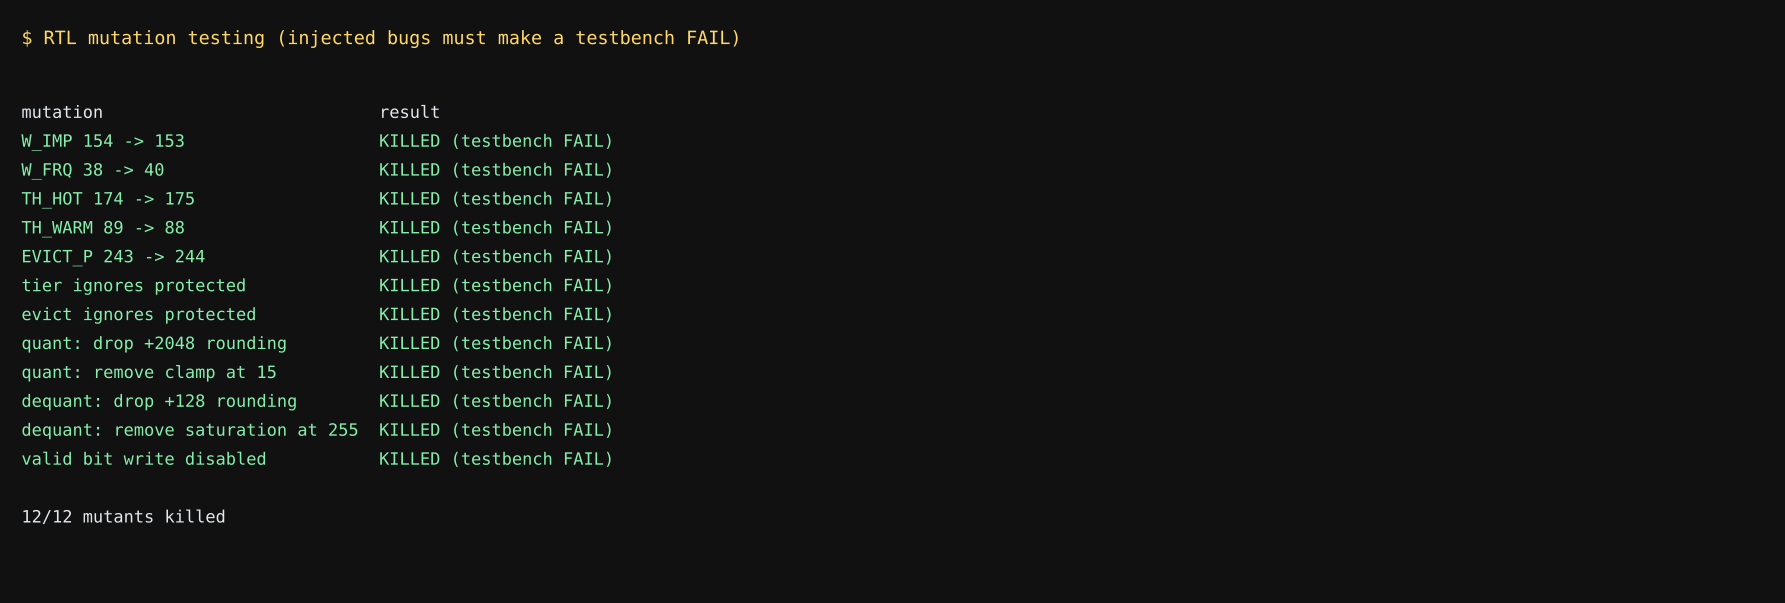
\includegraphics[width=6.27in,height=6.30in,keepaspectratio]{figs/t04_mutation.png}}
\caption{Mutation results: 12 of 12 injected faults are detected.}
\end{figure}
The mutants cover weights, thresholds, rounding, clamping, saturation, the protected-block override and the valid-bit write. During development one mutant (removing the clamp at code 15) initially \textbf{survived} because no vector exercised an out-of-range code; the stale-zero-point vectors described in Section~\ref{sec:9_3} were added to close that gap, and the mutant is now detected. This is the usual value of mutation testing\index{mutation testing}: it found a hole in the tests that a pass count alone would not have shown.

\subsection{Synthesis statistics}\label{sec:9_6}
{\fontsize{8}{9.5}\selectfont\setlength{\tabcolsep}{3pt}
\begin{longtable}{>{\raggedright\arraybackslash}p{1.70in}>{\raggedright\arraybackslash}p{0.85in}>{\raggedright\arraybackslash}p{0.85in}>{\raggedright\arraybackslash}p{0.93in}>{\raggedright\arraybackslash}p{0.68in}>{\raggedright\arraybackslash}p{0.68in}}
\caption{Yosys \texttt{synth -flatten} generic-cell statistics (technology-independent). The raw reports are in the repository under \texttt{docs/\allowbreak{}captures}.}\\
\toprule
\textbf{Module} & \textbf{Generic cells} & \textbf{Flip-flops} & \textbf{Combinational} & \textbf{Muxes} & \textbf{XOR/XNOR} \\\midrule\endfirsthead
\toprule \textbf{Module} & \textbf{Generic cells} & \textbf{Flip-flops} & \textbf{Combinational} & \textbf{Muxes} & \textbf{XOR/XNOR} \\\midrule\endhead
\bottomrule\endfoot
Sweep scorer (64 blocks) & 4,426 & 1,667 & 2,759 & 1,246 & 119 \\
Quantiser (16 lanes) & 11,292 & 65 & 11,227 & 4 & 3,252 \\
Dequantiser (16 lanes) & 5,241 & 129 & 5,112 & 0 & 1,364 \\
Block table (256 entries) & 12,796 & 4,370 & 8,426 & 3,155 & 8 \\
\bottomrule
\end{longtable}}
\begin{itemize}
\item The \textbf{block table\index{block table} and the scorer metadata} appear as thousands of flip-flops because the memories are written as generic arrays and Yosys\index{Yosys} was run without a memory-mapping step. On an FPGA or ASIC flow they would be mapped to block RAM or SRAM macros. The flip-flop counts are therefore an upper bound that reflects storage, not control logic.
\item The \textbf{quantiser is the largest logic block} (about 11,300 cells), dominated by the sixteen parallel 8 × 16-bit multipliers. A shift-based reciprocal (power-of-two ranges) or time-multiplexing fewer lanes would shrink it; this is noted as a design trade-off in Chapter~\ref{sec:12}.
\item These are technology-independent counts. \textbf{No place-and-route, timing or power analysis has been done.}
\end{itemize}
\section{The Ara Vector Kernel: Results}\label{sec:10}
The vector-processor part of the system is a C kernel (\texttt{ara/\allowbreak{}kv\_\allowbreak{}\allowbreak{}kernels.\allowbreak{}c}) that computes attention scores directly on 4-bit packed keys. It exists in two variants that share data layout and algorithm: a scalar path that executes on any host, and an RVV 1.0 path written with the standard vector intrinsics, compiled for a RISC-V\index{RISC-V} vector target.

\subsection{Algorithm in detail}\label{sec:10_1}
For a block of T tokens and d channels with per-channel scale s\_\allowbreak{}c and zero z\_\allowbreak{}c, the key of token t is reconstructed as k\_\allowbreak{}\{t,c\} = Q\_\allowbreak{}\{t,c\}·s\_\allowbreak{}c + z\_\allowbreak{}c. The attention logit is therefore:

\begin{center}\small\textit{q·k\_\allowbreak{}t = Σ\_\allowbreak{}c q\_\allowbreak{}c (Q\_\allowbreak{}\{t,c\} s\_\allowbreak{}c + z\_\allowbreak{}c) = Σ\_\allowbreak{}c (q\_\allowbreak{}c s\_\allowbreak{}c) Q\_\allowbreak{}\{t,c\} + Σ\_\allowbreak{}c q\_\allowbreak{}c z\_\allowbreak{}c = Σ\_\allowbreak{}c \textbackslash{}ensuremath\{\textbackslash{}tilde\{q\}\}\_\allowbreak{}c Q\_\allowbreak{}\{t,c\} + b}\end{center}
The pre-scaled query \textbackslash{}ensuremath\{\textbackslash{}tilde\{q\}\}\_\allowbreak{}c = q\_\allowbreak{}c·s\_\allowbreak{}c and the bias b = Σ q\_\allowbreak{}c z\_\allowbreak{}c are computed once per block (\texttt{kv\_\allowbreak{}\allowbreak{}qk\_\allowbreak{}\allowbreak{}prepare}), and \textbackslash{}ensuremath\{\textbackslash{}tilde\{q\}\} is de-interleaved into even-channel and odd-channel halves so that each packed byte (low nibble = even channel, high nibble = odd channel) multiplies two contiguous vectors. The per-token loop then does only integer-to-float conversion and fused multiply–add:

{\fontsize{8}{9.5}\selectfont\setlength{\tabcolsep}{3pt}
\begin{longtable}{>{\raggedright\arraybackslash}p{1.63in}>{\raggedright\arraybackslash}p{1.72in}>{\raggedright\arraybackslash}p{2.62in}}
\caption{Mapping from the scalar algorithm to the RVV instructions.}\\
\toprule
\textbf{Step per token} & \textbf{Scalar C} & \textbf{RVV instruction (observed in the compiled output)} \\\midrule\endfirsthead
\toprule \textbf{Step per token} & \textbf{Scalar C} & \textbf{RVV instruction (observed in the compiled output)} \\\midrule\endhead
\bottomrule\endfoot
Load packed bytes & \texttt{row[j]} & \texttt{vle8.\allowbreak{}v} (byte load with \texttt{vsetvli}) \\
Extract low / high nibble & \texttt{\& 0x0F}, \texttt{>> 4} & \texttt{vand.\allowbreak{}vx}, \texttt{vsrl.\allowbreak{}vi} \\
Widen to 32 bits & implicit & \texttt{vzext.\allowbreak{}vf4} \\
Convert to float & cast & \texttt{vfcvt.\allowbreak{}f.\allowbreak{}xu.\allowbreak{}v} \\
Load pre-scaled query halves & \texttt{qs\_\allowbreak{}\allowbreak{}even[j]}, \texttt{qs\_\allowbreak{}\allowbreak{}odd[j]} & \texttt{vle32.\allowbreak{}v} \\
Accumulate & \texttt{acc += …} & \texttt{vfmacc.\allowbreak{}vv} with tail-undisturbed policy \\
Reduce across lanes & sequential sum & \texttt{vfredusum.\allowbreak{}vs} \\
Add bias & \texttt{+ bias} & scalar add after \texttt{vfmv.\allowbreak{}f.\allowbreak{}s} \\
\bottomrule
\end{longtable}}
The tail-undisturbed (\texttt{\_\allowbreak{}\allowbreak{}tu}) form of the multiply–add matters for correctness: when the last strip of a row has fewer than a full vector of elements, the accumulator lanes beyond the active length must keep their previous values until the final reduction. Using the default tail-agnostic form could let those lanes be overwritten with arbitrary values.

\subsection{Numerical agreement (host)}\label{sec:10_2}
\begin{figure}[htbp]
\centering
\adjustbox{max width=\linewidth}{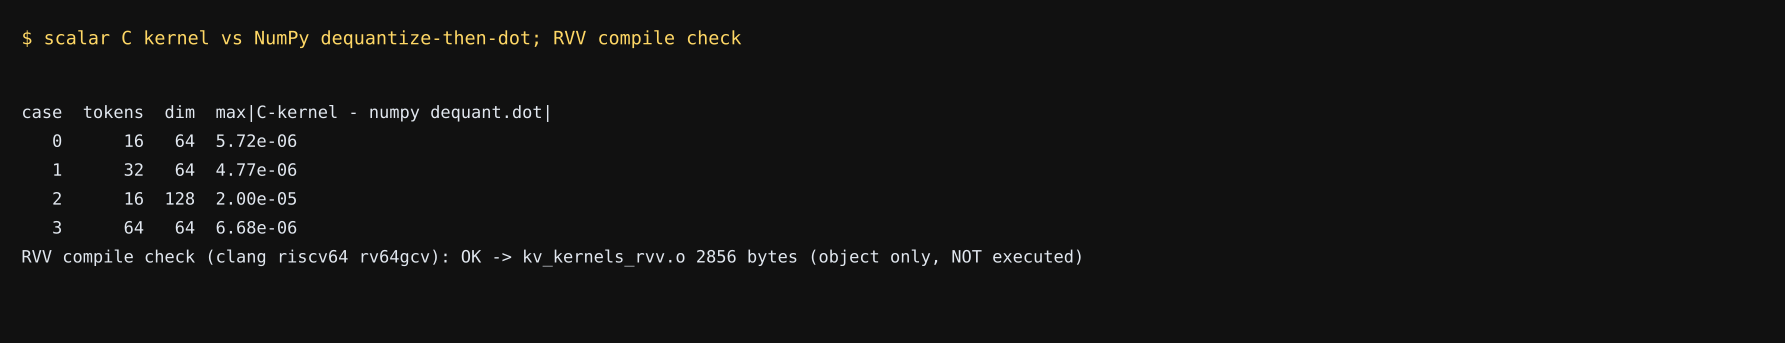
\includegraphics[width=6.27in,height=6.30in,keepaspectratio]{figs/t07_ara_check.png}}
\caption{Scalar C kernel versus NumPy dequantise-then-dot on random blocks, and the RVV compile check.}
\end{figure}
On four block shapes the maximum absolute difference between the C kernel and the straightforward NumPy computation (dequantise the whole block, then take the dot product) is between 4.8 × 10\textsuperscript{-}\textsuperscript{6} and 2.0 × 10\textsuperscript{-}\textsuperscript{5}, which is floating-point rounding for sums of 64–128 products of magnitude about one. The test suite also checks the pre-scaling algebra and the nibble order.

\subsection{RISC-V Vector compile check}\label{sec:10_3}
The same source was compiled with clang for \texttt{riscv64-unknown-elf} with \texttt{-march=rv64gcv -O2} (object file only). The inner loop of the compiled code is shown below; it contains the expected vector instructions listed in the mapping table above.

\begin{figure}[htbp]
\centering
\adjustbox{max width=\linewidth}{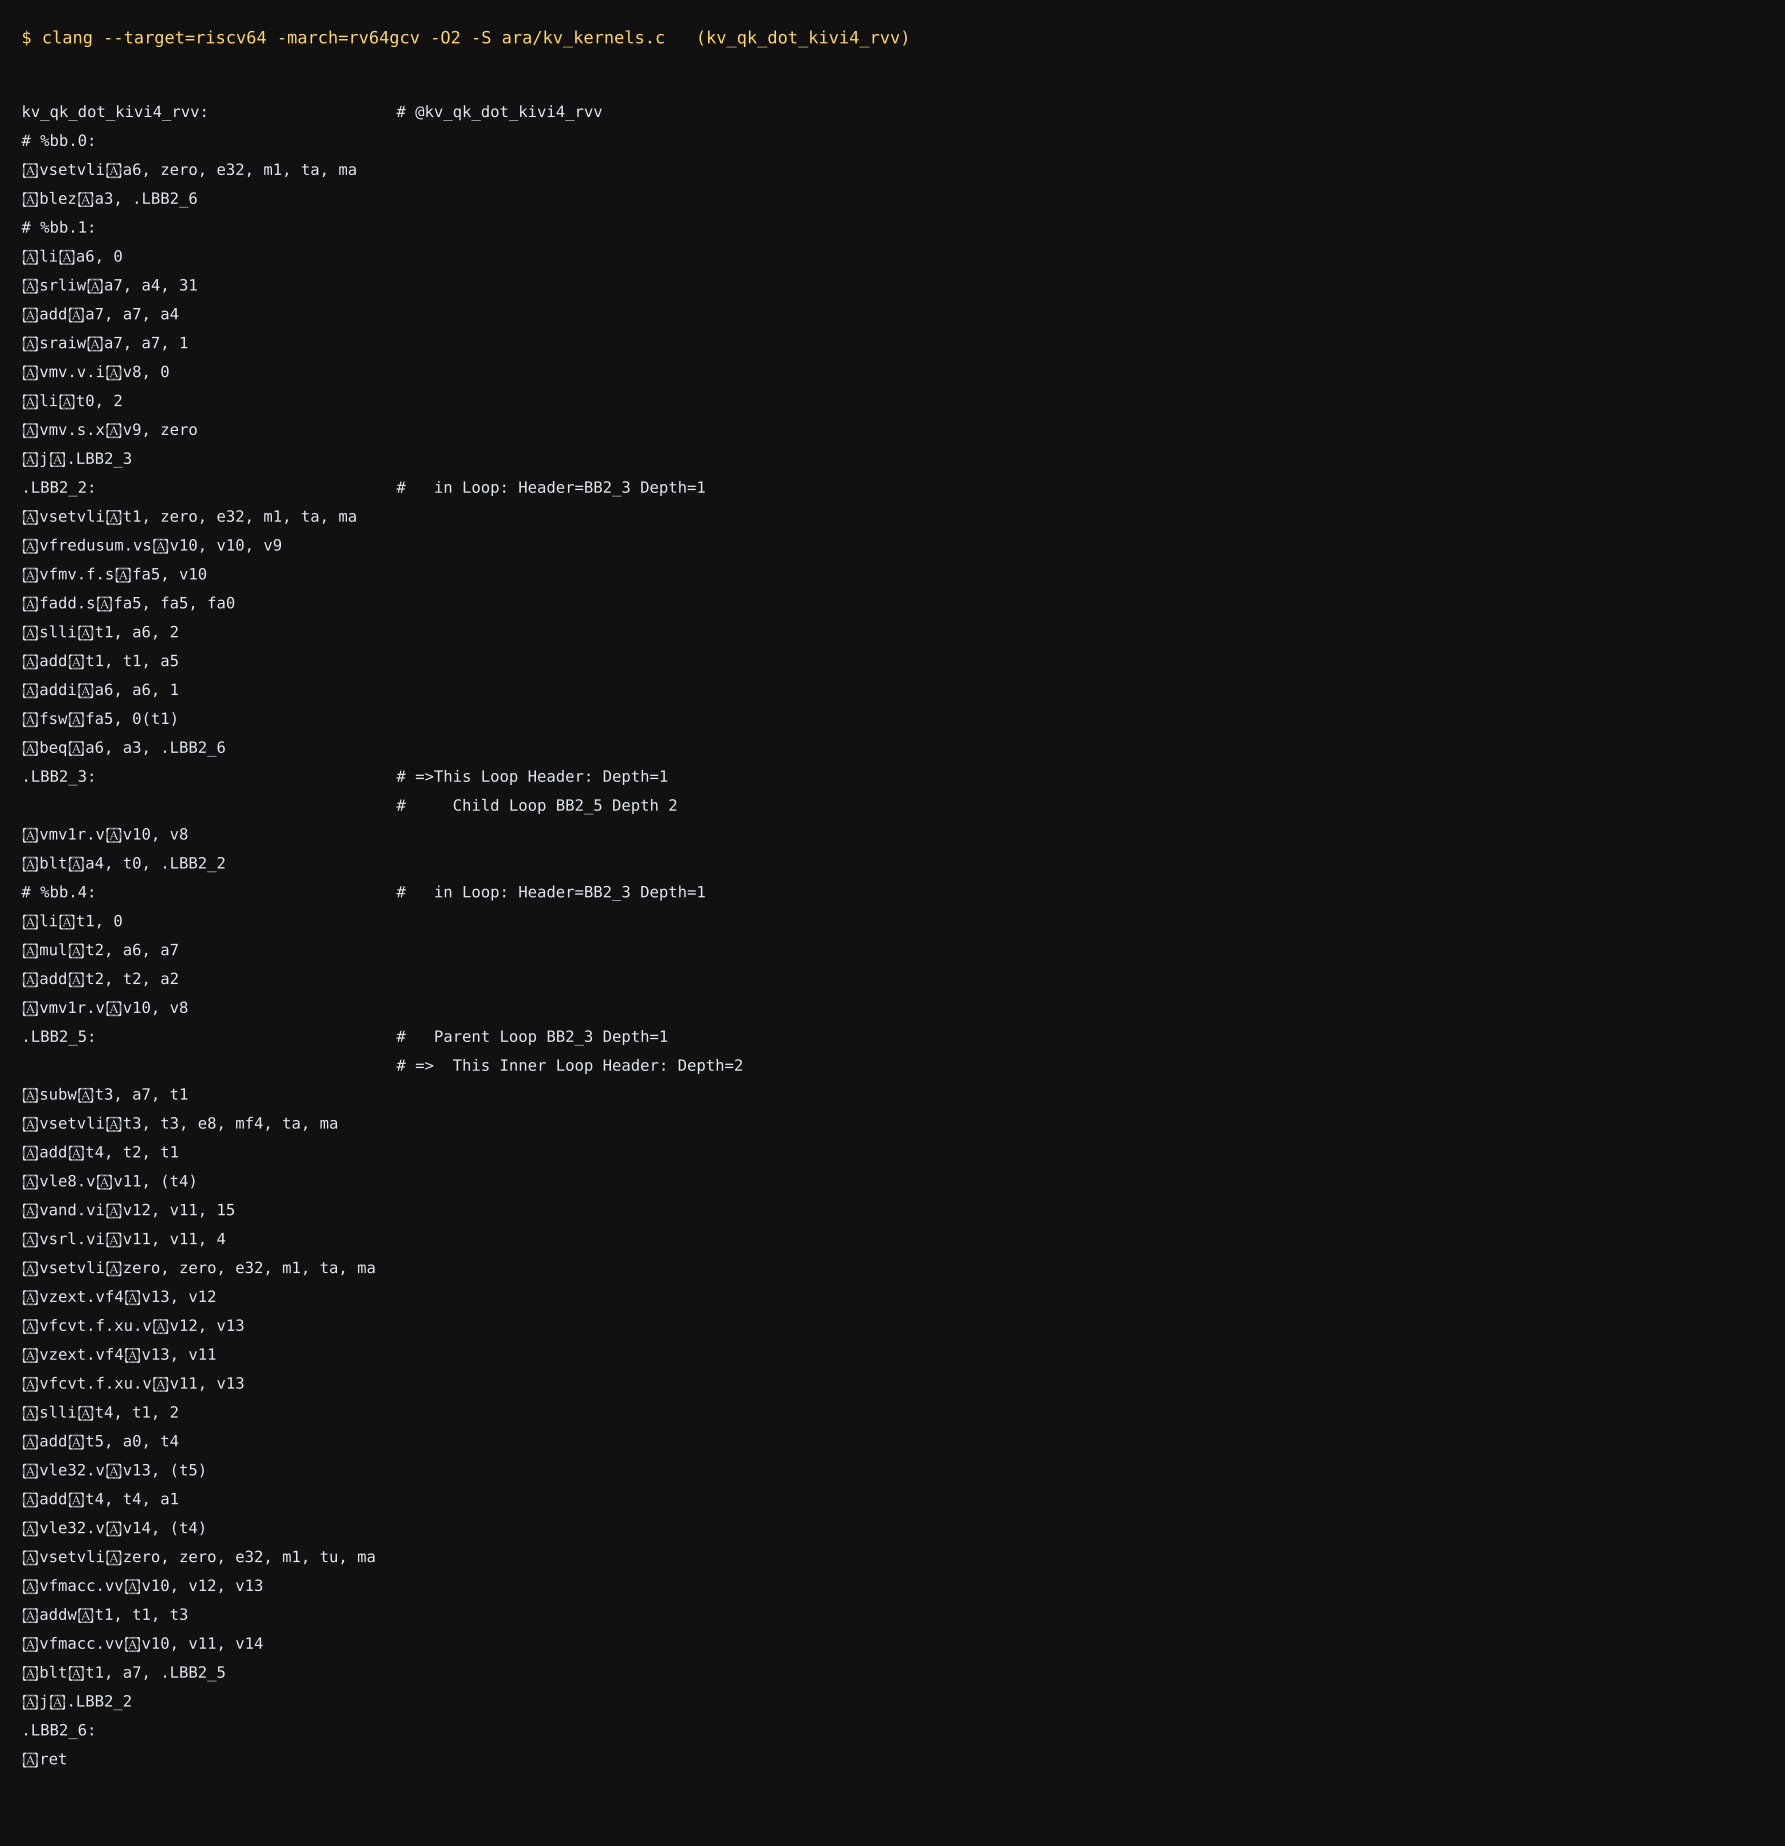
\includegraphics[width=6.27in,height=6.30in,keepaspectratio]{figs/t05_rvv_asm.png}}
\caption{RVV assembly for the 4-bit key kernel (excerpt of the compiler output).}
\end{figure}
This demonstrates that the intrinsics lower to the intended instruction sequence for a vector target. \textbf{It does not demonstrate that the code runs correctly or fast on Ara\index{Ara}:} no Ara, Spike or QEMU execution has been performed (Chapter~\ref{sec:12}).

\subsection{Why a fused kernel: bandwidth arithmetic}\label{sec:10_4}
An unfused implementation would first dequantise the key block into a floating-point buffer and then compute dot products. If that buffer is staged in memory, each 4-bit key element costs 0.5 bytes to read, 4 bytes to write and 4 bytes to read back (8.5 bytes of traffic) versus 0.5 bytes in the fused kernel, a factor of 17 in traffic for the key stream. If the dequantised tile is kept entirely in registers the memory traffic is the same as the fused kernel's but the kernel then executes the extra dequantisation instructions (a multiply and add per element) before each multiply–add. The fused form removes both. These are analytical counts from the algorithm, not measurements.

\begin{calloutbox}{What would make this a measured result}
Run the kernel on Spike for functional verification, then on the Ara\index{Ara} RTL simulation or an FPGA build to obtain cycles per token for block sizes of 16–64 tokens and head dimensions of 64–128; compare with a dequantise-then-dot baseline\index{baseline} written with the same intrinsics, on the same data.

\end{calloutbox}
\section{Scaling the Ratios to Larger Models: Arithmetic Only}\label{sec:13}
Section~\ref{sec:8} reports results on a small, deliberately tight configuration (168 KB for 1,536 tokens of a 64-channel cache). This chapter extrapolates those \textit{ratios} to the scale of an actual edge deployment, using arithmetic only. These are projections from measured ratios and stated assumptions, not new measurements.

\subsection{Why the compression ratios transfer to other geometries}\label{sec:13_1}
For a block of t tokens and d channels with value group g, the bytes of a b-bit block relative to FP16\index{FP16} are b/16 + 1/t + 1/g (scales and zeros are two FP16 numbers each, per channel for keys and per group for values). The expression does not depend on d. For t = 16 and g = 32 it gives 0.594 (INT8\index{INT8}), 0.344 (4-bit) and 0.219 (2-bit), identical to the measured values in Section~\ref{sec:5}. Larger blocks reduce the metadata share (t = 32 gives 0.3125 for 4-bit) but, as Section~\ref{sec:8_4_3} shows, enlarge the unit of placement.

\subsection{What fits on a phone-class device}\label{sec:13_2}
{\fontsize{8}{9.5}\selectfont\setlength{\tabcolsep}{3pt}
\begin{longtable}{>{\raggedright\arraybackslash}p{2.13in}>{\raggedright\arraybackslash}p{1.07in}>{\raggedright\arraybackslash}p{1.33in}>{\raggedright\arraybackslash}p{1.33in}}
\caption{Llama-3-8B-like geometry (131,072 B per token in FP16). The mixed rows use the resident ratios measured in E1 and assume the same mix at this scale.}\\
\toprule
\textbf{Storage} & \textbf{Bytes vs FP16} & \textbf{Max tokens in 1 GiB} & \textbf{KV size at 32K tokens} \\\midrule\endfirsthead
\toprule \textbf{Storage} & \textbf{Bytes vs FP16} & \textbf{Max tokens in 1 GiB} & \textbf{KV size at 32K tokens} \\\midrule\endhead
\bottomrule\endfoot
FP16 & 1.000 & 8,192 & 4.00 GiB \\
INT8 & 0.594 & 13,791 & 2.38 GiB \\
Mixed int8/4-bit (E1: 0.371) & 0.371 & 22,081 & 1.48 GiB \\
Mixed incl. 2-bit (E1: 0.310) & 0.310 & 26,426 & 1.24 GiB \\
All 4-bit & 0.344 & 23,814 & 1.38 GiB \\
All 2-bit & 0.219 & 37,406 & 0.88 GiB \\
\bottomrule
\end{longtable}}
In the model, a 1 GiB KV budget\index{budget} that holds about 8,200 tokens in FP16\index{FP16} holds about 26,000 tokens at the 0.310 mix without dropping any: a gain of 3.2×, in line with 1/0.310. A 32K-token context shrinks from 4 GiB to about 1.2 GiB.

\subsection{Reads per token}\label{sec:13_3}
In the 1,536-token run, after step 1,024 the engine read on average 35 \% of the blocks per decode step (24 selected plus the protected set). If the same fraction applied at larger scale and the blocks read had the average encoding, bytes read per token would be roughly 0.35 × 0.31 = 0.11 of the dense FP16\index{FP16} read. The fraction would shrink further with longer contexts because the block budget\index{budget} is fixed while the cache grows, but recall\index{recall} would also fall (Section~\ref{sec:8_3}); the budget has to be tuned against the application's quality needs.

{\fontsize{8}{9.5}\selectfont\setlength{\tabcolsep}{3pt}
\begin{longtable}{>{\raggedright\arraybackslash}p{0.78in}>{\raggedright\arraybackslash}p{1.21in}>{\raggedright\arraybackslash}p{1.38in}>{\raggedright\arraybackslash}p{1.38in}>{\raggedright\arraybackslash}p{1.03in}}
\caption{Projected KV-read bound for the 8B-like geometry. For 8,192 tokens the measured read fraction is used; beyond that the fixed 24-block budget plus a 36-token protected set is assumed. Weight reads and compute are ignored, and the bound is not a prediction of end-to-end speed.}\\
\toprule
\textbf{Context} & \textbf{Dense FP16 KV read / token} & \textbf{KV-only bound (tok/s, 12.8 GB/s)} & \textbf{Selective + mixed codecs read / token} & \textbf{KV-only bound (tok/s)} \\\midrule\endfirsthead
\toprule \textbf{Context} & \textbf{Dense FP16 KV read / token} & \textbf{KV-only bound (tok/s, 12.8 GB/s)} & \textbf{Selective + mixed codecs read / token} & \textbf{KV-only bound (tok/s)} \\\midrule\endhead
\bottomrule\endfoot
8,192 & 1.00 GiB & 11.9 & 112 MiB & 109.3 \\
32,768 & 4.00 GiB & 3.0 & 16 MiB & 750.0 \\
131,072 & 16.00 GiB & 0.7 & 16 MiB & 750.0 \\
\bottomrule
\end{longtable}}
These bounds extrapolate from one 64-channel head on synthetic data and from a read fraction measured at 1,536 tokens. They illustrate the arithmetic; no model of this size was run and they are not predictions of speed. At 32K tokens the dense FP16\index{FP16} read bound is about 3 tokens per second on 12.8 GB/s memory; with selective reads and mixed codecs the KV-only bound is far higher, which would make the weights, not the cache, the limit again. This is the sense in which the design aims to restore the bottleneck to where it belongs. Whether recall\index{recall} at 24 blocks is sufficient at that length for a real model is exactly the question that real-model validation (Chapter~\ref{sec:12}, gap 1) must answer.

\subsection{What would convince a sceptic}\label{sec:13_4}
{\fontsize{8}{9.5}\selectfont\setlength{\tabcolsep}{3pt}
\begin{longtable}{>{\raggedright\arraybackslash}p{1.99in}>{\raggedright\arraybackslash}p{1.99in}>{\raggedright\arraybackslash}p{1.99in}}
\caption{Evidence available and evidence needed for each claim.}\\
\toprule
\textbf{Claim} & \textbf{Evidence in this report} & \textbf{Evidence still needed} \\\midrule\endfirsthead
\toprule \textbf{Claim} & \textbf{Evidence in this report} & \textbf{Evidence still needed} \\\midrule\endhead
\bottomrule\endfoot
The joint policy beats placement alone in a tight budget & E1, E2, E5 on the synthetic trace (a one-codec 4-bit baseline matches its feasibility, E1 and E10) & Same ablation on real traces, with task accuracy \\
Hysteresis and cadence control churn & E4 & Energy measured on a device \\
Hardware blocks implement the specified arithmetic & Bit-exact RTL regression, mutation tests, lint & Place-and-route, timing, power, integration with a bus \\
The kernel is correct & Host agreement with NumPy; RVV compiles & Execution on Spike/Ara \\
The design speeds up an edge device & Modelled fetch time (in the model the planner is slower than a one-codec 4-bit baseline) & Measured tokens/s on target hardware \\
\bottomrule
\end{longtable}}
\section{Conclusions we can draw}
\begin{itemize}
\item \textbf{Choosing precision together with placement fixes the capacity problem.} With a budget\index{budget} smaller than the FP16\index{FP16} data, UAMM-1\index{UAMM-1} had to delete 63 \% of the tokens. UAMM-2\index{UAMM-2} kept all of them at a measured error.
\item \textbf{The codecs do most of that work.} A single 4-bit codec\index{codec} for every block also fits. The planner\index{planner} is not what makes the data fit.
\item \textbf{The planner buys accuracy and robustness.} At the same size it has lower error than the 4-bit baseline\index{baseline}, with 2-bit blocks it gets smaller, and it still fits when the budget\index{budget} is tightened.
\item \textbf{Reading less matters as much as storing less.} Reading 24 of about 96 blocks keeps 94.5 \% of the attention mass.
\item \textbf{Stability needs explicit rules.} Hysteresis, a minimum residency\index{residency} and a replanning interval reduced migrations from 1,871 to 630.
\item \textbf{Small hardware blocks can be verified thoroughly.} The three RTL modules are bit-exact against their models, and 12 of 12 injected bugs were caught. The scorer implements UAMM-1\index{UAMM-1}'s score, not the planner\index{planner}'s cost.
\end{itemize}
\section{Did we do anything new?}
Almost every ingredient of UAMM-2\index{UAMM-2} comes from a published method, and we have said so wherever it appears. We do not claim a new algorithm for any one of them. What we think is new, or at least not something we found in the papers we read, is the following combination and the way it was checked.

\begin{itemize}
\item Treating a block's placement as a (tier\index{tier}, codec\index{codec}) pair and choosing it with one cost that adds read time, decode time, a measured quantisation\index{quantisation} penalty weighted by heat, and a capacity price, under per-tier byte limits.
\item A precision ratchet\index{precision ratchet} and an opt-in drop, so that every loss in quality is explicit and capacity overflow is reported as a number and never hidden.
\item Using Quest\index{Quest}-style min/max bounds to choose the blocks to read in a system whose blocks are stored at different precisions in different tiers.
\item A small hardware path (scorer, 4-bit quantiser and dequantiser without a divider, block table\index{block table}) checked against bit-exact models and by mutation testing\index{mutation testing}, together with a fused vector kernel that works on packed 4-bit keys.
\item A measurement habit that we consider part of the contribution: a fair one-codec baseline\index{baseline}, a capacity-aware version of UAMM-1\index{UAMM-1}, charging the metadata to the budget\index{budget}, and a budget sweep that shows where the advantage disappears.
\end{itemize}
What we do not claim: a speed-up on real hardware, results on real language models, or any result from running on Ara\index{Ara}. Those require measurements we have not made.

\chapter{Future Scope}\label{sec:12}
UAMM-2\index{UAMM-2} is a first complete version, not a finished system. While building it and reading the results we kept running into places where the design could be taken further. This chapter collects them as research scopes. For each one we describe what UAMM-2 does today, what we noticed, how we think it could be improved and how we would go about building and testing it. None of this is implemented or tested yet. These are directions we think are worth following, and the sketches show where a change would go in the code.

\begin{calloutbox}{Status of this chapter}
Everything here is future work. No scope in this chapter has been implemented or measured. Where we quote a number, it is a result from the simulations in Section~\ref{sec:8} that motivated the idea.

\end{calloutbox}
\section{Scopes on precision}
\subsection{Scope 1: Different bit widths for keys and for values}
\textbf{Where UAMM-2 is today.} Keys and values of a block use the same bit width, whatever codec\index{codec} the planner\index{planner} picks.

\textbf{What we noticed.} The two enter attention in different ways. An error in a key changes a logit, and the softmax then scales that token's weight by about e to the power of the change, so a small key error can reorder tokens whose logits are close. An error in a value only shifts the output linearly. In our workload the 2-bit codec\index{codec} has a squared error of 0.130 per block. That looks tolerable for values but risky for keys.

\textbf{How we could take it forward.} We may separate the two widths and let the planner\index{planner} choose a pair such as K4/V2, so that keys keep more bits than values. The planner would price the two error terms separately, since the two do not hurt attention equally.

\textbf{How we would build it.} The codec\index{codec} name would carry two widths, \texttt{encode} would take \texttt{bits\_\allowbreak{}\allowbreak{}k} and \texttt{bits\_\allowbreak{}\allowbreak{}v}, and calibration would measure a logit error for keys (the largest |q·(k − \textbackslash{}ensuremath\{\textbackslash{}hat\{k\}\})| over sampled queries) next to the value error. We would test it by comparing K4/V2 with 3-bit for both at the same memory.

\begin{lstlisting}
# codecs.py (sketch)
def encode(k, v, bits_k, bits_v, v_group):
    qk, sk, zk = _asym_quant(k, bits_k, axis=0)          # per-channel keys
    qv, sv, zv = _asym_quant(v_grouped, bits_v, axis=2)   # per-token values
    return pack(qk, bits_k) + pack(qv, bits_v) + meta

# planner cost with separate quality terms
cost = p*read_ms + lam_k*heat*err_logit_k[c] + lam_v*heat*err_v[c] + congestion
\end{lstlisting}
\subsection{Scope 2: Knowing when a compressed block is safe to use}
\textbf{Where UAMM-2 is today.} The planner\index{planner} uses an average error measured when the block is sealed. It does not know whether, for the current query, a compressed block could change which tokens rank highest.

\textbf{What we noticed.} With a per-channel scale s\_\allowbreak{}c, the dequantisation error in channel c is at most s\_\allowbreak{}c/2, so for a query q the logit error of any token in the block is bounded by ½ Σ|q\_\allowbreak{}c|·s\_\allowbreak{}c. That is one dot product with the scale vector, and the selection step already does something very similar with the min/max summaries.

\textbf{How we could take it forward.} At selection time we could compute this bound for every candidate block. If it is large compared with the logit gap to the next block in the ranking, the block is risky and we would read it from a higher-precision copy or keep it out of the approximate path.

\textbf{How we would build it.} The per-channel key scales are already in each payload. We would keep them as a small resident vector, add an \texttt{err\_\allowbreak{}\allowbreak{}bound(q, block)} function next to \texttt{select\_\allowbreak{}\allowbreak{}blocks}, and measure how often it flags a block whose error actually changed the output.

\begin{lstlisting}
def err_bound(q, scale_k):          # per-channel key scales of the block
    return 0.5 * float(np.abs(q) @ scale_k)

risky = [b for b in chosen if err_bound(q, b.scale_k) > tau]
\end{lstlisting}
\subsection{Scope 3: Better quantisation ranges: outlier tokens and clipping}
\textbf{Where UAMM-2 is today.} Keys are scaled per channel, which deals with channels that are large for every token. The range of a block is its exact minimum and maximum.

\textbf{What we noticed.} A single token with an unusually large key stretches the range of every channel it touches, and the other 15 tokens then use only a few levels. Heavy-hitter and sink tokens are the ones most likely to be large and the ones we most want to keep accurate. Our block-size sweep points the same way: 8-token blocks had the lowest error (0.110) and 64-token blocks the highest (0.341).

\textbf{How we could take it forward.} Two ideas fit together. One is a small FP16\index{FP16} side buffer for the largest one or two tokens of a block, left out of the range calculation. The other is to take the range from the 2nd and 98th percentile of each channel and let the side buffer hold what is clipped. Calibration already encodes each block once, so trying a second clipping level costs one more encode.

\textbf{How we would build it.} In \texttt{\_\allowbreak{}\allowbreak{}asym\_\allowbreak{}\allowbreak{}quant} we would find the rows with the largest key norm, replace them by the channel median before computing min and max, and append (index, key, value) records to the payload. The overhead is 256 bytes per block for one outlier at 64 channels. We would test on data with injected outlier tokens.

\begin{lstlisting}
idx = np.argsort(-np.linalg.norm(k, axis=1))[:m]
k_clip = k.copy(); k_clip[idx] = np.median(k, axis=0)
q, s, z = _asym_quant(k_clip, bits, axis=0)
payload += pack_sidecar(idx, k[idx], v[idx])   # exact rows
\end{lstlisting}
\subsection{Scope 4: Keeping track of error across repeated re-encoding}
\textbf{Where UAMM-2 is today.} Each block carries an error table measured against its FP16\index{FP16} original when it is sealed. Re-encoding decodes the current payload and encodes it again.

\textbf{What we noticed.} A block that goes from INT8\index{INT8} to 4-bit to 2-bit ends up with more error than the 2-bit entry of its table says, so the planner\index{planner} underestimates the cost of its own earlier decisions. If the errors are independent, the total is roughly 1 − (1 − e\textsubscript{1})(1 − e\textsubscript{2}).

\textbf{How we could take it forward.} We could keep an accumulated error per block, use it in the quality term and in the ratchet check, and limit the number of lossy steps. For cold blocks a copy of the FP16\index{FP16} original could stay in flash\index{flash} so that re-encoding always starts from it.

\textbf{How we would build it.} We would add an \texttt{err\_\allowbreak{}\allowbreak{}acc} field to the block, update it in \texttt{reencode}, and have the planner\index{planner} use the larger of the table value and the accumulated value. The test is to compare the predicted error of long-lived blocks with the error measured after the fact.

\begin{lstlisting}
b.err_acc = 1 - (1 - b.err_acc) * (1 - b.err_table[codec])      # in reencode()
\end{lstlisting}
\subsection{Scope 5: Choosing precision by sensitivity, and keeping a quality floor}
\textbf{Where UAMM-2 is today.} The planner\index{planner} lowers precision according to how hot a block is, and the cost function trades accuracy for speed everywhere, even when memory is plentiful.

\textbf{What we noticed.} Two blocks with the same heat can differ in how much their error moves the output, because it also depends on the size of their values and on how sharp the logits are. We also saw that spare memory is not always put to good use. At 512 tokens the cache fits in FP16\index{FP16} with error 0.0013 under UAMM-1\index{UAMM-1}, but UAMM-2\index{UAMM-2} still compresses it and the error becomes 0.016.

\textbf{How we could take it forward.} We may replace heat by a sensitivity score (mean attention weight times a measure of how much the block's error can change the output) and only demote a block when its tier\index{tier} is under pressure. A per-request error budget\index{budget} would let the user say how much total error is acceptable, with the planner\index{planner} refusing a demotion that would break it.

\textbf{How we would build it.} \texttt{h2o.\allowbreak{}py} already provides the mean attention weight, and sealing could store the norm of the values. We would add a fill threshold to \texttt{Config}, a \texttt{pressure(tier)} function to \texttt{tiers.\allowbreak{}py} and a running error sum to the planner\index{planner}. We would check that error no longer rises when the budget\index{budget} is increased.

\begin{lstlisting}
if used[t] / cap[t] < cfg.min_fill_to_demote and codec_rank(c) > b.rank:
    continue                                   # no pressure: keep precision
if err_sum + heat * new_err > cfg.error_budget:
    continue
\end{lstlisting}
\subsection{Scope 6: Storing keys before positional encoding}
\textbf{Where UAMM-2 is today.} The engine stores whatever key vector it is given. In a real model that vector has usually been through rotary position embedding (RoPE).

\textbf{What we noticed.} The rotation changes the per-channel statistics with position and mixes large channels into their partners, which weakens per-channel quantisation\index{quantisation}.

\textbf{How we could take it forward.} We could store keys before the rotation and apply it on the query side instead, because (R\_\allowbreak{}p k)·q equals k·(R\_\allowbreak{}p\textsuperscript{T} q). For a block of 16 tokens that is 16 rotated copies of the query, which is small next to reading the keys.

\textbf{How we would build it.} The kernel call would take cosine and sine tables for the positions of the block. We would test it on a real model's keys, which we do not have yet.

\section{Scopes on placement and policy}
\subsection{Scope 7: Prefetching blocks before they are needed}
\textbf{Where UAMM-2 is today.} A block is fetched when attention asks for it. If the query returns to an old topic, the first reads wait for flash\index{flash}.

\textbf{What we noticed.} Replanning every 64 steps gave 3,326 flash\index{flash} reads and 0.272 ms per token, against 599 reads and 0.090 ms with replanning every 2 steps. Replanning often costs migrations (768 against 345), so there is a trade-off we cannot fix by only changing the interval.

\textbf{How we could take it forward.} Selection already ranks every block. The blocks ranked just below the ones we read are the most likely to be read next, so we could promote those that sit in flash\index{flash} into DRAM while the current attention step is running.

\textbf{How we would build it.} A \texttt{prefetch(q, candidates)} function in \texttt{attention.\allowbreak{}py} would return block ids. The simulator would move them through the runtime adapter with a cost charged to a background channel. We would measure flash\index{flash} reads and time per token against the numbers above.

\begin{lstlisting}
ranked = np.argsort(-bound)
read     = ranked[:B]
prefetch = [b for b in ranked[B:B+P] if tier[b] == FLASH]   # promote ahead of need
\end{lstlisting}
\subsection{Scope 8: Layers, heads and grouped-query attention}
\textbf{Where UAMM-2 is today.} The engine keeps one flattened vector per token, which is one head of one layer in effect.

\textbf{What we noticed.} A model of the 8B class has 32 layers with 8 KV heads each, which is 256 separate streams with different attention patterns. One global budget\index{budget} of 24 blocks would starve heads that look broadly and waste reads on heads that look sharply.

\textbf{How we could take it forward.} We would add the layer and head to the identity of a block and give each stream its own read budget\index{budget} in proportion to the entropy of its attention, as PyramidKV and FastGen do in their own ways.

\textbf{How we would build it.} The block would gain \texttt{layer} and \texttt{head} fields, the importance tracker would keep one score array per stream, and the block table\index{block table} in the RTL would need a few more address bits. This is the largest change on our list, since it touches almost every module.

\subsection{Scope 9: A better optimiser than the greedy planner}
\textbf{Where UAMM-2 is today.} The planner\index{planner} visits blocks from hottest to coldest and each takes its cheapest feasible slot.

\textbf{What we noticed.} In the budget\index{budget} sweep the error was 0.115 at twice the budget but 0.152 at three times, which means the heuristic is not always close to a good assignment.

\textbf{How we could take it forward.} We may write the choice as a multiple-choice knapsack, solve it offline on recorded traces to see how far the greedy answer is from the best one, and, if the gap matters, use a price per tier\index{tier} that is adjusted until the capacities are met. That maps onto the congestion term the planner\index{planner} already has, and FlexGen formulates placement in a similar way.

\textbf{How we would build it.} The offline solver only needs the cost table of each block. The online version is a short dual-update loop.

\begin{lstlisting}
for it in range(20):
    choice = {b: argmin_tc(cost(b,t,c) + price[t]*bytes(b,c)) for b in blocks}
    for t in tiers:
        price[t] = max(0, price[t] + step * (used(choice,t) - cap[t]))
\end{lstlisting}
\subsection{Scope 10: Counting and shrinking the selection summaries}
\textbf{Where UAMM-2 is today.} Each block keeps minimum and maximum key vectors in FP16\index{FP16} so that attention can choose blocks. The main experiments do not count them against the memory budget\index{budget}.

\textbf{What we noticed.} They take 256 bytes per block at 64 channels, which is 14 \% of our 168 KB budget\index{budget}. When we charged them in the key-summary experiment, some variants stopped fitting.

\textbf{How we could take it forward.} We could store the summaries in 8 bits (rounding the minimum down and the maximum up so the bound stays valid), or keep one summary for each group of eight channels and accept a looser bound.

\textbf{How we would build it.} The summary arrays would become \texttt{int8}. We would measure how much the selection recall\index{recall} changes, since a looser bound makes the selection less sharp.

\subsection{Scope 11: When the budget runs out, and sharing between sequences}
\textbf{Where UAMM-2 is today.} If even 2-bit blocks do not fit, the planner\index{planner} reports the overflow and stops. Each sequence also owns all of its blocks.

\textbf{What we noticed.} At 3,072 tokens the all-codec system overflows by 28.5 KB. A system prompt of 800 tokens shared by four sessions takes four times the memory of one copy.

\textbf{How we could take it forward.} As a last resort we could drop the least important tokens inside the least important blocks, at token level and with an explicit counter. For shared prompts we could count references to blocks and copy a block only when someone writes to it, the way PagedAttention\index{PagedAttention} does.

\textbf{How we would build it.} A \texttt{compact(block, keep\_\allowbreak{}\allowbreak{}mask)} function would re-encode a block with fewer tokens and \texttt{allow\_\allowbreak{}\allowbreak{}drop} would become never, block or token. Sharing needs a reference count in the block and a table from the hash of the prefix to a block.

\section{Scopes on systems and hardware}
\subsection{Scope 12: Moving blocks safely while attention is running, and flash wear}
\textbf{Where UAMM-2 is today.} In the simulator a block moves instantly. Every demotion into flash\index{flash} is also treated like any other move.

\textbf{What we noticed.} On a real system a block may be re-encoded while a step is reading it, which would mix two formats in one result. Flash also has limited write endurance, and the planner\index{planner} can still move a block back and forth between DRAM and flash\index{flash}.

\textbf{How we could take it forward.} We could give every block-table entry a version number, write the new payload to a second buffer and then switch the entry in one update. A step that sees the version change would read again. For flash\index{flash} we could count writes, add their cost to the move cost and ask for a larger improvement before a block is moved into flash.

\textbf{How we would build it.} The block-table RTL already returns the old entry when a read and a write collide, so it is a natural place for the version number. The wear counters live in \texttt{tiers.\allowbreak{}py}.

\subsection{Scope 13: Bringing the hardware closer to the planner}
\textbf{Where UAMM-2 is today.} The Verilog scorer computes the original UAMM-1\index{UAMM-1} weighted score, not the planner\index{planner}'s utility cost, and the codec\index{codec} works on 8-bit data while the software codecs start from FP16\index{FP16}. Nothing has been placed and routed.

\textbf{What we noticed.} The quantiser alone is about 11,300 generic gates, mostly sixteen 8 × 16-bit multipliers.

\textbf{How we could take it forward.} We would add a front stage that turns FP16\index{FP16} into a group-normalised 8-bit value using the group minimum and maximum from firmware. We would write the utility cost in fixed point with small lookup tables for the read-time and error terms. We could also save area by rounding the range up to a power of two, so the reciprocal multiplier becomes a shift, or by using fewer lanes.

\textbf{How we would build it.} The new scorer would be checked the same way as the current one: a bit-exact model, boundary vectors and a mutation test. Place and route would be the first step towards real area and timing numbers.

\section{Order of work}
If we were to carry on, we would start with the scopes that need no new data and finish with those that need a real model or real hardware.

{\fontsize{8}{9.5}\selectfont\setlength{\tabcolsep}{3pt}
\begin{longtable}{>{\raggedright\arraybackslash}p{0.53in}>{\raggedright\arraybackslash}p{3.92in}>{\raggedright\arraybackslash}p{1.51in}}
\caption{Suggested order of work.}\\
\toprule
\textbf{Step} & \textbf{Goal} & \textbf{Scopes} \\\midrule\endfirsthead
\toprule \textbf{Step} & \textbf{Goal} & \textbf{Scopes} \\\midrule\endhead
\bottomrule\endfoot
1 & Precision control: separate key and value widths, error bound, outliers and clipping, error tracking, sensitivity & 1, 2, 3, 4, 5, 6 \\
2 & Policy: prefetch, layers and heads, a better optimiser, counting summaries & 7, 8, 9, 10 \\
3 & Limits and sharing: token-level fallback, copy-on-write & 11 \\
4 & Systems and hardware: safe migration, flash wear, utility scorer in RTL & 12, 13 \\
\bottomrule
\end{longtable}}
\chapter{Project Timeline}
The work ran from 10 August 2026 to the middle of November 2026. The first draft was submitted on 24 August, and everything after that is the work reported here. Dates after the first draft are approximate periods, since several activities overlapped.

\begin{figure}[htbp]
\centering
\adjustbox{max width=\linewidth}{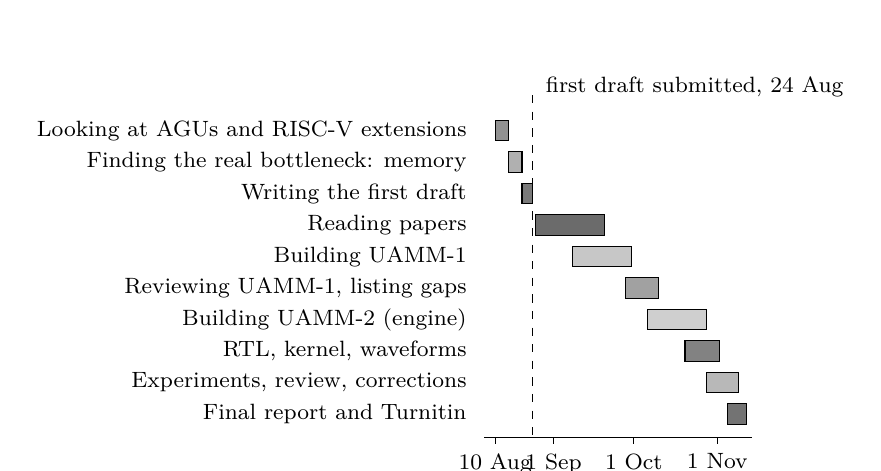
\begin{tikzpicture}[font=\footnotesize]
\node[anchor=east] at (2.65,-0.00) {Looking at AGUs and RISC-V extensions};
\draw[fill=black!43] (2.89,-0.13) rectangle (3.06,0.13);
\node[anchor=east] at (2.65,-0.40) {Finding the real bottleneck: memory};
\draw[fill=black!31] (3.06,-0.53) rectangle (3.23,-0.27);
\node[anchor=east] at (2.65,-0.80) {Writing the first draft};
\draw[fill=black!52] (3.23,-0.93) rectangle (3.36,-0.67);
\node[anchor=east] at (2.65,-1.20) {Reading papers};
\draw[fill=black!58] (3.40,-1.33) rectangle (4.28,-1.07);
\node[anchor=east] at (2.65,-1.60) {Building UAMM-1};
\draw[fill=black!22] (3.87,-1.73) rectangle (4.62,-1.47);
\node[anchor=east] at (2.65,-2.00) {Reviewing UAMM-1, listing gaps};
\draw[fill=black!37] (4.55,-2.13) rectangle (4.96,-1.87);
\node[anchor=east] at (2.65,-2.40) {Building UAMM-2 (engine)};
\draw[fill=black!19] (4.82,-2.53) rectangle (5.57,-2.27);
\node[anchor=east] at (2.65,-2.80) {RTL, kernel, waveforms};
\draw[fill=black!49] (5.30,-2.93) rectangle (5.74,-2.67);
\node[anchor=east] at (2.65,-3.20) {Experiments, review, corrections};
\draw[fill=black!28] (5.57,-3.33) rectangle (5.98,-3.07);
\node[anchor=east] at (2.65,-3.60) {Final report and Turnitin};
\draw[fill=black!55] (5.84,-3.73) rectangle (6.08,-3.47);
\draw (2.75,-3.90) -- (6.15,-3.90);
\draw (2.89,-3.90) -- ++(0,-0.08) node[below] {10 Aug};
\draw (3.63,-3.90) -- ++(0,-0.08) node[below] {1 Sep};
\draw (4.65,-3.90) -- ++(0,-0.08) node[below] {1 Oct};
\draw (5.71,-3.90) -- ++(0,-0.08) node[below] {1 Nov};
\draw[dashed] (3.36,0.45) -- (3.36,-3.90); \node[anchor=west] at (3.41,0.55) {first draft submitted, 24 Aug};
\end{tikzpicture}}
\caption{Project timeline. Bars show the approximate period of each activity.}
\end{figure}
\section{From 10 to 24 August: finding the problem}
{\fontsize{9}{10.5}\selectfont\setlength{\tabcolsep}{3pt}
\begin{longtable}{>{\raggedright\arraybackslash}p{0.95in}>{\raggedright\arraybackslash}p{5.11in}}
\caption{The first two weeks.}\\
\toprule
\textbf{Period} & \textbf{What we did} \\\midrule\endfirsthead
\toprule \textbf{Period} & \textbf{What we did} \\\midrule\endhead
\bottomrule\endfoot
10–12 Aug & Started from the processor. We wanted to see whether address-generation units in a RISC-V core could be made to help language-model inference, and read about the RISC-V vector extension and about vector processors such as Ara. \\
13–15 Aug & Estimated where the time goes for one decoded token. The arithmetic units were not the limit; address computation, table walks, unpacking and movement from slow memory were. \\
16–19 Aug & Narrowed the topic to the KV cache, because it grows with every token, is read at every step and competes with the weights for memory. Studied PagedAttention, H2O and KIVI at a high level. \\
20–23 Aug & Wrote the problem analysis: why constrained RISC-V platforms are memory-bound, what the cache costs and what a memory manager would have to do. Discussed it with Prof. DuttaRoy. \\
24 Aug & \textbf{Submission of the first draft.} \\
\bottomrule
\end{longtable}}
\section{From 24 August to November: building and checking}
{\fontsize{9}{10.5}\selectfont\setlength{\tabcolsep}{3pt}
\begin{longtable}{>{\raggedright\arraybackslash}p{1.33in}>{\raggedright\arraybackslash}p{4.73in}}
\caption{From the first draft to the final report.}\\
\toprule
\textbf{Period} & \textbf{What we did} \\\midrule\endfirsthead
\toprule \textbf{Period} & \textbf{What we did} \\\midrule\endhead
\bottomrule\endfoot
25 Aug – mid Sep & Read the papers more carefully and wrote down, for each one, what it solves and what it leaves open for an edge device. Built the taxonomy and the list of gaps. \\
Early Sep – end Sep & Built UAMM-1: paged blocks, H2O importance, three levels with thresholds, a simulator, and a first Verilog scorer. \\
End Sep – 10 Oct & Reviewed UAMM-1. Found that it could not make data smaller and that parts of it were unreliable (silent deletion, a saturating importance value, free migrations, a divider, thin tests). Decided on a redesign. \\
Early – late Oct & Built the UAMM-2 engine: real tensors, codecs, per-block error, utility planner, query-aware attention and the simulator. Added the tests. \\
Late Oct – early Nov & Wrote the three Verilog modules, ran them in Verilator, looked at the waveforms in GTKWave, ran Yosys and a mutation test. Wrote the vector kernel and compiled it. \\
Late Oct – 9 Nov & Ran the experiments, then re-ran everything against the claims in our own write-up. Found a weak baseline, uncounted metadata and a few wrong numbers, and corrected them. \\
9–12 Nov & Rewrote the report in its present structure, ran the similarity check and prepared the repository. \\
\bottomrule
\end{longtable}}
\chapter{Repository, Git Setup and Summary}
\section{What is in the repository}
All of the code, the experiment results, the waveform dumps and the scripts that regenerate every figure and table in this report are in one public repository: \textbf{\url{https://github.com/IshanviPrasad29/uamm2-kv-cache-manager}}.

{\fontsize{9}{10.5}\selectfont\setlength{\tabcolsep}{3pt}
\begin{longtable}{>{\raggedright\arraybackslash}p{1.40in}>{\raggedright\arraybackslash}p{4.66in}}
\caption{Repository layout.}\\
\toprule
\textbf{Folder} & \textbf{Contents} \\\midrule\endfirsthead
\toprule \textbf{Folder} & \textbf{Contents} \\\midrule\endhead
\bottomrule\endfoot
\texttt{uamm2/\allowbreak{}} & Python engine: cache, codecs, importance, planner, attention, simulator, command line \\
\texttt{uamm1\_\allowbreak{}\allowbreak{}original/\allowbreak{}} & Listings of the original UAMM-1 Python and Verilog \\
\texttt{hw/\allowbreak{}} & Verilog modules, testbenches and Makefile \\
\texttt{ara/\allowbreak{}} & C kernel with scalar and RISC-V vector paths \\
\texttt{experiments/\allowbreak{}} & Experiment scripts E1 to E10, mutation test, figure scripts and raw results (JSON) \\
\texttt{docs/\allowbreak{}} & Waveform dumps, GTKWave views, synthesis reports, figures and terminal captures \\
\texttt{tests/\allowbreak{}} & 59 pytest tests \\
\texttt{report/\allowbreak{}} & This report as a PDF \\
\bottomrule
\end{longtable}}
\section{Setting it up with Git}
These commands were written for Ubuntu. The first block gets the code onto your machine, the second installs what the tests need, and the third runs the checks.

\par\smallskip\noindent\textbf{Clone, install and run}\par\nopagebreak
\begin{lstlisting}
# 1. get the code
git clone https://github.com/IshanviPrasad29/uamm2-kv-cache-manager.git
cd uamm2-kv-cache-manager

# 2. install the Python tools (Verilator is only needed for the hardware tests)
pip install numpy pytest
sudo apt install verilator g++ make

# 3. run the checks
python3 -m pytest -q tests                 # 59 tests
make -C hw test                            # Verilog regression
python3 -m uamm2 ablate --tokens 1536      # the ablation table
python3 experiments/run_experiments.py     # all experiments, results in experiments/results/
\end{lstlisting}
\section{Summary}
Running a language model on an edge processor is limited by memory. The KV cache\index{KV cache} grows with each token, is read again at every step and competes with the weights for a few gigabytes. Published work answers parts of the problem: paging, eviction, query-aware selection, quantisation\index{quantisation} and offloading.

We built UAMM-1\index{UAMM-1} to combine paging and importance-based placement and found that it could not make data smaller, so it deleted tokens when the budget\index{budget} was tight, and that parts of its implementation were unreliable. UAMM-2\index{UAMM-2} stores each block as a (tier\index{tier}, codec\index{codec}) pair, picks the pair with a priced utility, lets precision only go down and reads only the blocks a query needs. We added three verified Verilog blocks and a vector kernel for the inner loops.

On a synthetic workload with assumed memory costs, UAMM-2\index{UAMM-2} keeps all 1,536 tokens in a budget\index{budget} where UAMM-1\index{UAMM-1} deleted 63 \% of them, retaining 0.94 of the attention mass instead of 0.76. A one-codec 4-bit baseline\index{baseline} also fits and is faster in our model, so the planner\index{planner}'s value is lower error at the same size, a smaller size with 2-bit blocks and feasibility in tighter budgets. Charging the key summaries to the budget raises the resident size to 0.435 of FP16\index{FP16}. The Verilog blocks are bit-exact against their models and every injected fault was caught.

What remains is to replace the assumptions with measurements: real model activations, real memory costs, the vector kernel on Ara\index{Ara} or a simulator, and integration with a deployed runtime. The future-scope chapter lists these steps and the ideas we have for them.

\chapter*{References}\addcontentsline{toc}{chapter}{References}
\begin{list}{}{\setlength{\leftmargin}{2.2em}\setlength{\labelwidth}{2.2em}\setlength{\itemsep}{2pt}}
\item[{[1]}] Kwon, W. et al. Efficient Memory Management for Large Language Model Serving with PagedAttention. SOSP 2023. arXiv:2309.06180.
\item[{[2]}] Zhang, Z. et al. H2O: Heavy-Hitter Oracle for Efficient Generative Inference of Large Language Models. NeurIPS 2023. arXiv:2306.14048.
\item[{[3]}] Liu, Z. et al. Scissorhands: Exploiting the Persistence of Importance Hypothesis for LLM KV Cache Compression at Test Time. NeurIPS 2023. arXiv:2305.17118.
\item[{[4]}] Xiao, G. et al. Efficient Streaming Language Models with Attention Sinks. ICLR 2024. arXiv:2309.17453.
\item[{[5]}] Li, Y. et al. SnapKV: LLM Knows What You are Looking for Before Generation. 2024. arXiv:2404.14469.
\item[{[6]}] Ge, S. et al. Model Tells You What to Discard: Adaptive KV Cache Compression for LLMs (FastGen). 2023. arXiv:2310.01801.
\item[{[7]}] Cai, Z. et al. PyramidKV: Dynamic KV Cache Compression based on Pyramidal Information Funneling. 2024. arXiv:2406.02069.
\item[{[8]}] Tang, J. et al. Quest: Query-Aware Sparsity for Efficient Long-Context LLM Inference. ICML 2024. arXiv:2406.10774.
\item[{[9]}] Lee, W. et al. InfiniGen: Efficient Generative Inference of Large Language Models with Dynamic KV Cache Management. OSDI 2024. arXiv:2406.19707.
\item[{[10]}] Liu, Z. et al. KIVI: A Tuning-Free Asymmetric 2bit Quantization for KV Cache. ICML 2024. arXiv:2402.02750.
\item[{[11]}] Hooper, C. et al. KVQuant: Towards 10 Million Context Length LLM Inference with KV Cache Quantization. NeurIPS 2024. arXiv:2401.18079.
\item[{[12]}] Chang, C.-C. et al. Palu: Compressing KV-Cache with Low-Rank Projection. 2024. arXiv:2407.21118.
\item[{[13]}] Sheng, Y. et al. FlexGen: High-Throughput Generative Inference of Large Language Models with a Single GPU. ICML 2023. arXiv:2303.06865.
\item[{[14]}] Alizadeh, K. et al. LLM in a flash: Efficient Large Language Model Inference with Limited Memory. 2023. arXiv:2312.11514.
\item[{[15]}] Shazeer, N. Fast Transformer Decoding: One Write-Head is All You Need. 2019. arXiv:1911.02150.
\item[{[16]}] Ainslie, J. et al. GQA: Training Generalized Multi-Query Transformer Models from Multi-Head Checkpoints. 2023. arXiv:2305.13245.
\item[{[17]}] DeepSeek-AI. DeepSeek-V2: A Strong, Economical, and Efficient Mixture-of-Experts Language Model. 2024. arXiv:2405.04434.
\item[{[18]}] Dao, T. et al. FlashAttention: Fast and Memory-Efficient Exact Attention with IO-Awareness. NeurIPS 2022. arXiv:2205.14135.
\item[{[19]}] Xiao, G. et al. SmoothQuant: Accurate and Efficient Post-Training Quantization for Large Language Models. ICML 2023. arXiv:2211.10438.
\item[{[20]}] Cavalcante, M. et al. Ara: A 1-GHz+ Scalable and Energy-Efficient RISC-V Vector Processor with Multiprecision Floating-Point Support in 22-nm FD-SOI. IEEE TVLSI, 2020.
\item[{[21]}] Perotti, M. et al. Ara2: Exploring Single- and Multi-Core Vector Processing with an Efficient RVV 1.0 Compliant Open-Source Processor. 2023. arXiv:2311.07493.
\item[{[22]}] MLC team. MLC LLM: universal LLM deployment engine with ML compilation. \url{https://github.com/mlc-ai/mlc-llm}.
\item[{[23]}] Chen, T. et al. TVM: An Automated End-to-End Optimizing Compiler for Deep Learning. OSDI 2018. arXiv:1802.04799.
\item[{[24]}] EvicPress (arXiv:2512.14946); Rehg, I., KV-Compress (arXiv:2410.00161); PagedEviction (arXiv:2509.04377); DiffKV (arXiv:2412.03131); TensorRT-LLM KV-cache compression framework; CXL-SpecKV; HiKV (arXiv:2607.22389); Titanus (arXiv:2505.17787); Kelle (arXiv:2510.16040). Recent preprints; details to be re-verified against the latest versions before formal citation.
\item[{[25]}] RISC-V International. RISC-V Vector Extension, version 1.0.
\item[{[26]}] Verilator, Yosys and GTKWave open-source tools used for simulation, synthesis checking and waveform viewing.
\item[{[27]}] Sarangi, S. R. Basic Computer Architecture (version 2.0). White Falcon Publishing, 2021. \url{https://www.cse.iitd.ac.in/~srsarangi/archbooksoft.html}
\end{list}
\appendix
\chapter{Plagiarism Report}\label{app:plagiarism}
The report was checked with Turnitin (Integrity Overview) for class ELL305. The check was run on the 108-page version submitted on 11 November 2026 at 23:27; the only later changes are on the cover page and in this appendix. The first five pages of the Turnitin output follow this page, unmodified.

{\fontsize{9}{10.5}\selectfont\setlength{\tabcolsep}{3pt}
\begin{longtable}{>{\raggedright\arraybackslash}p{1.56in}>{\raggedright\arraybackslash}p{4.50in}}
\caption{Summary of the Turnitin similarity check.}\\
\toprule
\textbf{Item} & \textbf{Value} \\\midrule\endfirsthead
\toprule \textbf{Item} & \textbf{Value} \\\midrule\endhead
\bottomrule\endfoot
Service & Turnitin (Integrity Overview), class ELL305 2601 Computer Architecture \\
Submission & UAMM2\_\allowbreak{}Report.pdf, 108 pages, 39,683 words, 188,155 characters, submitted 11 November 2026, 23:27 IST \\
Submission ID & trn:oid:::1:3708550872 \\
Overall similarity & 2 \% \\
Filtered from the report & Bibliography and quoted text \\
Match groups & 51 not cited or quoted (1 \%); 5 missing quotations (0 \%); 0 missing citation; 0 cited and quoted \\
Top sources & 1 \% internet sources, 0 \% publications, 0 \% submitted works (student papers); no single source above 1 \% \\
\bottomrule
\end{longtable}}
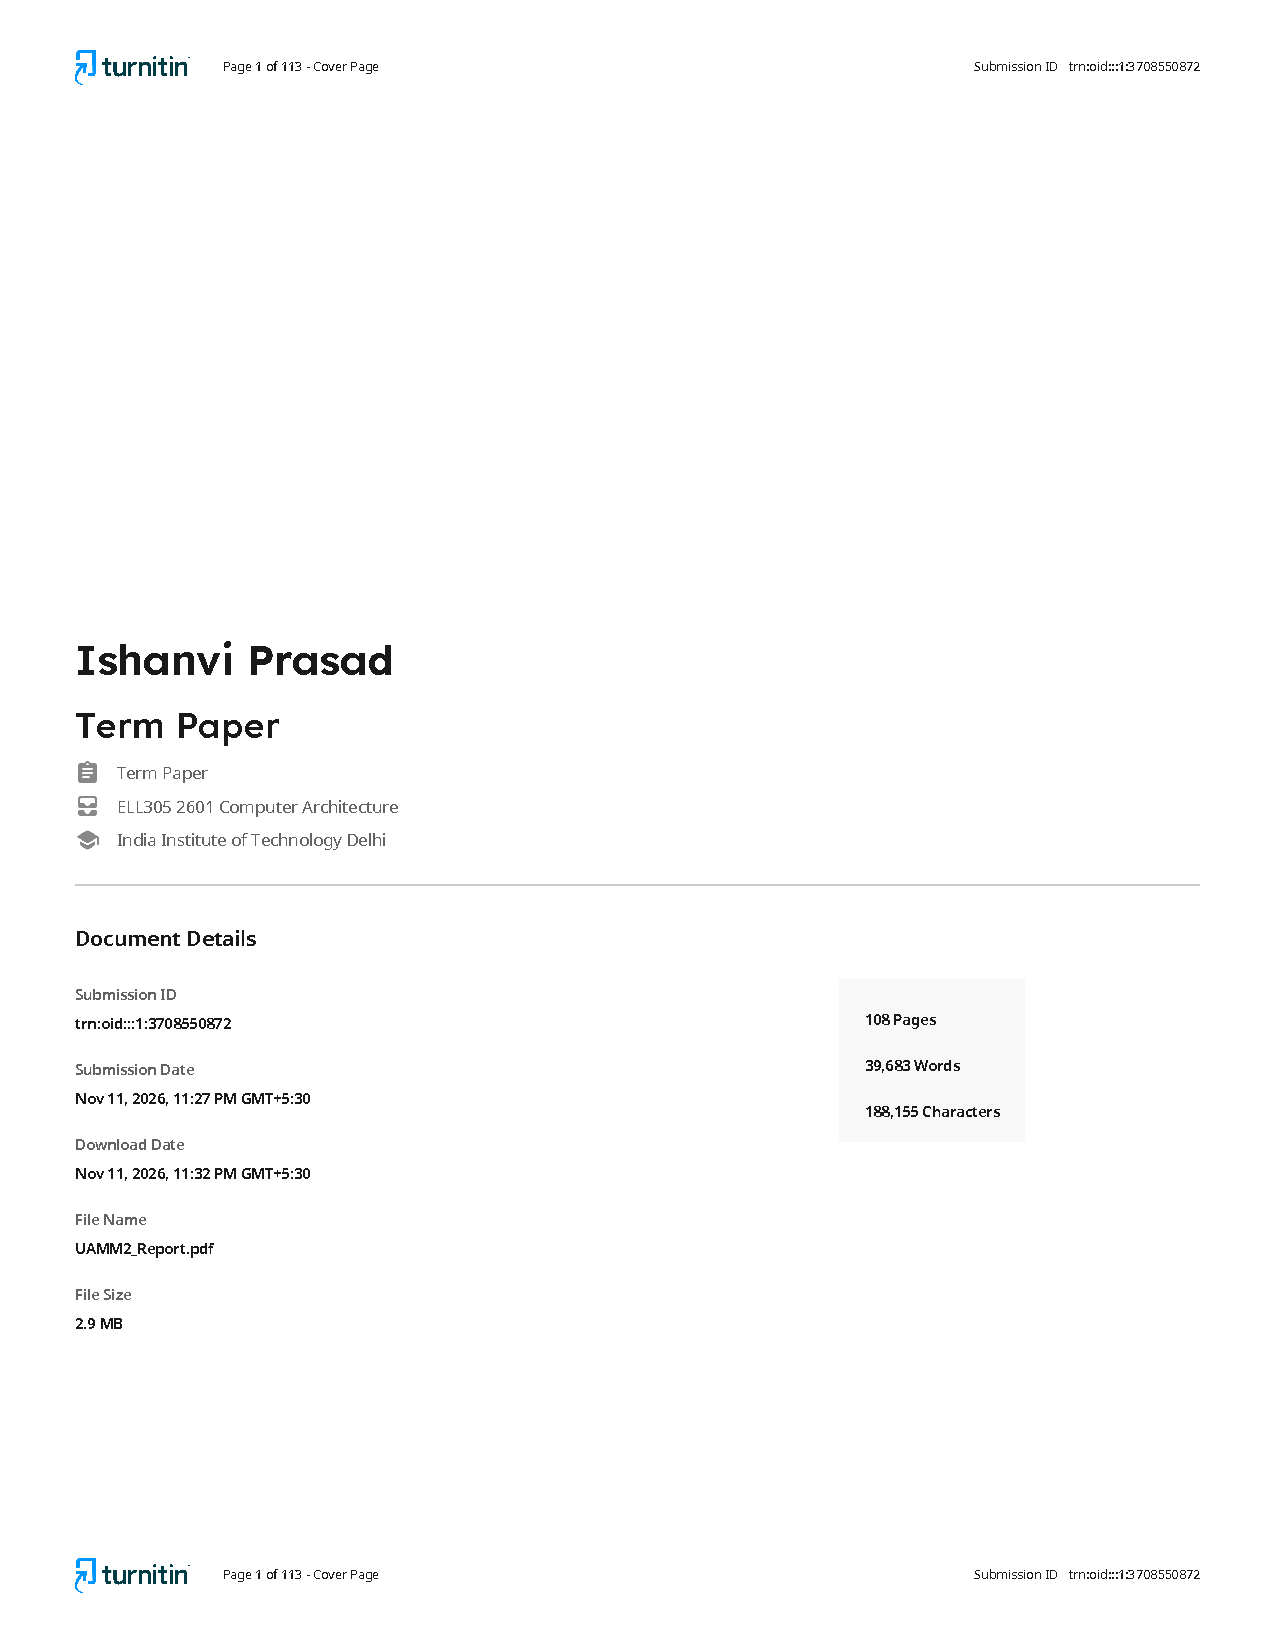
\includepdf[pages={1-5},scale=0.92,pagecommand={\thispagestyle{plain}}]{figs/turnitin_pages_1-5.pdf}
\chapter{Readability Indices}\label{app:readability}
We measured the running prose of the main chapters (Chapters 1 to 9: paragraphs, bullet points and boxes; tables, captions, equations, code and appendices excluded). The indices are computed by our own script with the usual published formulas. Syllables are counted with a rule-based heuristic, so the values are approximate. The method follows the description at analyzemywriting.com/readability\_\allowbreak{}indices.html.

{\fontsize{9}{10.5}\selectfont\setlength{\tabcolsep}{3pt}
\begin{longtable}{>{\raggedright\arraybackslash}p{3.64in}>{\raggedright\arraybackslash}p{2.42in}}
\caption{Counts used for the readability indices.}\\
\toprule
\textbf{Quantity} & \textbf{Value} \\\midrule\endfirsthead
\toprule \textbf{Quantity} & \textbf{Value} \\\midrule\endhead
\bottomrule\endfoot
Words & 19,117 \\
Sentences & 1,098 \\
Words per sentence & 17.4 \\
Syllables per word & 1.50 \\
Words of three or more syllables & 11.7 \% \\
\bottomrule
\end{longtable}}
{\fontsize{9}{10.5}\selectfont\setlength{\tabcolsep}{3pt}
\begin{longtable}{>{\raggedright\arraybackslash}p{1.99in}>{\raggedright\arraybackslash}p{0.72in}>{\raggedright\arraybackslash}p{3.25in}}
\caption{Readability indices of the main text.}\\
\toprule
\textbf{Index} & \textbf{Value} & \textbf{What it means} \\\midrule\endfirsthead
\toprule \textbf{Index} & \textbf{Value} & \textbf{What it means} \\\midrule\endhead
\bottomrule\endfoot
Flesch Reading Ease & 62.1 & 0 to 100; higher is easier. 30 to 50 is difficult, college level. \\
Flesch-Kincaid Grade Level & 8.9 & US school grade needed to follow the text. \\
Gunning Fog & 11.6 & Years of schooling needed; 12 is the level of a senior high-school student. \\
SMOG & 11.3 & Grade level from the count of long words per sentence. \\
Coleman-Liau & 10.0 & Grade level from letters per word and sentences per 100 words. \\
Automated Readability Index & 9.3 & Grade level from characters per word and words per sentence. \\
\bottomrule
\end{longtable}}
A Flesch Reading Ease of about 62 and grade levels between 9 and 12 put the text at the level of plain, careful technical English. The long words are mostly terms (quantisation\index{quantisation}, hysteresis\index{hysteresis}, heterogeneous) that we could not replace.

\chapter{Raw Experiment Tables}\label{app:rawtables}
Mean ± standard deviation over seeds. Columns: resident / FP16\index{FP16}, dropped tokens, mean relative L2 error, 95th-percentile error, attention-mass recall\index{recall}, modelled fetch ms per token, flash\index{flash} reads, migrations, re-encodes, overflow bytes.

{\fontsize{8}{9.5}\selectfont\setlength{\tabcolsep}{3pt}
\begin{longtable}{>{\raggedright\arraybackslash}p{1.22in}>{\raggedright\arraybackslash}p{0.95in}>{\raggedright\arraybackslash}p{0.77in}>{\raggedright\arraybackslash}p{0.95in}>{\raggedright\arraybackslash}p{0.90in}>{\raggedright\arraybackslash}p{0.90in}}
\caption{E1 ablation (5 seeds, 1,536 tokens) (columns 1 to 5)}\\
\toprule
\textbf{setting} & \textbf{res/FP16} & \textbf{drop} & \textbf{err} & \textbf{err p95} & \textbf{recall} \\\midrule\endfirsthead
\toprule \textbf{setting} & \textbf{res/FP16} & \textbf{drop} & \textbf{err} & \textbf{err p95} & \textbf{recall} \\\midrule\endhead
\bottomrule\endfoot
v1\_\allowbreak{}threshold\_\allowbreak{}fp16 & 0.3667 ± 0.01019 & 972.8 ± 15.68 & 0.4789 ± 0.03459 & 1.288 ± 0.1304 & 0.7581 ± 0.01638 \\
v1\_\allowbreak{}capacity\_\allowbreak{}aware\_\allowbreak{}fp16 & 0.4062 ± 0 & 912 ± 0 & 0.4056 ± 0.03049 & 1.142 ± 0.08034 & 0.7917 ± 0.01163 \\
static\_\allowbreak{}kivi4\_\allowbreak{}no\_\allowbreak{}planner & 0.3643 ± 0 & 0 ± 0 & 0.1519 ± 0.01504 & 0.3679 ± 0.06149 & 0.9389 ± 0.0117 \\
static\_\allowbreak{}kivi2\_\allowbreak{}no\_\allowbreak{}planner & 0.2432 ± 0 & 0 ± 0 & 0.5716 ± 0.01873 & 1.022 ± 0.06567 & 0.9389 ± 0.0117 \\
v2\_\allowbreak{}planner\_\allowbreak{}fp16 & 1 ± 0 & 0 ± 0 & 0.09209 ± 0.01912 & 0.3312 ± 0.07139 & 0.9389 ± 0.0117 \\
v2\_\allowbreak{}planner\_\allowbreak{}int8\_\allowbreak{}kivi4 & 0.3711 ± 0.002651 & 0 ± 0 & 0.1224 ± 0.01366 & 0.3614 ± 0.06096 & 0.9389 ± 0.0117 \\
v2\_\allowbreak{}planner\_\allowbreak{}all\_\allowbreak{}codecs & 0.3101 ± 0.001326 & 0 ± 0 & 0.1662 ± 0.02025 & 0.5709 ± 0.1013 & 0.9389 ± 0.0117 \\
v2\_\allowbreak{}all\_\allowbreak{}codecs\_\allowbreak{}with\_\allowbreak{}drop & 0.3101 ± 0.001326 & 0 ± 0 & 0.1662 ± 0.02025 & 0.5709 ± 0.1013 & 0.9389 ± 0.0117 \\
\bottomrule
\end{longtable}}
{\fontsize{8}{9.5}\selectfont\setlength{\tabcolsep}{3pt}
\begin{longtable}{>{\raggedright\arraybackslash}p{1.25in}>{\raggedright\arraybackslash}p{1.02in}>{\raggedright\arraybackslash}p{0.97in}>{\raggedright\arraybackslash}p{0.79in}>{\raggedright\arraybackslash}p{0.79in}>{\raggedright\arraybackslash}p{0.88in}}
\caption{E1 ablation (5 seeds, 1,536 tokens) (columns 6 to 10)}\\
\toprule
\textbf{setting} & \textbf{fetch ms} & \textbf{flash} & \textbf{migr} & \textbf{reenc} & \textbf{overflow B} \\\midrule\endfirsthead
\toprule \textbf{setting} & \textbf{fetch ms} & \textbf{flash} & \textbf{migr} & \textbf{reenc} & \textbf{overflow B} \\\midrule\endhead
\bottomrule\endfoot
v1\_\allowbreak{}threshold\_\allowbreak{}fp16 & 0.9229 ± 0.02585 & 1.261e+04 ± 374 & 744.8 ± 35.78 & 0 ± 0 & 0 ± 0 \\
v1\_\allowbreak{}capacity\_\allowbreak{}aware\_\allowbreak{}fp16 & 0.6181 ± 0.008936 & 8205 ± 129.2 & 883 ± 60.1 & 0 ± 0 & 0 ± 0 \\
static\_\allowbreak{}kivi4\_\allowbreak{}no\_\allowbreak{}planner & 0.06814 ± 0.002529 & 270 ± 37.5 & 694.2 ± 38.49 & 93 ± 0 & 0 ± 0 \\
static\_\allowbreak{}kivi2\_\allowbreak{}no\_\allowbreak{}planner & 0.0493 ± 4e-06 & 0 ± 0 & 309.8 ± 24.6 & 93 ± 0 & 0 ± 0 \\
v2\_\allowbreak{}planner\_\allowbreak{}fp16 & 1.041 ± 0.005997 & 1.436e+04 ± 86.17 & 628.6 ± 18.78 & 0 ± 0 & 2.58e+05 ± 1832 \\
v2\_\allowbreak{}planner\_\allowbreak{}int8\_\allowbreak{}kivi4 & 0.1156 ± 0.002161 & 969.6 ± 32.11 & 698.6 ± 25.26 & 178.8 ± 1.6 & 0 ± 0 \\
v2\_\allowbreak{}planner\_\allowbreak{}all\_\allowbreak{}codecs & 0.1117 ± 0.002028 & 915 ± 30.09 & 644.4 ± 21.27 & 225.6 ± 1.625 & 0 ± 0 \\
v2\_\allowbreak{}all\_\allowbreak{}codecs\_\allowbreak{}with\_\allowbreak{}drop & 0.1117 ± 0.002028 & 915 ± 30.09 & 644.4 ± 21.27 & 225.6 ± 1.625 & 0 ± 0 \\
\bottomrule
\end{longtable}}
{\fontsize{8}{9.5}\selectfont\setlength{\tabcolsep}{3pt}
\begin{longtable}{>{\raggedright\arraybackslash}p{0.61in}>{\raggedright\arraybackslash}p{1.23in}>{\raggedright\arraybackslash}p{0.50in}>{\raggedright\arraybackslash}p{1.11in}>{\raggedright\arraybackslash}p{1.11in}>{\raggedright\arraybackslash}p{1.11in}}
\caption{E4 quality weight lambda (columns 1 to 5)}\\
\toprule
\textbf{setting} & \textbf{res/FP16} & \textbf{drop} & \textbf{err} & \textbf{err p95} & \textbf{recall} \\\midrule\endfirsthead
\toprule \textbf{setting} & \textbf{res/FP16} & \textbf{drop} & \textbf{err} & \textbf{err p95} & \textbf{recall} \\\midrule\endhead
\bottomrule\endfoot
0.0 & 0.2432 ± 0 & 0 ± 0 & 0.5772 ± 0.01988 & 1.043 ± 0.07619 & 0.9454 ± 0.01103 \\
0.25 & 0.264 ± 0.001838 & 0 ± 0 & 0.2893 ± 0.01638 & 0.7877 ± 0.06544 & 0.9454 ± 0.01103 \\
0.5 & 0.2835 ± 0.002123 & 0 ± 0 & 0.2003 ± 0.02808 & 0.6013 ± 0.1195 & 0.9454 ± 0.01103 \\
1.0 & 0.2948 ± 0.0006128 & 0 ± 0 & 0.1815 ± 0.03109 & 0.5715 ± 0.1199 & 0.9454 ± 0.01103 \\
2.0 & 0.3096 ± 0.001061 & 0 ± 0 & 0.1592 ± 0.02339 & 0.5361 ± 0.1069 & 0.9454 ± 0.01103 \\
4.0 & 0.3152 ± 0.002671 & 0 ± 0 & 0.1523 ± 0.02454 & 0.5262 ± 0.1153 & 0.9454 ± 0.01103 \\
8.0 & 0.3252 ± 0.003184 & 0 ± 0 & 0.1382 ± 0.01213 & 0.4728 ± 0.07563 & 0.9454 ± 0.01103 \\
16.0 & 0.3434 ± 0.003677 & 0 ± 0 & 0.1341 ± 0.01333 & 0.4557 ± 0.06814 & 0.9454 ± 0.01103 \\
32.0 & 0.3656 ± 0.006457 & 0 ± 0 & 0.127 ± 0.008716 & 0.4326 ± 0.05711 & 0.9454 ± 0.01103 \\
\bottomrule
\end{longtable}}
{\fontsize{8}{9.5}\selectfont\setlength{\tabcolsep}{3pt}
\begin{longtable}{>{\raggedright\arraybackslash}p{0.64in}>{\raggedright\arraybackslash}p{1.28in}>{\raggedright\arraybackslash}p{0.99in}>{\raggedright\arraybackslash}p{0.99in}>{\raggedright\arraybackslash}p{0.99in}>{\raggedright\arraybackslash}p{0.81in}}
\caption{E4 quality weight lambda (columns 6 to 10)}\\
\toprule
\textbf{setting} & \textbf{fetch ms} & \textbf{flash} & \textbf{migr} & \textbf{reenc} & \textbf{overflow B} \\\midrule\endfirsthead
\toprule \textbf{setting} & \textbf{fetch ms} & \textbf{flash} & \textbf{migr} & \textbf{reenc} & \textbf{overflow B} \\\midrule\endhead
\bottomrule\endfoot
0.0 & 0.09789 ± 0.002523 & 723.7 ± 37.56 & 572.7 ± 6.944 & 93 ± 0 & 0 ± 0 \\
0.25 & 0.101 ± 0.001069 & 763 ± 16.08 & 610.3 ± 18.35 & 175.7 ± 1.7 & 0 ± 0 \\
0.5 & 0.1062 ± 0.002955 & 836.3 ± 43.76 & 631 ± 10.98 & 188.3 ± 2.494 & 0 ± 0 \\
1.0 & 0.1079 ± 0.003259 & 859.7 ± 48.4 & 639.3 ± 16.94 & 213.7 ± 3.3 & 0 ± 0 \\
2.0 & 0.1112 ± 0.00247 & 907.7 ± 36.75 & 629.7 ± 14.52 & 226.3 ± 1.7 & 0 ± 0 \\
4.0 & 0.1973 ± 0.03053 & 2189 ± 455.1 & 567 ± 5.715 & 226.3 ± 2.867 & 0 ± 0 \\
8.0 & 0.2453 ± 0.003006 & 2912 ± 44.85 & 567.3 ± 24.28 & 222.7 ± 1.247 & 0 ± 0 \\
16.0 & 0.237 ± 0.004147 & 2792 ± 60.42 & 613.7 ± 20.29 & 214.7 ± 1.886 & 0 ± 0 \\
32.0 & 0.2535 ± 0.006791 & 3036 ± 101.6 & 726 ± 52.71 & 205 ± 3.559 & 0 ± 0 \\
\bottomrule
\end{longtable}}
{\fontsize{8}{9.5}\selectfont\setlength{\tabcolsep}{3pt}
\begin{longtable}{>{\raggedright\arraybackslash}p{0.61in}>{\raggedright\arraybackslash}p{1.17in}>{\raggedright\arraybackslash}p{0.50in}>{\raggedright\arraybackslash}p{1.17in}>{\raggedright\arraybackslash}p{1.11in}>{\raggedright\arraybackslash}p{1.11in}}
\caption{E5 capacity factor, combined system (columns 1 to 5)}\\
\toprule
\textbf{setting} & \textbf{res/FP16} & \textbf{drop} & \textbf{err} & \textbf{err p95} & \textbf{recall} \\\midrule\endfirsthead
\toprule \textbf{setting} & \textbf{res/FP16} & \textbf{drop} & \textbf{err} & \textbf{err p95} & \textbf{recall} \\\midrule\endhead
\bottomrule\endfoot
0.5 & 0.2878 ± 0.008107 & 0 ± 0 & 0.2204 ± 0.0104 & 0.6296 ± 0.03874 & 0.9454 ± 0.01103 \\
0.75 & 0.2935 ± 0.002671 & 0 ± 0 & 0.1801 ± 0.02752 & 0.5765 ± 0.1167 & 0.9454 ± 0.01103 \\
1.0 & 0.3096 ± 0.001061 & 0 ± 0 & 0.1592 ± 0.02339 & 0.5361 ± 0.1069 & 0.9454 ± 0.01103 \\
1.5 & 0.3226 ± 0.004246 & 0 ± 0 & 0.1306 ± 0.009824 & 0.4271 ± 0.06095 & 0.9454 ± 0.01103 \\
2.0 & 0.33 ± 0.001621 & 0 ± 0 & 0.115 ± 0.01631 & 0.3613 ± 0.06399 & 0.9454 ± 0.01103 \\
3.0 & 0.3239 ± 0.002808 & 0 ± 0 & 0.1518 ± 0.02296 & 0.5418 ± 0.09728 & 0.9454 ± 0.01103 \\
\bottomrule
\end{longtable}}
{\fontsize{8}{9.5}\selectfont\setlength{\tabcolsep}{3pt}
\begin{longtable}{>{\raggedright\arraybackslash}p{0.60in}>{\raggedright\arraybackslash}p{1.24in}>{\raggedright\arraybackslash}p{0.92in}>{\raggedright\arraybackslash}p{0.92in}>{\raggedright\arraybackslash}p{0.92in}>{\raggedright\arraybackslash}p{1.08in}}
\caption{E5 capacity factor, combined system (columns 6 to 10)}\\
\toprule
\textbf{setting} & \textbf{fetch ms} & \textbf{flash} & \textbf{migr} & \textbf{reenc} & \textbf{overflow B} \\\midrule\endfirsthead
\toprule \textbf{setting} & \textbf{fetch ms} & \textbf{flash} & \textbf{migr} & \textbf{reenc} & \textbf{overflow B} \\\midrule\endhead
\bottomrule\endfoot
0.5 & 0.3011 ± 0.01844 & 3729 ± 272.7 & 863.7 ± 35.46 & 200.7 ± 5.437 & 3.311e+04 ± 3205 \\
0.75 & 0.1415 ± 0.005091 & 1360 ± 76.25 & 804.7 ± 40.14 & 229.7 ± 1.7 & 0 ± 0 \\
1.0 & 0.1112 ± 0.00247 & 907.7 ± 36.75 & 629.7 ± 14.52 & 226.3 ± 1.7 & 0 ± 0 \\
1.5 & 0.09922 ± 0.002136 & 728 ± 30.69 & 594.3 ± 9.672 & 221.3 ± 3.3 & 0 ± 0 \\
2.0 & 0.08823 ± 0.002131 & 566.3 ± 29.51 & 548.3 ± 15.54 & 217 ± 0.8165 & 0 ± 0 \\
3.0 & 0.04853 ± 0.0003229 & 3.333 ± 4.028 & 162 ± 6.532 & 225.7 ± 1.247 & 0 ± 0 \\
\bottomrule
\end{longtable}}
\chapter{Core Source Listings}\label{app:listings}
The complete project is supplied as a separate archive; the listings below are the parts the report describes most closely. The remaining files are in the repository.

\par\smallskip\noindent\textbf{hw/rtl/uamm\_\allowbreak{}sweep\_\allowbreak{}scorer.v}\par\nopagebreak
\begin{lstlisting}
// UAMM-2 sweep scorer: hardware "heat classifier" for the block table.
//
// Replaces the single-shot uamm_controller of UAMM-1:
//   * no divider: weights are integers summing to 256 (154/64/38 ~= 60%/25%/15%), score = sum >> 8
//   * block metadata lives in a small SRAM; one sweep streams every block through a 2-stage pipeline
//     (1 block/cycle) so thousands of blocks are scored per planner interval
//   * `protected` (sink / recent window) is honoured in hardware, matching the Python planner
//
// Metadata word (25 bits): {protected, frequency[7:0], recency[7:0], importance[7:0]}
// Output tier code: 2'b00 hot (T0/T1), 2'b01 warm (T2), 2'b10 cold (T3).
// Synthesizable Verilog-2001.
module uamm_sweep_scorer #(
    parameter NBLK = 64,
    parameter AW   = 6            // AW = log2(NBLK)
) (
    input  wire          clk,
    input  wire          rst_n,
    // metadata write port
    input  wire          we,
    input  wire [AW-1:0] waddr,
    input  wire [24:0]   wdata,
    // sweep control
    input  wire          start,       // ignored while busy
    input  wire [7:0]    pressure,    // memory pressure, latched at start
    output reg           busy,
    output reg           done,        // pulses with the last out_valid of a sweep
    // result stream
    output reg           out_valid,
    output reg  [AW-1:0] out_idx,
    output reg  [7:0]    out_score,
    output reg  [1:0]    out_tier,
    output reg           out_evict
);
    localparam [7:0] W_IMP   = 8'd154;
    localparam [7:0] W_REC   = 8'd64;
    localparam [7:0] W_FRQ   = 8'd38;
    localparam [7:0] TH_HOT  = 8'd174;
    localparam [7:0] TH_WARM = 8'd89;
    localparam [7:0] EVICT_P = 8'd243;

    reg [24:0] mem [0:NBLK-1];
    always @(posedge clk) if (we) mem[waddr] <= wdata;

    reg [AW:0]    rd_cnt;
    reg [7:0]     pres;
    reg           s0_v;
    reg [AW-1:0]  s0_idx;
    reg [24:0]    s0_data;

    // synchronous SRAM read, address = issue counter
    always @(posedge clk) s0_data <= mem[rd_cnt[AW-1:0]];

    wire [7:0]  imp   = s0_data[7:0];
    wire [7:0]  rec   = s0_data[15:8];
    wire [7:0]  frq   = s0_data[23:16];
    wire        prot  = s0_data[24];
    /* verilator lint_off UNUSEDSIGNAL */
    wire [15:0] wsum  = (imp * W_IMP) + (rec * W_REC) + (frq * W_FRQ);  // <= 255*256
    /* verilator lint_on UNUSEDSIGNAL */
    wire [7:0]  score = wsum[15:8];   // wsum[7:0] intentionally dropped (>> 8)
    wire [1:0]  tier  = prot ? 2'b00 :
                        (score >= TH_HOT)  ? 2'b00 :
                        (score >= TH_WARM) ? 2'b01 : 2'b10;
    wire        evict = (!prot) && (pres >= EVICT_P) && (score < TH_WARM);
    localparam [31:0] LAST_IDX = NBLK - 1;
    wire        last  = s0_v && ({{(32-AW){1'b0}}, s0_idx} == LAST_IDX);

    always @(posedge clk or negedge rst_n) begin
        if (!rst_n) begin
            busy <= 1'b0;  done <= 1'b0;  rd_cnt <= {(AW+1){1'b0}};  pres <= 8'd0;
            s0_v <= 1'b0;  s0_idx <= {AW{1'b0}};
            out_valid <= 1'b0;  out_idx <= {AW{1'b0}};  out_score <= 8'd0;
            out_tier <= 2'b10;  out_evict <= 1'b0;
        end else begin
            // ---- stage 1: score the block read last cycle
            out_valid <= s0_v;
            done      <= last;
            if (s0_v) begin
                out_idx   <= s0_idx;
                out_score <= score;
                out_tier  <= tier;
                out_evict <= evict;
            end
            // ---- stage 0: issue reads
            if (start && !busy) begin
                busy <= 1'b1;  rd_cnt <= {(AW+1){1'b0}};  pres <= pressure;  s0_v <= 1'b0;
            end else if (busy && (rd_cnt < NBLK)) begin
                s0_v   <= 1'b1;
                s0_idx <= rd_cnt[AW-1:0];
                rd_cnt <= rd_cnt + 1'b1;
            end else begin
                s0_v <= 1'b0;
            end
            if (last) busy <= 1'b0;
        end
    end
endmodule
\end{lstlisting}
\chapter{UAMM-1 Source Code (Original Prototype)}\label{app:uamm1src}
This appendix reproduces, unchanged, the prototype that Chapter~4 analyses: the Verilog controller and its testbench (the Python modules are in the repository). The concatenated listings are also stored in the archive under \texttt{uamm1\_\allowbreak{}\allowbreak{}original/\allowbreak{}}. They are the authors' own earlier code and are included so that the comparison of UAMM-1\index{UAMM-1} and UAMM-2\index{UAMM-2} can be checked against the actual implementation.

The Python modules of UAMM-1\index{UAMM-1} are not reproduced here because of their length; they are in \texttt{uamm1\_\allowbreak{}\allowbreak{}original/\allowbreak{}uamm1\_\allowbreak{}\allowbreak{}python\_\allowbreak{}\allowbreak{}listing.\allowbreak{}txt} in the repository.

\par\smallskip\noindent\textbf{D.1  UAMM-1 Verilog controller and testbench}\par\nopagebreak
\begin{lstlisting}
`timescale 1ns/1ps
module tb_uamm_controller;
    reg clk = 0;
    always #5 clk = ~clk;
    reg rst_n = 0, valid = 0;
    reg [7:0] importance, recency, frequency, memory_pressure;
    wire out_valid, evict;
    wire [7:0] score;
    wire [1:0] tier;

    uamm_controller dut(.clk(clk), .rst_n(rst_n), .valid(valid),
        .importance(importance), .recency(recency), .frequency(frequency),
        .memory_pressure(memory_pressure), .out_valid(out_valid),
        .score(score), .tier(tier), .evict(evict));

    task apply;
        input [7:0] h, r, f, p;
        input [1:0] expected_tier;
        input expected_evict;
        begin
            @(negedge clk);
            valid=1; importance=h; recency=r; frequency=f; memory_pressure=p;
            @(posedge clk); #1;
            if (!out_valid || tier !== expected_tier || evict !== expected_evict) begin
                $display("FAIL h=%0d r=%0d f=%0d p=%0d score=%0d tier=%b evict=%b",
                         h,r,f,p,score,tier,evict);
                $fatal(1);
            end
        end
    endtask

    initial begin
        importance=0; recency=0; frequency=0; memory_pressure=0;
        repeat(2) @(posedge clk);
        rst_n=1;
        apply(8'd255,8'd255,8'd255,8'd0,2'b00,1'b0);
        apply(8'd150,8'd100,8'd80,8'd0,2'b01,1'b0);
        apply(8'd10,8'd10,8'd10,8'd255,2'b10,1'b1);
        $display("PASS: controller decisions");
        $finish;
    end
endmodule

// UAMM policy decision engine - synthesizable Verilog-2001.
// Inputs are normalized unsigned 8-bit values (0..255).
module uamm_controller (
    input wire        clk,
    input wire        rst_n,
    input wire        valid,
    input wire [7:0] importance,
    input wire [7:0] recency,
    input wire [7:0] frequency,
    input wire [7:0] memory_pressure,
    output reg        out_valid,
    output reg [7:0] score,
    output reg [1:0] tier,        // 00 GPU, 01 CPU, 10 NVMe
    output reg        evict
);
    // Weighted score: 60% importance + 25% recency + 15% frequency.
    // Sum of weights is 100; divide by 100 to retain 8-bit scale.
    wire [15:0] weighted_sum =
        (importance * 8'd60) +
        (recency    * 8'd25) +
        (frequency * 8'd15);
    wire [7:0] computed_score = weighted_sum / 16'd100;

    always @(posedge clk or negedge rst_n) begin
        if (!rst_n) begin
            out_valid <= 1'b0;
            score       <= 8'd0;
            tier        <= 2'b10;
            evict       <= 1'b0;
        end else begin
            out_valid <= valid;
            if (valid) begin
                 score <= computed_score;
                 if (computed_score >= 8'd174)
                      tier <= 2'b00; // GPU
                 else if (computed_score >= 8'd89)
                      tier <= 2'b01; // CPU
                 else
                      tier <= 2'b10; // NVMe

                  evict <= (memory_pressure >= 8'd243) &&
                           (computed_score < 8'd89);
              end else begin
                  evict <= 1'b0;
              end
        end
    end
endmodule
\end{lstlisting}
\clearpage\listoftables\clearpage\listoffigures\clearpage\glsaddall\printglossary[title={Glossary}]\clearpage\printindex
\end{document}
